%%%%%%%%%%%%%%%%%%% vorlage.tex %%%%%%%%%%%%%%%%%%%%%%%%%%%%%
%
% LaTeX-Vorlage zur Erstellung von Projekt-Dokumentationen
% im Fachbereich Informatik der Hochschule Trier
%
% Basis: Vorlage svmono des Springer Verlags
%
%%%%%%%%%%%%%%%%%%%%%%%%%%%%%%%%%%%%%%%%%%%%%%%%%%%%%%%%%%%%%

\documentclass[envcountsame,envcountchap, deutsch]{i-studis}

\usepackage{footnote}
\usepackage[LGR,T1]{fontenc}
\usepackage{float}
\usepackage{python}
\usepackage{xparse}
\usepackage{enumitem}
\usepackage[outputdir=../../auxil]{minted}
\usepackage{comment}
\usepackage[normalem]{ulem}
\usepackage[inkscapeformat=png]{svg}
\usepackage[titles]{tocloft}
\usepackage{titlesec}
\usepackage[pdftex,plainpages=false]{hyperref}
\usepackage{xurl}
\usepackage[toc]{glossaries}
\usepackage[titletoc,title,page, header]{appendix} % Anhang
\usepackage[backend=biber, style=alphabetic, isbn=true, doi=true]{biblatex}
\usepackage{makeidx}         	% Index
\usepackage{multicol}% Zweispaltiger Index
\usepackage[threshold=0]{csquotes}
\usepackage{soul}
\usepackage{caption}
\usepackage{makecell}

\setcounter{tocdepth}{4}
\setcounter{secnumdepth}{6}

\captionsetup{font=small}
\captionsetup{labelfont=bf}

\newcommand{\textgreek}[1]{\begingroup\fontencoding{LGR}\selectfont#1\endgroup}

\BeforeBeginEnvironment{tcolorbox}{\savenotes}
\AfterEndEnvironment{tcolorbox}{\spewnotes}

%\usepackage[bottom]{footmisc}	% Erzeugung von Fu�noten

%%-----------------------------------------------------
%\newif\ifpdf
%\ifx\pdfoutput\undefined
%\pdffalse
%\else
%\pdfoutput=1
%\pdftrue
%\fi
%%--------------------------------------------------------
%\ifpdf
\usepackage[pdftex]{graphicx}
\usepackage{epstopdf}

\usepackage{tcolorbox}
\usepackage[table]{colortbl}% http://ctan.org/pkg/xcolor
%\else
%\usepackage{graphicx}
%\usepackage[plainpages=false]{hyperref}
%\fi

%%-----------------------------------------------------
\usepackage{color}				% Farbverwaltung
%\usepackage{ngerman} 			% Neue deutsche Rechtsschreibung
\usepackage[english, ngerman]{babel}

\renewcommand\appendixpagename{Anhänge}
\renewcommand\appendixtocname{Anhänge}
%%-----------------------------------------------------
% Unterscheidung für Umlaute Windows-Mac
%%-----------------------------------------------------

%\usepackage[latin1]{inputenc} 	% Ermöglicht Umlaute-Darstellung
\usepackage[utf8]{inputenc}  	% Ermöglicht Umlaute-Darstellung unter Linux (je nach verwendetem Format)

%-----------------------------------------------------
\usepackage{listings} 			% Code-Darstellung
\lstset
{
	basicstyle=\scriptsize, 	% print whole listing small
	keywordstyle=\color{blue}\bfseries,
% underlined bold black keywords
	identifierstyle=, 			% nothing happens
	commentstyle=\color{red}, 	% white comments
	stringstyle=\ttfamily, 		% typewriter type for strings
	showstringspaces=false, 	% no special string spaces
	framexleftmargin=7mm,
	tabsize=3,
	showtabs=false,
	captionpos=b,
	frame=single,
	rulesepcolor=\color{blue},
	numbers=left,
	linewidth=146mm,
	xleftmargin=8mm
}

\NewDocumentCommand{\code}{v}{%
	\texttt{\textcolor{blue}{#1}}%
}
\NewDocumentCommand{\staticcode}{v}{%
	\ul{{\texttt{\textcolor{blue}{#1}}}}%
}



\usepackage{textcomp} 			% Celsius-Darstellung
\usepackage{amssymb,amsfonts,amstext,amsmath}	% Mathematische Symbole
\usepackage[german, ruled, vlined]{algorithm2e}
\usepackage[a4paper]{geometry} % Andere Formatierung
\usepackage{bibgerm}
\usepackage{array}
\usepackage{mathtools}
\usepackage{mdwtab}
\usepackage{datagidx}
\usepackage{lstmisc}
\hyphenation{Ele-men-tar-ob-jek-te  ab-ge-tas-tet Aus-wer-tung House-holder-Matrix Le-ast-Squa-res-Al-go-ri-th-men} 		% Weitere Silbentrennung bei Bedarf angeben
\setlength{\textheight}{1.1\textheight}
\pagestyle{myheadings} 			% Erzeugt selbstdefinierte Kopfzeile
\makeindex 						% Index-Erstellung

% uncomment to hide tables, equations and figures
%\excludecomment{confidential}
%\excludecomment{figure}
%\excludecomment{equation}
%\excludecomment{table}
%\let\endfigure\relax
%\let\endtable\relax
%\let\endequation\relax


\DeclareFieldFormat{doi}{\textsc{doi}: \texttt{#1}}
\DeclareFieldFormat{isbn}{\textsc{isbn}: \texttt{#1}}

\DeclareFieldFormat{postnote}{#1}
\DeclareFieldFormat{multipostnote}{#1}

\addbibresource{literatur.bib}


\newglossarystyle{mystyle}{%
	\setglossarystyle{treegroup}%

	\renewcommand*{\glossentry}[2]{%
		\glsentryitem{##1}\textbf{\glstarget{##1}{\glossentryname{##1}}}%
		\par
		\glossentrydesc{##1}
		\par
		\vspace{1cm}
	}%
}

\setglossarystyle{mystyle}


\makenoidxglossaries
\loadglsentries{chapters/Glossar/index.tex}

%--------------------------------------------------------------------------
\begin{document}

%------------------------- Titelblatt -------------------------------------
	\title{\begin{center}
			   Repetitorium SE

			   \textbf{}\\
			   \\

			   \\
			   \small{Modul se, SS 24} \\ \small{Trier University of Applied Sciences}\\ \small{Informatik Fernstudium (M.C.Sc.)}
	\end{center}}
	\project{}
%--------------------------------------------------------------------------
	\supervisor{Titel Vorname Name} 		% Betreuer der Arbeit
	\author{\begin{center}

	\end{center}}							% Autor der Arbeit
	\address{\begin{center}
				 \small{09.07.2024\\  Thorsten Suckow-Homberg, \url{https://thorsten.suckow-homberg.de}}
	\end{center}} 							% Im Zusammenhang mit dem Datum wird hinter dem Ort ein Komma angegeben
	\submitdate{} 				% Abgabedatum
%\begingroup
%  \renewcommand{\thepage}{title}
%  \mytitlepage
%  \newpage
%\endgroup



	\begingroup
	\renewcommand{\thepage}{Titel}
	\mytitlepage
	\newpage
	\endgroup
%--------------------------------------------------------------------------
	\frontmatter
%--------------------------------------------------------------------------
	\section*{Hinweise}
Modulbegleitende (Mit-)Schrift, die sich überwiegend auf \cite{Wed09}, \cite{Wed09b} sowie \cite{Buh09} bezieht.
	\tableofcontents 						% Inhaltsverzeichnis
%--------------------------------------------------------------------------
	\mainmatter                        		% Hauptteil (ab hier arab. Seitenzahlen)
%--------------------------------------------------------------------------
% Die Kapitel werden in separaten .tex-Dateien abgelegt und hier eingebunden.
	\part{Teil 1 - Grundlagen der Softwaretechnik und Requirements Engineering}

\vspace{2cm}
\blockquote[{\url{https://fg-swt.gi.de}\footnote{abgerufen 04.04.2024}}]{``Unter \textbf{Softwaretechnik} (engl. \textit{Software Engineering}) versteht man allgemein die (Ingenieur-) Wissenschaft, die die kosteneffiziente Entwicklung von qualitativ hochwertiger Software behandelt.``}
\vspace{2cm}
\blockquote[{\cite[247]{BMEY07}}]{
    ``The amateur software engineer is always in search
    of magic, some sensational method or tool whose
    application promises to render software development trivial. It is the mark of the professional software engineer to know that no such panacea exists.
    Amateurs often want to follow cookbook steps; professionals know that right approaches to development usually lead to inept design products, born of a
    progression of lies and behind which developers can
    shield themselves from accepting responsibility for
    earlier misguided decisions. The amateur software
    engineer either ignores documentation all together,
    or follows a process that is documentation-driven,
    worrying more about how these paper products look
    to the customer than about the substance they contain. The professional acknowledges the importance
    of creating certain documents, but never does so at
    the expense of making sensible architectural innovations.``
}

\newpage
\section*{Lernziele Teil 1}

\begin{itemize}
    \item die Aufgaben und Ziele  des Software Engineerings kennen
    \item mit den Phasen des Entwicklungszyklus und ihren Inhalten vertraut sein
    \item einen Überblick über existierende Vorgehensmodelle besitzen und ihre Anwendbarkeit auf Problemstellungen beurteilen können
    \item in der Lage sein, Anforderungen geeignet aufzunehmen und schriftlich zu erfassen
\end{itemize}

\newpage
	

\section{Inhalt SE3}

\section*{1. Übersicht UML}

\subsection*{Lernziele}
\begin{itemize}
    \item einen Einblick in den Sprachaufbau der UML 2.0 gewinnen
    \item einen Überblick über die Diagramme der UML 2.0 und deren Zweck haben
\end{itemize}

\subsection*{Zusammenfassung}
\begin{itemize}
    \item Die \textbf{UML} ist eine weit verbreitete Modellierungssprache zur Modellierung objektorientierter Softwaresysteme.
    \item Die UML 2.0 Spezifikation besteht aus vier Teilen:
    \begin{enumerate}
        \item \textbf{Superstructure}: Diagrammtypen
        \item \textbf{Infrastructure}: Modellierungskonzepte
        \item \textbf{OCL}: formale Sprache zur Formulierung von Einschränkungen
        \item \textbf{Diagram Interchange}: Austauschformate
    \end{enumerate}
    \item Die UML kann im \textbf{Sketching} oder \textbf{Blueprint Modus} eingesetzt werden, oder als Grundlage für \textbf{automatische Codegenerierung}
    \item Die UML ist an keinen speziellen Entwicklungsprozess gebunden
\end{itemize}

\section*{2. Klassendiagramme}

\subsection*{Lernziele}
\begin{itemize}
    \item wissen, wie Klassendiagramme im Entwicklungsprozess eingesetzt werden
    \item Klassendiagramme für Analyse- und Designentscheidungen einsetzen können
    \item die wichtigsten Modellierungskonzepte kennen
    \item sinnvolle Klassendiagramme erstellen und Java-Implementierungen ableiten können
    \item Klassendiagramme aus Java Quellcode erzeugen können
\end{itemize}

\subsection*{Zusammenfassung}

\begin{itemize}
    \item \textbf{Klassendiagramme} dienen zur \textbf{strukturellen Darstellung} von Softwaresystemen
    \item hierbei werden Klassen und \textbf{Beziehungen} zwischen Klassen dargestellt
    \item Properties können durch die \textbf{Attribut}- oder \textbf{Assoziationsnotation} modelliert werden
    \item Operationen werden als separate Zeile in ihrem Compartment dargestellt
    \item im Klassendiagramm können auch \textbf{Generalisierungsbeziehungen} modelliert werden
    \item \textbf{Abhängigkeitsbeziehungen} drücken ein Verhältnis zwischen \textbf{Client} und \textbf{Supplier} aus
\end{itemize}

\section*{3. Objektorientierter Entwurf}

\subsection*{Lernziele}
\begin{itemize}
    \item das Wesen einer Interaktion kennen
    \item wissen, wie Sequenzdiagramme im Entwicklungsprozess eingesetzt werden
    \item Sequenzdiagramme für Analyse- und Designentscheidungen sowie zur Darstellung von Kontrollflüssen einsetzen können
    \item die wichtigsten Modellierungskonzepte kennen
    \item sinnvolle Sequenzdiagramme erstellen und Java-Implementierungen ableiten können
    \item Sequenzdiagramme aus Java Quellcode erzeugen können
\end{itemize}

\subsection*{Zusammenfassung}

\begin{itemize}
    \item Sequenzdiagramme sind \textbf{Verhaltensdiagramme}
    und können im gesamten Entwicklungszyklus zur Modellierung von Interaktionen angewendet werden
    \item Interaktionen bestehen im Wesentlichen aus dem Nachrichtenaustausch zwischen verschiedenen Kommunikationspartnern
    \item in den meisten Fällen wird die Kommunikation von Objekten von Klassen modelliert, aber es können auch Teilnehmer auf anderen Ebenen modelliert werden
    \item gewöhnlich gibt ein Sequenzdiagramm einen \textbf{Anwendungsfall} (\textit{Szenario}) wieder
    \item sie dienen nicht dazu, um Zustandsänderungen darzustellen (hierfür werden Zustandsdiagramme verwendet)
    \item Sequenzdiagramme sind \textit{nicht} gut geeignet für die Darstellung von
    \begin{itemize}
        \item nebenläufigem Verhalten (\textit{asynchrone} Nachrichten, \textit{kombiniertes Fragment})
        \item Schleifen und alternativem Verhalten (\textit{kombinierte Fragmente})
        \item[] $\rightarrow$  für beide Fälle sind \textbf{Aktivitätsdiagramme} besser geeignet
    \end{itemize}
\end{itemize}

\section*{4. Klassendiagramme - Erweiterte Konzepte und Paketdiagramme}

\subsection*{Lernziele}
\begin{itemize}
    \item erweiterte Modellierungskonzepte in Klassendiagrammen für den Detailentwurf von Systemen kennen
    \item die Konsequenzen dieser Konzepte in der Implementierung kennen
    \item wissen, wie Paketdiagramme im Entwicklungsprozess eingesetzt werden
    \item die Modellierungskonzepte in Paketdiagrammen kennen
    \item anhand von Paketdiagrammen Software-Architekturen gestalten und bewerten können
\end{itemize}

\subsection*{Zusammenfassung}

\begin{itemize}
    \item Die vorgestellten erweiterten Konzepte werden vor allem im \textbf{Feinentwurf} von Klassenstrukturen eingesetzt.
    \item Generell gilt, dass die Spezifikationen von Objekten und Properties nur so detailliert ausgeführt werden sollen, wie nötig: Sind Details für das Verständnis unnötig, sollte darauf verzichtet werden.
    \item \textbf{Generalisierungsbeziehungen} sollten grundsätzlich modelliert werden.
    \item Ist eine \textbf{Komposition} statt einer Generalisierung für den Sachverhalt möglich, sollte diese verwendet werden: ``Favor object composition over inheritance.`` (\cite[19 f.]{GHJV94})
    \item \textbf{Kompositionsbeziehungen} geben eindeutige Impulse für eine Implementierung, \textbf{Aggregationsbeziehungen} sind in ihrer semantischen Aussage nicht sehr eindeutig
    \item \textbf{Assoziationsklassen} sind in ihrer frühen Designphase empfehlenswert, die Realisierung (mit {bspw.} Java) erfordert aber eine Transformation in eine volle Klasse, wobei die Multiplizitäten angepasst werden müssen
    \item Elemente können in \textbf{Paketen} zusamengefasst und unter einem gemeinsamen Namensraum gruppiert werden
\end{itemize}

\section*{4. Anwendungsfalldiagramm (Use-Case-Diagramm)}

\subsection*{Lernziele}
\begin{itemize}
    \item wissen, wie die Anwendungsfallanalyse im Rahmen der Anforderungsspezifikation eingesetzt wird
    \item Prozessschritte der Anwendungsfallanalyse beherrschen
    \item die wichtigsten Modellierungskonzepte in Anwendungsfalldiagrammen kennen
    \item den Aufbau einer Anwendungsfallbeschreibung kennen
\end{itemize}

\subsection*{Zusammenfassung}

\begin{itemize}
    \item \textbf{Anwendungsfalldiagramme} besitzen eine einfache Notation, um \textbf{Akteure} und \textbf{Anwendungsfälle} eines \textbf{Systems} grafisch darzustellen
    \item auf Basis eines Anwendungsfalldiagramms lässt sich ermitteln, ob die Anwendungsfälle gewünschtes Verhalten realisieren bzw. Beziehungen zu einem oder mehreren Akteuren haben
    \item Anwendungsfälle und Akteure \textit{müssen} zusätzlich textlich beschrieben werden
\end{itemize}

\section*{5. Aktivitätsdiagramme}

\subsection*{Lernziele}
\begin{itemize}
    \item wissen, wie Aktivitätsdiagramme im Rahmen der Verhaltensanalyse in verschiedenen Prozessphasen eingesetzt werden können
    \item die wichtigsten Modellierungskonzepte in Aktivitätsdiagrammen kennen
    \item Aktivitätsdiagramme interpretieren, erstellen und implementieren können
\end{itemize}

\subsection*{Zusammenfassung}

\begin{itemize}
    \item \textbf{Aktivitätsdiagramme} gehören zu den \textbf{Verhaltensdiagrammen} und können im \textit{gesamten} \textbf{Entwicklungsprozess} eingesetzt werden
    \item durch ein Aktivitätsdiagramm kann gezeigt werden, wie \textbf{Verhalten} realisiert wird
    \item es können mehrere \textbf{Aktivitäten} dargestellt werden
    \item \textbf{Aktivitätskanten} und \textbf{Aktivitätsknoten} werden zur Beschreibung von Verhalten verwendet
\end{itemize}

\section*{5. Zustandsautomaten}

\subsection*{Lernziele}
\begin{itemize}
    \item wissen, wie Zustandsdiagramme im Rahmen der Verhaltensanalyse einzelner Objekte eingesetzt werden können
    \item die wichtigsten Modellierungskonzepte in Zustandsdiagrammen kennen
    \item Zustandsdiagramme interpretieren, erstellen und implementieren können
\end{itemize}

\subsection*{Zusammenfassung}

\begin{itemize}
    \item Das \textbf{Zustandsdiagramm} gehört wie das \textbf{Aktivitätsdiagramm} zu den \textbf{Verhaltensdiagrammen}.
    \item Ein Zustandsdiagramm zeigt den \textbf{Lebensweg} eines \textbf{Objektes}.
    \item \textbf{Attributwerte} bestimmen den Zustand eines Objektes.
    \item \textbf{Transitionen} zwischen Zuständen werden durch \textbf{Guards} und \textbf{Events} gesteuert.
    \item Während der Transitionen können \textbf{Effekte} (\textit{Aktivitäten}) realisiert werden.
    \item Die Modellierung \textbf{zusammengesetzter Zustände} ist ebenfalls möglich.
    \item Für die Darstellung \textbf{paralleler} oder  \textbf{konkurrierender} Abläufe können \textbf{Regionen} modelliert werden.
\end{itemize}
\clearpage


\section{UML Modellierung}

\begin{tcolorbox}[title=UML Modellierung]
    \textbf{Modelle} haben die Aufgabe, den Bezug zum Original (Programm, Softwaresystem) herzustellen, sowie zu der \textit{Anwendungsumgebung}.\\
    Ein \textbf{Modell} enthält alle \textbf{Modellelemente}, die zur Beschreibung eines Softwaresystems nötig sind.\\

    \noindent
    Ein \textbf{Modellelement} wird als Element in einem UML Modell von einem Benutzer erstellt und auf verschiedenen \textbf{Diagrammen} (Struktur-/Verhaltensdiagrammen) platziert, und wird durch die \textbf{UML Modellierungskonzepte} als Metaklasse des \textbf{Metamodells} der UML beschrieben: \textbf{Modellelemente} werden aus Modellierungskonzepten instanziiert.\\

    \noindent
       Das \textbf{UML Metamodell} regelt, in welchem Zusammenhang \textbf{UML Modellierungskonzepte} in Modellen auftreten dürfen, und welche Eigenschaften und Beziehungen zu anderen Sprachelementen zulässig sind.\\

       \noindent
       Die im \textbf{Metamodell} verwendeten Erklärungen basieren auf einer abstrakten Syntax, für deren Beschreibung eine Untermenge (\textit{Klassendiagramme}) der UML verwendet wird.\\
        Die \textbf{Semantik} der Modellierungskonzepte wird textlich beschrieben, zur Formalisierung von Regeln für die syntaktische Korrektheit wird die \textbf{OCL} (\textit{Object Constraint Language}) verwendet.
\end{tcolorbox}

\begin{figure}
    \centering
    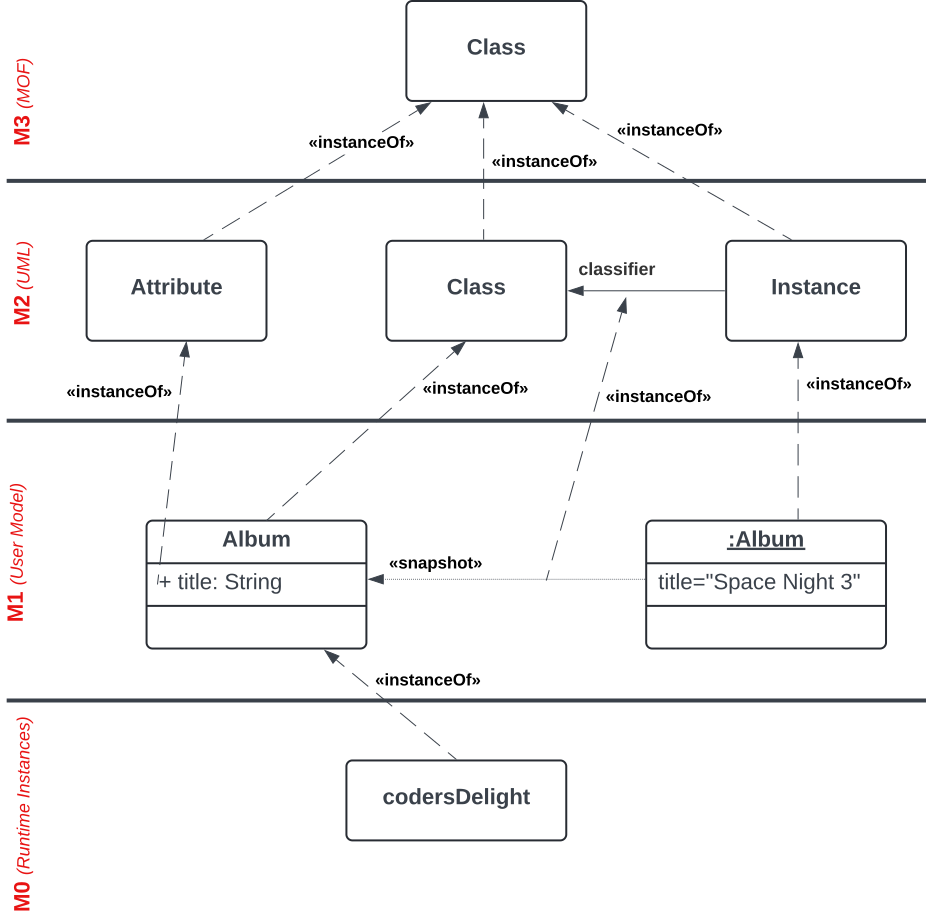
\includegraphics[scale=0.4]{part three/Einführung/img/metamodel}
    \caption{Beispiel für die verschiedenen Schichten der Metamodell Hierarchie.
        In der original Abbildung sind die Pfeilspitzen offen. (Quelle: in Anlehnung an S. 20, Figure 7.8, \url{https://www.omg.org/spec/UML/2.4.1/Infrastructure/PDF}, abgerufen 01.05.2024}
    \label{fig:metamodel-cc}
\end{figure}

\clearpage


\section{Strukturdiagramme}

\begin{tcolorbox}[title=Strukturdiagramme]
    In den \textbf{Strukturdiagrammen} werden \textbf{statische Strukturaspekte} eines Systems betrachtet.
    Für eine Systemmodellierung können alle dieser 6 Diagramme verwendet werden.

    \begin{itemize}
        \item \textbf{Klassendiagramm}: Das \textbf{Klassendiagramm} wird verwendet, um ein objektorientiertes System zu beschreiben.
        \item \textbf{Paketdiagramm}: Ein \textbf{Paketdiagramm} zeigt die Pakete eines Systems und deren Beziehungen.
        \item \textbf{Komponentendiagramm}: Stellt Komponenten oder auch \textit{Subsysteme} mit definierten Interfaces dar, um bspw. \textbf{Architekturdesign} darzustellen.
        \item \textbf{Verteilungsdiagramm}: Beschreibt eine Menge von Knoten, die die \textit{Ausführungsarchitektur} eines Systems definieren können, wobei Knoten i.d.R. \textit{Geräte} oder \textit{Softwareablaufumgebungen repräsentieren}.
        \item \textbf{Kompositionsstrukturdiagramm}: Stellt die \textbf{Komposition} von \textit{Systemstrukturen} (Klassen, Komponenten, Gesamtsystem) in einem bestimmten \textit{Kontext} mit einem bestimmten \textit{Ziel} dar (vgl. \cite[9]{Buh09}).
        \item \textbf{Objektdiagramm}: Momentaufnahme eines Systems zu genau einem \textit{Zeitpukt} während der Ausführung
    \end{itemize}

\end{tcolorbox}
\clearpage

\section{Verhaltensdiagramme}

\begin{tcolorbox}[title=Verhaltensdiagramme]
    \textbf{Verhaltensdiagramme} stellen \textit{Dynamik}, \textit{interne Abläufe} und das \textit{Zusammenspiel} der Systemteile dar, um eine Spezifikation zu vervollständigen.

    \begin{itemize}
        \item \textbf{Anwendungsfalldiagramm}: Dienen zur \textit{Spezifizierung} und \textit{Formalisierung} von \textit{Systemanforderungen}, unter Berücksichtigung von \textbf{Akteuren}, \textbf{Systemen} und \textbf{Anwendungsfällen}
        \item \textbf{Zustandsdiagramm}: Auch \textbf{Zustandsautomaten}; zeigen für ein einzelnes Objekt Zustandsänderungen während der Lebenszeit
        \item \textbf{Aktivitätsdiagramme}: Werden zur Modellierung von \textit{Kontroll}- oder \textit{Objektflüssen} oder zur Darstellung von \textit{Programmlogik} genutzt.
        \item \textbf{Interaktionsdiagramme}: Stellen das Zusammenspiel mehrerer Kommunikationspartner dar.
        Es gibt unterschiedliche Typen von Interaktionsdiagrammen, die Interaktionen auf verschiedenen \textit{Abstraktionsebenen} modellieren:
        \begin{itemize}
            \item \textbf{Sequenzdiagramm}: Zeigt den Verlauf einer Interaktion in zwei Dimensionen, \textit{Kommunikationspartner} und die Nachrichten in ihrer \textit{zeitlichen Abfolge}
            \item \textbf{Kommunikationsdiagramm}: hebt die Kommunikationsbeziehungen zwischen den Partnern hervor
            \item \textbf{Timing Diagramm}: hebt die zeitlichen Aspekte einer Interaktion hervor
            \item \textbf{Interaktionsüberblickdiagramm}: Spezialfall des \textbf{Aktivitätsdiagramms} - statt Aktionen und Aktivitäten können das \textbf{Sequenz}-, \textbf{Kommunikations}- und das \textbf{Timing}-Diagramm als Knoten verwendet werden.
        \end{itemize}
        Alle verwenden dieselben Grundelemente: \textit{Lebenslinien} der Akteure und Nachrichten, die zwischen diesen ausgetauscht werden.
    \end{itemize}
\end{tcolorbox}

\clearpage


\section{Klassendiagramm}

\begin{tcolorbox}[title=Klassendiagramm]
    Das \textbf{Klassendiagramm} beschreibt die Klassen eines Systems und die statischen Beziehungen zwischen ihnen.\\
    Sie werden in Form von Domainklassen bei der \textbf{Analyse} und als detaillierte Entwürfe von Systemklassen als \textit{Blueprint} im \textbf{gesamten Entwicklungsprozess} eingesetzt.

\end{tcolorbox}
\clearpage


\section{Assoziationsklasse (Attributierte Assoziation)}

\begin{tcolorbox}[title=Assoziationsklasse (Attributierte Assoziation)]
Eine \textbf{Assoziationsklasse} erlaubt das Hinzufügen von Operationen und Attributen zu einer Assoziation (\cite[43]{Buh09}).\\
Assoziationsklassen werden in der \textbf{Analyse} in Modellen verwendet und in dem \textbf{Entwurf} in eigenständige Klassen transformiert.\\

\noindent
Assoziationsklassen werden in der \textbf{Analyse} in Modellen verwendet und in dem \textbf{Entwurf} in eigenständige Klassen transformiert.

\blockquote[{\cite[277]{Oes05}}]{
    Eine attributierte Assoziation ist immer dann nahe liegend, wenn Attribute oder Operationen gefunden werden, die weder der einen noch der anderen Klasse zugeordnet werden können, weil sie nämlich Eigenschaften der Beziehung selbst sind.
}.\\

Bei einer attributierten Assoziation dürfen zwei beteiligte Objekte maximal nur eine Beziehung zueinander haben (vgl.~\cite[277]{Oes05})\footnote{
    \textit{Ostereich} führt dies ebenda auf Seite 278 weiter aus, in dem er beschreibt, wie eine attributierte Assoziation für ein \textit{Beschäftigtenverhältnis} zwischen \textit{Mitarbeiter} und \textit{Unternehmen} modelliert wird. Dabei wird davon ausgegangen, dass ein \textit{Mitarbeiter} nur über \textit{ein} Arbeitsverhältnis mit einem \textit{Unternehmen} in Beziehung stehen kann. Bestehen mehrere Arbeitsverhältnisse (\textit{Mitarbeiter} hat zu unterschiedlichen Zeitpunkten für das \textit{Unternehmen} gearbeitet), kann die attributierte Assoziation nicht verwendet werden.\\

\noindent
Wird eine attributierte Assoziation in eine gewöhnliche Assoziation transformiert, muss darauf geachtet werden, die Multiplizitäten richtig zu setzen (s. Abbildung~\ref{fig:assoziationsklasse}).
\end{tcolorbox}

\begin{figure}
    \centering
    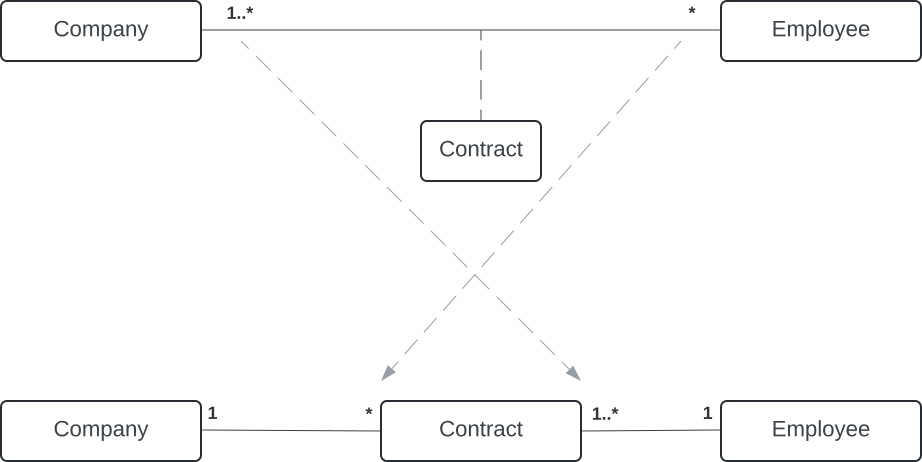
\includegraphics[scale=0.4]{part three/Klassendiagramme - Erweiterte Konzepte und Paketdiagramme/img/assoziationsklasse}
    \caption{Darstellung einer Assoziation mit Hilfe einer Assoziationsklasse (oben) sowie Transformation in gewöhnliche Assoziationen (unten). (Quelle: in Anlehnung an \cite[279, Abb. 4.4-11]{Oes05})}
    \label{fig:assoziationsklasse-cc}
\end{figure}

\clearpage


\section{Sequenzdiagramme}

\begin{tcolorbox}[title=Sequenzdiagramme]
    \textbf{Sequenzdiagramme} stellen Verhalten auf der Ebene einer Interaktion dar.\\
    In der Phase des Klassendesigns werden die Teilnehmer der Interaktionen bestimmt, weshalb Sequenzdiagramme oft in dieser Phase genutzt werden.\\
    In der \textbf{Analysephase} können Sequenzdiagramme eingesetzt werden, um die Kommunikation der bis dahin ausgemachten \textbf{Geschäftsobjekte} zu modellieren, oder um \textbf{Anwendungsfälle} weiter zu spezifizieren.
\end{tcolorbox}
\clearpage

\section{Aggregation}

\begin{tcolorbox}[title=Aggregation]
    Eine \textbf{Aggregation} ist in ihrer \semantischen Aussage unscharf (vgl.~\cite[40]{Buh09}).\\
    Sie beschreibt eine \textit{Ganzes}-\textit{Teile}-Beziehung, aber die \textit{Teile} können zu mehreren verschiedenen \textit{Ganzen} gehören.\\
    Außerdem kann ein Teil dem \textit{Ganzen} jederzeit wieder entnommen werden und das \textit{Ganze} ist nicht verantwortlich für das Erstellen der \textit{Teile}, weshalb Implementierungen beim Hinzufügen von Teilen oft schon fertige Objekte erwarten, die jeweils eines der \textit{Teile} repräsentieren.\\
    Aggregationsbeziehungen werden durch eine nicht-gefüllte Raute an der Seite der Klasse, die das Ganze repräsentiert, dargestellt.
\end{tcolorbox}
\clearpage

\section{Komposition}

\begin{tcolorbox}[title=Komposition]
    Bei einer \textbf{Komposition} handelt es sich um eine \textit{Ganzes}-\textit{Teile}-Beziehung, bei der das \textit{Ganze} verantwortlich für die Erstellung und Beseitigung der \textit{Teile} ist.
    Außerdem sind die \textit{Teile} an die \textbf{Existenz} des \textit{Ganzen} gebunden.\\
    \textit{Teile} gehören immer zu \textit{genau einem} \textit{Ganzen}.\\
    Eine Komposition wird dargestellt durch eine gefüllte Raute an der Klassenbox, die das \textit{Ganze} repräsentiert.
\end{tcolorbox}
\clearpage

\section{Paketdiagramm}

\begin{tcolorbox}[title=Komposition]
    \textbf{Paketdiagramme} zeigen Pakete und ihre Abhängigkeiten und werden in frühen Designphasen genutzt, um Strukturen (großer Systeme) aufzuzeigen.\\

    \noindent
    Elemente sollten so in Paketen gruppiert werden, dass ihr \textbf{funktionaler Zusammenhalt} (\textit{Kohäsion}, s. Abschnitt~\ref{subsec:hohe-kohasion}) klar wird.\\
    Hierdurch kann vermieden werden, dass Änderungen einer Klasse eines Paketes auch Änderungen außerhalb des Paketes erfordern.\\
    Außerdem erhöht sich die Wahrscheinlichkeit, dass einzelne Pakete als solche in anderen Projekten wiederverwendet werden können.\\

    \noindent
    In Paketdiagrammen können Beziehungen über folgende Schlüsselwörter deutlich gemacht werden:

    \begin{itemize}
        \item \guillemotleft import\guillemotright
        \item[] $\rightarrow$ \textbf{public-Import} zwischen Quell- und Zielpaket; Quellpaket kann die öffentlichen Elemente des Zielpaketes unter Verwendung des unqualifizierten und des qualifizierten Namens verwenden; die importierten Elemente sind auch für Pakete sichtbar, die das Quellpaket importieren
        \item \guillemotleft access\guillemotright
        \item[] $\rightarrow$ \textbf{privater Import} zwischen Quell- und Zielpaket; Zugriff auf Elemente des importierten Paketes ohne qualifizierenden Namen möglich; der Import eines Paketes in \textbf{Java} entspricht der \guillemotleft access\guillemotright-Beziehung
        \item \guillemotleft merge\guillemotright
        \item[] $\rightarrow$ Bei einem \textbf{merge} werden Elemente eines Zielpaketes in das Quellpaket
   \end{itemize}
\end{tcolorbox}
\clearpage

\section{Anwendungsfalldiagramm}

\begin{tcolorbox}[title=Anwendungsfalldiagramm]
    Die \textbf{Anwendungsfallanalyse} wird im Rahmen der \textbf{Anforderungsspezifikation} eingesetzt.\\

    \noindent
    Anwendungsfalldiagramme sind das am häufigsten eingesetzte Mittel zur Aufnahme und Darstellung von \textbf{Anforderungen}.\\
    Sie beschreiben selbst kein Verhalten und keine Abläufe, sondern zeigen nur die Zusammenhänge der an Anwendungsfällen beteiligten Modellelemente und sind somit ein Hilfsmittel zur Anforderungsermittlung und Verwaltung.\\

    \noindent
    Zu den wichtigsten Schritten einer Anwendungsfallanalyse gehören:
    \begin{enumerate}
        \item Akteure identifizieren
        \item Anwendungsfälle identifizieren
        \item Beschreiben der Akteure und Anwendungsfälle
        \item Identifizieren von \textit{Schlüsselobjekten}, die das System verwaltet
        \item Identifizieren der wichtigsten Anwendungsfälle (Priorisierung)
        \item detailliertere Beschreibung der Anwendungsfälle
        \item Strukturierung des Anwendungsfalldiagramms
    \end{enumerate}

    \noindent
    Anwendungsfälle beschreiben das \textbf{Szenario} der Nutzung, und nicht Features des Systems.
\end{tcolorbox}

\clearpage

\input{chapters/Anhang/CheatSheets/SE3/Aktivitätsdiagramm}
\clearpage

\section{Zustandsautomat}

\begin{tcolorbox}[title=Zustandsautomat]
    Mit \textbf{Zustandsautomaten} kann das \textit{Verhalten} von Systemen modelliert werden, wobei die \textit{Reaktionen} des Systems im Mittelpunkt stehen, und nicht die \textit{Aktionen}, wie bspw. bei den \textbf{Aktivitätsdiagrammen}.\\

    \noindent
        Ein \textbf{Zustandsautomat} kann den \textit{Lebensweg} eines Objektes modellieren, weshalb Zustandsautomaten oft im \textbf{Entwurf} als Ergänzung zu den \textbf{Klassendiagrammen} eingesetzt werden.
\end{tcolorbox}

\begin{figure}
    \centering
    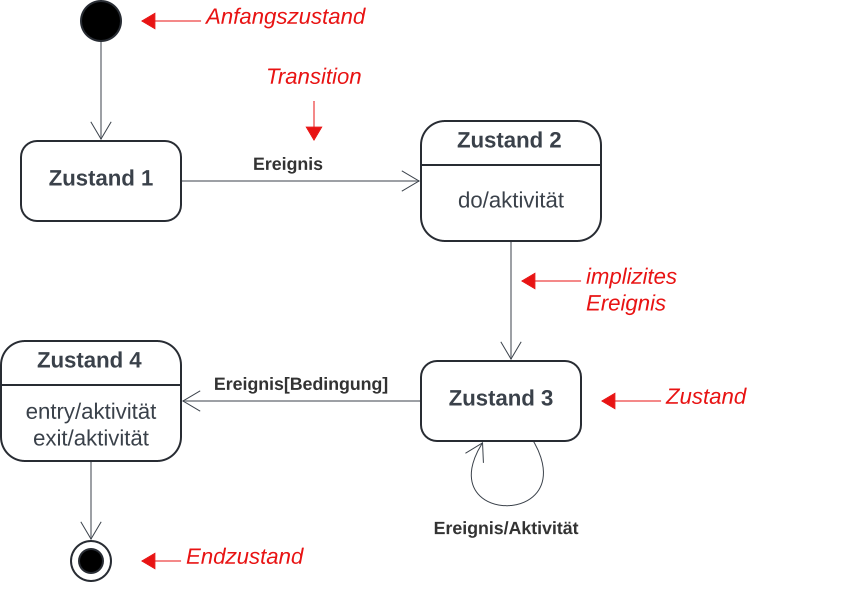
\includegraphics[scale=0.4]{part three/Zustandsautomaten/img/statechartdiagramnotation}
    \caption{Elemente eines einfachen Zustandsautomaten. Eine Transitionen wird durch ein \textbf{Ereignis} ausgelöst, das ein \textit{Signal}, ein \textit{Operationsaufruf} oder auch eine bestimmte \textit{Attributänderung} sein kann. (Quelle: in Anlehnung an \cite[90, Abb. 2.11-6]{Bal05})}
    \label{fig:statechartdiagramnotation-cc}
\end{figure}

\begin{minted}[fontsize=\small]{java}
// Beispiel für eine Implementierung eines
// Parkscheinautomaten als Zustandsautomat in Java
class Parkscheinautomat {

  // zustände
  private final int BEREIT = 0;
  private final int ZAHLUNG = 1;
  private final int ABBRUCH = 2;
  private final int BELEG   = 3;

  // Zustand; wird initial beim Starten
  // des Automaten gesetzt
  private int zustand;

  // Methoden lösen Aktionen beim Eintritt
  // in die jeweiligen Zustände aus
  private int zahlung() {
    // verarbeiten
    // danach neuen Zustand zurückliefern...
    ...
    return BEREIT;
  }

   ...

  private void bereit() {
    while (true) {
      // eingabe überprüfen und
      // ggf. Zustandswechsel auslösen:
      // Zustand als Attribut setzen
      ...
    }
  }

  public void start() {
    zustand = BEREIT;

    while(true) {
      switch (zustand) {
        case BEREIT:
          zustand = bereit();
        // ... weiteres Verhalten
        ...
      }
    }
  }
}
\end{minted}
\clearpage
	

\section{Inhalt SE3}

\section*{1. Übersicht UML}

\subsection*{Lernziele}
\begin{itemize}
    \item einen Einblick in den Sprachaufbau der UML 2.0 gewinnen
    \item einen Überblick über die Diagramme der UML 2.0 und deren Zweck haben
\end{itemize}

\subsection*{Zusammenfassung}
\begin{itemize}
    \item Die \textbf{UML} ist eine weit verbreitete Modellierungssprache zur Modellierung objektorientierter Softwaresysteme.
    \item Die UML 2.0 Spezifikation besteht aus vier Teilen:
    \begin{enumerate}
        \item \textbf{Superstructure}: Diagrammtypen
        \item \textbf{Infrastructure}: Modellierungskonzepte
        \item \textbf{OCL}: formale Sprache zur Formulierung von Einschränkungen
        \item \textbf{Diagram Interchange}: Austauschformate
    \end{enumerate}
    \item Die UML kann im \textbf{Sketching} oder \textbf{Blueprint Modus} eingesetzt werden, oder als Grundlage für \textbf{automatische Codegenerierung}
    \item Die UML ist an keinen speziellen Entwicklungsprozess gebunden
\end{itemize}

\section*{2. Klassendiagramme}

\subsection*{Lernziele}
\begin{itemize}
    \item wissen, wie Klassendiagramme im Entwicklungsprozess eingesetzt werden
    \item Klassendiagramme für Analyse- und Designentscheidungen einsetzen können
    \item die wichtigsten Modellierungskonzepte kennen
    \item sinnvolle Klassendiagramme erstellen und Java-Implementierungen ableiten können
    \item Klassendiagramme aus Java Quellcode erzeugen können
\end{itemize}

\subsection*{Zusammenfassung}

\begin{itemize}
    \item \textbf{Klassendiagramme} dienen zur \textbf{strukturellen Darstellung} von Softwaresystemen
    \item hierbei werden Klassen und \textbf{Beziehungen} zwischen Klassen dargestellt
    \item Properties können durch die \textbf{Attribut}- oder \textbf{Assoziationsnotation} modelliert werden
    \item Operationen werden als separate Zeile in ihrem Compartment dargestellt
    \item im Klassendiagramm können auch \textbf{Generalisierungsbeziehungen} modelliert werden
    \item \textbf{Abhängigkeitsbeziehungen} drücken ein Verhältnis zwischen \textbf{Client} und \textbf{Supplier} aus
\end{itemize}

\section*{3. Objektorientierter Entwurf}

\subsection*{Lernziele}
\begin{itemize}
    \item das Wesen einer Interaktion kennen
    \item wissen, wie Sequenzdiagramme im Entwicklungsprozess eingesetzt werden
    \item Sequenzdiagramme für Analyse- und Designentscheidungen sowie zur Darstellung von Kontrollflüssen einsetzen können
    \item die wichtigsten Modellierungskonzepte kennen
    \item sinnvolle Sequenzdiagramme erstellen und Java-Implementierungen ableiten können
    \item Sequenzdiagramme aus Java Quellcode erzeugen können
\end{itemize}

\subsection*{Zusammenfassung}

\begin{itemize}
    \item Sequenzdiagramme sind \textbf{Verhaltensdiagramme}
    und können im gesamten Entwicklungszyklus zur Modellierung von Interaktionen angewendet werden
    \item Interaktionen bestehen im Wesentlichen aus dem Nachrichtenaustausch zwischen verschiedenen Kommunikationspartnern
    \item in den meisten Fällen wird die Kommunikation von Objekten von Klassen modelliert, aber es können auch Teilnehmer auf anderen Ebenen modelliert werden
    \item gewöhnlich gibt ein Sequenzdiagramm einen \textbf{Anwendungsfall} (\textit{Szenario}) wieder
    \item sie dienen nicht dazu, um Zustandsänderungen darzustellen (hierfür werden Zustandsdiagramme verwendet)
    \item Sequenzdiagramme sind \textit{nicht} gut geeignet für die Darstellung von
    \begin{itemize}
        \item nebenläufigem Verhalten (\textit{asynchrone} Nachrichten, \textit{kombiniertes Fragment})
        \item Schleifen und alternativem Verhalten (\textit{kombinierte Fragmente})
        \item[] $\rightarrow$  für beide Fälle sind \textbf{Aktivitätsdiagramme} besser geeignet
    \end{itemize}
\end{itemize}

\section*{4. Klassendiagramme - Erweiterte Konzepte und Paketdiagramme}

\subsection*{Lernziele}
\begin{itemize}
    \item erweiterte Modellierungskonzepte in Klassendiagrammen für den Detailentwurf von Systemen kennen
    \item die Konsequenzen dieser Konzepte in der Implementierung kennen
    \item wissen, wie Paketdiagramme im Entwicklungsprozess eingesetzt werden
    \item die Modellierungskonzepte in Paketdiagrammen kennen
    \item anhand von Paketdiagrammen Software-Architekturen gestalten und bewerten können
\end{itemize}

\subsection*{Zusammenfassung}

\begin{itemize}
    \item Die vorgestellten erweiterten Konzepte werden vor allem im \textbf{Feinentwurf} von Klassenstrukturen eingesetzt.
    \item Generell gilt, dass die Spezifikationen von Objekten und Properties nur so detailliert ausgeführt werden sollen, wie nötig: Sind Details für das Verständnis unnötig, sollte darauf verzichtet werden.
    \item \textbf{Generalisierungsbeziehungen} sollten grundsätzlich modelliert werden.
    \item Ist eine \textbf{Komposition} statt einer Generalisierung für den Sachverhalt möglich, sollte diese verwendet werden: ``Favor object composition over inheritance.`` (\cite[19 f.]{GHJV94})
    \item \textbf{Kompositionsbeziehungen} geben eindeutige Impulse für eine Implementierung, \textbf{Aggregationsbeziehungen} sind in ihrer semantischen Aussage nicht sehr eindeutig
    \item \textbf{Assoziationsklassen} sind in ihrer frühen Designphase empfehlenswert, die Realisierung (mit {bspw.} Java) erfordert aber eine Transformation in eine volle Klasse, wobei die Multiplizitäten angepasst werden müssen
    \item Elemente können in \textbf{Paketen} zusamengefasst und unter einem gemeinsamen Namensraum gruppiert werden
\end{itemize}

\section*{4. Anwendungsfalldiagramm (Use-Case-Diagramm)}

\subsection*{Lernziele}
\begin{itemize}
    \item wissen, wie die Anwendungsfallanalyse im Rahmen der Anforderungsspezifikation eingesetzt wird
    \item Prozessschritte der Anwendungsfallanalyse beherrschen
    \item die wichtigsten Modellierungskonzepte in Anwendungsfalldiagrammen kennen
    \item den Aufbau einer Anwendungsfallbeschreibung kennen
\end{itemize}

\subsection*{Zusammenfassung}

\begin{itemize}
    \item \textbf{Anwendungsfalldiagramme} besitzen eine einfache Notation, um \textbf{Akteure} und \textbf{Anwendungsfälle} eines \textbf{Systems} grafisch darzustellen
    \item auf Basis eines Anwendungsfalldiagramms lässt sich ermitteln, ob die Anwendungsfälle gewünschtes Verhalten realisieren bzw. Beziehungen zu einem oder mehreren Akteuren haben
    \item Anwendungsfälle und Akteure \textit{müssen} zusätzlich textlich beschrieben werden
\end{itemize}

\section*{5. Aktivitätsdiagramme}

\subsection*{Lernziele}
\begin{itemize}
    \item wissen, wie Aktivitätsdiagramme im Rahmen der Verhaltensanalyse in verschiedenen Prozessphasen eingesetzt werden können
    \item die wichtigsten Modellierungskonzepte in Aktivitätsdiagrammen kennen
    \item Aktivitätsdiagramme interpretieren, erstellen und implementieren können
\end{itemize}

\subsection*{Zusammenfassung}

\begin{itemize}
    \item \textbf{Aktivitätsdiagramme} gehören zu den \textbf{Verhaltensdiagrammen} und können im \textit{gesamten} \textbf{Entwicklungsprozess} eingesetzt werden
    \item durch ein Aktivitätsdiagramm kann gezeigt werden, wie \textbf{Verhalten} realisiert wird
    \item es können mehrere \textbf{Aktivitäten} dargestellt werden
    \item \textbf{Aktivitätskanten} und \textbf{Aktivitätsknoten} werden zur Beschreibung von Verhalten verwendet
\end{itemize}

\section*{5. Zustandsautomaten}

\subsection*{Lernziele}
\begin{itemize}
    \item wissen, wie Zustandsdiagramme im Rahmen der Verhaltensanalyse einzelner Objekte eingesetzt werden können
    \item die wichtigsten Modellierungskonzepte in Zustandsdiagrammen kennen
    \item Zustandsdiagramme interpretieren, erstellen und implementieren können
\end{itemize}

\subsection*{Zusammenfassung}

\begin{itemize}
    \item Das \textbf{Zustandsdiagramm} gehört wie das \textbf{Aktivitätsdiagramm} zu den \textbf{Verhaltensdiagrammen}.
    \item Ein Zustandsdiagramm zeigt den \textbf{Lebensweg} eines \textbf{Objektes}.
    \item \textbf{Attributwerte} bestimmen den Zustand eines Objektes.
    \item \textbf{Transitionen} zwischen Zuständen werden durch \textbf{Guards} und \textbf{Events} gesteuert.
    \item Während der Transitionen können \textbf{Effekte} (\textit{Aktivitäten}) realisiert werden.
    \item Die Modellierung \textbf{zusammengesetzter Zustände} ist ebenfalls möglich.
    \item Für die Darstellung \textbf{paralleler} oder  \textbf{konkurrierender} Abläufe können \textbf{Regionen} modelliert werden.
\end{itemize}
\clearpage


\section{UML Modellierung}

\begin{tcolorbox}[title=UML Modellierung]
    \textbf{Modelle} haben die Aufgabe, den Bezug zum Original (Programm, Softwaresystem) herzustellen, sowie zu der \textit{Anwendungsumgebung}.\\
    Ein \textbf{Modell} enthält alle \textbf{Modellelemente}, die zur Beschreibung eines Softwaresystems nötig sind.\\

    \noindent
    Ein \textbf{Modellelement} wird als Element in einem UML Modell von einem Benutzer erstellt und auf verschiedenen \textbf{Diagrammen} (Struktur-/Verhaltensdiagrammen) platziert, und wird durch die \textbf{UML Modellierungskonzepte} als Metaklasse des \textbf{Metamodells} der UML beschrieben: \textbf{Modellelemente} werden aus Modellierungskonzepten instanziiert.\\

    \noindent
       Das \textbf{UML Metamodell} regelt, in welchem Zusammenhang \textbf{UML Modellierungskonzepte} in Modellen auftreten dürfen, und welche Eigenschaften und Beziehungen zu anderen Sprachelementen zulässig sind.\\

       \noindent
       Die im \textbf{Metamodell} verwendeten Erklärungen basieren auf einer abstrakten Syntax, für deren Beschreibung eine Untermenge (\textit{Klassendiagramme}) der UML verwendet wird.\\
        Die \textbf{Semantik} der Modellierungskonzepte wird textlich beschrieben, zur Formalisierung von Regeln für die syntaktische Korrektheit wird die \textbf{OCL} (\textit{Object Constraint Language}) verwendet.
\end{tcolorbox}

\begin{figure}
    \centering
    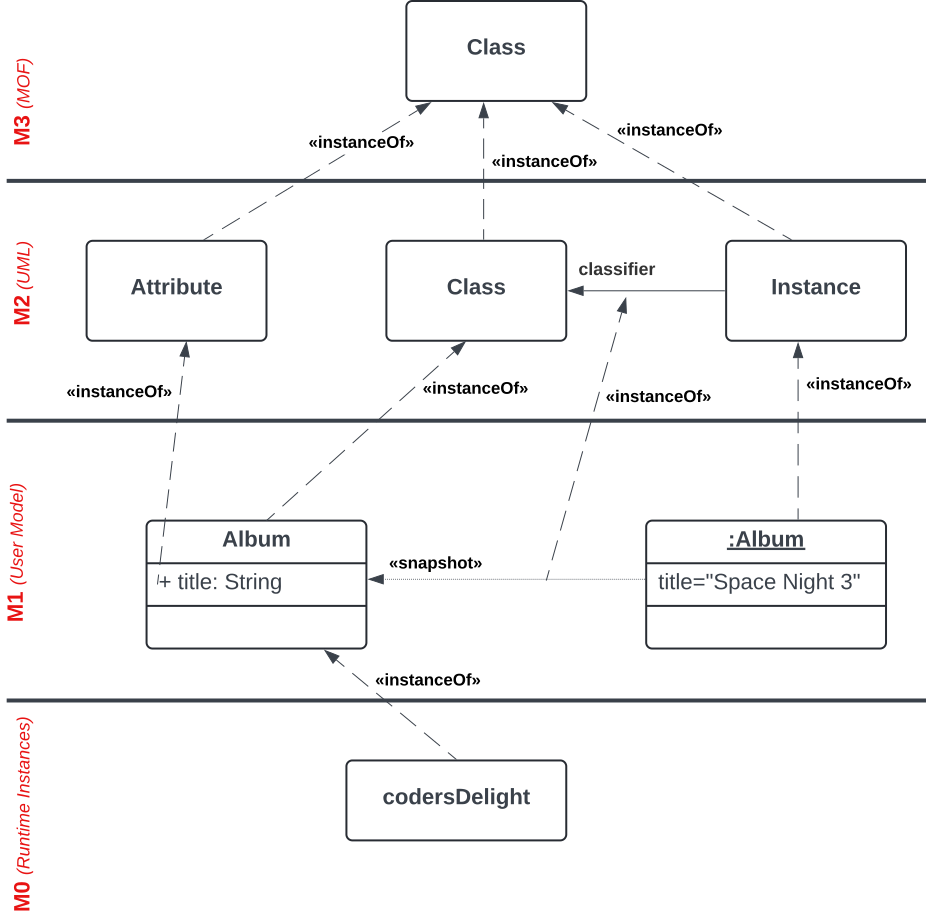
\includegraphics[scale=0.4]{part three/Einführung/img/metamodel}
    \caption{Beispiel für die verschiedenen Schichten der Metamodell Hierarchie.
        In der original Abbildung sind die Pfeilspitzen offen. (Quelle: in Anlehnung an S. 20, Figure 7.8, \url{https://www.omg.org/spec/UML/2.4.1/Infrastructure/PDF}, abgerufen 01.05.2024}
    \label{fig:metamodel-cc}
\end{figure}

\clearpage


\section{Strukturdiagramme}

\begin{tcolorbox}[title=Strukturdiagramme]
    In den \textbf{Strukturdiagrammen} werden \textbf{statische Strukturaspekte} eines Systems betrachtet.
    Für eine Systemmodellierung können alle dieser 6 Diagramme verwendet werden.

    \begin{itemize}
        \item \textbf{Klassendiagramm}: Das \textbf{Klassendiagramm} wird verwendet, um ein objektorientiertes System zu beschreiben.
        \item \textbf{Paketdiagramm}: Ein \textbf{Paketdiagramm} zeigt die Pakete eines Systems und deren Beziehungen.
        \item \textbf{Komponentendiagramm}: Stellt Komponenten oder auch \textit{Subsysteme} mit definierten Interfaces dar, um bspw. \textbf{Architekturdesign} darzustellen.
        \item \textbf{Verteilungsdiagramm}: Beschreibt eine Menge von Knoten, die die \textit{Ausführungsarchitektur} eines Systems definieren können, wobei Knoten i.d.R. \textit{Geräte} oder \textit{Softwareablaufumgebungen repräsentieren}.
        \item \textbf{Kompositionsstrukturdiagramm}: Stellt die \textbf{Komposition} von \textit{Systemstrukturen} (Klassen, Komponenten, Gesamtsystem) in einem bestimmten \textit{Kontext} mit einem bestimmten \textit{Ziel} dar (vgl. \cite[9]{Buh09}).
        \item \textbf{Objektdiagramm}: Momentaufnahme eines Systems zu genau einem \textit{Zeitpukt} während der Ausführung
    \end{itemize}

\end{tcolorbox}
\clearpage

\section{Verhaltensdiagramme}

\begin{tcolorbox}[title=Verhaltensdiagramme]
    \textbf{Verhaltensdiagramme} stellen \textit{Dynamik}, \textit{interne Abläufe} und das \textit{Zusammenspiel} der Systemteile dar, um eine Spezifikation zu vervollständigen.

    \begin{itemize}
        \item \textbf{Anwendungsfalldiagramm}: Dienen zur \textit{Spezifizierung} und \textit{Formalisierung} von \textit{Systemanforderungen}, unter Berücksichtigung von \textbf{Akteuren}, \textbf{Systemen} und \textbf{Anwendungsfällen}
        \item \textbf{Zustandsdiagramm}: Auch \textbf{Zustandsautomaten}; zeigen für ein einzelnes Objekt Zustandsänderungen während der Lebenszeit
        \item \textbf{Aktivitätsdiagramme}: Werden zur Modellierung von \textit{Kontroll}- oder \textit{Objektflüssen} oder zur Darstellung von \textit{Programmlogik} genutzt.
        \item \textbf{Interaktionsdiagramme}: Stellen das Zusammenspiel mehrerer Kommunikationspartner dar.
        Es gibt unterschiedliche Typen von Interaktionsdiagrammen, die Interaktionen auf verschiedenen \textit{Abstraktionsebenen} modellieren:
        \begin{itemize}
            \item \textbf{Sequenzdiagramm}: Zeigt den Verlauf einer Interaktion in zwei Dimensionen, \textit{Kommunikationspartner} und die Nachrichten in ihrer \textit{zeitlichen Abfolge}
            \item \textbf{Kommunikationsdiagramm}: hebt die Kommunikationsbeziehungen zwischen den Partnern hervor
            \item \textbf{Timing Diagramm}: hebt die zeitlichen Aspekte einer Interaktion hervor
            \item \textbf{Interaktionsüberblickdiagramm}: Spezialfall des \textbf{Aktivitätsdiagramms} - statt Aktionen und Aktivitäten können das \textbf{Sequenz}-, \textbf{Kommunikations}- und das \textbf{Timing}-Diagramm als Knoten verwendet werden.
        \end{itemize}
        Alle verwenden dieselben Grundelemente: \textit{Lebenslinien} der Akteure und Nachrichten, die zwischen diesen ausgetauscht werden.
    \end{itemize}
\end{tcolorbox}

\clearpage


\section{Klassendiagramm}

\begin{tcolorbox}[title=Klassendiagramm]
    Das \textbf{Klassendiagramm} beschreibt die Klassen eines Systems und die statischen Beziehungen zwischen ihnen.\\
    Sie werden in Form von Domainklassen bei der \textbf{Analyse} und als detaillierte Entwürfe von Systemklassen als \textit{Blueprint} im \textbf{gesamten Entwicklungsprozess} eingesetzt.

\end{tcolorbox}
\clearpage


\section{Assoziationsklasse (Attributierte Assoziation)}

\begin{tcolorbox}[title=Assoziationsklasse (Attributierte Assoziation)]
Eine \textbf{Assoziationsklasse} erlaubt das Hinzufügen von Operationen und Attributen zu einer Assoziation (\cite[43]{Buh09}).\\
Assoziationsklassen werden in der \textbf{Analyse} in Modellen verwendet und in dem \textbf{Entwurf} in eigenständige Klassen transformiert.\\

\noindent
Assoziationsklassen werden in der \textbf{Analyse} in Modellen verwendet und in dem \textbf{Entwurf} in eigenständige Klassen transformiert.

\blockquote[{\cite[277]{Oes05}}]{
    Eine attributierte Assoziation ist immer dann nahe liegend, wenn Attribute oder Operationen gefunden werden, die weder der einen noch der anderen Klasse zugeordnet werden können, weil sie nämlich Eigenschaften der Beziehung selbst sind.
}.\\

Bei einer attributierten Assoziation dürfen zwei beteiligte Objekte maximal nur eine Beziehung zueinander haben (vgl.~\cite[277]{Oes05})\footnote{
    \textit{Ostereich} führt dies ebenda auf Seite 278 weiter aus, in dem er beschreibt, wie eine attributierte Assoziation für ein \textit{Beschäftigtenverhältnis} zwischen \textit{Mitarbeiter} und \textit{Unternehmen} modelliert wird. Dabei wird davon ausgegangen, dass ein \textit{Mitarbeiter} nur über \textit{ein} Arbeitsverhältnis mit einem \textit{Unternehmen} in Beziehung stehen kann. Bestehen mehrere Arbeitsverhältnisse (\textit{Mitarbeiter} hat zu unterschiedlichen Zeitpunkten für das \textit{Unternehmen} gearbeitet), kann die attributierte Assoziation nicht verwendet werden.\\

\noindent
Wird eine attributierte Assoziation in eine gewöhnliche Assoziation transformiert, muss darauf geachtet werden, die Multiplizitäten richtig zu setzen (s. Abbildung~\ref{fig:assoziationsklasse}).
\end{tcolorbox}

\begin{figure}
    \centering
    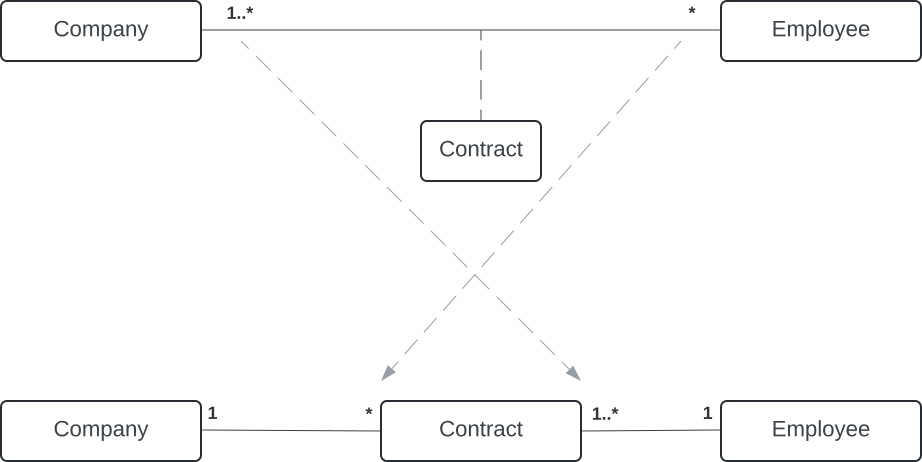
\includegraphics[scale=0.4]{part three/Klassendiagramme - Erweiterte Konzepte und Paketdiagramme/img/assoziationsklasse}
    \caption{Darstellung einer Assoziation mit Hilfe einer Assoziationsklasse (oben) sowie Transformation in gewöhnliche Assoziationen (unten). (Quelle: in Anlehnung an \cite[279, Abb. 4.4-11]{Oes05})}
    \label{fig:assoziationsklasse-cc}
\end{figure}

\clearpage


\section{Sequenzdiagramme}

\begin{tcolorbox}[title=Sequenzdiagramme]
    \textbf{Sequenzdiagramme} stellen Verhalten auf der Ebene einer Interaktion dar.\\
    In der Phase des Klassendesigns werden die Teilnehmer der Interaktionen bestimmt, weshalb Sequenzdiagramme oft in dieser Phase genutzt werden.\\
    In der \textbf{Analysephase} können Sequenzdiagramme eingesetzt werden, um die Kommunikation der bis dahin ausgemachten \textbf{Geschäftsobjekte} zu modellieren, oder um \textbf{Anwendungsfälle} weiter zu spezifizieren.
\end{tcolorbox}
\clearpage

\section{Aggregation}

\begin{tcolorbox}[title=Aggregation]
    Eine \textbf{Aggregation} ist in ihrer \semantischen Aussage unscharf (vgl.~\cite[40]{Buh09}).\\
    Sie beschreibt eine \textit{Ganzes}-\textit{Teile}-Beziehung, aber die \textit{Teile} können zu mehreren verschiedenen \textit{Ganzen} gehören.\\
    Außerdem kann ein Teil dem \textit{Ganzen} jederzeit wieder entnommen werden und das \textit{Ganze} ist nicht verantwortlich für das Erstellen der \textit{Teile}, weshalb Implementierungen beim Hinzufügen von Teilen oft schon fertige Objekte erwarten, die jeweils eines der \textit{Teile} repräsentieren.\\
    Aggregationsbeziehungen werden durch eine nicht-gefüllte Raute an der Seite der Klasse, die das Ganze repräsentiert, dargestellt.
\end{tcolorbox}
\clearpage

\section{Komposition}

\begin{tcolorbox}[title=Komposition]
    Bei einer \textbf{Komposition} handelt es sich um eine \textit{Ganzes}-\textit{Teile}-Beziehung, bei der das \textit{Ganze} verantwortlich für die Erstellung und Beseitigung der \textit{Teile} ist.
    Außerdem sind die \textit{Teile} an die \textbf{Existenz} des \textit{Ganzen} gebunden.\\
    \textit{Teile} gehören immer zu \textit{genau einem} \textit{Ganzen}.\\
    Eine Komposition wird dargestellt durch eine gefüllte Raute an der Klassenbox, die das \textit{Ganze} repräsentiert.
\end{tcolorbox}
\clearpage

\section{Paketdiagramm}

\begin{tcolorbox}[title=Komposition]
    \textbf{Paketdiagramme} zeigen Pakete und ihre Abhängigkeiten und werden in frühen Designphasen genutzt, um Strukturen (großer Systeme) aufzuzeigen.\\

    \noindent
    Elemente sollten so in Paketen gruppiert werden, dass ihr \textbf{funktionaler Zusammenhalt} (\textit{Kohäsion}, s. Abschnitt~\ref{subsec:hohe-kohasion}) klar wird.\\
    Hierdurch kann vermieden werden, dass Änderungen einer Klasse eines Paketes auch Änderungen außerhalb des Paketes erfordern.\\
    Außerdem erhöht sich die Wahrscheinlichkeit, dass einzelne Pakete als solche in anderen Projekten wiederverwendet werden können.\\

    \noindent
    In Paketdiagrammen können Beziehungen über folgende Schlüsselwörter deutlich gemacht werden:

    \begin{itemize}
        \item \guillemotleft import\guillemotright
        \item[] $\rightarrow$ \textbf{public-Import} zwischen Quell- und Zielpaket; Quellpaket kann die öffentlichen Elemente des Zielpaketes unter Verwendung des unqualifizierten und des qualifizierten Namens verwenden; die importierten Elemente sind auch für Pakete sichtbar, die das Quellpaket importieren
        \item \guillemotleft access\guillemotright
        \item[] $\rightarrow$ \textbf{privater Import} zwischen Quell- und Zielpaket; Zugriff auf Elemente des importierten Paketes ohne qualifizierenden Namen möglich; der Import eines Paketes in \textbf{Java} entspricht der \guillemotleft access\guillemotright-Beziehung
        \item \guillemotleft merge\guillemotright
        \item[] $\rightarrow$ Bei einem \textbf{merge} werden Elemente eines Zielpaketes in das Quellpaket
   \end{itemize}
\end{tcolorbox}
\clearpage

\section{Anwendungsfalldiagramm}

\begin{tcolorbox}[title=Anwendungsfalldiagramm]
    Die \textbf{Anwendungsfallanalyse} wird im Rahmen der \textbf{Anforderungsspezifikation} eingesetzt.\\

    \noindent
    Anwendungsfalldiagramme sind das am häufigsten eingesetzte Mittel zur Aufnahme und Darstellung von \textbf{Anforderungen}.\\
    Sie beschreiben selbst kein Verhalten und keine Abläufe, sondern zeigen nur die Zusammenhänge der an Anwendungsfällen beteiligten Modellelemente und sind somit ein Hilfsmittel zur Anforderungsermittlung und Verwaltung.\\

    \noindent
    Zu den wichtigsten Schritten einer Anwendungsfallanalyse gehören:
    \begin{enumerate}
        \item Akteure identifizieren
        \item Anwendungsfälle identifizieren
        \item Beschreiben der Akteure und Anwendungsfälle
        \item Identifizieren von \textit{Schlüsselobjekten}, die das System verwaltet
        \item Identifizieren der wichtigsten Anwendungsfälle (Priorisierung)
        \item detailliertere Beschreibung der Anwendungsfälle
        \item Strukturierung des Anwendungsfalldiagramms
    \end{enumerate}

    \noindent
    Anwendungsfälle beschreiben das \textbf{Szenario} der Nutzung, und nicht Features des Systems.
\end{tcolorbox}

\clearpage

\input{chapters/Anhang/CheatSheets/SE3/Aktivitätsdiagramm}
\clearpage

\section{Zustandsautomat}

\begin{tcolorbox}[title=Zustandsautomat]
    Mit \textbf{Zustandsautomaten} kann das \textit{Verhalten} von Systemen modelliert werden, wobei die \textit{Reaktionen} des Systems im Mittelpunkt stehen, und nicht die \textit{Aktionen}, wie bspw. bei den \textbf{Aktivitätsdiagrammen}.\\

    \noindent
        Ein \textbf{Zustandsautomat} kann den \textit{Lebensweg} eines Objektes modellieren, weshalb Zustandsautomaten oft im \textbf{Entwurf} als Ergänzung zu den \textbf{Klassendiagrammen} eingesetzt werden.
\end{tcolorbox}

\begin{figure}
    \centering
    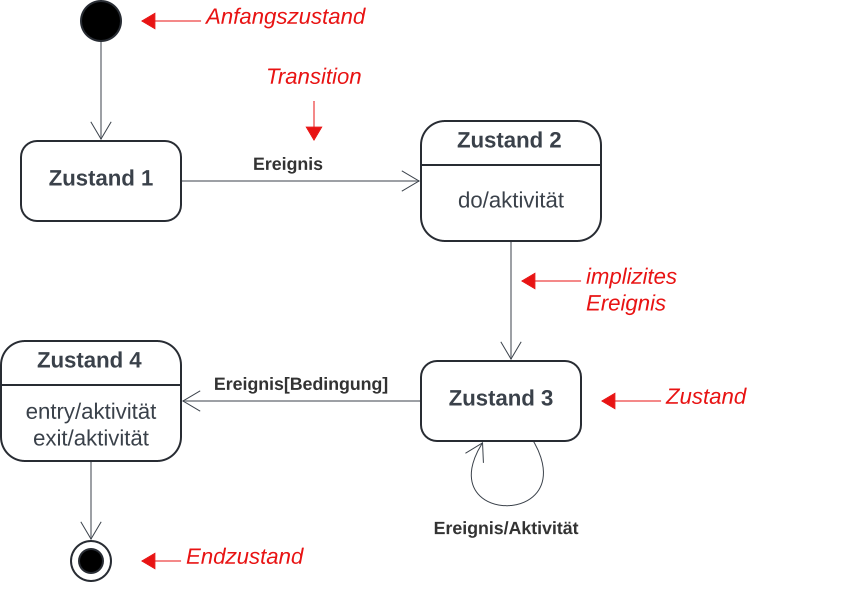
\includegraphics[scale=0.4]{part three/Zustandsautomaten/img/statechartdiagramnotation}
    \caption{Elemente eines einfachen Zustandsautomaten. Eine Transitionen wird durch ein \textbf{Ereignis} ausgelöst, das ein \textit{Signal}, ein \textit{Operationsaufruf} oder auch eine bestimmte \textit{Attributänderung} sein kann. (Quelle: in Anlehnung an \cite[90, Abb. 2.11-6]{Bal05})}
    \label{fig:statechartdiagramnotation-cc}
\end{figure}

\begin{minted}[fontsize=\small]{java}
// Beispiel für eine Implementierung eines
// Parkscheinautomaten als Zustandsautomat in Java
class Parkscheinautomat {

  // zustände
  private final int BEREIT = 0;
  private final int ZAHLUNG = 1;
  private final int ABBRUCH = 2;
  private final int BELEG   = 3;

  // Zustand; wird initial beim Starten
  // des Automaten gesetzt
  private int zustand;

  // Methoden lösen Aktionen beim Eintritt
  // in die jeweiligen Zustände aus
  private int zahlung() {
    // verarbeiten
    // danach neuen Zustand zurückliefern...
    ...
    return BEREIT;
  }

   ...

  private void bereit() {
    while (true) {
      // eingabe überprüfen und
      // ggf. Zustandswechsel auslösen:
      // Zustand als Attribut setzen
      ...
    }
  }

  public void start() {
    zustand = BEREIT;

    while(true) {
      switch (zustand) {
        case BEREIT:
          zustand = bereit();
        // ... weiteres Verhalten
        ...
      }
    }
  }
}
\end{minted}
\clearpage
	

\section{Inhalt SE3}

\section*{1. Übersicht UML}

\subsection*{Lernziele}
\begin{itemize}
    \item einen Einblick in den Sprachaufbau der UML 2.0 gewinnen
    \item einen Überblick über die Diagramme der UML 2.0 und deren Zweck haben
\end{itemize}

\subsection*{Zusammenfassung}
\begin{itemize}
    \item Die \textbf{UML} ist eine weit verbreitete Modellierungssprache zur Modellierung objektorientierter Softwaresysteme.
    \item Die UML 2.0 Spezifikation besteht aus vier Teilen:
    \begin{enumerate}
        \item \textbf{Superstructure}: Diagrammtypen
        \item \textbf{Infrastructure}: Modellierungskonzepte
        \item \textbf{OCL}: formale Sprache zur Formulierung von Einschränkungen
        \item \textbf{Diagram Interchange}: Austauschformate
    \end{enumerate}
    \item Die UML kann im \textbf{Sketching} oder \textbf{Blueprint Modus} eingesetzt werden, oder als Grundlage für \textbf{automatische Codegenerierung}
    \item Die UML ist an keinen speziellen Entwicklungsprozess gebunden
\end{itemize}

\section*{2. Klassendiagramme}

\subsection*{Lernziele}
\begin{itemize}
    \item wissen, wie Klassendiagramme im Entwicklungsprozess eingesetzt werden
    \item Klassendiagramme für Analyse- und Designentscheidungen einsetzen können
    \item die wichtigsten Modellierungskonzepte kennen
    \item sinnvolle Klassendiagramme erstellen und Java-Implementierungen ableiten können
    \item Klassendiagramme aus Java Quellcode erzeugen können
\end{itemize}

\subsection*{Zusammenfassung}

\begin{itemize}
    \item \textbf{Klassendiagramme} dienen zur \textbf{strukturellen Darstellung} von Softwaresystemen
    \item hierbei werden Klassen und \textbf{Beziehungen} zwischen Klassen dargestellt
    \item Properties können durch die \textbf{Attribut}- oder \textbf{Assoziationsnotation} modelliert werden
    \item Operationen werden als separate Zeile in ihrem Compartment dargestellt
    \item im Klassendiagramm können auch \textbf{Generalisierungsbeziehungen} modelliert werden
    \item \textbf{Abhängigkeitsbeziehungen} drücken ein Verhältnis zwischen \textbf{Client} und \textbf{Supplier} aus
\end{itemize}

\section*{3. Objektorientierter Entwurf}

\subsection*{Lernziele}
\begin{itemize}
    \item das Wesen einer Interaktion kennen
    \item wissen, wie Sequenzdiagramme im Entwicklungsprozess eingesetzt werden
    \item Sequenzdiagramme für Analyse- und Designentscheidungen sowie zur Darstellung von Kontrollflüssen einsetzen können
    \item die wichtigsten Modellierungskonzepte kennen
    \item sinnvolle Sequenzdiagramme erstellen und Java-Implementierungen ableiten können
    \item Sequenzdiagramme aus Java Quellcode erzeugen können
\end{itemize}

\subsection*{Zusammenfassung}

\begin{itemize}
    \item Sequenzdiagramme sind \textbf{Verhaltensdiagramme}
    und können im gesamten Entwicklungszyklus zur Modellierung von Interaktionen angewendet werden
    \item Interaktionen bestehen im Wesentlichen aus dem Nachrichtenaustausch zwischen verschiedenen Kommunikationspartnern
    \item in den meisten Fällen wird die Kommunikation von Objekten von Klassen modelliert, aber es können auch Teilnehmer auf anderen Ebenen modelliert werden
    \item gewöhnlich gibt ein Sequenzdiagramm einen \textbf{Anwendungsfall} (\textit{Szenario}) wieder
    \item sie dienen nicht dazu, um Zustandsänderungen darzustellen (hierfür werden Zustandsdiagramme verwendet)
    \item Sequenzdiagramme sind \textit{nicht} gut geeignet für die Darstellung von
    \begin{itemize}
        \item nebenläufigem Verhalten (\textit{asynchrone} Nachrichten, \textit{kombiniertes Fragment})
        \item Schleifen und alternativem Verhalten (\textit{kombinierte Fragmente})
        \item[] $\rightarrow$  für beide Fälle sind \textbf{Aktivitätsdiagramme} besser geeignet
    \end{itemize}
\end{itemize}

\section*{4. Klassendiagramme - Erweiterte Konzepte und Paketdiagramme}

\subsection*{Lernziele}
\begin{itemize}
    \item erweiterte Modellierungskonzepte in Klassendiagrammen für den Detailentwurf von Systemen kennen
    \item die Konsequenzen dieser Konzepte in der Implementierung kennen
    \item wissen, wie Paketdiagramme im Entwicklungsprozess eingesetzt werden
    \item die Modellierungskonzepte in Paketdiagrammen kennen
    \item anhand von Paketdiagrammen Software-Architekturen gestalten und bewerten können
\end{itemize}

\subsection*{Zusammenfassung}

\begin{itemize}
    \item Die vorgestellten erweiterten Konzepte werden vor allem im \textbf{Feinentwurf} von Klassenstrukturen eingesetzt.
    \item Generell gilt, dass die Spezifikationen von Objekten und Properties nur so detailliert ausgeführt werden sollen, wie nötig: Sind Details für das Verständnis unnötig, sollte darauf verzichtet werden.
    \item \textbf{Generalisierungsbeziehungen} sollten grundsätzlich modelliert werden.
    \item Ist eine \textbf{Komposition} statt einer Generalisierung für den Sachverhalt möglich, sollte diese verwendet werden: ``Favor object composition over inheritance.`` (\cite[19 f.]{GHJV94})
    \item \textbf{Kompositionsbeziehungen} geben eindeutige Impulse für eine Implementierung, \textbf{Aggregationsbeziehungen} sind in ihrer semantischen Aussage nicht sehr eindeutig
    \item \textbf{Assoziationsklassen} sind in ihrer frühen Designphase empfehlenswert, die Realisierung (mit {bspw.} Java) erfordert aber eine Transformation in eine volle Klasse, wobei die Multiplizitäten angepasst werden müssen
    \item Elemente können in \textbf{Paketen} zusamengefasst und unter einem gemeinsamen Namensraum gruppiert werden
\end{itemize}

\section*{4. Anwendungsfalldiagramm (Use-Case-Diagramm)}

\subsection*{Lernziele}
\begin{itemize}
    \item wissen, wie die Anwendungsfallanalyse im Rahmen der Anforderungsspezifikation eingesetzt wird
    \item Prozessschritte der Anwendungsfallanalyse beherrschen
    \item die wichtigsten Modellierungskonzepte in Anwendungsfalldiagrammen kennen
    \item den Aufbau einer Anwendungsfallbeschreibung kennen
\end{itemize}

\subsection*{Zusammenfassung}

\begin{itemize}
    \item \textbf{Anwendungsfalldiagramme} besitzen eine einfache Notation, um \textbf{Akteure} und \textbf{Anwendungsfälle} eines \textbf{Systems} grafisch darzustellen
    \item auf Basis eines Anwendungsfalldiagramms lässt sich ermitteln, ob die Anwendungsfälle gewünschtes Verhalten realisieren bzw. Beziehungen zu einem oder mehreren Akteuren haben
    \item Anwendungsfälle und Akteure \textit{müssen} zusätzlich textlich beschrieben werden
\end{itemize}

\section*{5. Aktivitätsdiagramme}

\subsection*{Lernziele}
\begin{itemize}
    \item wissen, wie Aktivitätsdiagramme im Rahmen der Verhaltensanalyse in verschiedenen Prozessphasen eingesetzt werden können
    \item die wichtigsten Modellierungskonzepte in Aktivitätsdiagrammen kennen
    \item Aktivitätsdiagramme interpretieren, erstellen und implementieren können
\end{itemize}

\subsection*{Zusammenfassung}

\begin{itemize}
    \item \textbf{Aktivitätsdiagramme} gehören zu den \textbf{Verhaltensdiagrammen} und können im \textit{gesamten} \textbf{Entwicklungsprozess} eingesetzt werden
    \item durch ein Aktivitätsdiagramm kann gezeigt werden, wie \textbf{Verhalten} realisiert wird
    \item es können mehrere \textbf{Aktivitäten} dargestellt werden
    \item \textbf{Aktivitätskanten} und \textbf{Aktivitätsknoten} werden zur Beschreibung von Verhalten verwendet
\end{itemize}

\section*{5. Zustandsautomaten}

\subsection*{Lernziele}
\begin{itemize}
    \item wissen, wie Zustandsdiagramme im Rahmen der Verhaltensanalyse einzelner Objekte eingesetzt werden können
    \item die wichtigsten Modellierungskonzepte in Zustandsdiagrammen kennen
    \item Zustandsdiagramme interpretieren, erstellen und implementieren können
\end{itemize}

\subsection*{Zusammenfassung}

\begin{itemize}
    \item Das \textbf{Zustandsdiagramm} gehört wie das \textbf{Aktivitätsdiagramm} zu den \textbf{Verhaltensdiagrammen}.
    \item Ein Zustandsdiagramm zeigt den \textbf{Lebensweg} eines \textbf{Objektes}.
    \item \textbf{Attributwerte} bestimmen den Zustand eines Objektes.
    \item \textbf{Transitionen} zwischen Zuständen werden durch \textbf{Guards} und \textbf{Events} gesteuert.
    \item Während der Transitionen können \textbf{Effekte} (\textit{Aktivitäten}) realisiert werden.
    \item Die Modellierung \textbf{zusammengesetzter Zustände} ist ebenfalls möglich.
    \item Für die Darstellung \textbf{paralleler} oder  \textbf{konkurrierender} Abläufe können \textbf{Regionen} modelliert werden.
\end{itemize}
\clearpage


\section{UML Modellierung}

\begin{tcolorbox}[title=UML Modellierung]
    \textbf{Modelle} haben die Aufgabe, den Bezug zum Original (Programm, Softwaresystem) herzustellen, sowie zu der \textit{Anwendungsumgebung}.\\
    Ein \textbf{Modell} enthält alle \textbf{Modellelemente}, die zur Beschreibung eines Softwaresystems nötig sind.\\

    \noindent
    Ein \textbf{Modellelement} wird als Element in einem UML Modell von einem Benutzer erstellt und auf verschiedenen \textbf{Diagrammen} (Struktur-/Verhaltensdiagrammen) platziert, und wird durch die \textbf{UML Modellierungskonzepte} als Metaklasse des \textbf{Metamodells} der UML beschrieben: \textbf{Modellelemente} werden aus Modellierungskonzepten instanziiert.\\

    \noindent
       Das \textbf{UML Metamodell} regelt, in welchem Zusammenhang \textbf{UML Modellierungskonzepte} in Modellen auftreten dürfen, und welche Eigenschaften und Beziehungen zu anderen Sprachelementen zulässig sind.\\

       \noindent
       Die im \textbf{Metamodell} verwendeten Erklärungen basieren auf einer abstrakten Syntax, für deren Beschreibung eine Untermenge (\textit{Klassendiagramme}) der UML verwendet wird.\\
        Die \textbf{Semantik} der Modellierungskonzepte wird textlich beschrieben, zur Formalisierung von Regeln für die syntaktische Korrektheit wird die \textbf{OCL} (\textit{Object Constraint Language}) verwendet.
\end{tcolorbox}

\begin{figure}
    \centering
    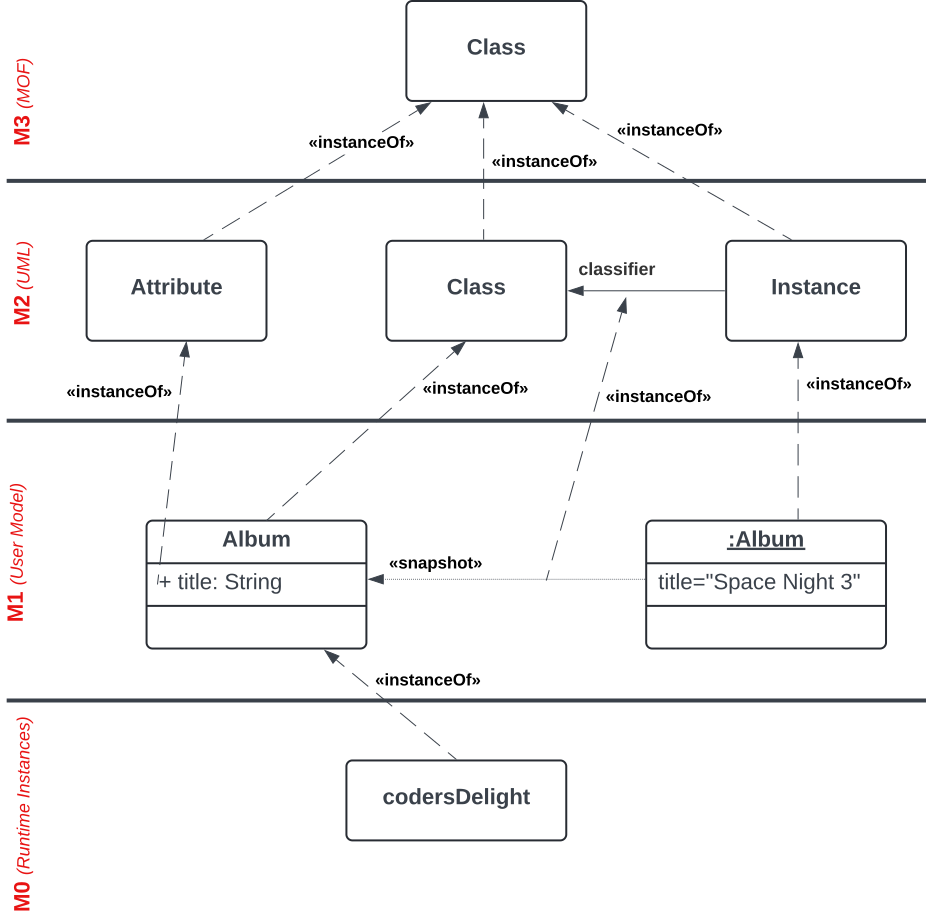
\includegraphics[scale=0.4]{part three/Einführung/img/metamodel}
    \caption{Beispiel für die verschiedenen Schichten der Metamodell Hierarchie.
        In der original Abbildung sind die Pfeilspitzen offen. (Quelle: in Anlehnung an S. 20, Figure 7.8, \url{https://www.omg.org/spec/UML/2.4.1/Infrastructure/PDF}, abgerufen 01.05.2024}
    \label{fig:metamodel-cc}
\end{figure}

\clearpage


\section{Strukturdiagramme}

\begin{tcolorbox}[title=Strukturdiagramme]
    In den \textbf{Strukturdiagrammen} werden \textbf{statische Strukturaspekte} eines Systems betrachtet.
    Für eine Systemmodellierung können alle dieser 6 Diagramme verwendet werden.

    \begin{itemize}
        \item \textbf{Klassendiagramm}: Das \textbf{Klassendiagramm} wird verwendet, um ein objektorientiertes System zu beschreiben.
        \item \textbf{Paketdiagramm}: Ein \textbf{Paketdiagramm} zeigt die Pakete eines Systems und deren Beziehungen.
        \item \textbf{Komponentendiagramm}: Stellt Komponenten oder auch \textit{Subsysteme} mit definierten Interfaces dar, um bspw. \textbf{Architekturdesign} darzustellen.
        \item \textbf{Verteilungsdiagramm}: Beschreibt eine Menge von Knoten, die die \textit{Ausführungsarchitektur} eines Systems definieren können, wobei Knoten i.d.R. \textit{Geräte} oder \textit{Softwareablaufumgebungen repräsentieren}.
        \item \textbf{Kompositionsstrukturdiagramm}: Stellt die \textbf{Komposition} von \textit{Systemstrukturen} (Klassen, Komponenten, Gesamtsystem) in einem bestimmten \textit{Kontext} mit einem bestimmten \textit{Ziel} dar (vgl. \cite[9]{Buh09}).
        \item \textbf{Objektdiagramm}: Momentaufnahme eines Systems zu genau einem \textit{Zeitpukt} während der Ausführung
    \end{itemize}

\end{tcolorbox}
\clearpage

\section{Verhaltensdiagramme}

\begin{tcolorbox}[title=Verhaltensdiagramme]
    \textbf{Verhaltensdiagramme} stellen \textit{Dynamik}, \textit{interne Abläufe} und das \textit{Zusammenspiel} der Systemteile dar, um eine Spezifikation zu vervollständigen.

    \begin{itemize}
        \item \textbf{Anwendungsfalldiagramm}: Dienen zur \textit{Spezifizierung} und \textit{Formalisierung} von \textit{Systemanforderungen}, unter Berücksichtigung von \textbf{Akteuren}, \textbf{Systemen} und \textbf{Anwendungsfällen}
        \item \textbf{Zustandsdiagramm}: Auch \textbf{Zustandsautomaten}; zeigen für ein einzelnes Objekt Zustandsänderungen während der Lebenszeit
        \item \textbf{Aktivitätsdiagramme}: Werden zur Modellierung von \textit{Kontroll}- oder \textit{Objektflüssen} oder zur Darstellung von \textit{Programmlogik} genutzt.
        \item \textbf{Interaktionsdiagramme}: Stellen das Zusammenspiel mehrerer Kommunikationspartner dar.
        Es gibt unterschiedliche Typen von Interaktionsdiagrammen, die Interaktionen auf verschiedenen \textit{Abstraktionsebenen} modellieren:
        \begin{itemize}
            \item \textbf{Sequenzdiagramm}: Zeigt den Verlauf einer Interaktion in zwei Dimensionen, \textit{Kommunikationspartner} und die Nachrichten in ihrer \textit{zeitlichen Abfolge}
            \item \textbf{Kommunikationsdiagramm}: hebt die Kommunikationsbeziehungen zwischen den Partnern hervor
            \item \textbf{Timing Diagramm}: hebt die zeitlichen Aspekte einer Interaktion hervor
            \item \textbf{Interaktionsüberblickdiagramm}: Spezialfall des \textbf{Aktivitätsdiagramms} - statt Aktionen und Aktivitäten können das \textbf{Sequenz}-, \textbf{Kommunikations}- und das \textbf{Timing}-Diagramm als Knoten verwendet werden.
        \end{itemize}
        Alle verwenden dieselben Grundelemente: \textit{Lebenslinien} der Akteure und Nachrichten, die zwischen diesen ausgetauscht werden.
    \end{itemize}
\end{tcolorbox}

\clearpage


\section{Klassendiagramm}

\begin{tcolorbox}[title=Klassendiagramm]
    Das \textbf{Klassendiagramm} beschreibt die Klassen eines Systems und die statischen Beziehungen zwischen ihnen.\\
    Sie werden in Form von Domainklassen bei der \textbf{Analyse} und als detaillierte Entwürfe von Systemklassen als \textit{Blueprint} im \textbf{gesamten Entwicklungsprozess} eingesetzt.

\end{tcolorbox}
\clearpage


\section{Assoziationsklasse (Attributierte Assoziation)}

\begin{tcolorbox}[title=Assoziationsklasse (Attributierte Assoziation)]
Eine \textbf{Assoziationsklasse} erlaubt das Hinzufügen von Operationen und Attributen zu einer Assoziation (\cite[43]{Buh09}).\\
Assoziationsklassen werden in der \textbf{Analyse} in Modellen verwendet und in dem \textbf{Entwurf} in eigenständige Klassen transformiert.\\

\noindent
Assoziationsklassen werden in der \textbf{Analyse} in Modellen verwendet und in dem \textbf{Entwurf} in eigenständige Klassen transformiert.

\blockquote[{\cite[277]{Oes05}}]{
    Eine attributierte Assoziation ist immer dann nahe liegend, wenn Attribute oder Operationen gefunden werden, die weder der einen noch der anderen Klasse zugeordnet werden können, weil sie nämlich Eigenschaften der Beziehung selbst sind.
}.\\

Bei einer attributierten Assoziation dürfen zwei beteiligte Objekte maximal nur eine Beziehung zueinander haben (vgl.~\cite[277]{Oes05})\footnote{
    \textit{Ostereich} führt dies ebenda auf Seite 278 weiter aus, in dem er beschreibt, wie eine attributierte Assoziation für ein \textit{Beschäftigtenverhältnis} zwischen \textit{Mitarbeiter} und \textit{Unternehmen} modelliert wird. Dabei wird davon ausgegangen, dass ein \textit{Mitarbeiter} nur über \textit{ein} Arbeitsverhältnis mit einem \textit{Unternehmen} in Beziehung stehen kann. Bestehen mehrere Arbeitsverhältnisse (\textit{Mitarbeiter} hat zu unterschiedlichen Zeitpunkten für das \textit{Unternehmen} gearbeitet), kann die attributierte Assoziation nicht verwendet werden.\\

\noindent
Wird eine attributierte Assoziation in eine gewöhnliche Assoziation transformiert, muss darauf geachtet werden, die Multiplizitäten richtig zu setzen (s. Abbildung~\ref{fig:assoziationsklasse}).
\end{tcolorbox}

\begin{figure}
    \centering
    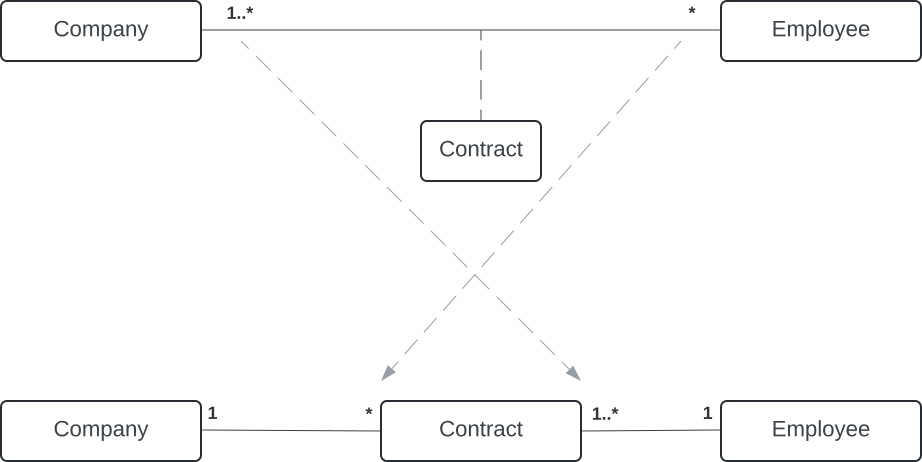
\includegraphics[scale=0.4]{part three/Klassendiagramme - Erweiterte Konzepte und Paketdiagramme/img/assoziationsklasse}
    \caption{Darstellung einer Assoziation mit Hilfe einer Assoziationsklasse (oben) sowie Transformation in gewöhnliche Assoziationen (unten). (Quelle: in Anlehnung an \cite[279, Abb. 4.4-11]{Oes05})}
    \label{fig:assoziationsklasse-cc}
\end{figure}

\clearpage


\section{Sequenzdiagramme}

\begin{tcolorbox}[title=Sequenzdiagramme]
    \textbf{Sequenzdiagramme} stellen Verhalten auf der Ebene einer Interaktion dar.\\
    In der Phase des Klassendesigns werden die Teilnehmer der Interaktionen bestimmt, weshalb Sequenzdiagramme oft in dieser Phase genutzt werden.\\
    In der \textbf{Analysephase} können Sequenzdiagramme eingesetzt werden, um die Kommunikation der bis dahin ausgemachten \textbf{Geschäftsobjekte} zu modellieren, oder um \textbf{Anwendungsfälle} weiter zu spezifizieren.
\end{tcolorbox}
\clearpage

\section{Aggregation}

\begin{tcolorbox}[title=Aggregation]
    Eine \textbf{Aggregation} ist in ihrer \semantischen Aussage unscharf (vgl.~\cite[40]{Buh09}).\\
    Sie beschreibt eine \textit{Ganzes}-\textit{Teile}-Beziehung, aber die \textit{Teile} können zu mehreren verschiedenen \textit{Ganzen} gehören.\\
    Außerdem kann ein Teil dem \textit{Ganzen} jederzeit wieder entnommen werden und das \textit{Ganze} ist nicht verantwortlich für das Erstellen der \textit{Teile}, weshalb Implementierungen beim Hinzufügen von Teilen oft schon fertige Objekte erwarten, die jeweils eines der \textit{Teile} repräsentieren.\\
    Aggregationsbeziehungen werden durch eine nicht-gefüllte Raute an der Seite der Klasse, die das Ganze repräsentiert, dargestellt.
\end{tcolorbox}
\clearpage

\section{Komposition}

\begin{tcolorbox}[title=Komposition]
    Bei einer \textbf{Komposition} handelt es sich um eine \textit{Ganzes}-\textit{Teile}-Beziehung, bei der das \textit{Ganze} verantwortlich für die Erstellung und Beseitigung der \textit{Teile} ist.
    Außerdem sind die \textit{Teile} an die \textbf{Existenz} des \textit{Ganzen} gebunden.\\
    \textit{Teile} gehören immer zu \textit{genau einem} \textit{Ganzen}.\\
    Eine Komposition wird dargestellt durch eine gefüllte Raute an der Klassenbox, die das \textit{Ganze} repräsentiert.
\end{tcolorbox}
\clearpage

\section{Paketdiagramm}

\begin{tcolorbox}[title=Komposition]
    \textbf{Paketdiagramme} zeigen Pakete und ihre Abhängigkeiten und werden in frühen Designphasen genutzt, um Strukturen (großer Systeme) aufzuzeigen.\\

    \noindent
    Elemente sollten so in Paketen gruppiert werden, dass ihr \textbf{funktionaler Zusammenhalt} (\textit{Kohäsion}, s. Abschnitt~\ref{subsec:hohe-kohasion}) klar wird.\\
    Hierdurch kann vermieden werden, dass Änderungen einer Klasse eines Paketes auch Änderungen außerhalb des Paketes erfordern.\\
    Außerdem erhöht sich die Wahrscheinlichkeit, dass einzelne Pakete als solche in anderen Projekten wiederverwendet werden können.\\

    \noindent
    In Paketdiagrammen können Beziehungen über folgende Schlüsselwörter deutlich gemacht werden:

    \begin{itemize}
        \item \guillemotleft import\guillemotright
        \item[] $\rightarrow$ \textbf{public-Import} zwischen Quell- und Zielpaket; Quellpaket kann die öffentlichen Elemente des Zielpaketes unter Verwendung des unqualifizierten und des qualifizierten Namens verwenden; die importierten Elemente sind auch für Pakete sichtbar, die das Quellpaket importieren
        \item \guillemotleft access\guillemotright
        \item[] $\rightarrow$ \textbf{privater Import} zwischen Quell- und Zielpaket; Zugriff auf Elemente des importierten Paketes ohne qualifizierenden Namen möglich; der Import eines Paketes in \textbf{Java} entspricht der \guillemotleft access\guillemotright-Beziehung
        \item \guillemotleft merge\guillemotright
        \item[] $\rightarrow$ Bei einem \textbf{merge} werden Elemente eines Zielpaketes in das Quellpaket
   \end{itemize}
\end{tcolorbox}
\clearpage

\section{Anwendungsfalldiagramm}

\begin{tcolorbox}[title=Anwendungsfalldiagramm]
    Die \textbf{Anwendungsfallanalyse} wird im Rahmen der \textbf{Anforderungsspezifikation} eingesetzt.\\

    \noindent
    Anwendungsfalldiagramme sind das am häufigsten eingesetzte Mittel zur Aufnahme und Darstellung von \textbf{Anforderungen}.\\
    Sie beschreiben selbst kein Verhalten und keine Abläufe, sondern zeigen nur die Zusammenhänge der an Anwendungsfällen beteiligten Modellelemente und sind somit ein Hilfsmittel zur Anforderungsermittlung und Verwaltung.\\

    \noindent
    Zu den wichtigsten Schritten einer Anwendungsfallanalyse gehören:
    \begin{enumerate}
        \item Akteure identifizieren
        \item Anwendungsfälle identifizieren
        \item Beschreiben der Akteure und Anwendungsfälle
        \item Identifizieren von \textit{Schlüsselobjekten}, die das System verwaltet
        \item Identifizieren der wichtigsten Anwendungsfälle (Priorisierung)
        \item detailliertere Beschreibung der Anwendungsfälle
        \item Strukturierung des Anwendungsfalldiagramms
    \end{enumerate}

    \noindent
    Anwendungsfälle beschreiben das \textbf{Szenario} der Nutzung, und nicht Features des Systems.
\end{tcolorbox}

\clearpage

\input{chapters/Anhang/CheatSheets/SE3/Aktivitätsdiagramm}
\clearpage

\section{Zustandsautomat}

\begin{tcolorbox}[title=Zustandsautomat]
    Mit \textbf{Zustandsautomaten} kann das \textit{Verhalten} von Systemen modelliert werden, wobei die \textit{Reaktionen} des Systems im Mittelpunkt stehen, und nicht die \textit{Aktionen}, wie bspw. bei den \textbf{Aktivitätsdiagrammen}.\\

    \noindent
        Ein \textbf{Zustandsautomat} kann den \textit{Lebensweg} eines Objektes modellieren, weshalb Zustandsautomaten oft im \textbf{Entwurf} als Ergänzung zu den \textbf{Klassendiagrammen} eingesetzt werden.
\end{tcolorbox}

\begin{figure}
    \centering
    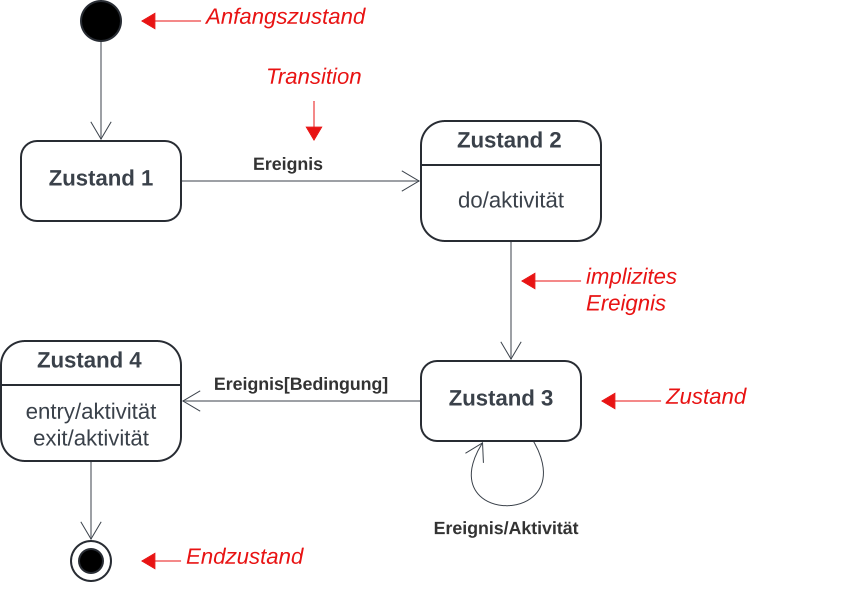
\includegraphics[scale=0.4]{part three/Zustandsautomaten/img/statechartdiagramnotation}
    \caption{Elemente eines einfachen Zustandsautomaten. Eine Transitionen wird durch ein \textbf{Ereignis} ausgelöst, das ein \textit{Signal}, ein \textit{Operationsaufruf} oder auch eine bestimmte \textit{Attributänderung} sein kann. (Quelle: in Anlehnung an \cite[90, Abb. 2.11-6]{Bal05})}
    \label{fig:statechartdiagramnotation-cc}
\end{figure}

\begin{minted}[fontsize=\small]{java}
// Beispiel für eine Implementierung eines
// Parkscheinautomaten als Zustandsautomat in Java
class Parkscheinautomat {

  // zustände
  private final int BEREIT = 0;
  private final int ZAHLUNG = 1;
  private final int ABBRUCH = 2;
  private final int BELEG   = 3;

  // Zustand; wird initial beim Starten
  // des Automaten gesetzt
  private int zustand;

  // Methoden lösen Aktionen beim Eintritt
  // in die jeweiligen Zustände aus
  private int zahlung() {
    // verarbeiten
    // danach neuen Zustand zurückliefern...
    ...
    return BEREIT;
  }

   ...

  private void bereit() {
    while (true) {
      // eingabe überprüfen und
      // ggf. Zustandswechsel auslösen:
      // Zustand als Attribut setzen
      ...
    }
  }

  public void start() {
    zustand = BEREIT;

    while(true) {
      switch (zustand) {
        case BEREIT:
          zustand = bereit();
        // ... weiteres Verhalten
        ...
      }
    }
  }
}
\end{minted}
\clearpage
	

\section{Inhalt SE3}

\section*{1. Übersicht UML}

\subsection*{Lernziele}
\begin{itemize}
    \item einen Einblick in den Sprachaufbau der UML 2.0 gewinnen
    \item einen Überblick über die Diagramme der UML 2.0 und deren Zweck haben
\end{itemize}

\subsection*{Zusammenfassung}
\begin{itemize}
    \item Die \textbf{UML} ist eine weit verbreitete Modellierungssprache zur Modellierung objektorientierter Softwaresysteme.
    \item Die UML 2.0 Spezifikation besteht aus vier Teilen:
    \begin{enumerate}
        \item \textbf{Superstructure}: Diagrammtypen
        \item \textbf{Infrastructure}: Modellierungskonzepte
        \item \textbf{OCL}: formale Sprache zur Formulierung von Einschränkungen
        \item \textbf{Diagram Interchange}: Austauschformate
    \end{enumerate}
    \item Die UML kann im \textbf{Sketching} oder \textbf{Blueprint Modus} eingesetzt werden, oder als Grundlage für \textbf{automatische Codegenerierung}
    \item Die UML ist an keinen speziellen Entwicklungsprozess gebunden
\end{itemize}

\section*{2. Klassendiagramme}

\subsection*{Lernziele}
\begin{itemize}
    \item wissen, wie Klassendiagramme im Entwicklungsprozess eingesetzt werden
    \item Klassendiagramme für Analyse- und Designentscheidungen einsetzen können
    \item die wichtigsten Modellierungskonzepte kennen
    \item sinnvolle Klassendiagramme erstellen und Java-Implementierungen ableiten können
    \item Klassendiagramme aus Java Quellcode erzeugen können
\end{itemize}

\subsection*{Zusammenfassung}

\begin{itemize}
    \item \textbf{Klassendiagramme} dienen zur \textbf{strukturellen Darstellung} von Softwaresystemen
    \item hierbei werden Klassen und \textbf{Beziehungen} zwischen Klassen dargestellt
    \item Properties können durch die \textbf{Attribut}- oder \textbf{Assoziationsnotation} modelliert werden
    \item Operationen werden als separate Zeile in ihrem Compartment dargestellt
    \item im Klassendiagramm können auch \textbf{Generalisierungsbeziehungen} modelliert werden
    \item \textbf{Abhängigkeitsbeziehungen} drücken ein Verhältnis zwischen \textbf{Client} und \textbf{Supplier} aus
\end{itemize}

\section*{3. Objektorientierter Entwurf}

\subsection*{Lernziele}
\begin{itemize}
    \item das Wesen einer Interaktion kennen
    \item wissen, wie Sequenzdiagramme im Entwicklungsprozess eingesetzt werden
    \item Sequenzdiagramme für Analyse- und Designentscheidungen sowie zur Darstellung von Kontrollflüssen einsetzen können
    \item die wichtigsten Modellierungskonzepte kennen
    \item sinnvolle Sequenzdiagramme erstellen und Java-Implementierungen ableiten können
    \item Sequenzdiagramme aus Java Quellcode erzeugen können
\end{itemize}

\subsection*{Zusammenfassung}

\begin{itemize}
    \item Sequenzdiagramme sind \textbf{Verhaltensdiagramme}
    und können im gesamten Entwicklungszyklus zur Modellierung von Interaktionen angewendet werden
    \item Interaktionen bestehen im Wesentlichen aus dem Nachrichtenaustausch zwischen verschiedenen Kommunikationspartnern
    \item in den meisten Fällen wird die Kommunikation von Objekten von Klassen modelliert, aber es können auch Teilnehmer auf anderen Ebenen modelliert werden
    \item gewöhnlich gibt ein Sequenzdiagramm einen \textbf{Anwendungsfall} (\textit{Szenario}) wieder
    \item sie dienen nicht dazu, um Zustandsänderungen darzustellen (hierfür werden Zustandsdiagramme verwendet)
    \item Sequenzdiagramme sind \textit{nicht} gut geeignet für die Darstellung von
    \begin{itemize}
        \item nebenläufigem Verhalten (\textit{asynchrone} Nachrichten, \textit{kombiniertes Fragment})
        \item Schleifen und alternativem Verhalten (\textit{kombinierte Fragmente})
        \item[] $\rightarrow$  für beide Fälle sind \textbf{Aktivitätsdiagramme} besser geeignet
    \end{itemize}
\end{itemize}

\section*{4. Klassendiagramme - Erweiterte Konzepte und Paketdiagramme}

\subsection*{Lernziele}
\begin{itemize}
    \item erweiterte Modellierungskonzepte in Klassendiagrammen für den Detailentwurf von Systemen kennen
    \item die Konsequenzen dieser Konzepte in der Implementierung kennen
    \item wissen, wie Paketdiagramme im Entwicklungsprozess eingesetzt werden
    \item die Modellierungskonzepte in Paketdiagrammen kennen
    \item anhand von Paketdiagrammen Software-Architekturen gestalten und bewerten können
\end{itemize}

\subsection*{Zusammenfassung}

\begin{itemize}
    \item Die vorgestellten erweiterten Konzepte werden vor allem im \textbf{Feinentwurf} von Klassenstrukturen eingesetzt.
    \item Generell gilt, dass die Spezifikationen von Objekten und Properties nur so detailliert ausgeführt werden sollen, wie nötig: Sind Details für das Verständnis unnötig, sollte darauf verzichtet werden.
    \item \textbf{Generalisierungsbeziehungen} sollten grundsätzlich modelliert werden.
    \item Ist eine \textbf{Komposition} statt einer Generalisierung für den Sachverhalt möglich, sollte diese verwendet werden: ``Favor object composition over inheritance.`` (\cite[19 f.]{GHJV94})
    \item \textbf{Kompositionsbeziehungen} geben eindeutige Impulse für eine Implementierung, \textbf{Aggregationsbeziehungen} sind in ihrer semantischen Aussage nicht sehr eindeutig
    \item \textbf{Assoziationsklassen} sind in ihrer frühen Designphase empfehlenswert, die Realisierung (mit {bspw.} Java) erfordert aber eine Transformation in eine volle Klasse, wobei die Multiplizitäten angepasst werden müssen
    \item Elemente können in \textbf{Paketen} zusamengefasst und unter einem gemeinsamen Namensraum gruppiert werden
\end{itemize}

\section*{4. Anwendungsfalldiagramm (Use-Case-Diagramm)}

\subsection*{Lernziele}
\begin{itemize}
    \item wissen, wie die Anwendungsfallanalyse im Rahmen der Anforderungsspezifikation eingesetzt wird
    \item Prozessschritte der Anwendungsfallanalyse beherrschen
    \item die wichtigsten Modellierungskonzepte in Anwendungsfalldiagrammen kennen
    \item den Aufbau einer Anwendungsfallbeschreibung kennen
\end{itemize}

\subsection*{Zusammenfassung}

\begin{itemize}
    \item \textbf{Anwendungsfalldiagramme} besitzen eine einfache Notation, um \textbf{Akteure} und \textbf{Anwendungsfälle} eines \textbf{Systems} grafisch darzustellen
    \item auf Basis eines Anwendungsfalldiagramms lässt sich ermitteln, ob die Anwendungsfälle gewünschtes Verhalten realisieren bzw. Beziehungen zu einem oder mehreren Akteuren haben
    \item Anwendungsfälle und Akteure \textit{müssen} zusätzlich textlich beschrieben werden
\end{itemize}

\section*{5. Aktivitätsdiagramme}

\subsection*{Lernziele}
\begin{itemize}
    \item wissen, wie Aktivitätsdiagramme im Rahmen der Verhaltensanalyse in verschiedenen Prozessphasen eingesetzt werden können
    \item die wichtigsten Modellierungskonzepte in Aktivitätsdiagrammen kennen
    \item Aktivitätsdiagramme interpretieren, erstellen und implementieren können
\end{itemize}

\subsection*{Zusammenfassung}

\begin{itemize}
    \item \textbf{Aktivitätsdiagramme} gehören zu den \textbf{Verhaltensdiagrammen} und können im \textit{gesamten} \textbf{Entwicklungsprozess} eingesetzt werden
    \item durch ein Aktivitätsdiagramm kann gezeigt werden, wie \textbf{Verhalten} realisiert wird
    \item es können mehrere \textbf{Aktivitäten} dargestellt werden
    \item \textbf{Aktivitätskanten} und \textbf{Aktivitätsknoten} werden zur Beschreibung von Verhalten verwendet
\end{itemize}

\section*{5. Zustandsautomaten}

\subsection*{Lernziele}
\begin{itemize}
    \item wissen, wie Zustandsdiagramme im Rahmen der Verhaltensanalyse einzelner Objekte eingesetzt werden können
    \item die wichtigsten Modellierungskonzepte in Zustandsdiagrammen kennen
    \item Zustandsdiagramme interpretieren, erstellen und implementieren können
\end{itemize}

\subsection*{Zusammenfassung}

\begin{itemize}
    \item Das \textbf{Zustandsdiagramm} gehört wie das \textbf{Aktivitätsdiagramm} zu den \textbf{Verhaltensdiagrammen}.
    \item Ein Zustandsdiagramm zeigt den \textbf{Lebensweg} eines \textbf{Objektes}.
    \item \textbf{Attributwerte} bestimmen den Zustand eines Objektes.
    \item \textbf{Transitionen} zwischen Zuständen werden durch \textbf{Guards} und \textbf{Events} gesteuert.
    \item Während der Transitionen können \textbf{Effekte} (\textit{Aktivitäten}) realisiert werden.
    \item Die Modellierung \textbf{zusammengesetzter Zustände} ist ebenfalls möglich.
    \item Für die Darstellung \textbf{paralleler} oder  \textbf{konkurrierender} Abläufe können \textbf{Regionen} modelliert werden.
\end{itemize}
\clearpage


\section{UML Modellierung}

\begin{tcolorbox}[title=UML Modellierung]
    \textbf{Modelle} haben die Aufgabe, den Bezug zum Original (Programm, Softwaresystem) herzustellen, sowie zu der \textit{Anwendungsumgebung}.\\
    Ein \textbf{Modell} enthält alle \textbf{Modellelemente}, die zur Beschreibung eines Softwaresystems nötig sind.\\

    \noindent
    Ein \textbf{Modellelement} wird als Element in einem UML Modell von einem Benutzer erstellt und auf verschiedenen \textbf{Diagrammen} (Struktur-/Verhaltensdiagrammen) platziert, und wird durch die \textbf{UML Modellierungskonzepte} als Metaklasse des \textbf{Metamodells} der UML beschrieben: \textbf{Modellelemente} werden aus Modellierungskonzepten instanziiert.\\

    \noindent
       Das \textbf{UML Metamodell} regelt, in welchem Zusammenhang \textbf{UML Modellierungskonzepte} in Modellen auftreten dürfen, und welche Eigenschaften und Beziehungen zu anderen Sprachelementen zulässig sind.\\

       \noindent
       Die im \textbf{Metamodell} verwendeten Erklärungen basieren auf einer abstrakten Syntax, für deren Beschreibung eine Untermenge (\textit{Klassendiagramme}) der UML verwendet wird.\\
        Die \textbf{Semantik} der Modellierungskonzepte wird textlich beschrieben, zur Formalisierung von Regeln für die syntaktische Korrektheit wird die \textbf{OCL} (\textit{Object Constraint Language}) verwendet.
\end{tcolorbox}

\begin{figure}
    \centering
    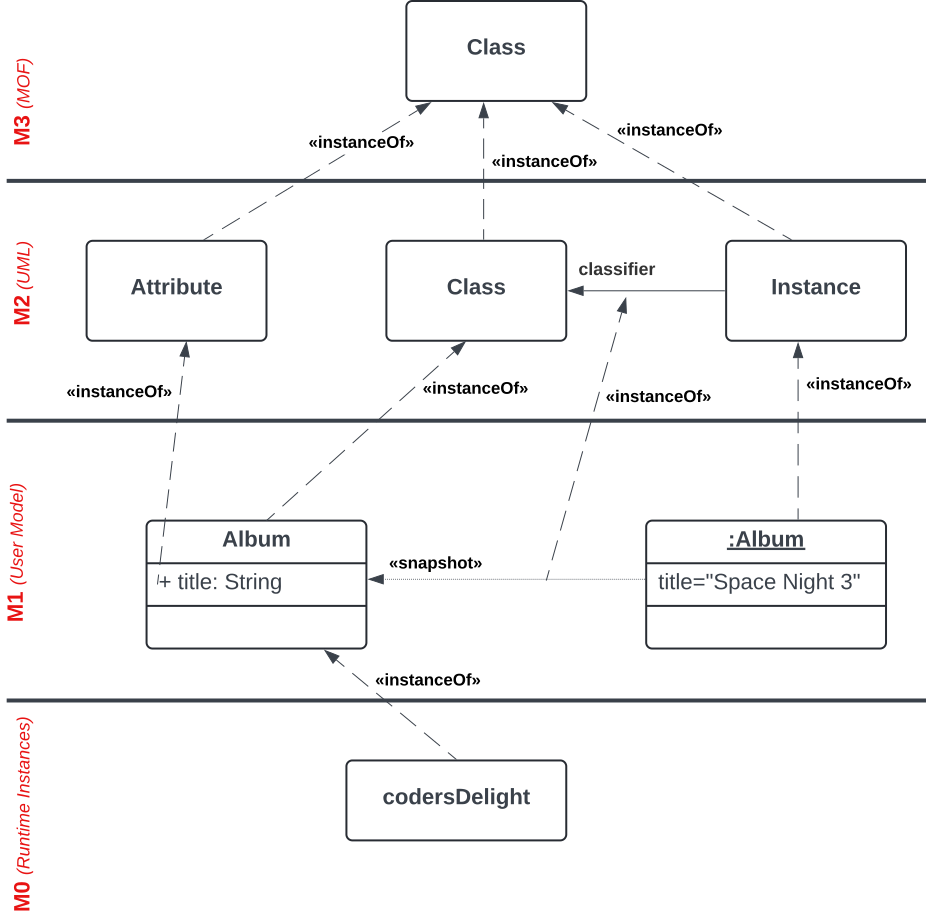
\includegraphics[scale=0.4]{part three/Einführung/img/metamodel}
    \caption{Beispiel für die verschiedenen Schichten der Metamodell Hierarchie.
        In der original Abbildung sind die Pfeilspitzen offen. (Quelle: in Anlehnung an S. 20, Figure 7.8, \url{https://www.omg.org/spec/UML/2.4.1/Infrastructure/PDF}, abgerufen 01.05.2024}
    \label{fig:metamodel-cc}
\end{figure}

\clearpage


\section{Strukturdiagramme}

\begin{tcolorbox}[title=Strukturdiagramme]
    In den \textbf{Strukturdiagrammen} werden \textbf{statische Strukturaspekte} eines Systems betrachtet.
    Für eine Systemmodellierung können alle dieser 6 Diagramme verwendet werden.

    \begin{itemize}
        \item \textbf{Klassendiagramm}: Das \textbf{Klassendiagramm} wird verwendet, um ein objektorientiertes System zu beschreiben.
        \item \textbf{Paketdiagramm}: Ein \textbf{Paketdiagramm} zeigt die Pakete eines Systems und deren Beziehungen.
        \item \textbf{Komponentendiagramm}: Stellt Komponenten oder auch \textit{Subsysteme} mit definierten Interfaces dar, um bspw. \textbf{Architekturdesign} darzustellen.
        \item \textbf{Verteilungsdiagramm}: Beschreibt eine Menge von Knoten, die die \textit{Ausführungsarchitektur} eines Systems definieren können, wobei Knoten i.d.R. \textit{Geräte} oder \textit{Softwareablaufumgebungen repräsentieren}.
        \item \textbf{Kompositionsstrukturdiagramm}: Stellt die \textbf{Komposition} von \textit{Systemstrukturen} (Klassen, Komponenten, Gesamtsystem) in einem bestimmten \textit{Kontext} mit einem bestimmten \textit{Ziel} dar (vgl. \cite[9]{Buh09}).
        \item \textbf{Objektdiagramm}: Momentaufnahme eines Systems zu genau einem \textit{Zeitpukt} während der Ausführung
    \end{itemize}

\end{tcolorbox}
\clearpage

\section{Verhaltensdiagramme}

\begin{tcolorbox}[title=Verhaltensdiagramme]
    \textbf{Verhaltensdiagramme} stellen \textit{Dynamik}, \textit{interne Abläufe} und das \textit{Zusammenspiel} der Systemteile dar, um eine Spezifikation zu vervollständigen.

    \begin{itemize}
        \item \textbf{Anwendungsfalldiagramm}: Dienen zur \textit{Spezifizierung} und \textit{Formalisierung} von \textit{Systemanforderungen}, unter Berücksichtigung von \textbf{Akteuren}, \textbf{Systemen} und \textbf{Anwendungsfällen}
        \item \textbf{Zustandsdiagramm}: Auch \textbf{Zustandsautomaten}; zeigen für ein einzelnes Objekt Zustandsänderungen während der Lebenszeit
        \item \textbf{Aktivitätsdiagramme}: Werden zur Modellierung von \textit{Kontroll}- oder \textit{Objektflüssen} oder zur Darstellung von \textit{Programmlogik} genutzt.
        \item \textbf{Interaktionsdiagramme}: Stellen das Zusammenspiel mehrerer Kommunikationspartner dar.
        Es gibt unterschiedliche Typen von Interaktionsdiagrammen, die Interaktionen auf verschiedenen \textit{Abstraktionsebenen} modellieren:
        \begin{itemize}
            \item \textbf{Sequenzdiagramm}: Zeigt den Verlauf einer Interaktion in zwei Dimensionen, \textit{Kommunikationspartner} und die Nachrichten in ihrer \textit{zeitlichen Abfolge}
            \item \textbf{Kommunikationsdiagramm}: hebt die Kommunikationsbeziehungen zwischen den Partnern hervor
            \item \textbf{Timing Diagramm}: hebt die zeitlichen Aspekte einer Interaktion hervor
            \item \textbf{Interaktionsüberblickdiagramm}: Spezialfall des \textbf{Aktivitätsdiagramms} - statt Aktionen und Aktivitäten können das \textbf{Sequenz}-, \textbf{Kommunikations}- und das \textbf{Timing}-Diagramm als Knoten verwendet werden.
        \end{itemize}
        Alle verwenden dieselben Grundelemente: \textit{Lebenslinien} der Akteure und Nachrichten, die zwischen diesen ausgetauscht werden.
    \end{itemize}
\end{tcolorbox}

\clearpage


\section{Klassendiagramm}

\begin{tcolorbox}[title=Klassendiagramm]
    Das \textbf{Klassendiagramm} beschreibt die Klassen eines Systems und die statischen Beziehungen zwischen ihnen.\\
    Sie werden in Form von Domainklassen bei der \textbf{Analyse} und als detaillierte Entwürfe von Systemklassen als \textit{Blueprint} im \textbf{gesamten Entwicklungsprozess} eingesetzt.

\end{tcolorbox}
\clearpage


\section{Assoziationsklasse (Attributierte Assoziation)}

\begin{tcolorbox}[title=Assoziationsklasse (Attributierte Assoziation)]
Eine \textbf{Assoziationsklasse} erlaubt das Hinzufügen von Operationen und Attributen zu einer Assoziation (\cite[43]{Buh09}).\\
Assoziationsklassen werden in der \textbf{Analyse} in Modellen verwendet und in dem \textbf{Entwurf} in eigenständige Klassen transformiert.\\

\noindent
Assoziationsklassen werden in der \textbf{Analyse} in Modellen verwendet und in dem \textbf{Entwurf} in eigenständige Klassen transformiert.

\blockquote[{\cite[277]{Oes05}}]{
    Eine attributierte Assoziation ist immer dann nahe liegend, wenn Attribute oder Operationen gefunden werden, die weder der einen noch der anderen Klasse zugeordnet werden können, weil sie nämlich Eigenschaften der Beziehung selbst sind.
}.\\

Bei einer attributierten Assoziation dürfen zwei beteiligte Objekte maximal nur eine Beziehung zueinander haben (vgl.~\cite[277]{Oes05})\footnote{
    \textit{Ostereich} führt dies ebenda auf Seite 278 weiter aus, in dem er beschreibt, wie eine attributierte Assoziation für ein \textit{Beschäftigtenverhältnis} zwischen \textit{Mitarbeiter} und \textit{Unternehmen} modelliert wird. Dabei wird davon ausgegangen, dass ein \textit{Mitarbeiter} nur über \textit{ein} Arbeitsverhältnis mit einem \textit{Unternehmen} in Beziehung stehen kann. Bestehen mehrere Arbeitsverhältnisse (\textit{Mitarbeiter} hat zu unterschiedlichen Zeitpunkten für das \textit{Unternehmen} gearbeitet), kann die attributierte Assoziation nicht verwendet werden.\\

\noindent
Wird eine attributierte Assoziation in eine gewöhnliche Assoziation transformiert, muss darauf geachtet werden, die Multiplizitäten richtig zu setzen (s. Abbildung~\ref{fig:assoziationsklasse}).
\end{tcolorbox}

\begin{figure}
    \centering
    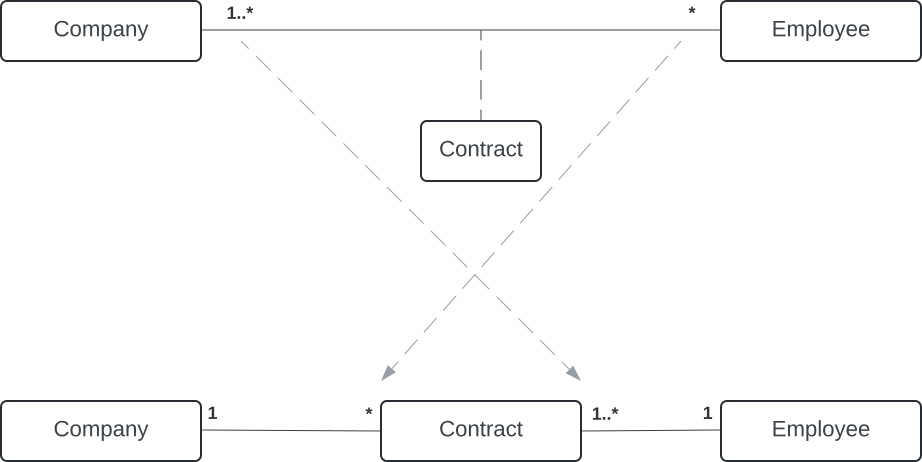
\includegraphics[scale=0.4]{part three/Klassendiagramme - Erweiterte Konzepte und Paketdiagramme/img/assoziationsklasse}
    \caption{Darstellung einer Assoziation mit Hilfe einer Assoziationsklasse (oben) sowie Transformation in gewöhnliche Assoziationen (unten). (Quelle: in Anlehnung an \cite[279, Abb. 4.4-11]{Oes05})}
    \label{fig:assoziationsklasse-cc}
\end{figure}

\clearpage


\section{Sequenzdiagramme}

\begin{tcolorbox}[title=Sequenzdiagramme]
    \textbf{Sequenzdiagramme} stellen Verhalten auf der Ebene einer Interaktion dar.\\
    In der Phase des Klassendesigns werden die Teilnehmer der Interaktionen bestimmt, weshalb Sequenzdiagramme oft in dieser Phase genutzt werden.\\
    In der \textbf{Analysephase} können Sequenzdiagramme eingesetzt werden, um die Kommunikation der bis dahin ausgemachten \textbf{Geschäftsobjekte} zu modellieren, oder um \textbf{Anwendungsfälle} weiter zu spezifizieren.
\end{tcolorbox}
\clearpage

\section{Aggregation}

\begin{tcolorbox}[title=Aggregation]
    Eine \textbf{Aggregation} ist in ihrer \semantischen Aussage unscharf (vgl.~\cite[40]{Buh09}).\\
    Sie beschreibt eine \textit{Ganzes}-\textit{Teile}-Beziehung, aber die \textit{Teile} können zu mehreren verschiedenen \textit{Ganzen} gehören.\\
    Außerdem kann ein Teil dem \textit{Ganzen} jederzeit wieder entnommen werden und das \textit{Ganze} ist nicht verantwortlich für das Erstellen der \textit{Teile}, weshalb Implementierungen beim Hinzufügen von Teilen oft schon fertige Objekte erwarten, die jeweils eines der \textit{Teile} repräsentieren.\\
    Aggregationsbeziehungen werden durch eine nicht-gefüllte Raute an der Seite der Klasse, die das Ganze repräsentiert, dargestellt.
\end{tcolorbox}
\clearpage

\section{Komposition}

\begin{tcolorbox}[title=Komposition]
    Bei einer \textbf{Komposition} handelt es sich um eine \textit{Ganzes}-\textit{Teile}-Beziehung, bei der das \textit{Ganze} verantwortlich für die Erstellung und Beseitigung der \textit{Teile} ist.
    Außerdem sind die \textit{Teile} an die \textbf{Existenz} des \textit{Ganzen} gebunden.\\
    \textit{Teile} gehören immer zu \textit{genau einem} \textit{Ganzen}.\\
    Eine Komposition wird dargestellt durch eine gefüllte Raute an der Klassenbox, die das \textit{Ganze} repräsentiert.
\end{tcolorbox}
\clearpage

\section{Paketdiagramm}

\begin{tcolorbox}[title=Komposition]
    \textbf{Paketdiagramme} zeigen Pakete und ihre Abhängigkeiten und werden in frühen Designphasen genutzt, um Strukturen (großer Systeme) aufzuzeigen.\\

    \noindent
    Elemente sollten so in Paketen gruppiert werden, dass ihr \textbf{funktionaler Zusammenhalt} (\textit{Kohäsion}, s. Abschnitt~\ref{subsec:hohe-kohasion}) klar wird.\\
    Hierdurch kann vermieden werden, dass Änderungen einer Klasse eines Paketes auch Änderungen außerhalb des Paketes erfordern.\\
    Außerdem erhöht sich die Wahrscheinlichkeit, dass einzelne Pakete als solche in anderen Projekten wiederverwendet werden können.\\

    \noindent
    In Paketdiagrammen können Beziehungen über folgende Schlüsselwörter deutlich gemacht werden:

    \begin{itemize}
        \item \guillemotleft import\guillemotright
        \item[] $\rightarrow$ \textbf{public-Import} zwischen Quell- und Zielpaket; Quellpaket kann die öffentlichen Elemente des Zielpaketes unter Verwendung des unqualifizierten und des qualifizierten Namens verwenden; die importierten Elemente sind auch für Pakete sichtbar, die das Quellpaket importieren
        \item \guillemotleft access\guillemotright
        \item[] $\rightarrow$ \textbf{privater Import} zwischen Quell- und Zielpaket; Zugriff auf Elemente des importierten Paketes ohne qualifizierenden Namen möglich; der Import eines Paketes in \textbf{Java} entspricht der \guillemotleft access\guillemotright-Beziehung
        \item \guillemotleft merge\guillemotright
        \item[] $\rightarrow$ Bei einem \textbf{merge} werden Elemente eines Zielpaketes in das Quellpaket
   \end{itemize}
\end{tcolorbox}
\clearpage

\section{Anwendungsfalldiagramm}

\begin{tcolorbox}[title=Anwendungsfalldiagramm]
    Die \textbf{Anwendungsfallanalyse} wird im Rahmen der \textbf{Anforderungsspezifikation} eingesetzt.\\

    \noindent
    Anwendungsfalldiagramme sind das am häufigsten eingesetzte Mittel zur Aufnahme und Darstellung von \textbf{Anforderungen}.\\
    Sie beschreiben selbst kein Verhalten und keine Abläufe, sondern zeigen nur die Zusammenhänge der an Anwendungsfällen beteiligten Modellelemente und sind somit ein Hilfsmittel zur Anforderungsermittlung und Verwaltung.\\

    \noindent
    Zu den wichtigsten Schritten einer Anwendungsfallanalyse gehören:
    \begin{enumerate}
        \item Akteure identifizieren
        \item Anwendungsfälle identifizieren
        \item Beschreiben der Akteure und Anwendungsfälle
        \item Identifizieren von \textit{Schlüsselobjekten}, die das System verwaltet
        \item Identifizieren der wichtigsten Anwendungsfälle (Priorisierung)
        \item detailliertere Beschreibung der Anwendungsfälle
        \item Strukturierung des Anwendungsfalldiagramms
    \end{enumerate}

    \noindent
    Anwendungsfälle beschreiben das \textbf{Szenario} der Nutzung, und nicht Features des Systems.
\end{tcolorbox}

\clearpage

\input{chapters/Anhang/CheatSheets/SE3/Aktivitätsdiagramm}
\clearpage

\section{Zustandsautomat}

\begin{tcolorbox}[title=Zustandsautomat]
    Mit \textbf{Zustandsautomaten} kann das \textit{Verhalten} von Systemen modelliert werden, wobei die \textit{Reaktionen} des Systems im Mittelpunkt stehen, und nicht die \textit{Aktionen}, wie bspw. bei den \textbf{Aktivitätsdiagrammen}.\\

    \noindent
        Ein \textbf{Zustandsautomat} kann den \textit{Lebensweg} eines Objektes modellieren, weshalb Zustandsautomaten oft im \textbf{Entwurf} als Ergänzung zu den \textbf{Klassendiagrammen} eingesetzt werden.
\end{tcolorbox}

\begin{figure}
    \centering
    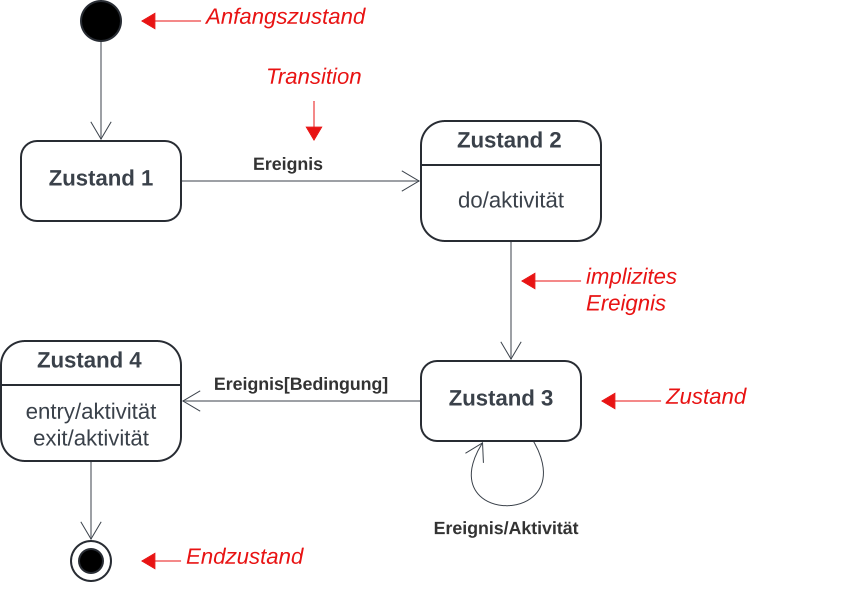
\includegraphics[scale=0.4]{part three/Zustandsautomaten/img/statechartdiagramnotation}
    \caption{Elemente eines einfachen Zustandsautomaten. Eine Transitionen wird durch ein \textbf{Ereignis} ausgelöst, das ein \textit{Signal}, ein \textit{Operationsaufruf} oder auch eine bestimmte \textit{Attributänderung} sein kann. (Quelle: in Anlehnung an \cite[90, Abb. 2.11-6]{Bal05})}
    \label{fig:statechartdiagramnotation-cc}
\end{figure}

\begin{minted}[fontsize=\small]{java}
// Beispiel für eine Implementierung eines
// Parkscheinautomaten als Zustandsautomat in Java
class Parkscheinautomat {

  // zustände
  private final int BEREIT = 0;
  private final int ZAHLUNG = 1;
  private final int ABBRUCH = 2;
  private final int BELEG   = 3;

  // Zustand; wird initial beim Starten
  // des Automaten gesetzt
  private int zustand;

  // Methoden lösen Aktionen beim Eintritt
  // in die jeweiligen Zustände aus
  private int zahlung() {
    // verarbeiten
    // danach neuen Zustand zurückliefern...
    ...
    return BEREIT;
  }

   ...

  private void bereit() {
    while (true) {
      // eingabe überprüfen und
      // ggf. Zustandswechsel auslösen:
      // Zustand als Attribut setzen
      ...
    }
  }

  public void start() {
    zustand = BEREIT;

    while(true) {
      switch (zustand) {
        case BEREIT:
          zustand = bereit();
        // ... weiteres Verhalten
        ...
      }
    }
  }
}
\end{minted}
\clearpage

	\part{Teil 2 - Objektorientierte Analyse und Entwurf}

\newpage
\section*{Lernziele Teil 2}

\begin{itemize}
    \item Anforderungen mit objektorientierten Methoden analysieren können
    \item systematisch eine ergonomische Benutzeroberfläche entwerfen können
    \item anhand der Anforderungen für einfache Systeme eine Architektur entwerfen können
    \item Software anhand der Analyse objektorientiert  entwerfen können, so dass sie den Anforderungen genügt
    \item bei diesen Tätigkeiten Muster einsetzen können
\end{itemize}

\newpage
	

\section{Inhalt SE3}

\section*{1. Übersicht UML}

\subsection*{Lernziele}
\begin{itemize}
    \item einen Einblick in den Sprachaufbau der UML 2.0 gewinnen
    \item einen Überblick über die Diagramme der UML 2.0 und deren Zweck haben
\end{itemize}

\subsection*{Zusammenfassung}
\begin{itemize}
    \item Die \textbf{UML} ist eine weit verbreitete Modellierungssprache zur Modellierung objektorientierter Softwaresysteme.
    \item Die UML 2.0 Spezifikation besteht aus vier Teilen:
    \begin{enumerate}
        \item \textbf{Superstructure}: Diagrammtypen
        \item \textbf{Infrastructure}: Modellierungskonzepte
        \item \textbf{OCL}: formale Sprache zur Formulierung von Einschränkungen
        \item \textbf{Diagram Interchange}: Austauschformate
    \end{enumerate}
    \item Die UML kann im \textbf{Sketching} oder \textbf{Blueprint Modus} eingesetzt werden, oder als Grundlage für \textbf{automatische Codegenerierung}
    \item Die UML ist an keinen speziellen Entwicklungsprozess gebunden
\end{itemize}

\section*{2. Klassendiagramme}

\subsection*{Lernziele}
\begin{itemize}
    \item wissen, wie Klassendiagramme im Entwicklungsprozess eingesetzt werden
    \item Klassendiagramme für Analyse- und Designentscheidungen einsetzen können
    \item die wichtigsten Modellierungskonzepte kennen
    \item sinnvolle Klassendiagramme erstellen und Java-Implementierungen ableiten können
    \item Klassendiagramme aus Java Quellcode erzeugen können
\end{itemize}

\subsection*{Zusammenfassung}

\begin{itemize}
    \item \textbf{Klassendiagramme} dienen zur \textbf{strukturellen Darstellung} von Softwaresystemen
    \item hierbei werden Klassen und \textbf{Beziehungen} zwischen Klassen dargestellt
    \item Properties können durch die \textbf{Attribut}- oder \textbf{Assoziationsnotation} modelliert werden
    \item Operationen werden als separate Zeile in ihrem Compartment dargestellt
    \item im Klassendiagramm können auch \textbf{Generalisierungsbeziehungen} modelliert werden
    \item \textbf{Abhängigkeitsbeziehungen} drücken ein Verhältnis zwischen \textbf{Client} und \textbf{Supplier} aus
\end{itemize}

\section*{3. Objektorientierter Entwurf}

\subsection*{Lernziele}
\begin{itemize}
    \item das Wesen einer Interaktion kennen
    \item wissen, wie Sequenzdiagramme im Entwicklungsprozess eingesetzt werden
    \item Sequenzdiagramme für Analyse- und Designentscheidungen sowie zur Darstellung von Kontrollflüssen einsetzen können
    \item die wichtigsten Modellierungskonzepte kennen
    \item sinnvolle Sequenzdiagramme erstellen und Java-Implementierungen ableiten können
    \item Sequenzdiagramme aus Java Quellcode erzeugen können
\end{itemize}

\subsection*{Zusammenfassung}

\begin{itemize}
    \item Sequenzdiagramme sind \textbf{Verhaltensdiagramme}
    und können im gesamten Entwicklungszyklus zur Modellierung von Interaktionen angewendet werden
    \item Interaktionen bestehen im Wesentlichen aus dem Nachrichtenaustausch zwischen verschiedenen Kommunikationspartnern
    \item in den meisten Fällen wird die Kommunikation von Objekten von Klassen modelliert, aber es können auch Teilnehmer auf anderen Ebenen modelliert werden
    \item gewöhnlich gibt ein Sequenzdiagramm einen \textbf{Anwendungsfall} (\textit{Szenario}) wieder
    \item sie dienen nicht dazu, um Zustandsänderungen darzustellen (hierfür werden Zustandsdiagramme verwendet)
    \item Sequenzdiagramme sind \textit{nicht} gut geeignet für die Darstellung von
    \begin{itemize}
        \item nebenläufigem Verhalten (\textit{asynchrone} Nachrichten, \textit{kombiniertes Fragment})
        \item Schleifen und alternativem Verhalten (\textit{kombinierte Fragmente})
        \item[] $\rightarrow$  für beide Fälle sind \textbf{Aktivitätsdiagramme} besser geeignet
    \end{itemize}
\end{itemize}

\section*{4. Klassendiagramme - Erweiterte Konzepte und Paketdiagramme}

\subsection*{Lernziele}
\begin{itemize}
    \item erweiterte Modellierungskonzepte in Klassendiagrammen für den Detailentwurf von Systemen kennen
    \item die Konsequenzen dieser Konzepte in der Implementierung kennen
    \item wissen, wie Paketdiagramme im Entwicklungsprozess eingesetzt werden
    \item die Modellierungskonzepte in Paketdiagrammen kennen
    \item anhand von Paketdiagrammen Software-Architekturen gestalten und bewerten können
\end{itemize}

\subsection*{Zusammenfassung}

\begin{itemize}
    \item Die vorgestellten erweiterten Konzepte werden vor allem im \textbf{Feinentwurf} von Klassenstrukturen eingesetzt.
    \item Generell gilt, dass die Spezifikationen von Objekten und Properties nur so detailliert ausgeführt werden sollen, wie nötig: Sind Details für das Verständnis unnötig, sollte darauf verzichtet werden.
    \item \textbf{Generalisierungsbeziehungen} sollten grundsätzlich modelliert werden.
    \item Ist eine \textbf{Komposition} statt einer Generalisierung für den Sachverhalt möglich, sollte diese verwendet werden: ``Favor object composition over inheritance.`` (\cite[19 f.]{GHJV94})
    \item \textbf{Kompositionsbeziehungen} geben eindeutige Impulse für eine Implementierung, \textbf{Aggregationsbeziehungen} sind in ihrer semantischen Aussage nicht sehr eindeutig
    \item \textbf{Assoziationsklassen} sind in ihrer frühen Designphase empfehlenswert, die Realisierung (mit {bspw.} Java) erfordert aber eine Transformation in eine volle Klasse, wobei die Multiplizitäten angepasst werden müssen
    \item Elemente können in \textbf{Paketen} zusamengefasst und unter einem gemeinsamen Namensraum gruppiert werden
\end{itemize}

\section*{4. Anwendungsfalldiagramm (Use-Case-Diagramm)}

\subsection*{Lernziele}
\begin{itemize}
    \item wissen, wie die Anwendungsfallanalyse im Rahmen der Anforderungsspezifikation eingesetzt wird
    \item Prozessschritte der Anwendungsfallanalyse beherrschen
    \item die wichtigsten Modellierungskonzepte in Anwendungsfalldiagrammen kennen
    \item den Aufbau einer Anwendungsfallbeschreibung kennen
\end{itemize}

\subsection*{Zusammenfassung}

\begin{itemize}
    \item \textbf{Anwendungsfalldiagramme} besitzen eine einfache Notation, um \textbf{Akteure} und \textbf{Anwendungsfälle} eines \textbf{Systems} grafisch darzustellen
    \item auf Basis eines Anwendungsfalldiagramms lässt sich ermitteln, ob die Anwendungsfälle gewünschtes Verhalten realisieren bzw. Beziehungen zu einem oder mehreren Akteuren haben
    \item Anwendungsfälle und Akteure \textit{müssen} zusätzlich textlich beschrieben werden
\end{itemize}

\section*{5. Aktivitätsdiagramme}

\subsection*{Lernziele}
\begin{itemize}
    \item wissen, wie Aktivitätsdiagramme im Rahmen der Verhaltensanalyse in verschiedenen Prozessphasen eingesetzt werden können
    \item die wichtigsten Modellierungskonzepte in Aktivitätsdiagrammen kennen
    \item Aktivitätsdiagramme interpretieren, erstellen und implementieren können
\end{itemize}

\subsection*{Zusammenfassung}

\begin{itemize}
    \item \textbf{Aktivitätsdiagramme} gehören zu den \textbf{Verhaltensdiagrammen} und können im \textit{gesamten} \textbf{Entwicklungsprozess} eingesetzt werden
    \item durch ein Aktivitätsdiagramm kann gezeigt werden, wie \textbf{Verhalten} realisiert wird
    \item es können mehrere \textbf{Aktivitäten} dargestellt werden
    \item \textbf{Aktivitätskanten} und \textbf{Aktivitätsknoten} werden zur Beschreibung von Verhalten verwendet
\end{itemize}

\section*{5. Zustandsautomaten}

\subsection*{Lernziele}
\begin{itemize}
    \item wissen, wie Zustandsdiagramme im Rahmen der Verhaltensanalyse einzelner Objekte eingesetzt werden können
    \item die wichtigsten Modellierungskonzepte in Zustandsdiagrammen kennen
    \item Zustandsdiagramme interpretieren, erstellen und implementieren können
\end{itemize}

\subsection*{Zusammenfassung}

\begin{itemize}
    \item Das \textbf{Zustandsdiagramm} gehört wie das \textbf{Aktivitätsdiagramm} zu den \textbf{Verhaltensdiagrammen}.
    \item Ein Zustandsdiagramm zeigt den \textbf{Lebensweg} eines \textbf{Objektes}.
    \item \textbf{Attributwerte} bestimmen den Zustand eines Objektes.
    \item \textbf{Transitionen} zwischen Zuständen werden durch \textbf{Guards} und \textbf{Events} gesteuert.
    \item Während der Transitionen können \textbf{Effekte} (\textit{Aktivitäten}) realisiert werden.
    \item Die Modellierung \textbf{zusammengesetzter Zustände} ist ebenfalls möglich.
    \item Für die Darstellung \textbf{paralleler} oder  \textbf{konkurrierender} Abläufe können \textbf{Regionen} modelliert werden.
\end{itemize}
\clearpage


\section{UML Modellierung}

\begin{tcolorbox}[title=UML Modellierung]
    \textbf{Modelle} haben die Aufgabe, den Bezug zum Original (Programm, Softwaresystem) herzustellen, sowie zu der \textit{Anwendungsumgebung}.\\
    Ein \textbf{Modell} enthält alle \textbf{Modellelemente}, die zur Beschreibung eines Softwaresystems nötig sind.\\

    \noindent
    Ein \textbf{Modellelement} wird als Element in einem UML Modell von einem Benutzer erstellt und auf verschiedenen \textbf{Diagrammen} (Struktur-/Verhaltensdiagrammen) platziert, und wird durch die \textbf{UML Modellierungskonzepte} als Metaklasse des \textbf{Metamodells} der UML beschrieben: \textbf{Modellelemente} werden aus Modellierungskonzepten instanziiert.\\

    \noindent
       Das \textbf{UML Metamodell} regelt, in welchem Zusammenhang \textbf{UML Modellierungskonzepte} in Modellen auftreten dürfen, und welche Eigenschaften und Beziehungen zu anderen Sprachelementen zulässig sind.\\

       \noindent
       Die im \textbf{Metamodell} verwendeten Erklärungen basieren auf einer abstrakten Syntax, für deren Beschreibung eine Untermenge (\textit{Klassendiagramme}) der UML verwendet wird.\\
        Die \textbf{Semantik} der Modellierungskonzepte wird textlich beschrieben, zur Formalisierung von Regeln für die syntaktische Korrektheit wird die \textbf{OCL} (\textit{Object Constraint Language}) verwendet.
\end{tcolorbox}

\begin{figure}
    \centering
    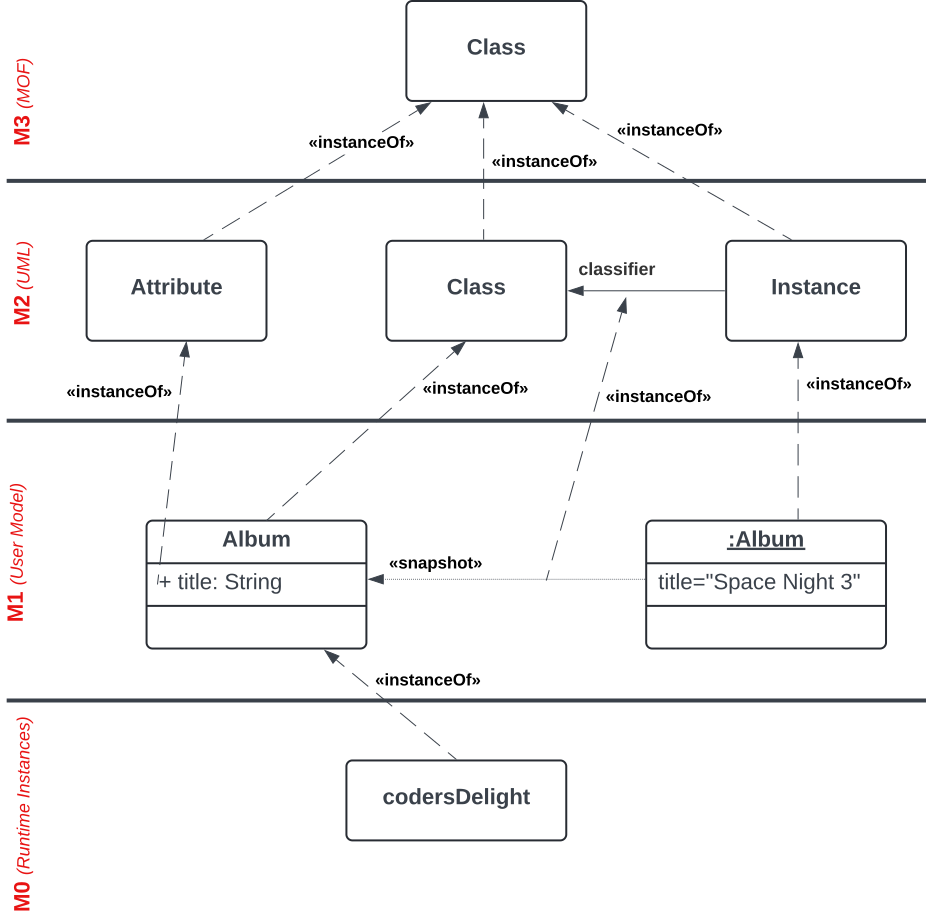
\includegraphics[scale=0.4]{part three/Einführung/img/metamodel}
    \caption{Beispiel für die verschiedenen Schichten der Metamodell Hierarchie.
        In der original Abbildung sind die Pfeilspitzen offen. (Quelle: in Anlehnung an S. 20, Figure 7.8, \url{https://www.omg.org/spec/UML/2.4.1/Infrastructure/PDF}, abgerufen 01.05.2024}
    \label{fig:metamodel-cc}
\end{figure}

\clearpage


\section{Strukturdiagramme}

\begin{tcolorbox}[title=Strukturdiagramme]
    In den \textbf{Strukturdiagrammen} werden \textbf{statische Strukturaspekte} eines Systems betrachtet.
    Für eine Systemmodellierung können alle dieser 6 Diagramme verwendet werden.

    \begin{itemize}
        \item \textbf{Klassendiagramm}: Das \textbf{Klassendiagramm} wird verwendet, um ein objektorientiertes System zu beschreiben.
        \item \textbf{Paketdiagramm}: Ein \textbf{Paketdiagramm} zeigt die Pakete eines Systems und deren Beziehungen.
        \item \textbf{Komponentendiagramm}: Stellt Komponenten oder auch \textit{Subsysteme} mit definierten Interfaces dar, um bspw. \textbf{Architekturdesign} darzustellen.
        \item \textbf{Verteilungsdiagramm}: Beschreibt eine Menge von Knoten, die die \textit{Ausführungsarchitektur} eines Systems definieren können, wobei Knoten i.d.R. \textit{Geräte} oder \textit{Softwareablaufumgebungen repräsentieren}.
        \item \textbf{Kompositionsstrukturdiagramm}: Stellt die \textbf{Komposition} von \textit{Systemstrukturen} (Klassen, Komponenten, Gesamtsystem) in einem bestimmten \textit{Kontext} mit einem bestimmten \textit{Ziel} dar (vgl. \cite[9]{Buh09}).
        \item \textbf{Objektdiagramm}: Momentaufnahme eines Systems zu genau einem \textit{Zeitpukt} während der Ausführung
    \end{itemize}

\end{tcolorbox}
\clearpage

\section{Verhaltensdiagramme}

\begin{tcolorbox}[title=Verhaltensdiagramme]
    \textbf{Verhaltensdiagramme} stellen \textit{Dynamik}, \textit{interne Abläufe} und das \textit{Zusammenspiel} der Systemteile dar, um eine Spezifikation zu vervollständigen.

    \begin{itemize}
        \item \textbf{Anwendungsfalldiagramm}: Dienen zur \textit{Spezifizierung} und \textit{Formalisierung} von \textit{Systemanforderungen}, unter Berücksichtigung von \textbf{Akteuren}, \textbf{Systemen} und \textbf{Anwendungsfällen}
        \item \textbf{Zustandsdiagramm}: Auch \textbf{Zustandsautomaten}; zeigen für ein einzelnes Objekt Zustandsänderungen während der Lebenszeit
        \item \textbf{Aktivitätsdiagramme}: Werden zur Modellierung von \textit{Kontroll}- oder \textit{Objektflüssen} oder zur Darstellung von \textit{Programmlogik} genutzt.
        \item \textbf{Interaktionsdiagramme}: Stellen das Zusammenspiel mehrerer Kommunikationspartner dar.
        Es gibt unterschiedliche Typen von Interaktionsdiagrammen, die Interaktionen auf verschiedenen \textit{Abstraktionsebenen} modellieren:
        \begin{itemize}
            \item \textbf{Sequenzdiagramm}: Zeigt den Verlauf einer Interaktion in zwei Dimensionen, \textit{Kommunikationspartner} und die Nachrichten in ihrer \textit{zeitlichen Abfolge}
            \item \textbf{Kommunikationsdiagramm}: hebt die Kommunikationsbeziehungen zwischen den Partnern hervor
            \item \textbf{Timing Diagramm}: hebt die zeitlichen Aspekte einer Interaktion hervor
            \item \textbf{Interaktionsüberblickdiagramm}: Spezialfall des \textbf{Aktivitätsdiagramms} - statt Aktionen und Aktivitäten können das \textbf{Sequenz}-, \textbf{Kommunikations}- und das \textbf{Timing}-Diagramm als Knoten verwendet werden.
        \end{itemize}
        Alle verwenden dieselben Grundelemente: \textit{Lebenslinien} der Akteure und Nachrichten, die zwischen diesen ausgetauscht werden.
    \end{itemize}
\end{tcolorbox}

\clearpage


\section{Klassendiagramm}

\begin{tcolorbox}[title=Klassendiagramm]
    Das \textbf{Klassendiagramm} beschreibt die Klassen eines Systems und die statischen Beziehungen zwischen ihnen.\\
    Sie werden in Form von Domainklassen bei der \textbf{Analyse} und als detaillierte Entwürfe von Systemklassen als \textit{Blueprint} im \textbf{gesamten Entwicklungsprozess} eingesetzt.

\end{tcolorbox}
\clearpage


\section{Assoziationsklasse (Attributierte Assoziation)}

\begin{tcolorbox}[title=Assoziationsklasse (Attributierte Assoziation)]
Eine \textbf{Assoziationsklasse} erlaubt das Hinzufügen von Operationen und Attributen zu einer Assoziation (\cite[43]{Buh09}).\\
Assoziationsklassen werden in der \textbf{Analyse} in Modellen verwendet und in dem \textbf{Entwurf} in eigenständige Klassen transformiert.\\

\noindent
Assoziationsklassen werden in der \textbf{Analyse} in Modellen verwendet und in dem \textbf{Entwurf} in eigenständige Klassen transformiert.

\blockquote[{\cite[277]{Oes05}}]{
    Eine attributierte Assoziation ist immer dann nahe liegend, wenn Attribute oder Operationen gefunden werden, die weder der einen noch der anderen Klasse zugeordnet werden können, weil sie nämlich Eigenschaften der Beziehung selbst sind.
}.\\

Bei einer attributierten Assoziation dürfen zwei beteiligte Objekte maximal nur eine Beziehung zueinander haben (vgl.~\cite[277]{Oes05})\footnote{
    \textit{Ostereich} führt dies ebenda auf Seite 278 weiter aus, in dem er beschreibt, wie eine attributierte Assoziation für ein \textit{Beschäftigtenverhältnis} zwischen \textit{Mitarbeiter} und \textit{Unternehmen} modelliert wird. Dabei wird davon ausgegangen, dass ein \textit{Mitarbeiter} nur über \textit{ein} Arbeitsverhältnis mit einem \textit{Unternehmen} in Beziehung stehen kann. Bestehen mehrere Arbeitsverhältnisse (\textit{Mitarbeiter} hat zu unterschiedlichen Zeitpunkten für das \textit{Unternehmen} gearbeitet), kann die attributierte Assoziation nicht verwendet werden.\\

\noindent
Wird eine attributierte Assoziation in eine gewöhnliche Assoziation transformiert, muss darauf geachtet werden, die Multiplizitäten richtig zu setzen (s. Abbildung~\ref{fig:assoziationsklasse}).
\end{tcolorbox}

\begin{figure}
    \centering
    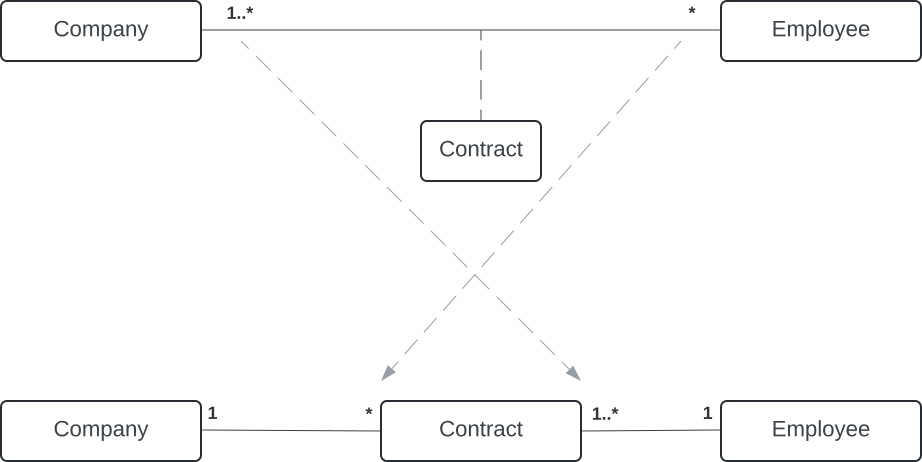
\includegraphics[scale=0.4]{part three/Klassendiagramme - Erweiterte Konzepte und Paketdiagramme/img/assoziationsklasse}
    \caption{Darstellung einer Assoziation mit Hilfe einer Assoziationsklasse (oben) sowie Transformation in gewöhnliche Assoziationen (unten). (Quelle: in Anlehnung an \cite[279, Abb. 4.4-11]{Oes05})}
    \label{fig:assoziationsklasse-cc}
\end{figure}

\clearpage


\section{Sequenzdiagramme}

\begin{tcolorbox}[title=Sequenzdiagramme]
    \textbf{Sequenzdiagramme} stellen Verhalten auf der Ebene einer Interaktion dar.\\
    In der Phase des Klassendesigns werden die Teilnehmer der Interaktionen bestimmt, weshalb Sequenzdiagramme oft in dieser Phase genutzt werden.\\
    In der \textbf{Analysephase} können Sequenzdiagramme eingesetzt werden, um die Kommunikation der bis dahin ausgemachten \textbf{Geschäftsobjekte} zu modellieren, oder um \textbf{Anwendungsfälle} weiter zu spezifizieren.
\end{tcolorbox}
\clearpage

\section{Aggregation}

\begin{tcolorbox}[title=Aggregation]
    Eine \textbf{Aggregation} ist in ihrer \semantischen Aussage unscharf (vgl.~\cite[40]{Buh09}).\\
    Sie beschreibt eine \textit{Ganzes}-\textit{Teile}-Beziehung, aber die \textit{Teile} können zu mehreren verschiedenen \textit{Ganzen} gehören.\\
    Außerdem kann ein Teil dem \textit{Ganzen} jederzeit wieder entnommen werden und das \textit{Ganze} ist nicht verantwortlich für das Erstellen der \textit{Teile}, weshalb Implementierungen beim Hinzufügen von Teilen oft schon fertige Objekte erwarten, die jeweils eines der \textit{Teile} repräsentieren.\\
    Aggregationsbeziehungen werden durch eine nicht-gefüllte Raute an der Seite der Klasse, die das Ganze repräsentiert, dargestellt.
\end{tcolorbox}
\clearpage

\section{Komposition}

\begin{tcolorbox}[title=Komposition]
    Bei einer \textbf{Komposition} handelt es sich um eine \textit{Ganzes}-\textit{Teile}-Beziehung, bei der das \textit{Ganze} verantwortlich für die Erstellung und Beseitigung der \textit{Teile} ist.
    Außerdem sind die \textit{Teile} an die \textbf{Existenz} des \textit{Ganzen} gebunden.\\
    \textit{Teile} gehören immer zu \textit{genau einem} \textit{Ganzen}.\\
    Eine Komposition wird dargestellt durch eine gefüllte Raute an der Klassenbox, die das \textit{Ganze} repräsentiert.
\end{tcolorbox}
\clearpage

\section{Paketdiagramm}

\begin{tcolorbox}[title=Komposition]
    \textbf{Paketdiagramme} zeigen Pakete und ihre Abhängigkeiten und werden in frühen Designphasen genutzt, um Strukturen (großer Systeme) aufzuzeigen.\\

    \noindent
    Elemente sollten so in Paketen gruppiert werden, dass ihr \textbf{funktionaler Zusammenhalt} (\textit{Kohäsion}, s. Abschnitt~\ref{subsec:hohe-kohasion}) klar wird.\\
    Hierdurch kann vermieden werden, dass Änderungen einer Klasse eines Paketes auch Änderungen außerhalb des Paketes erfordern.\\
    Außerdem erhöht sich die Wahrscheinlichkeit, dass einzelne Pakete als solche in anderen Projekten wiederverwendet werden können.\\

    \noindent
    In Paketdiagrammen können Beziehungen über folgende Schlüsselwörter deutlich gemacht werden:

    \begin{itemize}
        \item \guillemotleft import\guillemotright
        \item[] $\rightarrow$ \textbf{public-Import} zwischen Quell- und Zielpaket; Quellpaket kann die öffentlichen Elemente des Zielpaketes unter Verwendung des unqualifizierten und des qualifizierten Namens verwenden; die importierten Elemente sind auch für Pakete sichtbar, die das Quellpaket importieren
        \item \guillemotleft access\guillemotright
        \item[] $\rightarrow$ \textbf{privater Import} zwischen Quell- und Zielpaket; Zugriff auf Elemente des importierten Paketes ohne qualifizierenden Namen möglich; der Import eines Paketes in \textbf{Java} entspricht der \guillemotleft access\guillemotright-Beziehung
        \item \guillemotleft merge\guillemotright
        \item[] $\rightarrow$ Bei einem \textbf{merge} werden Elemente eines Zielpaketes in das Quellpaket
   \end{itemize}
\end{tcolorbox}
\clearpage

\section{Anwendungsfalldiagramm}

\begin{tcolorbox}[title=Anwendungsfalldiagramm]
    Die \textbf{Anwendungsfallanalyse} wird im Rahmen der \textbf{Anforderungsspezifikation} eingesetzt.\\

    \noindent
    Anwendungsfalldiagramme sind das am häufigsten eingesetzte Mittel zur Aufnahme und Darstellung von \textbf{Anforderungen}.\\
    Sie beschreiben selbst kein Verhalten und keine Abläufe, sondern zeigen nur die Zusammenhänge der an Anwendungsfällen beteiligten Modellelemente und sind somit ein Hilfsmittel zur Anforderungsermittlung und Verwaltung.\\

    \noindent
    Zu den wichtigsten Schritten einer Anwendungsfallanalyse gehören:
    \begin{enumerate}
        \item Akteure identifizieren
        \item Anwendungsfälle identifizieren
        \item Beschreiben der Akteure und Anwendungsfälle
        \item Identifizieren von \textit{Schlüsselobjekten}, die das System verwaltet
        \item Identifizieren der wichtigsten Anwendungsfälle (Priorisierung)
        \item detailliertere Beschreibung der Anwendungsfälle
        \item Strukturierung des Anwendungsfalldiagramms
    \end{enumerate}

    \noindent
    Anwendungsfälle beschreiben das \textbf{Szenario} der Nutzung, und nicht Features des Systems.
\end{tcolorbox}

\clearpage

\input{chapters/Anhang/CheatSheets/SE3/Aktivitätsdiagramm}
\clearpage

\section{Zustandsautomat}

\begin{tcolorbox}[title=Zustandsautomat]
    Mit \textbf{Zustandsautomaten} kann das \textit{Verhalten} von Systemen modelliert werden, wobei die \textit{Reaktionen} des Systems im Mittelpunkt stehen, und nicht die \textit{Aktionen}, wie bspw. bei den \textbf{Aktivitätsdiagrammen}.\\

    \noindent
        Ein \textbf{Zustandsautomat} kann den \textit{Lebensweg} eines Objektes modellieren, weshalb Zustandsautomaten oft im \textbf{Entwurf} als Ergänzung zu den \textbf{Klassendiagrammen} eingesetzt werden.
\end{tcolorbox}

\begin{figure}
    \centering
    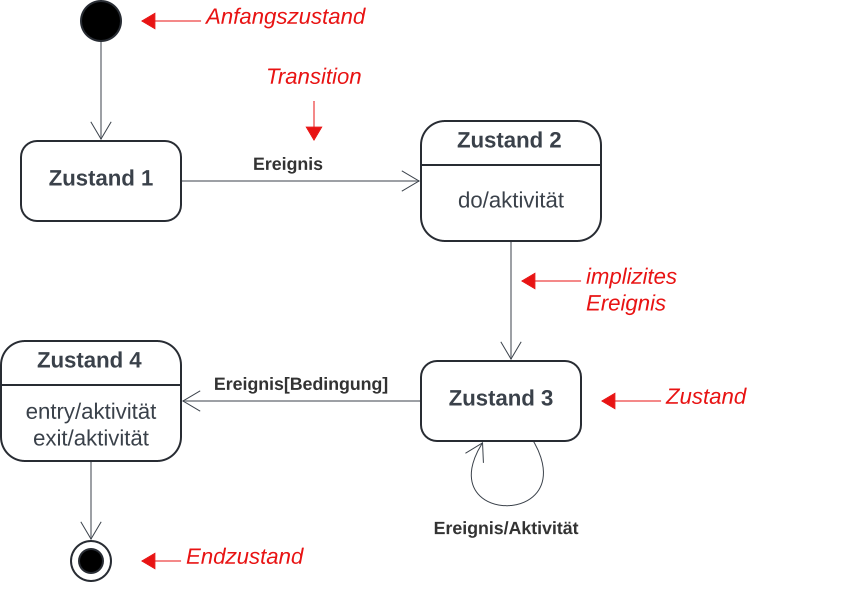
\includegraphics[scale=0.4]{part three/Zustandsautomaten/img/statechartdiagramnotation}
    \caption{Elemente eines einfachen Zustandsautomaten. Eine Transitionen wird durch ein \textbf{Ereignis} ausgelöst, das ein \textit{Signal}, ein \textit{Operationsaufruf} oder auch eine bestimmte \textit{Attributänderung} sein kann. (Quelle: in Anlehnung an \cite[90, Abb. 2.11-6]{Bal05})}
    \label{fig:statechartdiagramnotation-cc}
\end{figure}

\begin{minted}[fontsize=\small]{java}
// Beispiel für eine Implementierung eines
// Parkscheinautomaten als Zustandsautomat in Java
class Parkscheinautomat {

  // zustände
  private final int BEREIT = 0;
  private final int ZAHLUNG = 1;
  private final int ABBRUCH = 2;
  private final int BELEG   = 3;

  // Zustand; wird initial beim Starten
  // des Automaten gesetzt
  private int zustand;

  // Methoden lösen Aktionen beim Eintritt
  // in die jeweiligen Zustände aus
  private int zahlung() {
    // verarbeiten
    // danach neuen Zustand zurückliefern...
    ...
    return BEREIT;
  }

   ...

  private void bereit() {
    while (true) {
      // eingabe überprüfen und
      // ggf. Zustandswechsel auslösen:
      // Zustand als Attribut setzen
      ...
    }
  }

  public void start() {
    zustand = BEREIT;

    while(true) {
      switch (zustand) {
        case BEREIT:
          zustand = bereit();
        // ... weiteres Verhalten
        ...
      }
    }
  }
}
\end{minted}
\clearpage
	

\section{Inhalt SE3}

\section*{1. Übersicht UML}

\subsection*{Lernziele}
\begin{itemize}
    \item einen Einblick in den Sprachaufbau der UML 2.0 gewinnen
    \item einen Überblick über die Diagramme der UML 2.0 und deren Zweck haben
\end{itemize}

\subsection*{Zusammenfassung}
\begin{itemize}
    \item Die \textbf{UML} ist eine weit verbreitete Modellierungssprache zur Modellierung objektorientierter Softwaresysteme.
    \item Die UML 2.0 Spezifikation besteht aus vier Teilen:
    \begin{enumerate}
        \item \textbf{Superstructure}: Diagrammtypen
        \item \textbf{Infrastructure}: Modellierungskonzepte
        \item \textbf{OCL}: formale Sprache zur Formulierung von Einschränkungen
        \item \textbf{Diagram Interchange}: Austauschformate
    \end{enumerate}
    \item Die UML kann im \textbf{Sketching} oder \textbf{Blueprint Modus} eingesetzt werden, oder als Grundlage für \textbf{automatische Codegenerierung}
    \item Die UML ist an keinen speziellen Entwicklungsprozess gebunden
\end{itemize}

\section*{2. Klassendiagramme}

\subsection*{Lernziele}
\begin{itemize}
    \item wissen, wie Klassendiagramme im Entwicklungsprozess eingesetzt werden
    \item Klassendiagramme für Analyse- und Designentscheidungen einsetzen können
    \item die wichtigsten Modellierungskonzepte kennen
    \item sinnvolle Klassendiagramme erstellen und Java-Implementierungen ableiten können
    \item Klassendiagramme aus Java Quellcode erzeugen können
\end{itemize}

\subsection*{Zusammenfassung}

\begin{itemize}
    \item \textbf{Klassendiagramme} dienen zur \textbf{strukturellen Darstellung} von Softwaresystemen
    \item hierbei werden Klassen und \textbf{Beziehungen} zwischen Klassen dargestellt
    \item Properties können durch die \textbf{Attribut}- oder \textbf{Assoziationsnotation} modelliert werden
    \item Operationen werden als separate Zeile in ihrem Compartment dargestellt
    \item im Klassendiagramm können auch \textbf{Generalisierungsbeziehungen} modelliert werden
    \item \textbf{Abhängigkeitsbeziehungen} drücken ein Verhältnis zwischen \textbf{Client} und \textbf{Supplier} aus
\end{itemize}

\section*{3. Objektorientierter Entwurf}

\subsection*{Lernziele}
\begin{itemize}
    \item das Wesen einer Interaktion kennen
    \item wissen, wie Sequenzdiagramme im Entwicklungsprozess eingesetzt werden
    \item Sequenzdiagramme für Analyse- und Designentscheidungen sowie zur Darstellung von Kontrollflüssen einsetzen können
    \item die wichtigsten Modellierungskonzepte kennen
    \item sinnvolle Sequenzdiagramme erstellen und Java-Implementierungen ableiten können
    \item Sequenzdiagramme aus Java Quellcode erzeugen können
\end{itemize}

\subsection*{Zusammenfassung}

\begin{itemize}
    \item Sequenzdiagramme sind \textbf{Verhaltensdiagramme}
    und können im gesamten Entwicklungszyklus zur Modellierung von Interaktionen angewendet werden
    \item Interaktionen bestehen im Wesentlichen aus dem Nachrichtenaustausch zwischen verschiedenen Kommunikationspartnern
    \item in den meisten Fällen wird die Kommunikation von Objekten von Klassen modelliert, aber es können auch Teilnehmer auf anderen Ebenen modelliert werden
    \item gewöhnlich gibt ein Sequenzdiagramm einen \textbf{Anwendungsfall} (\textit{Szenario}) wieder
    \item sie dienen nicht dazu, um Zustandsänderungen darzustellen (hierfür werden Zustandsdiagramme verwendet)
    \item Sequenzdiagramme sind \textit{nicht} gut geeignet für die Darstellung von
    \begin{itemize}
        \item nebenläufigem Verhalten (\textit{asynchrone} Nachrichten, \textit{kombiniertes Fragment})
        \item Schleifen und alternativem Verhalten (\textit{kombinierte Fragmente})
        \item[] $\rightarrow$  für beide Fälle sind \textbf{Aktivitätsdiagramme} besser geeignet
    \end{itemize}
\end{itemize}

\section*{4. Klassendiagramme - Erweiterte Konzepte und Paketdiagramme}

\subsection*{Lernziele}
\begin{itemize}
    \item erweiterte Modellierungskonzepte in Klassendiagrammen für den Detailentwurf von Systemen kennen
    \item die Konsequenzen dieser Konzepte in der Implementierung kennen
    \item wissen, wie Paketdiagramme im Entwicklungsprozess eingesetzt werden
    \item die Modellierungskonzepte in Paketdiagrammen kennen
    \item anhand von Paketdiagrammen Software-Architekturen gestalten und bewerten können
\end{itemize}

\subsection*{Zusammenfassung}

\begin{itemize}
    \item Die vorgestellten erweiterten Konzepte werden vor allem im \textbf{Feinentwurf} von Klassenstrukturen eingesetzt.
    \item Generell gilt, dass die Spezifikationen von Objekten und Properties nur so detailliert ausgeführt werden sollen, wie nötig: Sind Details für das Verständnis unnötig, sollte darauf verzichtet werden.
    \item \textbf{Generalisierungsbeziehungen} sollten grundsätzlich modelliert werden.
    \item Ist eine \textbf{Komposition} statt einer Generalisierung für den Sachverhalt möglich, sollte diese verwendet werden: ``Favor object composition over inheritance.`` (\cite[19 f.]{GHJV94})
    \item \textbf{Kompositionsbeziehungen} geben eindeutige Impulse für eine Implementierung, \textbf{Aggregationsbeziehungen} sind in ihrer semantischen Aussage nicht sehr eindeutig
    \item \textbf{Assoziationsklassen} sind in ihrer frühen Designphase empfehlenswert, die Realisierung (mit {bspw.} Java) erfordert aber eine Transformation in eine volle Klasse, wobei die Multiplizitäten angepasst werden müssen
    \item Elemente können in \textbf{Paketen} zusamengefasst und unter einem gemeinsamen Namensraum gruppiert werden
\end{itemize}

\section*{4. Anwendungsfalldiagramm (Use-Case-Diagramm)}

\subsection*{Lernziele}
\begin{itemize}
    \item wissen, wie die Anwendungsfallanalyse im Rahmen der Anforderungsspezifikation eingesetzt wird
    \item Prozessschritte der Anwendungsfallanalyse beherrschen
    \item die wichtigsten Modellierungskonzepte in Anwendungsfalldiagrammen kennen
    \item den Aufbau einer Anwendungsfallbeschreibung kennen
\end{itemize}

\subsection*{Zusammenfassung}

\begin{itemize}
    \item \textbf{Anwendungsfalldiagramme} besitzen eine einfache Notation, um \textbf{Akteure} und \textbf{Anwendungsfälle} eines \textbf{Systems} grafisch darzustellen
    \item auf Basis eines Anwendungsfalldiagramms lässt sich ermitteln, ob die Anwendungsfälle gewünschtes Verhalten realisieren bzw. Beziehungen zu einem oder mehreren Akteuren haben
    \item Anwendungsfälle und Akteure \textit{müssen} zusätzlich textlich beschrieben werden
\end{itemize}

\section*{5. Aktivitätsdiagramme}

\subsection*{Lernziele}
\begin{itemize}
    \item wissen, wie Aktivitätsdiagramme im Rahmen der Verhaltensanalyse in verschiedenen Prozessphasen eingesetzt werden können
    \item die wichtigsten Modellierungskonzepte in Aktivitätsdiagrammen kennen
    \item Aktivitätsdiagramme interpretieren, erstellen und implementieren können
\end{itemize}

\subsection*{Zusammenfassung}

\begin{itemize}
    \item \textbf{Aktivitätsdiagramme} gehören zu den \textbf{Verhaltensdiagrammen} und können im \textit{gesamten} \textbf{Entwicklungsprozess} eingesetzt werden
    \item durch ein Aktivitätsdiagramm kann gezeigt werden, wie \textbf{Verhalten} realisiert wird
    \item es können mehrere \textbf{Aktivitäten} dargestellt werden
    \item \textbf{Aktivitätskanten} und \textbf{Aktivitätsknoten} werden zur Beschreibung von Verhalten verwendet
\end{itemize}

\section*{5. Zustandsautomaten}

\subsection*{Lernziele}
\begin{itemize}
    \item wissen, wie Zustandsdiagramme im Rahmen der Verhaltensanalyse einzelner Objekte eingesetzt werden können
    \item die wichtigsten Modellierungskonzepte in Zustandsdiagrammen kennen
    \item Zustandsdiagramme interpretieren, erstellen und implementieren können
\end{itemize}

\subsection*{Zusammenfassung}

\begin{itemize}
    \item Das \textbf{Zustandsdiagramm} gehört wie das \textbf{Aktivitätsdiagramm} zu den \textbf{Verhaltensdiagrammen}.
    \item Ein Zustandsdiagramm zeigt den \textbf{Lebensweg} eines \textbf{Objektes}.
    \item \textbf{Attributwerte} bestimmen den Zustand eines Objektes.
    \item \textbf{Transitionen} zwischen Zuständen werden durch \textbf{Guards} und \textbf{Events} gesteuert.
    \item Während der Transitionen können \textbf{Effekte} (\textit{Aktivitäten}) realisiert werden.
    \item Die Modellierung \textbf{zusammengesetzter Zustände} ist ebenfalls möglich.
    \item Für die Darstellung \textbf{paralleler} oder  \textbf{konkurrierender} Abläufe können \textbf{Regionen} modelliert werden.
\end{itemize}
\clearpage


\section{UML Modellierung}

\begin{tcolorbox}[title=UML Modellierung]
    \textbf{Modelle} haben die Aufgabe, den Bezug zum Original (Programm, Softwaresystem) herzustellen, sowie zu der \textit{Anwendungsumgebung}.\\
    Ein \textbf{Modell} enthält alle \textbf{Modellelemente}, die zur Beschreibung eines Softwaresystems nötig sind.\\

    \noindent
    Ein \textbf{Modellelement} wird als Element in einem UML Modell von einem Benutzer erstellt und auf verschiedenen \textbf{Diagrammen} (Struktur-/Verhaltensdiagrammen) platziert, und wird durch die \textbf{UML Modellierungskonzepte} als Metaklasse des \textbf{Metamodells} der UML beschrieben: \textbf{Modellelemente} werden aus Modellierungskonzepten instanziiert.\\

    \noindent
       Das \textbf{UML Metamodell} regelt, in welchem Zusammenhang \textbf{UML Modellierungskonzepte} in Modellen auftreten dürfen, und welche Eigenschaften und Beziehungen zu anderen Sprachelementen zulässig sind.\\

       \noindent
       Die im \textbf{Metamodell} verwendeten Erklärungen basieren auf einer abstrakten Syntax, für deren Beschreibung eine Untermenge (\textit{Klassendiagramme}) der UML verwendet wird.\\
        Die \textbf{Semantik} der Modellierungskonzepte wird textlich beschrieben, zur Formalisierung von Regeln für die syntaktische Korrektheit wird die \textbf{OCL} (\textit{Object Constraint Language}) verwendet.
\end{tcolorbox}

\begin{figure}
    \centering
    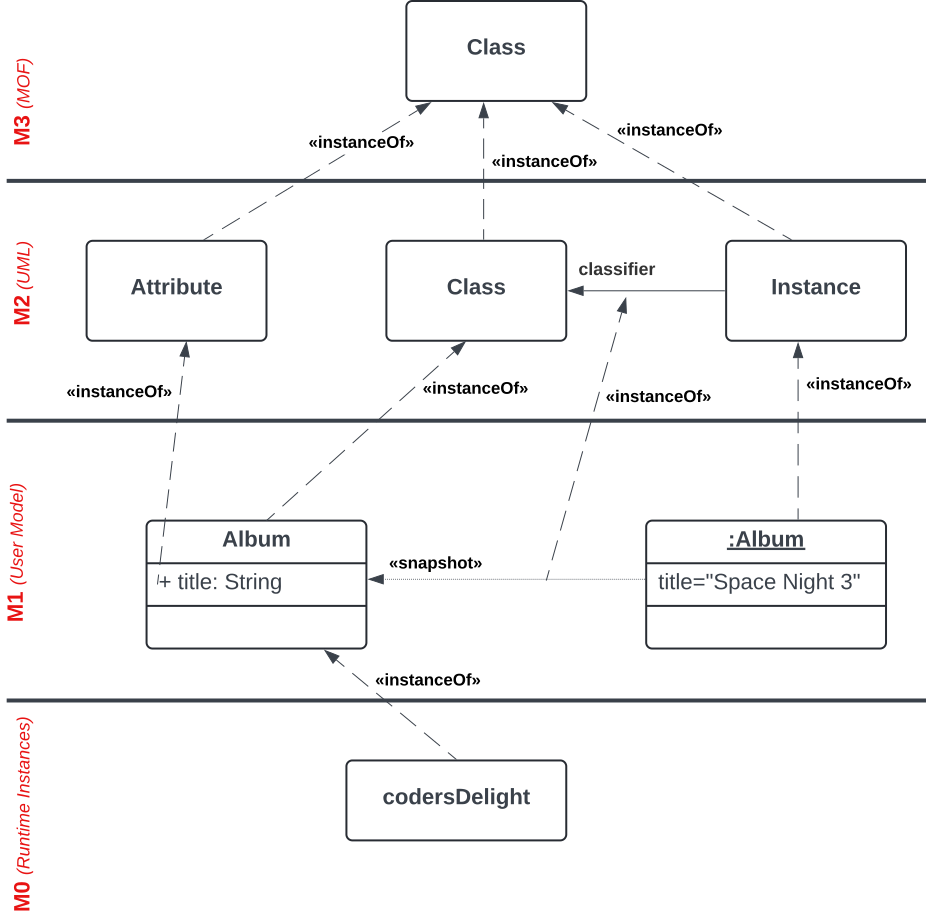
\includegraphics[scale=0.4]{part three/Einführung/img/metamodel}
    \caption{Beispiel für die verschiedenen Schichten der Metamodell Hierarchie.
        In der original Abbildung sind die Pfeilspitzen offen. (Quelle: in Anlehnung an S. 20, Figure 7.8, \url{https://www.omg.org/spec/UML/2.4.1/Infrastructure/PDF}, abgerufen 01.05.2024}
    \label{fig:metamodel-cc}
\end{figure}

\clearpage


\section{Strukturdiagramme}

\begin{tcolorbox}[title=Strukturdiagramme]
    In den \textbf{Strukturdiagrammen} werden \textbf{statische Strukturaspekte} eines Systems betrachtet.
    Für eine Systemmodellierung können alle dieser 6 Diagramme verwendet werden.

    \begin{itemize}
        \item \textbf{Klassendiagramm}: Das \textbf{Klassendiagramm} wird verwendet, um ein objektorientiertes System zu beschreiben.
        \item \textbf{Paketdiagramm}: Ein \textbf{Paketdiagramm} zeigt die Pakete eines Systems und deren Beziehungen.
        \item \textbf{Komponentendiagramm}: Stellt Komponenten oder auch \textit{Subsysteme} mit definierten Interfaces dar, um bspw. \textbf{Architekturdesign} darzustellen.
        \item \textbf{Verteilungsdiagramm}: Beschreibt eine Menge von Knoten, die die \textit{Ausführungsarchitektur} eines Systems definieren können, wobei Knoten i.d.R. \textit{Geräte} oder \textit{Softwareablaufumgebungen repräsentieren}.
        \item \textbf{Kompositionsstrukturdiagramm}: Stellt die \textbf{Komposition} von \textit{Systemstrukturen} (Klassen, Komponenten, Gesamtsystem) in einem bestimmten \textit{Kontext} mit einem bestimmten \textit{Ziel} dar (vgl. \cite[9]{Buh09}).
        \item \textbf{Objektdiagramm}: Momentaufnahme eines Systems zu genau einem \textit{Zeitpukt} während der Ausführung
    \end{itemize}

\end{tcolorbox}
\clearpage

\section{Verhaltensdiagramme}

\begin{tcolorbox}[title=Verhaltensdiagramme]
    \textbf{Verhaltensdiagramme} stellen \textit{Dynamik}, \textit{interne Abläufe} und das \textit{Zusammenspiel} der Systemteile dar, um eine Spezifikation zu vervollständigen.

    \begin{itemize}
        \item \textbf{Anwendungsfalldiagramm}: Dienen zur \textit{Spezifizierung} und \textit{Formalisierung} von \textit{Systemanforderungen}, unter Berücksichtigung von \textbf{Akteuren}, \textbf{Systemen} und \textbf{Anwendungsfällen}
        \item \textbf{Zustandsdiagramm}: Auch \textbf{Zustandsautomaten}; zeigen für ein einzelnes Objekt Zustandsänderungen während der Lebenszeit
        \item \textbf{Aktivitätsdiagramme}: Werden zur Modellierung von \textit{Kontroll}- oder \textit{Objektflüssen} oder zur Darstellung von \textit{Programmlogik} genutzt.
        \item \textbf{Interaktionsdiagramme}: Stellen das Zusammenspiel mehrerer Kommunikationspartner dar.
        Es gibt unterschiedliche Typen von Interaktionsdiagrammen, die Interaktionen auf verschiedenen \textit{Abstraktionsebenen} modellieren:
        \begin{itemize}
            \item \textbf{Sequenzdiagramm}: Zeigt den Verlauf einer Interaktion in zwei Dimensionen, \textit{Kommunikationspartner} und die Nachrichten in ihrer \textit{zeitlichen Abfolge}
            \item \textbf{Kommunikationsdiagramm}: hebt die Kommunikationsbeziehungen zwischen den Partnern hervor
            \item \textbf{Timing Diagramm}: hebt die zeitlichen Aspekte einer Interaktion hervor
            \item \textbf{Interaktionsüberblickdiagramm}: Spezialfall des \textbf{Aktivitätsdiagramms} - statt Aktionen und Aktivitäten können das \textbf{Sequenz}-, \textbf{Kommunikations}- und das \textbf{Timing}-Diagramm als Knoten verwendet werden.
        \end{itemize}
        Alle verwenden dieselben Grundelemente: \textit{Lebenslinien} der Akteure und Nachrichten, die zwischen diesen ausgetauscht werden.
    \end{itemize}
\end{tcolorbox}

\clearpage


\section{Klassendiagramm}

\begin{tcolorbox}[title=Klassendiagramm]
    Das \textbf{Klassendiagramm} beschreibt die Klassen eines Systems und die statischen Beziehungen zwischen ihnen.\\
    Sie werden in Form von Domainklassen bei der \textbf{Analyse} und als detaillierte Entwürfe von Systemklassen als \textit{Blueprint} im \textbf{gesamten Entwicklungsprozess} eingesetzt.

\end{tcolorbox}
\clearpage


\section{Assoziationsklasse (Attributierte Assoziation)}

\begin{tcolorbox}[title=Assoziationsklasse (Attributierte Assoziation)]
Eine \textbf{Assoziationsklasse} erlaubt das Hinzufügen von Operationen und Attributen zu einer Assoziation (\cite[43]{Buh09}).\\
Assoziationsklassen werden in der \textbf{Analyse} in Modellen verwendet und in dem \textbf{Entwurf} in eigenständige Klassen transformiert.\\

\noindent
Assoziationsklassen werden in der \textbf{Analyse} in Modellen verwendet und in dem \textbf{Entwurf} in eigenständige Klassen transformiert.

\blockquote[{\cite[277]{Oes05}}]{
    Eine attributierte Assoziation ist immer dann nahe liegend, wenn Attribute oder Operationen gefunden werden, die weder der einen noch der anderen Klasse zugeordnet werden können, weil sie nämlich Eigenschaften der Beziehung selbst sind.
}.\\

Bei einer attributierten Assoziation dürfen zwei beteiligte Objekte maximal nur eine Beziehung zueinander haben (vgl.~\cite[277]{Oes05})\footnote{
    \textit{Ostereich} führt dies ebenda auf Seite 278 weiter aus, in dem er beschreibt, wie eine attributierte Assoziation für ein \textit{Beschäftigtenverhältnis} zwischen \textit{Mitarbeiter} und \textit{Unternehmen} modelliert wird. Dabei wird davon ausgegangen, dass ein \textit{Mitarbeiter} nur über \textit{ein} Arbeitsverhältnis mit einem \textit{Unternehmen} in Beziehung stehen kann. Bestehen mehrere Arbeitsverhältnisse (\textit{Mitarbeiter} hat zu unterschiedlichen Zeitpunkten für das \textit{Unternehmen} gearbeitet), kann die attributierte Assoziation nicht verwendet werden.\\

\noindent
Wird eine attributierte Assoziation in eine gewöhnliche Assoziation transformiert, muss darauf geachtet werden, die Multiplizitäten richtig zu setzen (s. Abbildung~\ref{fig:assoziationsklasse}).
\end{tcolorbox}

\begin{figure}
    \centering
    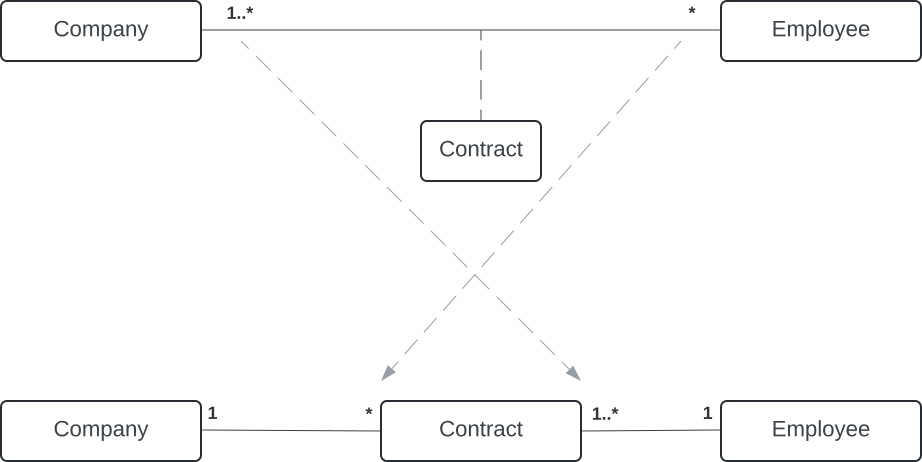
\includegraphics[scale=0.4]{part three/Klassendiagramme - Erweiterte Konzepte und Paketdiagramme/img/assoziationsklasse}
    \caption{Darstellung einer Assoziation mit Hilfe einer Assoziationsklasse (oben) sowie Transformation in gewöhnliche Assoziationen (unten). (Quelle: in Anlehnung an \cite[279, Abb. 4.4-11]{Oes05})}
    \label{fig:assoziationsklasse-cc}
\end{figure}

\clearpage


\section{Sequenzdiagramme}

\begin{tcolorbox}[title=Sequenzdiagramme]
    \textbf{Sequenzdiagramme} stellen Verhalten auf der Ebene einer Interaktion dar.\\
    In der Phase des Klassendesigns werden die Teilnehmer der Interaktionen bestimmt, weshalb Sequenzdiagramme oft in dieser Phase genutzt werden.\\
    In der \textbf{Analysephase} können Sequenzdiagramme eingesetzt werden, um die Kommunikation der bis dahin ausgemachten \textbf{Geschäftsobjekte} zu modellieren, oder um \textbf{Anwendungsfälle} weiter zu spezifizieren.
\end{tcolorbox}
\clearpage

\section{Aggregation}

\begin{tcolorbox}[title=Aggregation]
    Eine \textbf{Aggregation} ist in ihrer \semantischen Aussage unscharf (vgl.~\cite[40]{Buh09}).\\
    Sie beschreibt eine \textit{Ganzes}-\textit{Teile}-Beziehung, aber die \textit{Teile} können zu mehreren verschiedenen \textit{Ganzen} gehören.\\
    Außerdem kann ein Teil dem \textit{Ganzen} jederzeit wieder entnommen werden und das \textit{Ganze} ist nicht verantwortlich für das Erstellen der \textit{Teile}, weshalb Implementierungen beim Hinzufügen von Teilen oft schon fertige Objekte erwarten, die jeweils eines der \textit{Teile} repräsentieren.\\
    Aggregationsbeziehungen werden durch eine nicht-gefüllte Raute an der Seite der Klasse, die das Ganze repräsentiert, dargestellt.
\end{tcolorbox}
\clearpage

\section{Komposition}

\begin{tcolorbox}[title=Komposition]
    Bei einer \textbf{Komposition} handelt es sich um eine \textit{Ganzes}-\textit{Teile}-Beziehung, bei der das \textit{Ganze} verantwortlich für die Erstellung und Beseitigung der \textit{Teile} ist.
    Außerdem sind die \textit{Teile} an die \textbf{Existenz} des \textit{Ganzen} gebunden.\\
    \textit{Teile} gehören immer zu \textit{genau einem} \textit{Ganzen}.\\
    Eine Komposition wird dargestellt durch eine gefüllte Raute an der Klassenbox, die das \textit{Ganze} repräsentiert.
\end{tcolorbox}
\clearpage

\section{Paketdiagramm}

\begin{tcolorbox}[title=Komposition]
    \textbf{Paketdiagramme} zeigen Pakete und ihre Abhängigkeiten und werden in frühen Designphasen genutzt, um Strukturen (großer Systeme) aufzuzeigen.\\

    \noindent
    Elemente sollten so in Paketen gruppiert werden, dass ihr \textbf{funktionaler Zusammenhalt} (\textit{Kohäsion}, s. Abschnitt~\ref{subsec:hohe-kohasion}) klar wird.\\
    Hierdurch kann vermieden werden, dass Änderungen einer Klasse eines Paketes auch Änderungen außerhalb des Paketes erfordern.\\
    Außerdem erhöht sich die Wahrscheinlichkeit, dass einzelne Pakete als solche in anderen Projekten wiederverwendet werden können.\\

    \noindent
    In Paketdiagrammen können Beziehungen über folgende Schlüsselwörter deutlich gemacht werden:

    \begin{itemize}
        \item \guillemotleft import\guillemotright
        \item[] $\rightarrow$ \textbf{public-Import} zwischen Quell- und Zielpaket; Quellpaket kann die öffentlichen Elemente des Zielpaketes unter Verwendung des unqualifizierten und des qualifizierten Namens verwenden; die importierten Elemente sind auch für Pakete sichtbar, die das Quellpaket importieren
        \item \guillemotleft access\guillemotright
        \item[] $\rightarrow$ \textbf{privater Import} zwischen Quell- und Zielpaket; Zugriff auf Elemente des importierten Paketes ohne qualifizierenden Namen möglich; der Import eines Paketes in \textbf{Java} entspricht der \guillemotleft access\guillemotright-Beziehung
        \item \guillemotleft merge\guillemotright
        \item[] $\rightarrow$ Bei einem \textbf{merge} werden Elemente eines Zielpaketes in das Quellpaket
   \end{itemize}
\end{tcolorbox}
\clearpage

\section{Anwendungsfalldiagramm}

\begin{tcolorbox}[title=Anwendungsfalldiagramm]
    Die \textbf{Anwendungsfallanalyse} wird im Rahmen der \textbf{Anforderungsspezifikation} eingesetzt.\\

    \noindent
    Anwendungsfalldiagramme sind das am häufigsten eingesetzte Mittel zur Aufnahme und Darstellung von \textbf{Anforderungen}.\\
    Sie beschreiben selbst kein Verhalten und keine Abläufe, sondern zeigen nur die Zusammenhänge der an Anwendungsfällen beteiligten Modellelemente und sind somit ein Hilfsmittel zur Anforderungsermittlung und Verwaltung.\\

    \noindent
    Zu den wichtigsten Schritten einer Anwendungsfallanalyse gehören:
    \begin{enumerate}
        \item Akteure identifizieren
        \item Anwendungsfälle identifizieren
        \item Beschreiben der Akteure und Anwendungsfälle
        \item Identifizieren von \textit{Schlüsselobjekten}, die das System verwaltet
        \item Identifizieren der wichtigsten Anwendungsfälle (Priorisierung)
        \item detailliertere Beschreibung der Anwendungsfälle
        \item Strukturierung des Anwendungsfalldiagramms
    \end{enumerate}

    \noindent
    Anwendungsfälle beschreiben das \textbf{Szenario} der Nutzung, und nicht Features des Systems.
\end{tcolorbox}

\clearpage

\input{chapters/Anhang/CheatSheets/SE3/Aktivitätsdiagramm}
\clearpage

\section{Zustandsautomat}

\begin{tcolorbox}[title=Zustandsautomat]
    Mit \textbf{Zustandsautomaten} kann das \textit{Verhalten} von Systemen modelliert werden, wobei die \textit{Reaktionen} des Systems im Mittelpunkt stehen, und nicht die \textit{Aktionen}, wie bspw. bei den \textbf{Aktivitätsdiagrammen}.\\

    \noindent
        Ein \textbf{Zustandsautomat} kann den \textit{Lebensweg} eines Objektes modellieren, weshalb Zustandsautomaten oft im \textbf{Entwurf} als Ergänzung zu den \textbf{Klassendiagrammen} eingesetzt werden.
\end{tcolorbox}

\begin{figure}
    \centering
    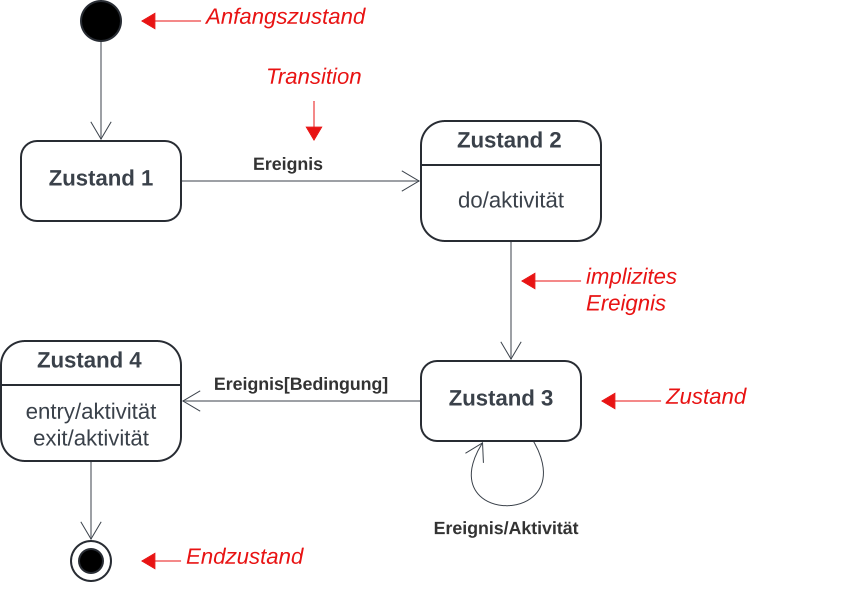
\includegraphics[scale=0.4]{part three/Zustandsautomaten/img/statechartdiagramnotation}
    \caption{Elemente eines einfachen Zustandsautomaten. Eine Transitionen wird durch ein \textbf{Ereignis} ausgelöst, das ein \textit{Signal}, ein \textit{Operationsaufruf} oder auch eine bestimmte \textit{Attributänderung} sein kann. (Quelle: in Anlehnung an \cite[90, Abb. 2.11-6]{Bal05})}
    \label{fig:statechartdiagramnotation-cc}
\end{figure}

\begin{minted}[fontsize=\small]{java}
// Beispiel für eine Implementierung eines
// Parkscheinautomaten als Zustandsautomat in Java
class Parkscheinautomat {

  // zustände
  private final int BEREIT = 0;
  private final int ZAHLUNG = 1;
  private final int ABBRUCH = 2;
  private final int BELEG   = 3;

  // Zustand; wird initial beim Starten
  // des Automaten gesetzt
  private int zustand;

  // Methoden lösen Aktionen beim Eintritt
  // in die jeweiligen Zustände aus
  private int zahlung() {
    // verarbeiten
    // danach neuen Zustand zurückliefern...
    ...
    return BEREIT;
  }

   ...

  private void bereit() {
    while (true) {
      // eingabe überprüfen und
      // ggf. Zustandswechsel auslösen:
      // Zustand als Attribut setzen
      ...
    }
  }

  public void start() {
    zustand = BEREIT;

    while(true) {
      switch (zustand) {
        case BEREIT:
          zustand = bereit();
        // ... weiteres Verhalten
        ...
      }
    }
  }
}
\end{minted}
\clearpage
	

\section{Inhalt SE3}

\section*{1. Übersicht UML}

\subsection*{Lernziele}
\begin{itemize}
    \item einen Einblick in den Sprachaufbau der UML 2.0 gewinnen
    \item einen Überblick über die Diagramme der UML 2.0 und deren Zweck haben
\end{itemize}

\subsection*{Zusammenfassung}
\begin{itemize}
    \item Die \textbf{UML} ist eine weit verbreitete Modellierungssprache zur Modellierung objektorientierter Softwaresysteme.
    \item Die UML 2.0 Spezifikation besteht aus vier Teilen:
    \begin{enumerate}
        \item \textbf{Superstructure}: Diagrammtypen
        \item \textbf{Infrastructure}: Modellierungskonzepte
        \item \textbf{OCL}: formale Sprache zur Formulierung von Einschränkungen
        \item \textbf{Diagram Interchange}: Austauschformate
    \end{enumerate}
    \item Die UML kann im \textbf{Sketching} oder \textbf{Blueprint Modus} eingesetzt werden, oder als Grundlage für \textbf{automatische Codegenerierung}
    \item Die UML ist an keinen speziellen Entwicklungsprozess gebunden
\end{itemize}

\section*{2. Klassendiagramme}

\subsection*{Lernziele}
\begin{itemize}
    \item wissen, wie Klassendiagramme im Entwicklungsprozess eingesetzt werden
    \item Klassendiagramme für Analyse- und Designentscheidungen einsetzen können
    \item die wichtigsten Modellierungskonzepte kennen
    \item sinnvolle Klassendiagramme erstellen und Java-Implementierungen ableiten können
    \item Klassendiagramme aus Java Quellcode erzeugen können
\end{itemize}

\subsection*{Zusammenfassung}

\begin{itemize}
    \item \textbf{Klassendiagramme} dienen zur \textbf{strukturellen Darstellung} von Softwaresystemen
    \item hierbei werden Klassen und \textbf{Beziehungen} zwischen Klassen dargestellt
    \item Properties können durch die \textbf{Attribut}- oder \textbf{Assoziationsnotation} modelliert werden
    \item Operationen werden als separate Zeile in ihrem Compartment dargestellt
    \item im Klassendiagramm können auch \textbf{Generalisierungsbeziehungen} modelliert werden
    \item \textbf{Abhängigkeitsbeziehungen} drücken ein Verhältnis zwischen \textbf{Client} und \textbf{Supplier} aus
\end{itemize}

\section*{3. Objektorientierter Entwurf}

\subsection*{Lernziele}
\begin{itemize}
    \item das Wesen einer Interaktion kennen
    \item wissen, wie Sequenzdiagramme im Entwicklungsprozess eingesetzt werden
    \item Sequenzdiagramme für Analyse- und Designentscheidungen sowie zur Darstellung von Kontrollflüssen einsetzen können
    \item die wichtigsten Modellierungskonzepte kennen
    \item sinnvolle Sequenzdiagramme erstellen und Java-Implementierungen ableiten können
    \item Sequenzdiagramme aus Java Quellcode erzeugen können
\end{itemize}

\subsection*{Zusammenfassung}

\begin{itemize}
    \item Sequenzdiagramme sind \textbf{Verhaltensdiagramme}
    und können im gesamten Entwicklungszyklus zur Modellierung von Interaktionen angewendet werden
    \item Interaktionen bestehen im Wesentlichen aus dem Nachrichtenaustausch zwischen verschiedenen Kommunikationspartnern
    \item in den meisten Fällen wird die Kommunikation von Objekten von Klassen modelliert, aber es können auch Teilnehmer auf anderen Ebenen modelliert werden
    \item gewöhnlich gibt ein Sequenzdiagramm einen \textbf{Anwendungsfall} (\textit{Szenario}) wieder
    \item sie dienen nicht dazu, um Zustandsänderungen darzustellen (hierfür werden Zustandsdiagramme verwendet)
    \item Sequenzdiagramme sind \textit{nicht} gut geeignet für die Darstellung von
    \begin{itemize}
        \item nebenläufigem Verhalten (\textit{asynchrone} Nachrichten, \textit{kombiniertes Fragment})
        \item Schleifen und alternativem Verhalten (\textit{kombinierte Fragmente})
        \item[] $\rightarrow$  für beide Fälle sind \textbf{Aktivitätsdiagramme} besser geeignet
    \end{itemize}
\end{itemize}

\section*{4. Klassendiagramme - Erweiterte Konzepte und Paketdiagramme}

\subsection*{Lernziele}
\begin{itemize}
    \item erweiterte Modellierungskonzepte in Klassendiagrammen für den Detailentwurf von Systemen kennen
    \item die Konsequenzen dieser Konzepte in der Implementierung kennen
    \item wissen, wie Paketdiagramme im Entwicklungsprozess eingesetzt werden
    \item die Modellierungskonzepte in Paketdiagrammen kennen
    \item anhand von Paketdiagrammen Software-Architekturen gestalten und bewerten können
\end{itemize}

\subsection*{Zusammenfassung}

\begin{itemize}
    \item Die vorgestellten erweiterten Konzepte werden vor allem im \textbf{Feinentwurf} von Klassenstrukturen eingesetzt.
    \item Generell gilt, dass die Spezifikationen von Objekten und Properties nur so detailliert ausgeführt werden sollen, wie nötig: Sind Details für das Verständnis unnötig, sollte darauf verzichtet werden.
    \item \textbf{Generalisierungsbeziehungen} sollten grundsätzlich modelliert werden.
    \item Ist eine \textbf{Komposition} statt einer Generalisierung für den Sachverhalt möglich, sollte diese verwendet werden: ``Favor object composition over inheritance.`` (\cite[19 f.]{GHJV94})
    \item \textbf{Kompositionsbeziehungen} geben eindeutige Impulse für eine Implementierung, \textbf{Aggregationsbeziehungen} sind in ihrer semantischen Aussage nicht sehr eindeutig
    \item \textbf{Assoziationsklassen} sind in ihrer frühen Designphase empfehlenswert, die Realisierung (mit {bspw.} Java) erfordert aber eine Transformation in eine volle Klasse, wobei die Multiplizitäten angepasst werden müssen
    \item Elemente können in \textbf{Paketen} zusamengefasst und unter einem gemeinsamen Namensraum gruppiert werden
\end{itemize}

\section*{4. Anwendungsfalldiagramm (Use-Case-Diagramm)}

\subsection*{Lernziele}
\begin{itemize}
    \item wissen, wie die Anwendungsfallanalyse im Rahmen der Anforderungsspezifikation eingesetzt wird
    \item Prozessschritte der Anwendungsfallanalyse beherrschen
    \item die wichtigsten Modellierungskonzepte in Anwendungsfalldiagrammen kennen
    \item den Aufbau einer Anwendungsfallbeschreibung kennen
\end{itemize}

\subsection*{Zusammenfassung}

\begin{itemize}
    \item \textbf{Anwendungsfalldiagramme} besitzen eine einfache Notation, um \textbf{Akteure} und \textbf{Anwendungsfälle} eines \textbf{Systems} grafisch darzustellen
    \item auf Basis eines Anwendungsfalldiagramms lässt sich ermitteln, ob die Anwendungsfälle gewünschtes Verhalten realisieren bzw. Beziehungen zu einem oder mehreren Akteuren haben
    \item Anwendungsfälle und Akteure \textit{müssen} zusätzlich textlich beschrieben werden
\end{itemize}

\section*{5. Aktivitätsdiagramme}

\subsection*{Lernziele}
\begin{itemize}
    \item wissen, wie Aktivitätsdiagramme im Rahmen der Verhaltensanalyse in verschiedenen Prozessphasen eingesetzt werden können
    \item die wichtigsten Modellierungskonzepte in Aktivitätsdiagrammen kennen
    \item Aktivitätsdiagramme interpretieren, erstellen und implementieren können
\end{itemize}

\subsection*{Zusammenfassung}

\begin{itemize}
    \item \textbf{Aktivitätsdiagramme} gehören zu den \textbf{Verhaltensdiagrammen} und können im \textit{gesamten} \textbf{Entwicklungsprozess} eingesetzt werden
    \item durch ein Aktivitätsdiagramm kann gezeigt werden, wie \textbf{Verhalten} realisiert wird
    \item es können mehrere \textbf{Aktivitäten} dargestellt werden
    \item \textbf{Aktivitätskanten} und \textbf{Aktivitätsknoten} werden zur Beschreibung von Verhalten verwendet
\end{itemize}

\section*{5. Zustandsautomaten}

\subsection*{Lernziele}
\begin{itemize}
    \item wissen, wie Zustandsdiagramme im Rahmen der Verhaltensanalyse einzelner Objekte eingesetzt werden können
    \item die wichtigsten Modellierungskonzepte in Zustandsdiagrammen kennen
    \item Zustandsdiagramme interpretieren, erstellen und implementieren können
\end{itemize}

\subsection*{Zusammenfassung}

\begin{itemize}
    \item Das \textbf{Zustandsdiagramm} gehört wie das \textbf{Aktivitätsdiagramm} zu den \textbf{Verhaltensdiagrammen}.
    \item Ein Zustandsdiagramm zeigt den \textbf{Lebensweg} eines \textbf{Objektes}.
    \item \textbf{Attributwerte} bestimmen den Zustand eines Objektes.
    \item \textbf{Transitionen} zwischen Zuständen werden durch \textbf{Guards} und \textbf{Events} gesteuert.
    \item Während der Transitionen können \textbf{Effekte} (\textit{Aktivitäten}) realisiert werden.
    \item Die Modellierung \textbf{zusammengesetzter Zustände} ist ebenfalls möglich.
    \item Für die Darstellung \textbf{paralleler} oder  \textbf{konkurrierender} Abläufe können \textbf{Regionen} modelliert werden.
\end{itemize}
\clearpage


\section{UML Modellierung}

\begin{tcolorbox}[title=UML Modellierung]
    \textbf{Modelle} haben die Aufgabe, den Bezug zum Original (Programm, Softwaresystem) herzustellen, sowie zu der \textit{Anwendungsumgebung}.\\
    Ein \textbf{Modell} enthält alle \textbf{Modellelemente}, die zur Beschreibung eines Softwaresystems nötig sind.\\

    \noindent
    Ein \textbf{Modellelement} wird als Element in einem UML Modell von einem Benutzer erstellt und auf verschiedenen \textbf{Diagrammen} (Struktur-/Verhaltensdiagrammen) platziert, und wird durch die \textbf{UML Modellierungskonzepte} als Metaklasse des \textbf{Metamodells} der UML beschrieben: \textbf{Modellelemente} werden aus Modellierungskonzepten instanziiert.\\

    \noindent
       Das \textbf{UML Metamodell} regelt, in welchem Zusammenhang \textbf{UML Modellierungskonzepte} in Modellen auftreten dürfen, und welche Eigenschaften und Beziehungen zu anderen Sprachelementen zulässig sind.\\

       \noindent
       Die im \textbf{Metamodell} verwendeten Erklärungen basieren auf einer abstrakten Syntax, für deren Beschreibung eine Untermenge (\textit{Klassendiagramme}) der UML verwendet wird.\\
        Die \textbf{Semantik} der Modellierungskonzepte wird textlich beschrieben, zur Formalisierung von Regeln für die syntaktische Korrektheit wird die \textbf{OCL} (\textit{Object Constraint Language}) verwendet.
\end{tcolorbox}

\begin{figure}
    \centering
    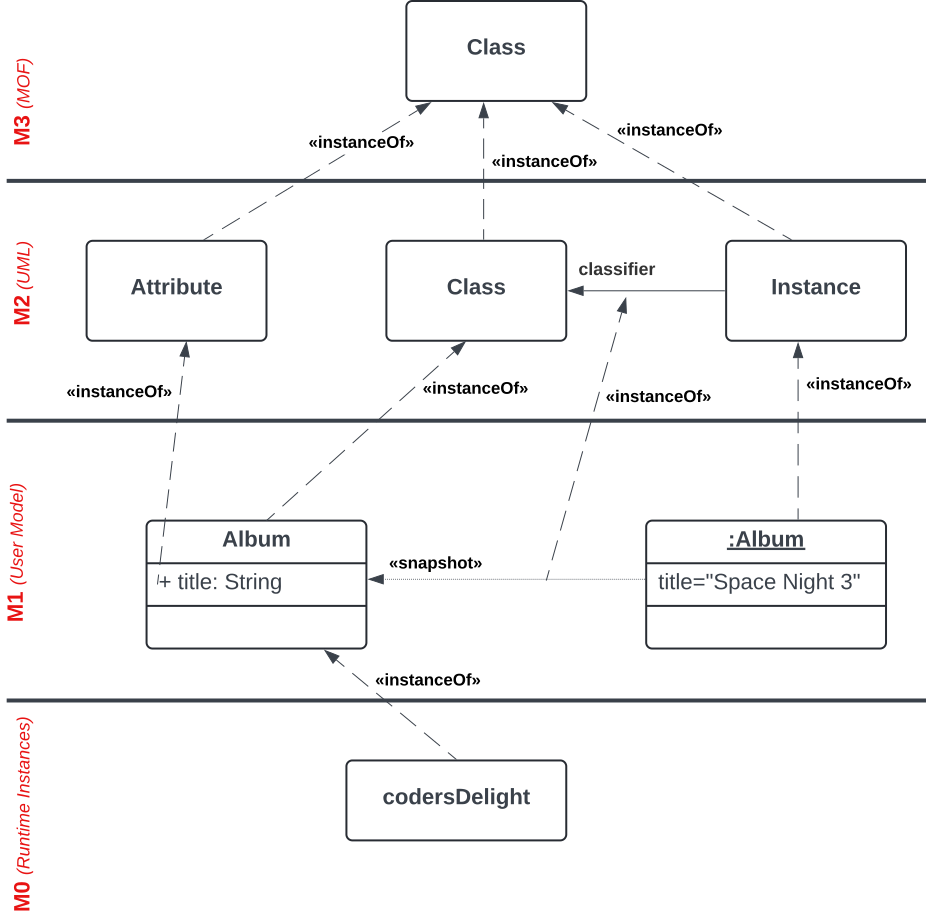
\includegraphics[scale=0.4]{part three/Einführung/img/metamodel}
    \caption{Beispiel für die verschiedenen Schichten der Metamodell Hierarchie.
        In der original Abbildung sind die Pfeilspitzen offen. (Quelle: in Anlehnung an S. 20, Figure 7.8, \url{https://www.omg.org/spec/UML/2.4.1/Infrastructure/PDF}, abgerufen 01.05.2024}
    \label{fig:metamodel-cc}
\end{figure}

\clearpage


\section{Strukturdiagramme}

\begin{tcolorbox}[title=Strukturdiagramme]
    In den \textbf{Strukturdiagrammen} werden \textbf{statische Strukturaspekte} eines Systems betrachtet.
    Für eine Systemmodellierung können alle dieser 6 Diagramme verwendet werden.

    \begin{itemize}
        \item \textbf{Klassendiagramm}: Das \textbf{Klassendiagramm} wird verwendet, um ein objektorientiertes System zu beschreiben.
        \item \textbf{Paketdiagramm}: Ein \textbf{Paketdiagramm} zeigt die Pakete eines Systems und deren Beziehungen.
        \item \textbf{Komponentendiagramm}: Stellt Komponenten oder auch \textit{Subsysteme} mit definierten Interfaces dar, um bspw. \textbf{Architekturdesign} darzustellen.
        \item \textbf{Verteilungsdiagramm}: Beschreibt eine Menge von Knoten, die die \textit{Ausführungsarchitektur} eines Systems definieren können, wobei Knoten i.d.R. \textit{Geräte} oder \textit{Softwareablaufumgebungen repräsentieren}.
        \item \textbf{Kompositionsstrukturdiagramm}: Stellt die \textbf{Komposition} von \textit{Systemstrukturen} (Klassen, Komponenten, Gesamtsystem) in einem bestimmten \textit{Kontext} mit einem bestimmten \textit{Ziel} dar (vgl. \cite[9]{Buh09}).
        \item \textbf{Objektdiagramm}: Momentaufnahme eines Systems zu genau einem \textit{Zeitpukt} während der Ausführung
    \end{itemize}

\end{tcolorbox}
\clearpage

\section{Verhaltensdiagramme}

\begin{tcolorbox}[title=Verhaltensdiagramme]
    \textbf{Verhaltensdiagramme} stellen \textit{Dynamik}, \textit{interne Abläufe} und das \textit{Zusammenspiel} der Systemteile dar, um eine Spezifikation zu vervollständigen.

    \begin{itemize}
        \item \textbf{Anwendungsfalldiagramm}: Dienen zur \textit{Spezifizierung} und \textit{Formalisierung} von \textit{Systemanforderungen}, unter Berücksichtigung von \textbf{Akteuren}, \textbf{Systemen} und \textbf{Anwendungsfällen}
        \item \textbf{Zustandsdiagramm}: Auch \textbf{Zustandsautomaten}; zeigen für ein einzelnes Objekt Zustandsänderungen während der Lebenszeit
        \item \textbf{Aktivitätsdiagramme}: Werden zur Modellierung von \textit{Kontroll}- oder \textit{Objektflüssen} oder zur Darstellung von \textit{Programmlogik} genutzt.
        \item \textbf{Interaktionsdiagramme}: Stellen das Zusammenspiel mehrerer Kommunikationspartner dar.
        Es gibt unterschiedliche Typen von Interaktionsdiagrammen, die Interaktionen auf verschiedenen \textit{Abstraktionsebenen} modellieren:
        \begin{itemize}
            \item \textbf{Sequenzdiagramm}: Zeigt den Verlauf einer Interaktion in zwei Dimensionen, \textit{Kommunikationspartner} und die Nachrichten in ihrer \textit{zeitlichen Abfolge}
            \item \textbf{Kommunikationsdiagramm}: hebt die Kommunikationsbeziehungen zwischen den Partnern hervor
            \item \textbf{Timing Diagramm}: hebt die zeitlichen Aspekte einer Interaktion hervor
            \item \textbf{Interaktionsüberblickdiagramm}: Spezialfall des \textbf{Aktivitätsdiagramms} - statt Aktionen und Aktivitäten können das \textbf{Sequenz}-, \textbf{Kommunikations}- und das \textbf{Timing}-Diagramm als Knoten verwendet werden.
        \end{itemize}
        Alle verwenden dieselben Grundelemente: \textit{Lebenslinien} der Akteure und Nachrichten, die zwischen diesen ausgetauscht werden.
    \end{itemize}
\end{tcolorbox}

\clearpage


\section{Klassendiagramm}

\begin{tcolorbox}[title=Klassendiagramm]
    Das \textbf{Klassendiagramm} beschreibt die Klassen eines Systems und die statischen Beziehungen zwischen ihnen.\\
    Sie werden in Form von Domainklassen bei der \textbf{Analyse} und als detaillierte Entwürfe von Systemklassen als \textit{Blueprint} im \textbf{gesamten Entwicklungsprozess} eingesetzt.

\end{tcolorbox}
\clearpage


\section{Assoziationsklasse (Attributierte Assoziation)}

\begin{tcolorbox}[title=Assoziationsklasse (Attributierte Assoziation)]
Eine \textbf{Assoziationsklasse} erlaubt das Hinzufügen von Operationen und Attributen zu einer Assoziation (\cite[43]{Buh09}).\\
Assoziationsklassen werden in der \textbf{Analyse} in Modellen verwendet und in dem \textbf{Entwurf} in eigenständige Klassen transformiert.\\

\noindent
Assoziationsklassen werden in der \textbf{Analyse} in Modellen verwendet und in dem \textbf{Entwurf} in eigenständige Klassen transformiert.

\blockquote[{\cite[277]{Oes05}}]{
    Eine attributierte Assoziation ist immer dann nahe liegend, wenn Attribute oder Operationen gefunden werden, die weder der einen noch der anderen Klasse zugeordnet werden können, weil sie nämlich Eigenschaften der Beziehung selbst sind.
}.\\

Bei einer attributierten Assoziation dürfen zwei beteiligte Objekte maximal nur eine Beziehung zueinander haben (vgl.~\cite[277]{Oes05})\footnote{
    \textit{Ostereich} führt dies ebenda auf Seite 278 weiter aus, in dem er beschreibt, wie eine attributierte Assoziation für ein \textit{Beschäftigtenverhältnis} zwischen \textit{Mitarbeiter} und \textit{Unternehmen} modelliert wird. Dabei wird davon ausgegangen, dass ein \textit{Mitarbeiter} nur über \textit{ein} Arbeitsverhältnis mit einem \textit{Unternehmen} in Beziehung stehen kann. Bestehen mehrere Arbeitsverhältnisse (\textit{Mitarbeiter} hat zu unterschiedlichen Zeitpunkten für das \textit{Unternehmen} gearbeitet), kann die attributierte Assoziation nicht verwendet werden.\\

\noindent
Wird eine attributierte Assoziation in eine gewöhnliche Assoziation transformiert, muss darauf geachtet werden, die Multiplizitäten richtig zu setzen (s. Abbildung~\ref{fig:assoziationsklasse}).
\end{tcolorbox}

\begin{figure}
    \centering
    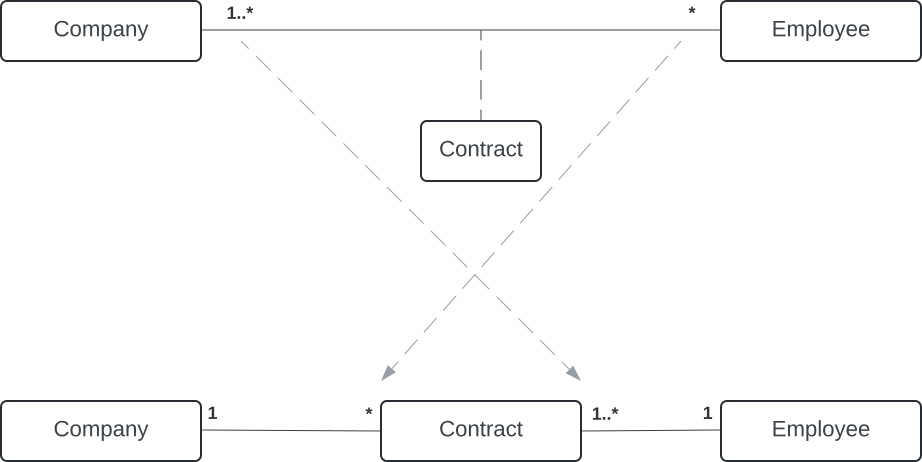
\includegraphics[scale=0.4]{part three/Klassendiagramme - Erweiterte Konzepte und Paketdiagramme/img/assoziationsklasse}
    \caption{Darstellung einer Assoziation mit Hilfe einer Assoziationsklasse (oben) sowie Transformation in gewöhnliche Assoziationen (unten). (Quelle: in Anlehnung an \cite[279, Abb. 4.4-11]{Oes05})}
    \label{fig:assoziationsklasse-cc}
\end{figure}

\clearpage


\section{Sequenzdiagramme}

\begin{tcolorbox}[title=Sequenzdiagramme]
    \textbf{Sequenzdiagramme} stellen Verhalten auf der Ebene einer Interaktion dar.\\
    In der Phase des Klassendesigns werden die Teilnehmer der Interaktionen bestimmt, weshalb Sequenzdiagramme oft in dieser Phase genutzt werden.\\
    In der \textbf{Analysephase} können Sequenzdiagramme eingesetzt werden, um die Kommunikation der bis dahin ausgemachten \textbf{Geschäftsobjekte} zu modellieren, oder um \textbf{Anwendungsfälle} weiter zu spezifizieren.
\end{tcolorbox}
\clearpage

\section{Aggregation}

\begin{tcolorbox}[title=Aggregation]
    Eine \textbf{Aggregation} ist in ihrer \semantischen Aussage unscharf (vgl.~\cite[40]{Buh09}).\\
    Sie beschreibt eine \textit{Ganzes}-\textit{Teile}-Beziehung, aber die \textit{Teile} können zu mehreren verschiedenen \textit{Ganzen} gehören.\\
    Außerdem kann ein Teil dem \textit{Ganzen} jederzeit wieder entnommen werden und das \textit{Ganze} ist nicht verantwortlich für das Erstellen der \textit{Teile}, weshalb Implementierungen beim Hinzufügen von Teilen oft schon fertige Objekte erwarten, die jeweils eines der \textit{Teile} repräsentieren.\\
    Aggregationsbeziehungen werden durch eine nicht-gefüllte Raute an der Seite der Klasse, die das Ganze repräsentiert, dargestellt.
\end{tcolorbox}
\clearpage

\section{Komposition}

\begin{tcolorbox}[title=Komposition]
    Bei einer \textbf{Komposition} handelt es sich um eine \textit{Ganzes}-\textit{Teile}-Beziehung, bei der das \textit{Ganze} verantwortlich für die Erstellung und Beseitigung der \textit{Teile} ist.
    Außerdem sind die \textit{Teile} an die \textbf{Existenz} des \textit{Ganzen} gebunden.\\
    \textit{Teile} gehören immer zu \textit{genau einem} \textit{Ganzen}.\\
    Eine Komposition wird dargestellt durch eine gefüllte Raute an der Klassenbox, die das \textit{Ganze} repräsentiert.
\end{tcolorbox}
\clearpage

\section{Paketdiagramm}

\begin{tcolorbox}[title=Komposition]
    \textbf{Paketdiagramme} zeigen Pakete und ihre Abhängigkeiten und werden in frühen Designphasen genutzt, um Strukturen (großer Systeme) aufzuzeigen.\\

    \noindent
    Elemente sollten so in Paketen gruppiert werden, dass ihr \textbf{funktionaler Zusammenhalt} (\textit{Kohäsion}, s. Abschnitt~\ref{subsec:hohe-kohasion}) klar wird.\\
    Hierdurch kann vermieden werden, dass Änderungen einer Klasse eines Paketes auch Änderungen außerhalb des Paketes erfordern.\\
    Außerdem erhöht sich die Wahrscheinlichkeit, dass einzelne Pakete als solche in anderen Projekten wiederverwendet werden können.\\

    \noindent
    In Paketdiagrammen können Beziehungen über folgende Schlüsselwörter deutlich gemacht werden:

    \begin{itemize}
        \item \guillemotleft import\guillemotright
        \item[] $\rightarrow$ \textbf{public-Import} zwischen Quell- und Zielpaket; Quellpaket kann die öffentlichen Elemente des Zielpaketes unter Verwendung des unqualifizierten und des qualifizierten Namens verwenden; die importierten Elemente sind auch für Pakete sichtbar, die das Quellpaket importieren
        \item \guillemotleft access\guillemotright
        \item[] $\rightarrow$ \textbf{privater Import} zwischen Quell- und Zielpaket; Zugriff auf Elemente des importierten Paketes ohne qualifizierenden Namen möglich; der Import eines Paketes in \textbf{Java} entspricht der \guillemotleft access\guillemotright-Beziehung
        \item \guillemotleft merge\guillemotright
        \item[] $\rightarrow$ Bei einem \textbf{merge} werden Elemente eines Zielpaketes in das Quellpaket
   \end{itemize}
\end{tcolorbox}
\clearpage

\section{Anwendungsfalldiagramm}

\begin{tcolorbox}[title=Anwendungsfalldiagramm]
    Die \textbf{Anwendungsfallanalyse} wird im Rahmen der \textbf{Anforderungsspezifikation} eingesetzt.\\

    \noindent
    Anwendungsfalldiagramme sind das am häufigsten eingesetzte Mittel zur Aufnahme und Darstellung von \textbf{Anforderungen}.\\
    Sie beschreiben selbst kein Verhalten und keine Abläufe, sondern zeigen nur die Zusammenhänge der an Anwendungsfällen beteiligten Modellelemente und sind somit ein Hilfsmittel zur Anforderungsermittlung und Verwaltung.\\

    \noindent
    Zu den wichtigsten Schritten einer Anwendungsfallanalyse gehören:
    \begin{enumerate}
        \item Akteure identifizieren
        \item Anwendungsfälle identifizieren
        \item Beschreiben der Akteure und Anwendungsfälle
        \item Identifizieren von \textit{Schlüsselobjekten}, die das System verwaltet
        \item Identifizieren der wichtigsten Anwendungsfälle (Priorisierung)
        \item detailliertere Beschreibung der Anwendungsfälle
        \item Strukturierung des Anwendungsfalldiagramms
    \end{enumerate}

    \noindent
    Anwendungsfälle beschreiben das \textbf{Szenario} der Nutzung, und nicht Features des Systems.
\end{tcolorbox}

\clearpage

\input{chapters/Anhang/CheatSheets/SE3/Aktivitätsdiagramm}
\clearpage

\section{Zustandsautomat}

\begin{tcolorbox}[title=Zustandsautomat]
    Mit \textbf{Zustandsautomaten} kann das \textit{Verhalten} von Systemen modelliert werden, wobei die \textit{Reaktionen} des Systems im Mittelpunkt stehen, und nicht die \textit{Aktionen}, wie bspw. bei den \textbf{Aktivitätsdiagrammen}.\\

    \noindent
        Ein \textbf{Zustandsautomat} kann den \textit{Lebensweg} eines Objektes modellieren, weshalb Zustandsautomaten oft im \textbf{Entwurf} als Ergänzung zu den \textbf{Klassendiagrammen} eingesetzt werden.
\end{tcolorbox}

\begin{figure}
    \centering
    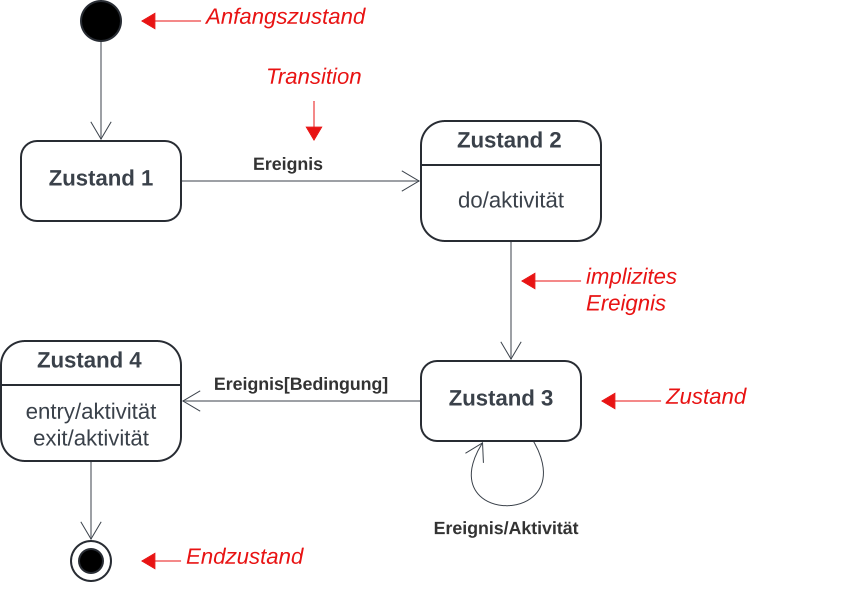
\includegraphics[scale=0.4]{part three/Zustandsautomaten/img/statechartdiagramnotation}
    \caption{Elemente eines einfachen Zustandsautomaten. Eine Transitionen wird durch ein \textbf{Ereignis} ausgelöst, das ein \textit{Signal}, ein \textit{Operationsaufruf} oder auch eine bestimmte \textit{Attributänderung} sein kann. (Quelle: in Anlehnung an \cite[90, Abb. 2.11-6]{Bal05})}
    \label{fig:statechartdiagramnotation-cc}
\end{figure}

\begin{minted}[fontsize=\small]{java}
// Beispiel für eine Implementierung eines
// Parkscheinautomaten als Zustandsautomat in Java
class Parkscheinautomat {

  // zustände
  private final int BEREIT = 0;
  private final int ZAHLUNG = 1;
  private final int ABBRUCH = 2;
  private final int BELEG   = 3;

  // Zustand; wird initial beim Starten
  // des Automaten gesetzt
  private int zustand;

  // Methoden lösen Aktionen beim Eintritt
  // in die jeweiligen Zustände aus
  private int zahlung() {
    // verarbeiten
    // danach neuen Zustand zurückliefern...
    ...
    return BEREIT;
  }

   ...

  private void bereit() {
    while (true) {
      // eingabe überprüfen und
      // ggf. Zustandswechsel auslösen:
      // Zustand als Attribut setzen
      ...
    }
  }

  public void start() {
    zustand = BEREIT;

    while(true) {
      switch (zustand) {
        case BEREIT:
          zustand = bereit();
        // ... weiteres Verhalten
        ...
      }
    }
  }
}
\end{minted}
\clearpage

	\part{Teil 3 - Systemmodellierung}

\newpage
\section*{Lernziele Teil 3}

\begin{itemize}
    \item den Sprachaufbau der UML 2.0 und die wesentlichen und wichtigsten Modellierungskonzepte und Diagramme beherrschen
    \item die Fähigkeit besitzen, UML 2.0 Modelle zu entwickeln
    \item in der Lage sein, UML 2.0 Modelle in der Programmiersprache Java auszudrücken
\end{itemize}

\newpage
	

\section{Inhalt SE3}

\section*{1. Übersicht UML}

\subsection*{Lernziele}
\begin{itemize}
    \item einen Einblick in den Sprachaufbau der UML 2.0 gewinnen
    \item einen Überblick über die Diagramme der UML 2.0 und deren Zweck haben
\end{itemize}

\subsection*{Zusammenfassung}
\begin{itemize}
    \item Die \textbf{UML} ist eine weit verbreitete Modellierungssprache zur Modellierung objektorientierter Softwaresysteme.
    \item Die UML 2.0 Spezifikation besteht aus vier Teilen:
    \begin{enumerate}
        \item \textbf{Superstructure}: Diagrammtypen
        \item \textbf{Infrastructure}: Modellierungskonzepte
        \item \textbf{OCL}: formale Sprache zur Formulierung von Einschränkungen
        \item \textbf{Diagram Interchange}: Austauschformate
    \end{enumerate}
    \item Die UML kann im \textbf{Sketching} oder \textbf{Blueprint Modus} eingesetzt werden, oder als Grundlage für \textbf{automatische Codegenerierung}
    \item Die UML ist an keinen speziellen Entwicklungsprozess gebunden
\end{itemize}

\section*{2. Klassendiagramme}

\subsection*{Lernziele}
\begin{itemize}
    \item wissen, wie Klassendiagramme im Entwicklungsprozess eingesetzt werden
    \item Klassendiagramme für Analyse- und Designentscheidungen einsetzen können
    \item die wichtigsten Modellierungskonzepte kennen
    \item sinnvolle Klassendiagramme erstellen und Java-Implementierungen ableiten können
    \item Klassendiagramme aus Java Quellcode erzeugen können
\end{itemize}

\subsection*{Zusammenfassung}

\begin{itemize}
    \item \textbf{Klassendiagramme} dienen zur \textbf{strukturellen Darstellung} von Softwaresystemen
    \item hierbei werden Klassen und \textbf{Beziehungen} zwischen Klassen dargestellt
    \item Properties können durch die \textbf{Attribut}- oder \textbf{Assoziationsnotation} modelliert werden
    \item Operationen werden als separate Zeile in ihrem Compartment dargestellt
    \item im Klassendiagramm können auch \textbf{Generalisierungsbeziehungen} modelliert werden
    \item \textbf{Abhängigkeitsbeziehungen} drücken ein Verhältnis zwischen \textbf{Client} und \textbf{Supplier} aus
\end{itemize}

\section*{3. Objektorientierter Entwurf}

\subsection*{Lernziele}
\begin{itemize}
    \item das Wesen einer Interaktion kennen
    \item wissen, wie Sequenzdiagramme im Entwicklungsprozess eingesetzt werden
    \item Sequenzdiagramme für Analyse- und Designentscheidungen sowie zur Darstellung von Kontrollflüssen einsetzen können
    \item die wichtigsten Modellierungskonzepte kennen
    \item sinnvolle Sequenzdiagramme erstellen und Java-Implementierungen ableiten können
    \item Sequenzdiagramme aus Java Quellcode erzeugen können
\end{itemize}

\subsection*{Zusammenfassung}

\begin{itemize}
    \item Sequenzdiagramme sind \textbf{Verhaltensdiagramme}
    und können im gesamten Entwicklungszyklus zur Modellierung von Interaktionen angewendet werden
    \item Interaktionen bestehen im Wesentlichen aus dem Nachrichtenaustausch zwischen verschiedenen Kommunikationspartnern
    \item in den meisten Fällen wird die Kommunikation von Objekten von Klassen modelliert, aber es können auch Teilnehmer auf anderen Ebenen modelliert werden
    \item gewöhnlich gibt ein Sequenzdiagramm einen \textbf{Anwendungsfall} (\textit{Szenario}) wieder
    \item sie dienen nicht dazu, um Zustandsänderungen darzustellen (hierfür werden Zustandsdiagramme verwendet)
    \item Sequenzdiagramme sind \textit{nicht} gut geeignet für die Darstellung von
    \begin{itemize}
        \item nebenläufigem Verhalten (\textit{asynchrone} Nachrichten, \textit{kombiniertes Fragment})
        \item Schleifen und alternativem Verhalten (\textit{kombinierte Fragmente})
        \item[] $\rightarrow$  für beide Fälle sind \textbf{Aktivitätsdiagramme} besser geeignet
    \end{itemize}
\end{itemize}

\section*{4. Klassendiagramme - Erweiterte Konzepte und Paketdiagramme}

\subsection*{Lernziele}
\begin{itemize}
    \item erweiterte Modellierungskonzepte in Klassendiagrammen für den Detailentwurf von Systemen kennen
    \item die Konsequenzen dieser Konzepte in der Implementierung kennen
    \item wissen, wie Paketdiagramme im Entwicklungsprozess eingesetzt werden
    \item die Modellierungskonzepte in Paketdiagrammen kennen
    \item anhand von Paketdiagrammen Software-Architekturen gestalten und bewerten können
\end{itemize}

\subsection*{Zusammenfassung}

\begin{itemize}
    \item Die vorgestellten erweiterten Konzepte werden vor allem im \textbf{Feinentwurf} von Klassenstrukturen eingesetzt.
    \item Generell gilt, dass die Spezifikationen von Objekten und Properties nur so detailliert ausgeführt werden sollen, wie nötig: Sind Details für das Verständnis unnötig, sollte darauf verzichtet werden.
    \item \textbf{Generalisierungsbeziehungen} sollten grundsätzlich modelliert werden.
    \item Ist eine \textbf{Komposition} statt einer Generalisierung für den Sachverhalt möglich, sollte diese verwendet werden: ``Favor object composition over inheritance.`` (\cite[19 f.]{GHJV94})
    \item \textbf{Kompositionsbeziehungen} geben eindeutige Impulse für eine Implementierung, \textbf{Aggregationsbeziehungen} sind in ihrer semantischen Aussage nicht sehr eindeutig
    \item \textbf{Assoziationsklassen} sind in ihrer frühen Designphase empfehlenswert, die Realisierung (mit {bspw.} Java) erfordert aber eine Transformation in eine volle Klasse, wobei die Multiplizitäten angepasst werden müssen
    \item Elemente können in \textbf{Paketen} zusamengefasst und unter einem gemeinsamen Namensraum gruppiert werden
\end{itemize}

\section*{4. Anwendungsfalldiagramm (Use-Case-Diagramm)}

\subsection*{Lernziele}
\begin{itemize}
    \item wissen, wie die Anwendungsfallanalyse im Rahmen der Anforderungsspezifikation eingesetzt wird
    \item Prozessschritte der Anwendungsfallanalyse beherrschen
    \item die wichtigsten Modellierungskonzepte in Anwendungsfalldiagrammen kennen
    \item den Aufbau einer Anwendungsfallbeschreibung kennen
\end{itemize}

\subsection*{Zusammenfassung}

\begin{itemize}
    \item \textbf{Anwendungsfalldiagramme} besitzen eine einfache Notation, um \textbf{Akteure} und \textbf{Anwendungsfälle} eines \textbf{Systems} grafisch darzustellen
    \item auf Basis eines Anwendungsfalldiagramms lässt sich ermitteln, ob die Anwendungsfälle gewünschtes Verhalten realisieren bzw. Beziehungen zu einem oder mehreren Akteuren haben
    \item Anwendungsfälle und Akteure \textit{müssen} zusätzlich textlich beschrieben werden
\end{itemize}

\section*{5. Aktivitätsdiagramme}

\subsection*{Lernziele}
\begin{itemize}
    \item wissen, wie Aktivitätsdiagramme im Rahmen der Verhaltensanalyse in verschiedenen Prozessphasen eingesetzt werden können
    \item die wichtigsten Modellierungskonzepte in Aktivitätsdiagrammen kennen
    \item Aktivitätsdiagramme interpretieren, erstellen und implementieren können
\end{itemize}

\subsection*{Zusammenfassung}

\begin{itemize}
    \item \textbf{Aktivitätsdiagramme} gehören zu den \textbf{Verhaltensdiagrammen} und können im \textit{gesamten} \textbf{Entwicklungsprozess} eingesetzt werden
    \item durch ein Aktivitätsdiagramm kann gezeigt werden, wie \textbf{Verhalten} realisiert wird
    \item es können mehrere \textbf{Aktivitäten} dargestellt werden
    \item \textbf{Aktivitätskanten} und \textbf{Aktivitätsknoten} werden zur Beschreibung von Verhalten verwendet
\end{itemize}

\section*{5. Zustandsautomaten}

\subsection*{Lernziele}
\begin{itemize}
    \item wissen, wie Zustandsdiagramme im Rahmen der Verhaltensanalyse einzelner Objekte eingesetzt werden können
    \item die wichtigsten Modellierungskonzepte in Zustandsdiagrammen kennen
    \item Zustandsdiagramme interpretieren, erstellen und implementieren können
\end{itemize}

\subsection*{Zusammenfassung}

\begin{itemize}
    \item Das \textbf{Zustandsdiagramm} gehört wie das \textbf{Aktivitätsdiagramm} zu den \textbf{Verhaltensdiagrammen}.
    \item Ein Zustandsdiagramm zeigt den \textbf{Lebensweg} eines \textbf{Objektes}.
    \item \textbf{Attributwerte} bestimmen den Zustand eines Objektes.
    \item \textbf{Transitionen} zwischen Zuständen werden durch \textbf{Guards} und \textbf{Events} gesteuert.
    \item Während der Transitionen können \textbf{Effekte} (\textit{Aktivitäten}) realisiert werden.
    \item Die Modellierung \textbf{zusammengesetzter Zustände} ist ebenfalls möglich.
    \item Für die Darstellung \textbf{paralleler} oder  \textbf{konkurrierender} Abläufe können \textbf{Regionen} modelliert werden.
\end{itemize}
\clearpage


\section{UML Modellierung}

\begin{tcolorbox}[title=UML Modellierung]
    \textbf{Modelle} haben die Aufgabe, den Bezug zum Original (Programm, Softwaresystem) herzustellen, sowie zu der \textit{Anwendungsumgebung}.\\
    Ein \textbf{Modell} enthält alle \textbf{Modellelemente}, die zur Beschreibung eines Softwaresystems nötig sind.\\

    \noindent
    Ein \textbf{Modellelement} wird als Element in einem UML Modell von einem Benutzer erstellt und auf verschiedenen \textbf{Diagrammen} (Struktur-/Verhaltensdiagrammen) platziert, und wird durch die \textbf{UML Modellierungskonzepte} als Metaklasse des \textbf{Metamodells} der UML beschrieben: \textbf{Modellelemente} werden aus Modellierungskonzepten instanziiert.\\

    \noindent
       Das \textbf{UML Metamodell} regelt, in welchem Zusammenhang \textbf{UML Modellierungskonzepte} in Modellen auftreten dürfen, und welche Eigenschaften und Beziehungen zu anderen Sprachelementen zulässig sind.\\

       \noindent
       Die im \textbf{Metamodell} verwendeten Erklärungen basieren auf einer abstrakten Syntax, für deren Beschreibung eine Untermenge (\textit{Klassendiagramme}) der UML verwendet wird.\\
        Die \textbf{Semantik} der Modellierungskonzepte wird textlich beschrieben, zur Formalisierung von Regeln für die syntaktische Korrektheit wird die \textbf{OCL} (\textit{Object Constraint Language}) verwendet.
\end{tcolorbox}

\begin{figure}
    \centering
    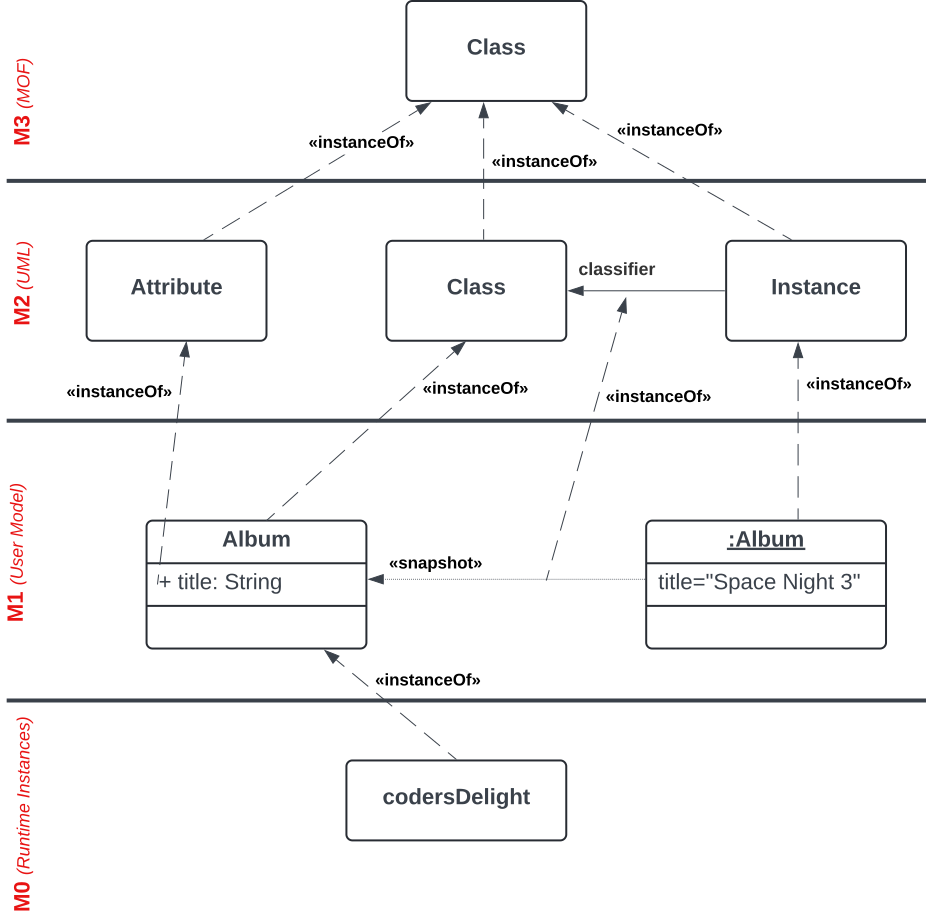
\includegraphics[scale=0.4]{part three/Einführung/img/metamodel}
    \caption{Beispiel für die verschiedenen Schichten der Metamodell Hierarchie.
        In der original Abbildung sind die Pfeilspitzen offen. (Quelle: in Anlehnung an S. 20, Figure 7.8, \url{https://www.omg.org/spec/UML/2.4.1/Infrastructure/PDF}, abgerufen 01.05.2024}
    \label{fig:metamodel-cc}
\end{figure}

\clearpage


\section{Strukturdiagramme}

\begin{tcolorbox}[title=Strukturdiagramme]
    In den \textbf{Strukturdiagrammen} werden \textbf{statische Strukturaspekte} eines Systems betrachtet.
    Für eine Systemmodellierung können alle dieser 6 Diagramme verwendet werden.

    \begin{itemize}
        \item \textbf{Klassendiagramm}: Das \textbf{Klassendiagramm} wird verwendet, um ein objektorientiertes System zu beschreiben.
        \item \textbf{Paketdiagramm}: Ein \textbf{Paketdiagramm} zeigt die Pakete eines Systems und deren Beziehungen.
        \item \textbf{Komponentendiagramm}: Stellt Komponenten oder auch \textit{Subsysteme} mit definierten Interfaces dar, um bspw. \textbf{Architekturdesign} darzustellen.
        \item \textbf{Verteilungsdiagramm}: Beschreibt eine Menge von Knoten, die die \textit{Ausführungsarchitektur} eines Systems definieren können, wobei Knoten i.d.R. \textit{Geräte} oder \textit{Softwareablaufumgebungen repräsentieren}.
        \item \textbf{Kompositionsstrukturdiagramm}: Stellt die \textbf{Komposition} von \textit{Systemstrukturen} (Klassen, Komponenten, Gesamtsystem) in einem bestimmten \textit{Kontext} mit einem bestimmten \textit{Ziel} dar (vgl. \cite[9]{Buh09}).
        \item \textbf{Objektdiagramm}: Momentaufnahme eines Systems zu genau einem \textit{Zeitpukt} während der Ausführung
    \end{itemize}

\end{tcolorbox}
\clearpage

\section{Verhaltensdiagramme}

\begin{tcolorbox}[title=Verhaltensdiagramme]
    \textbf{Verhaltensdiagramme} stellen \textit{Dynamik}, \textit{interne Abläufe} und das \textit{Zusammenspiel} der Systemteile dar, um eine Spezifikation zu vervollständigen.

    \begin{itemize}
        \item \textbf{Anwendungsfalldiagramm}: Dienen zur \textit{Spezifizierung} und \textit{Formalisierung} von \textit{Systemanforderungen}, unter Berücksichtigung von \textbf{Akteuren}, \textbf{Systemen} und \textbf{Anwendungsfällen}
        \item \textbf{Zustandsdiagramm}: Auch \textbf{Zustandsautomaten}; zeigen für ein einzelnes Objekt Zustandsänderungen während der Lebenszeit
        \item \textbf{Aktivitätsdiagramme}: Werden zur Modellierung von \textit{Kontroll}- oder \textit{Objektflüssen} oder zur Darstellung von \textit{Programmlogik} genutzt.
        \item \textbf{Interaktionsdiagramme}: Stellen das Zusammenspiel mehrerer Kommunikationspartner dar.
        Es gibt unterschiedliche Typen von Interaktionsdiagrammen, die Interaktionen auf verschiedenen \textit{Abstraktionsebenen} modellieren:
        \begin{itemize}
            \item \textbf{Sequenzdiagramm}: Zeigt den Verlauf einer Interaktion in zwei Dimensionen, \textit{Kommunikationspartner} und die Nachrichten in ihrer \textit{zeitlichen Abfolge}
            \item \textbf{Kommunikationsdiagramm}: hebt die Kommunikationsbeziehungen zwischen den Partnern hervor
            \item \textbf{Timing Diagramm}: hebt die zeitlichen Aspekte einer Interaktion hervor
            \item \textbf{Interaktionsüberblickdiagramm}: Spezialfall des \textbf{Aktivitätsdiagramms} - statt Aktionen und Aktivitäten können das \textbf{Sequenz}-, \textbf{Kommunikations}- und das \textbf{Timing}-Diagramm als Knoten verwendet werden.
        \end{itemize}
        Alle verwenden dieselben Grundelemente: \textit{Lebenslinien} der Akteure und Nachrichten, die zwischen diesen ausgetauscht werden.
    \end{itemize}
\end{tcolorbox}

\clearpage


\section{Klassendiagramm}

\begin{tcolorbox}[title=Klassendiagramm]
    Das \textbf{Klassendiagramm} beschreibt die Klassen eines Systems und die statischen Beziehungen zwischen ihnen.\\
    Sie werden in Form von Domainklassen bei der \textbf{Analyse} und als detaillierte Entwürfe von Systemklassen als \textit{Blueprint} im \textbf{gesamten Entwicklungsprozess} eingesetzt.

\end{tcolorbox}
\clearpage


\section{Assoziationsklasse (Attributierte Assoziation)}

\begin{tcolorbox}[title=Assoziationsklasse (Attributierte Assoziation)]
Eine \textbf{Assoziationsklasse} erlaubt das Hinzufügen von Operationen und Attributen zu einer Assoziation (\cite[43]{Buh09}).\\
Assoziationsklassen werden in der \textbf{Analyse} in Modellen verwendet und in dem \textbf{Entwurf} in eigenständige Klassen transformiert.\\

\noindent
Assoziationsklassen werden in der \textbf{Analyse} in Modellen verwendet und in dem \textbf{Entwurf} in eigenständige Klassen transformiert.

\blockquote[{\cite[277]{Oes05}}]{
    Eine attributierte Assoziation ist immer dann nahe liegend, wenn Attribute oder Operationen gefunden werden, die weder der einen noch der anderen Klasse zugeordnet werden können, weil sie nämlich Eigenschaften der Beziehung selbst sind.
}.\\

Bei einer attributierten Assoziation dürfen zwei beteiligte Objekte maximal nur eine Beziehung zueinander haben (vgl.~\cite[277]{Oes05})\footnote{
    \textit{Ostereich} führt dies ebenda auf Seite 278 weiter aus, in dem er beschreibt, wie eine attributierte Assoziation für ein \textit{Beschäftigtenverhältnis} zwischen \textit{Mitarbeiter} und \textit{Unternehmen} modelliert wird. Dabei wird davon ausgegangen, dass ein \textit{Mitarbeiter} nur über \textit{ein} Arbeitsverhältnis mit einem \textit{Unternehmen} in Beziehung stehen kann. Bestehen mehrere Arbeitsverhältnisse (\textit{Mitarbeiter} hat zu unterschiedlichen Zeitpunkten für das \textit{Unternehmen} gearbeitet), kann die attributierte Assoziation nicht verwendet werden.\\

\noindent
Wird eine attributierte Assoziation in eine gewöhnliche Assoziation transformiert, muss darauf geachtet werden, die Multiplizitäten richtig zu setzen (s. Abbildung~\ref{fig:assoziationsklasse}).
\end{tcolorbox}

\begin{figure}
    \centering
    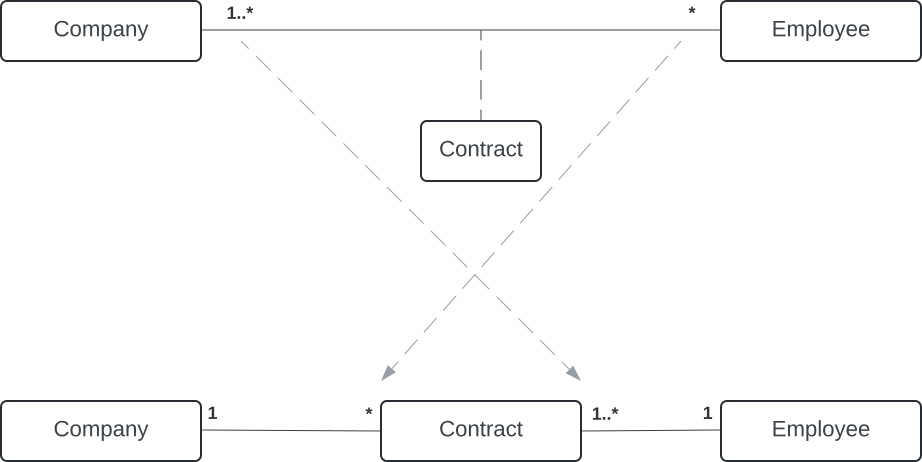
\includegraphics[scale=0.4]{part three/Klassendiagramme - Erweiterte Konzepte und Paketdiagramme/img/assoziationsklasse}
    \caption{Darstellung einer Assoziation mit Hilfe einer Assoziationsklasse (oben) sowie Transformation in gewöhnliche Assoziationen (unten). (Quelle: in Anlehnung an \cite[279, Abb. 4.4-11]{Oes05})}
    \label{fig:assoziationsklasse-cc}
\end{figure}

\clearpage


\section{Sequenzdiagramme}

\begin{tcolorbox}[title=Sequenzdiagramme]
    \textbf{Sequenzdiagramme} stellen Verhalten auf der Ebene einer Interaktion dar.\\
    In der Phase des Klassendesigns werden die Teilnehmer der Interaktionen bestimmt, weshalb Sequenzdiagramme oft in dieser Phase genutzt werden.\\
    In der \textbf{Analysephase} können Sequenzdiagramme eingesetzt werden, um die Kommunikation der bis dahin ausgemachten \textbf{Geschäftsobjekte} zu modellieren, oder um \textbf{Anwendungsfälle} weiter zu spezifizieren.
\end{tcolorbox}
\clearpage

\section{Aggregation}

\begin{tcolorbox}[title=Aggregation]
    Eine \textbf{Aggregation} ist in ihrer \semantischen Aussage unscharf (vgl.~\cite[40]{Buh09}).\\
    Sie beschreibt eine \textit{Ganzes}-\textit{Teile}-Beziehung, aber die \textit{Teile} können zu mehreren verschiedenen \textit{Ganzen} gehören.\\
    Außerdem kann ein Teil dem \textit{Ganzen} jederzeit wieder entnommen werden und das \textit{Ganze} ist nicht verantwortlich für das Erstellen der \textit{Teile}, weshalb Implementierungen beim Hinzufügen von Teilen oft schon fertige Objekte erwarten, die jeweils eines der \textit{Teile} repräsentieren.\\
    Aggregationsbeziehungen werden durch eine nicht-gefüllte Raute an der Seite der Klasse, die das Ganze repräsentiert, dargestellt.
\end{tcolorbox}
\clearpage

\section{Komposition}

\begin{tcolorbox}[title=Komposition]
    Bei einer \textbf{Komposition} handelt es sich um eine \textit{Ganzes}-\textit{Teile}-Beziehung, bei der das \textit{Ganze} verantwortlich für die Erstellung und Beseitigung der \textit{Teile} ist.
    Außerdem sind die \textit{Teile} an die \textbf{Existenz} des \textit{Ganzen} gebunden.\\
    \textit{Teile} gehören immer zu \textit{genau einem} \textit{Ganzen}.\\
    Eine Komposition wird dargestellt durch eine gefüllte Raute an der Klassenbox, die das \textit{Ganze} repräsentiert.
\end{tcolorbox}
\clearpage

\section{Paketdiagramm}

\begin{tcolorbox}[title=Komposition]
    \textbf{Paketdiagramme} zeigen Pakete und ihre Abhängigkeiten und werden in frühen Designphasen genutzt, um Strukturen (großer Systeme) aufzuzeigen.\\

    \noindent
    Elemente sollten so in Paketen gruppiert werden, dass ihr \textbf{funktionaler Zusammenhalt} (\textit{Kohäsion}, s. Abschnitt~\ref{subsec:hohe-kohasion}) klar wird.\\
    Hierdurch kann vermieden werden, dass Änderungen einer Klasse eines Paketes auch Änderungen außerhalb des Paketes erfordern.\\
    Außerdem erhöht sich die Wahrscheinlichkeit, dass einzelne Pakete als solche in anderen Projekten wiederverwendet werden können.\\

    \noindent
    In Paketdiagrammen können Beziehungen über folgende Schlüsselwörter deutlich gemacht werden:

    \begin{itemize}
        \item \guillemotleft import\guillemotright
        \item[] $\rightarrow$ \textbf{public-Import} zwischen Quell- und Zielpaket; Quellpaket kann die öffentlichen Elemente des Zielpaketes unter Verwendung des unqualifizierten und des qualifizierten Namens verwenden; die importierten Elemente sind auch für Pakete sichtbar, die das Quellpaket importieren
        \item \guillemotleft access\guillemotright
        \item[] $\rightarrow$ \textbf{privater Import} zwischen Quell- und Zielpaket; Zugriff auf Elemente des importierten Paketes ohne qualifizierenden Namen möglich; der Import eines Paketes in \textbf{Java} entspricht der \guillemotleft access\guillemotright-Beziehung
        \item \guillemotleft merge\guillemotright
        \item[] $\rightarrow$ Bei einem \textbf{merge} werden Elemente eines Zielpaketes in das Quellpaket
   \end{itemize}
\end{tcolorbox}
\clearpage

\section{Anwendungsfalldiagramm}

\begin{tcolorbox}[title=Anwendungsfalldiagramm]
    Die \textbf{Anwendungsfallanalyse} wird im Rahmen der \textbf{Anforderungsspezifikation} eingesetzt.\\

    \noindent
    Anwendungsfalldiagramme sind das am häufigsten eingesetzte Mittel zur Aufnahme und Darstellung von \textbf{Anforderungen}.\\
    Sie beschreiben selbst kein Verhalten und keine Abläufe, sondern zeigen nur die Zusammenhänge der an Anwendungsfällen beteiligten Modellelemente und sind somit ein Hilfsmittel zur Anforderungsermittlung und Verwaltung.\\

    \noindent
    Zu den wichtigsten Schritten einer Anwendungsfallanalyse gehören:
    \begin{enumerate}
        \item Akteure identifizieren
        \item Anwendungsfälle identifizieren
        \item Beschreiben der Akteure und Anwendungsfälle
        \item Identifizieren von \textit{Schlüsselobjekten}, die das System verwaltet
        \item Identifizieren der wichtigsten Anwendungsfälle (Priorisierung)
        \item detailliertere Beschreibung der Anwendungsfälle
        \item Strukturierung des Anwendungsfalldiagramms
    \end{enumerate}

    \noindent
    Anwendungsfälle beschreiben das \textbf{Szenario} der Nutzung, und nicht Features des Systems.
\end{tcolorbox}

\clearpage

\input{chapters/Anhang/CheatSheets/SE3/Aktivitätsdiagramm}
\clearpage

\section{Zustandsautomat}

\begin{tcolorbox}[title=Zustandsautomat]
    Mit \textbf{Zustandsautomaten} kann das \textit{Verhalten} von Systemen modelliert werden, wobei die \textit{Reaktionen} des Systems im Mittelpunkt stehen, und nicht die \textit{Aktionen}, wie bspw. bei den \textbf{Aktivitätsdiagrammen}.\\

    \noindent
        Ein \textbf{Zustandsautomat} kann den \textit{Lebensweg} eines Objektes modellieren, weshalb Zustandsautomaten oft im \textbf{Entwurf} als Ergänzung zu den \textbf{Klassendiagrammen} eingesetzt werden.
\end{tcolorbox}

\begin{figure}
    \centering
    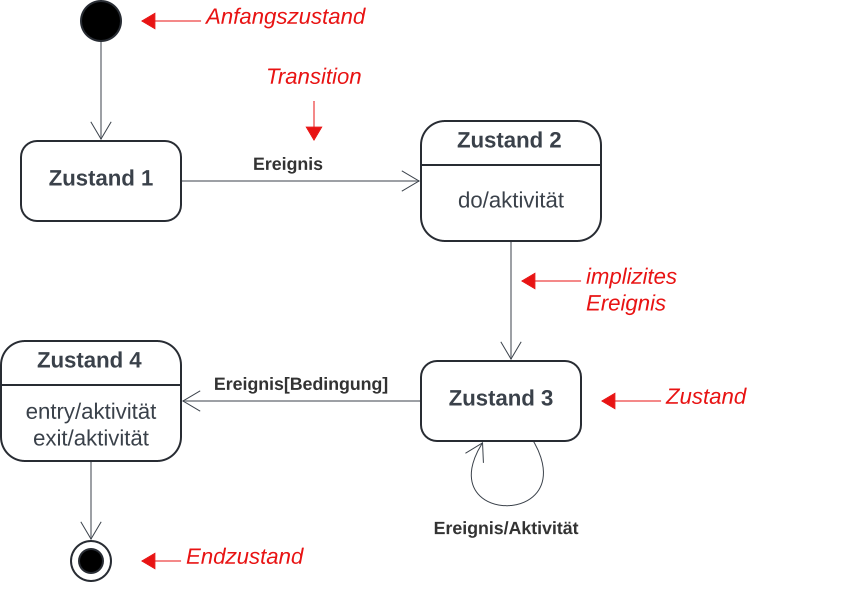
\includegraphics[scale=0.4]{part three/Zustandsautomaten/img/statechartdiagramnotation}
    \caption{Elemente eines einfachen Zustandsautomaten. Eine Transitionen wird durch ein \textbf{Ereignis} ausgelöst, das ein \textit{Signal}, ein \textit{Operationsaufruf} oder auch eine bestimmte \textit{Attributänderung} sein kann. (Quelle: in Anlehnung an \cite[90, Abb. 2.11-6]{Bal05})}
    \label{fig:statechartdiagramnotation-cc}
\end{figure}

\begin{minted}[fontsize=\small]{java}
// Beispiel für eine Implementierung eines
// Parkscheinautomaten als Zustandsautomat in Java
class Parkscheinautomat {

  // zustände
  private final int BEREIT = 0;
  private final int ZAHLUNG = 1;
  private final int ABBRUCH = 2;
  private final int BELEG   = 3;

  // Zustand; wird initial beim Starten
  // des Automaten gesetzt
  private int zustand;

  // Methoden lösen Aktionen beim Eintritt
  // in die jeweiligen Zustände aus
  private int zahlung() {
    // verarbeiten
    // danach neuen Zustand zurückliefern...
    ...
    return BEREIT;
  }

   ...

  private void bereit() {
    while (true) {
      // eingabe überprüfen und
      // ggf. Zustandswechsel auslösen:
      // Zustand als Attribut setzen
      ...
    }
  }

  public void start() {
    zustand = BEREIT;

    while(true) {
      switch (zustand) {
        case BEREIT:
          zustand = bereit();
        // ... weiteres Verhalten
        ...
      }
    }
  }
}
\end{minted}
\clearpage
	

\section{Inhalt SE3}

\section*{1. Übersicht UML}

\subsection*{Lernziele}
\begin{itemize}
    \item einen Einblick in den Sprachaufbau der UML 2.0 gewinnen
    \item einen Überblick über die Diagramme der UML 2.0 und deren Zweck haben
\end{itemize}

\subsection*{Zusammenfassung}
\begin{itemize}
    \item Die \textbf{UML} ist eine weit verbreitete Modellierungssprache zur Modellierung objektorientierter Softwaresysteme.
    \item Die UML 2.0 Spezifikation besteht aus vier Teilen:
    \begin{enumerate}
        \item \textbf{Superstructure}: Diagrammtypen
        \item \textbf{Infrastructure}: Modellierungskonzepte
        \item \textbf{OCL}: formale Sprache zur Formulierung von Einschränkungen
        \item \textbf{Diagram Interchange}: Austauschformate
    \end{enumerate}
    \item Die UML kann im \textbf{Sketching} oder \textbf{Blueprint Modus} eingesetzt werden, oder als Grundlage für \textbf{automatische Codegenerierung}
    \item Die UML ist an keinen speziellen Entwicklungsprozess gebunden
\end{itemize}

\section*{2. Klassendiagramme}

\subsection*{Lernziele}
\begin{itemize}
    \item wissen, wie Klassendiagramme im Entwicklungsprozess eingesetzt werden
    \item Klassendiagramme für Analyse- und Designentscheidungen einsetzen können
    \item die wichtigsten Modellierungskonzepte kennen
    \item sinnvolle Klassendiagramme erstellen und Java-Implementierungen ableiten können
    \item Klassendiagramme aus Java Quellcode erzeugen können
\end{itemize}

\subsection*{Zusammenfassung}

\begin{itemize}
    \item \textbf{Klassendiagramme} dienen zur \textbf{strukturellen Darstellung} von Softwaresystemen
    \item hierbei werden Klassen und \textbf{Beziehungen} zwischen Klassen dargestellt
    \item Properties können durch die \textbf{Attribut}- oder \textbf{Assoziationsnotation} modelliert werden
    \item Operationen werden als separate Zeile in ihrem Compartment dargestellt
    \item im Klassendiagramm können auch \textbf{Generalisierungsbeziehungen} modelliert werden
    \item \textbf{Abhängigkeitsbeziehungen} drücken ein Verhältnis zwischen \textbf{Client} und \textbf{Supplier} aus
\end{itemize}

\section*{3. Objektorientierter Entwurf}

\subsection*{Lernziele}
\begin{itemize}
    \item das Wesen einer Interaktion kennen
    \item wissen, wie Sequenzdiagramme im Entwicklungsprozess eingesetzt werden
    \item Sequenzdiagramme für Analyse- und Designentscheidungen sowie zur Darstellung von Kontrollflüssen einsetzen können
    \item die wichtigsten Modellierungskonzepte kennen
    \item sinnvolle Sequenzdiagramme erstellen und Java-Implementierungen ableiten können
    \item Sequenzdiagramme aus Java Quellcode erzeugen können
\end{itemize}

\subsection*{Zusammenfassung}

\begin{itemize}
    \item Sequenzdiagramme sind \textbf{Verhaltensdiagramme}
    und können im gesamten Entwicklungszyklus zur Modellierung von Interaktionen angewendet werden
    \item Interaktionen bestehen im Wesentlichen aus dem Nachrichtenaustausch zwischen verschiedenen Kommunikationspartnern
    \item in den meisten Fällen wird die Kommunikation von Objekten von Klassen modelliert, aber es können auch Teilnehmer auf anderen Ebenen modelliert werden
    \item gewöhnlich gibt ein Sequenzdiagramm einen \textbf{Anwendungsfall} (\textit{Szenario}) wieder
    \item sie dienen nicht dazu, um Zustandsänderungen darzustellen (hierfür werden Zustandsdiagramme verwendet)
    \item Sequenzdiagramme sind \textit{nicht} gut geeignet für die Darstellung von
    \begin{itemize}
        \item nebenläufigem Verhalten (\textit{asynchrone} Nachrichten, \textit{kombiniertes Fragment})
        \item Schleifen und alternativem Verhalten (\textit{kombinierte Fragmente})
        \item[] $\rightarrow$  für beide Fälle sind \textbf{Aktivitätsdiagramme} besser geeignet
    \end{itemize}
\end{itemize}

\section*{4. Klassendiagramme - Erweiterte Konzepte und Paketdiagramme}

\subsection*{Lernziele}
\begin{itemize}
    \item erweiterte Modellierungskonzepte in Klassendiagrammen für den Detailentwurf von Systemen kennen
    \item die Konsequenzen dieser Konzepte in der Implementierung kennen
    \item wissen, wie Paketdiagramme im Entwicklungsprozess eingesetzt werden
    \item die Modellierungskonzepte in Paketdiagrammen kennen
    \item anhand von Paketdiagrammen Software-Architekturen gestalten und bewerten können
\end{itemize}

\subsection*{Zusammenfassung}

\begin{itemize}
    \item Die vorgestellten erweiterten Konzepte werden vor allem im \textbf{Feinentwurf} von Klassenstrukturen eingesetzt.
    \item Generell gilt, dass die Spezifikationen von Objekten und Properties nur so detailliert ausgeführt werden sollen, wie nötig: Sind Details für das Verständnis unnötig, sollte darauf verzichtet werden.
    \item \textbf{Generalisierungsbeziehungen} sollten grundsätzlich modelliert werden.
    \item Ist eine \textbf{Komposition} statt einer Generalisierung für den Sachverhalt möglich, sollte diese verwendet werden: ``Favor object composition over inheritance.`` (\cite[19 f.]{GHJV94})
    \item \textbf{Kompositionsbeziehungen} geben eindeutige Impulse für eine Implementierung, \textbf{Aggregationsbeziehungen} sind in ihrer semantischen Aussage nicht sehr eindeutig
    \item \textbf{Assoziationsklassen} sind in ihrer frühen Designphase empfehlenswert, die Realisierung (mit {bspw.} Java) erfordert aber eine Transformation in eine volle Klasse, wobei die Multiplizitäten angepasst werden müssen
    \item Elemente können in \textbf{Paketen} zusamengefasst und unter einem gemeinsamen Namensraum gruppiert werden
\end{itemize}

\section*{4. Anwendungsfalldiagramm (Use-Case-Diagramm)}

\subsection*{Lernziele}
\begin{itemize}
    \item wissen, wie die Anwendungsfallanalyse im Rahmen der Anforderungsspezifikation eingesetzt wird
    \item Prozessschritte der Anwendungsfallanalyse beherrschen
    \item die wichtigsten Modellierungskonzepte in Anwendungsfalldiagrammen kennen
    \item den Aufbau einer Anwendungsfallbeschreibung kennen
\end{itemize}

\subsection*{Zusammenfassung}

\begin{itemize}
    \item \textbf{Anwendungsfalldiagramme} besitzen eine einfache Notation, um \textbf{Akteure} und \textbf{Anwendungsfälle} eines \textbf{Systems} grafisch darzustellen
    \item auf Basis eines Anwendungsfalldiagramms lässt sich ermitteln, ob die Anwendungsfälle gewünschtes Verhalten realisieren bzw. Beziehungen zu einem oder mehreren Akteuren haben
    \item Anwendungsfälle und Akteure \textit{müssen} zusätzlich textlich beschrieben werden
\end{itemize}

\section*{5. Aktivitätsdiagramme}

\subsection*{Lernziele}
\begin{itemize}
    \item wissen, wie Aktivitätsdiagramme im Rahmen der Verhaltensanalyse in verschiedenen Prozessphasen eingesetzt werden können
    \item die wichtigsten Modellierungskonzepte in Aktivitätsdiagrammen kennen
    \item Aktivitätsdiagramme interpretieren, erstellen und implementieren können
\end{itemize}

\subsection*{Zusammenfassung}

\begin{itemize}
    \item \textbf{Aktivitätsdiagramme} gehören zu den \textbf{Verhaltensdiagrammen} und können im \textit{gesamten} \textbf{Entwicklungsprozess} eingesetzt werden
    \item durch ein Aktivitätsdiagramm kann gezeigt werden, wie \textbf{Verhalten} realisiert wird
    \item es können mehrere \textbf{Aktivitäten} dargestellt werden
    \item \textbf{Aktivitätskanten} und \textbf{Aktivitätsknoten} werden zur Beschreibung von Verhalten verwendet
\end{itemize}

\section*{5. Zustandsautomaten}

\subsection*{Lernziele}
\begin{itemize}
    \item wissen, wie Zustandsdiagramme im Rahmen der Verhaltensanalyse einzelner Objekte eingesetzt werden können
    \item die wichtigsten Modellierungskonzepte in Zustandsdiagrammen kennen
    \item Zustandsdiagramme interpretieren, erstellen und implementieren können
\end{itemize}

\subsection*{Zusammenfassung}

\begin{itemize}
    \item Das \textbf{Zustandsdiagramm} gehört wie das \textbf{Aktivitätsdiagramm} zu den \textbf{Verhaltensdiagrammen}.
    \item Ein Zustandsdiagramm zeigt den \textbf{Lebensweg} eines \textbf{Objektes}.
    \item \textbf{Attributwerte} bestimmen den Zustand eines Objektes.
    \item \textbf{Transitionen} zwischen Zuständen werden durch \textbf{Guards} und \textbf{Events} gesteuert.
    \item Während der Transitionen können \textbf{Effekte} (\textit{Aktivitäten}) realisiert werden.
    \item Die Modellierung \textbf{zusammengesetzter Zustände} ist ebenfalls möglich.
    \item Für die Darstellung \textbf{paralleler} oder  \textbf{konkurrierender} Abläufe können \textbf{Regionen} modelliert werden.
\end{itemize}
\clearpage


\section{UML Modellierung}

\begin{tcolorbox}[title=UML Modellierung]
    \textbf{Modelle} haben die Aufgabe, den Bezug zum Original (Programm, Softwaresystem) herzustellen, sowie zu der \textit{Anwendungsumgebung}.\\
    Ein \textbf{Modell} enthält alle \textbf{Modellelemente}, die zur Beschreibung eines Softwaresystems nötig sind.\\

    \noindent
    Ein \textbf{Modellelement} wird als Element in einem UML Modell von einem Benutzer erstellt und auf verschiedenen \textbf{Diagrammen} (Struktur-/Verhaltensdiagrammen) platziert, und wird durch die \textbf{UML Modellierungskonzepte} als Metaklasse des \textbf{Metamodells} der UML beschrieben: \textbf{Modellelemente} werden aus Modellierungskonzepten instanziiert.\\

    \noindent
       Das \textbf{UML Metamodell} regelt, in welchem Zusammenhang \textbf{UML Modellierungskonzepte} in Modellen auftreten dürfen, und welche Eigenschaften und Beziehungen zu anderen Sprachelementen zulässig sind.\\

       \noindent
       Die im \textbf{Metamodell} verwendeten Erklärungen basieren auf einer abstrakten Syntax, für deren Beschreibung eine Untermenge (\textit{Klassendiagramme}) der UML verwendet wird.\\
        Die \textbf{Semantik} der Modellierungskonzepte wird textlich beschrieben, zur Formalisierung von Regeln für die syntaktische Korrektheit wird die \textbf{OCL} (\textit{Object Constraint Language}) verwendet.
\end{tcolorbox}

\begin{figure}
    \centering
    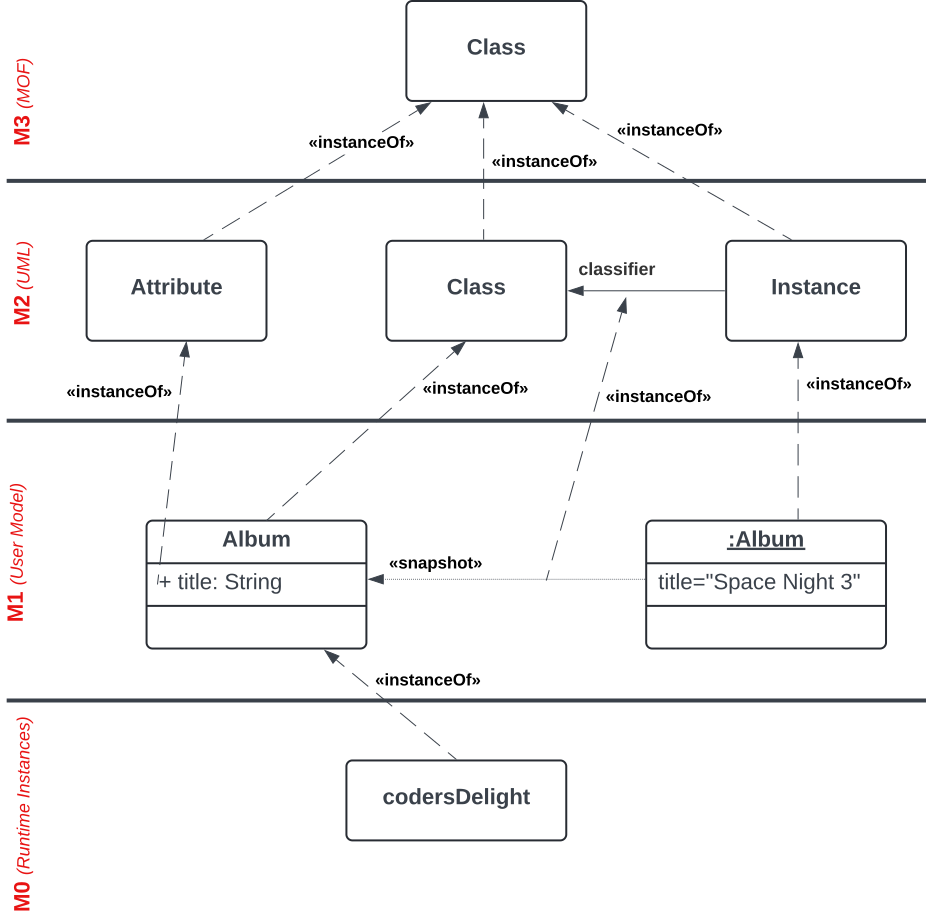
\includegraphics[scale=0.4]{part three/Einführung/img/metamodel}
    \caption{Beispiel für die verschiedenen Schichten der Metamodell Hierarchie.
        In der original Abbildung sind die Pfeilspitzen offen. (Quelle: in Anlehnung an S. 20, Figure 7.8, \url{https://www.omg.org/spec/UML/2.4.1/Infrastructure/PDF}, abgerufen 01.05.2024}
    \label{fig:metamodel-cc}
\end{figure}

\clearpage


\section{Strukturdiagramme}

\begin{tcolorbox}[title=Strukturdiagramme]
    In den \textbf{Strukturdiagrammen} werden \textbf{statische Strukturaspekte} eines Systems betrachtet.
    Für eine Systemmodellierung können alle dieser 6 Diagramme verwendet werden.

    \begin{itemize}
        \item \textbf{Klassendiagramm}: Das \textbf{Klassendiagramm} wird verwendet, um ein objektorientiertes System zu beschreiben.
        \item \textbf{Paketdiagramm}: Ein \textbf{Paketdiagramm} zeigt die Pakete eines Systems und deren Beziehungen.
        \item \textbf{Komponentendiagramm}: Stellt Komponenten oder auch \textit{Subsysteme} mit definierten Interfaces dar, um bspw. \textbf{Architekturdesign} darzustellen.
        \item \textbf{Verteilungsdiagramm}: Beschreibt eine Menge von Knoten, die die \textit{Ausführungsarchitektur} eines Systems definieren können, wobei Knoten i.d.R. \textit{Geräte} oder \textit{Softwareablaufumgebungen repräsentieren}.
        \item \textbf{Kompositionsstrukturdiagramm}: Stellt die \textbf{Komposition} von \textit{Systemstrukturen} (Klassen, Komponenten, Gesamtsystem) in einem bestimmten \textit{Kontext} mit einem bestimmten \textit{Ziel} dar (vgl. \cite[9]{Buh09}).
        \item \textbf{Objektdiagramm}: Momentaufnahme eines Systems zu genau einem \textit{Zeitpukt} während der Ausführung
    \end{itemize}

\end{tcolorbox}
\clearpage

\section{Verhaltensdiagramme}

\begin{tcolorbox}[title=Verhaltensdiagramme]
    \textbf{Verhaltensdiagramme} stellen \textit{Dynamik}, \textit{interne Abläufe} und das \textit{Zusammenspiel} der Systemteile dar, um eine Spezifikation zu vervollständigen.

    \begin{itemize}
        \item \textbf{Anwendungsfalldiagramm}: Dienen zur \textit{Spezifizierung} und \textit{Formalisierung} von \textit{Systemanforderungen}, unter Berücksichtigung von \textbf{Akteuren}, \textbf{Systemen} und \textbf{Anwendungsfällen}
        \item \textbf{Zustandsdiagramm}: Auch \textbf{Zustandsautomaten}; zeigen für ein einzelnes Objekt Zustandsänderungen während der Lebenszeit
        \item \textbf{Aktivitätsdiagramme}: Werden zur Modellierung von \textit{Kontroll}- oder \textit{Objektflüssen} oder zur Darstellung von \textit{Programmlogik} genutzt.
        \item \textbf{Interaktionsdiagramme}: Stellen das Zusammenspiel mehrerer Kommunikationspartner dar.
        Es gibt unterschiedliche Typen von Interaktionsdiagrammen, die Interaktionen auf verschiedenen \textit{Abstraktionsebenen} modellieren:
        \begin{itemize}
            \item \textbf{Sequenzdiagramm}: Zeigt den Verlauf einer Interaktion in zwei Dimensionen, \textit{Kommunikationspartner} und die Nachrichten in ihrer \textit{zeitlichen Abfolge}
            \item \textbf{Kommunikationsdiagramm}: hebt die Kommunikationsbeziehungen zwischen den Partnern hervor
            \item \textbf{Timing Diagramm}: hebt die zeitlichen Aspekte einer Interaktion hervor
            \item \textbf{Interaktionsüberblickdiagramm}: Spezialfall des \textbf{Aktivitätsdiagramms} - statt Aktionen und Aktivitäten können das \textbf{Sequenz}-, \textbf{Kommunikations}- und das \textbf{Timing}-Diagramm als Knoten verwendet werden.
        \end{itemize}
        Alle verwenden dieselben Grundelemente: \textit{Lebenslinien} der Akteure und Nachrichten, die zwischen diesen ausgetauscht werden.
    \end{itemize}
\end{tcolorbox}

\clearpage


\section{Klassendiagramm}

\begin{tcolorbox}[title=Klassendiagramm]
    Das \textbf{Klassendiagramm} beschreibt die Klassen eines Systems und die statischen Beziehungen zwischen ihnen.\\
    Sie werden in Form von Domainklassen bei der \textbf{Analyse} und als detaillierte Entwürfe von Systemklassen als \textit{Blueprint} im \textbf{gesamten Entwicklungsprozess} eingesetzt.

\end{tcolorbox}
\clearpage


\section{Assoziationsklasse (Attributierte Assoziation)}

\begin{tcolorbox}[title=Assoziationsklasse (Attributierte Assoziation)]
Eine \textbf{Assoziationsklasse} erlaubt das Hinzufügen von Operationen und Attributen zu einer Assoziation (\cite[43]{Buh09}).\\
Assoziationsklassen werden in der \textbf{Analyse} in Modellen verwendet und in dem \textbf{Entwurf} in eigenständige Klassen transformiert.\\

\noindent
Assoziationsklassen werden in der \textbf{Analyse} in Modellen verwendet und in dem \textbf{Entwurf} in eigenständige Klassen transformiert.

\blockquote[{\cite[277]{Oes05}}]{
    Eine attributierte Assoziation ist immer dann nahe liegend, wenn Attribute oder Operationen gefunden werden, die weder der einen noch der anderen Klasse zugeordnet werden können, weil sie nämlich Eigenschaften der Beziehung selbst sind.
}.\\

Bei einer attributierten Assoziation dürfen zwei beteiligte Objekte maximal nur eine Beziehung zueinander haben (vgl.~\cite[277]{Oes05})\footnote{
    \textit{Ostereich} führt dies ebenda auf Seite 278 weiter aus, in dem er beschreibt, wie eine attributierte Assoziation für ein \textit{Beschäftigtenverhältnis} zwischen \textit{Mitarbeiter} und \textit{Unternehmen} modelliert wird. Dabei wird davon ausgegangen, dass ein \textit{Mitarbeiter} nur über \textit{ein} Arbeitsverhältnis mit einem \textit{Unternehmen} in Beziehung stehen kann. Bestehen mehrere Arbeitsverhältnisse (\textit{Mitarbeiter} hat zu unterschiedlichen Zeitpunkten für das \textit{Unternehmen} gearbeitet), kann die attributierte Assoziation nicht verwendet werden.\\

\noindent
Wird eine attributierte Assoziation in eine gewöhnliche Assoziation transformiert, muss darauf geachtet werden, die Multiplizitäten richtig zu setzen (s. Abbildung~\ref{fig:assoziationsklasse}).
\end{tcolorbox}

\begin{figure}
    \centering
    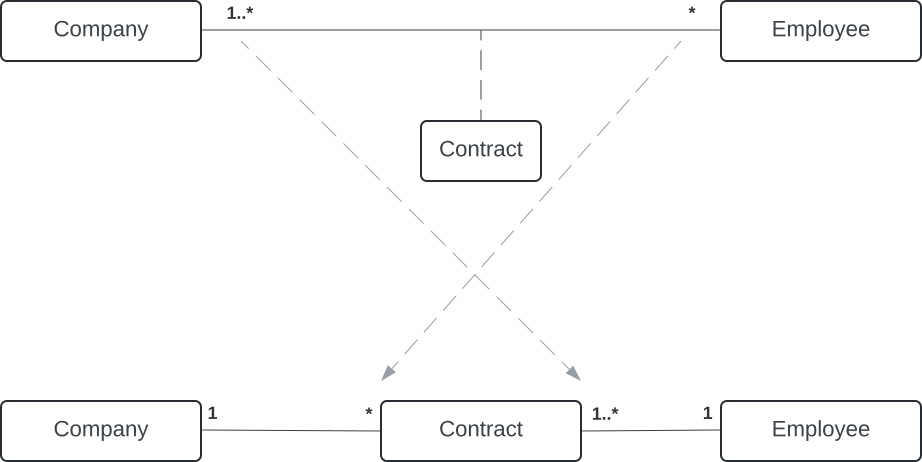
\includegraphics[scale=0.4]{part three/Klassendiagramme - Erweiterte Konzepte und Paketdiagramme/img/assoziationsklasse}
    \caption{Darstellung einer Assoziation mit Hilfe einer Assoziationsklasse (oben) sowie Transformation in gewöhnliche Assoziationen (unten). (Quelle: in Anlehnung an \cite[279, Abb. 4.4-11]{Oes05})}
    \label{fig:assoziationsklasse-cc}
\end{figure}

\clearpage


\section{Sequenzdiagramme}

\begin{tcolorbox}[title=Sequenzdiagramme]
    \textbf{Sequenzdiagramme} stellen Verhalten auf der Ebene einer Interaktion dar.\\
    In der Phase des Klassendesigns werden die Teilnehmer der Interaktionen bestimmt, weshalb Sequenzdiagramme oft in dieser Phase genutzt werden.\\
    In der \textbf{Analysephase} können Sequenzdiagramme eingesetzt werden, um die Kommunikation der bis dahin ausgemachten \textbf{Geschäftsobjekte} zu modellieren, oder um \textbf{Anwendungsfälle} weiter zu spezifizieren.
\end{tcolorbox}
\clearpage

\section{Aggregation}

\begin{tcolorbox}[title=Aggregation]
    Eine \textbf{Aggregation} ist in ihrer \semantischen Aussage unscharf (vgl.~\cite[40]{Buh09}).\\
    Sie beschreibt eine \textit{Ganzes}-\textit{Teile}-Beziehung, aber die \textit{Teile} können zu mehreren verschiedenen \textit{Ganzen} gehören.\\
    Außerdem kann ein Teil dem \textit{Ganzen} jederzeit wieder entnommen werden und das \textit{Ganze} ist nicht verantwortlich für das Erstellen der \textit{Teile}, weshalb Implementierungen beim Hinzufügen von Teilen oft schon fertige Objekte erwarten, die jeweils eines der \textit{Teile} repräsentieren.\\
    Aggregationsbeziehungen werden durch eine nicht-gefüllte Raute an der Seite der Klasse, die das Ganze repräsentiert, dargestellt.
\end{tcolorbox}
\clearpage

\section{Komposition}

\begin{tcolorbox}[title=Komposition]
    Bei einer \textbf{Komposition} handelt es sich um eine \textit{Ganzes}-\textit{Teile}-Beziehung, bei der das \textit{Ganze} verantwortlich für die Erstellung und Beseitigung der \textit{Teile} ist.
    Außerdem sind die \textit{Teile} an die \textbf{Existenz} des \textit{Ganzen} gebunden.\\
    \textit{Teile} gehören immer zu \textit{genau einem} \textit{Ganzen}.\\
    Eine Komposition wird dargestellt durch eine gefüllte Raute an der Klassenbox, die das \textit{Ganze} repräsentiert.
\end{tcolorbox}
\clearpage

\section{Paketdiagramm}

\begin{tcolorbox}[title=Komposition]
    \textbf{Paketdiagramme} zeigen Pakete und ihre Abhängigkeiten und werden in frühen Designphasen genutzt, um Strukturen (großer Systeme) aufzuzeigen.\\

    \noindent
    Elemente sollten so in Paketen gruppiert werden, dass ihr \textbf{funktionaler Zusammenhalt} (\textit{Kohäsion}, s. Abschnitt~\ref{subsec:hohe-kohasion}) klar wird.\\
    Hierdurch kann vermieden werden, dass Änderungen einer Klasse eines Paketes auch Änderungen außerhalb des Paketes erfordern.\\
    Außerdem erhöht sich die Wahrscheinlichkeit, dass einzelne Pakete als solche in anderen Projekten wiederverwendet werden können.\\

    \noindent
    In Paketdiagrammen können Beziehungen über folgende Schlüsselwörter deutlich gemacht werden:

    \begin{itemize}
        \item \guillemotleft import\guillemotright
        \item[] $\rightarrow$ \textbf{public-Import} zwischen Quell- und Zielpaket; Quellpaket kann die öffentlichen Elemente des Zielpaketes unter Verwendung des unqualifizierten und des qualifizierten Namens verwenden; die importierten Elemente sind auch für Pakete sichtbar, die das Quellpaket importieren
        \item \guillemotleft access\guillemotright
        \item[] $\rightarrow$ \textbf{privater Import} zwischen Quell- und Zielpaket; Zugriff auf Elemente des importierten Paketes ohne qualifizierenden Namen möglich; der Import eines Paketes in \textbf{Java} entspricht der \guillemotleft access\guillemotright-Beziehung
        \item \guillemotleft merge\guillemotright
        \item[] $\rightarrow$ Bei einem \textbf{merge} werden Elemente eines Zielpaketes in das Quellpaket
   \end{itemize}
\end{tcolorbox}
\clearpage

\section{Anwendungsfalldiagramm}

\begin{tcolorbox}[title=Anwendungsfalldiagramm]
    Die \textbf{Anwendungsfallanalyse} wird im Rahmen der \textbf{Anforderungsspezifikation} eingesetzt.\\

    \noindent
    Anwendungsfalldiagramme sind das am häufigsten eingesetzte Mittel zur Aufnahme und Darstellung von \textbf{Anforderungen}.\\
    Sie beschreiben selbst kein Verhalten und keine Abläufe, sondern zeigen nur die Zusammenhänge der an Anwendungsfällen beteiligten Modellelemente und sind somit ein Hilfsmittel zur Anforderungsermittlung und Verwaltung.\\

    \noindent
    Zu den wichtigsten Schritten einer Anwendungsfallanalyse gehören:
    \begin{enumerate}
        \item Akteure identifizieren
        \item Anwendungsfälle identifizieren
        \item Beschreiben der Akteure und Anwendungsfälle
        \item Identifizieren von \textit{Schlüsselobjekten}, die das System verwaltet
        \item Identifizieren der wichtigsten Anwendungsfälle (Priorisierung)
        \item detailliertere Beschreibung der Anwendungsfälle
        \item Strukturierung des Anwendungsfalldiagramms
    \end{enumerate}

    \noindent
    Anwendungsfälle beschreiben das \textbf{Szenario} der Nutzung, und nicht Features des Systems.
\end{tcolorbox}

\clearpage

\input{chapters/Anhang/CheatSheets/SE3/Aktivitätsdiagramm}
\clearpage

\section{Zustandsautomat}

\begin{tcolorbox}[title=Zustandsautomat]
    Mit \textbf{Zustandsautomaten} kann das \textit{Verhalten} von Systemen modelliert werden, wobei die \textit{Reaktionen} des Systems im Mittelpunkt stehen, und nicht die \textit{Aktionen}, wie bspw. bei den \textbf{Aktivitätsdiagrammen}.\\

    \noindent
        Ein \textbf{Zustandsautomat} kann den \textit{Lebensweg} eines Objektes modellieren, weshalb Zustandsautomaten oft im \textbf{Entwurf} als Ergänzung zu den \textbf{Klassendiagrammen} eingesetzt werden.
\end{tcolorbox}

\begin{figure}
    \centering
    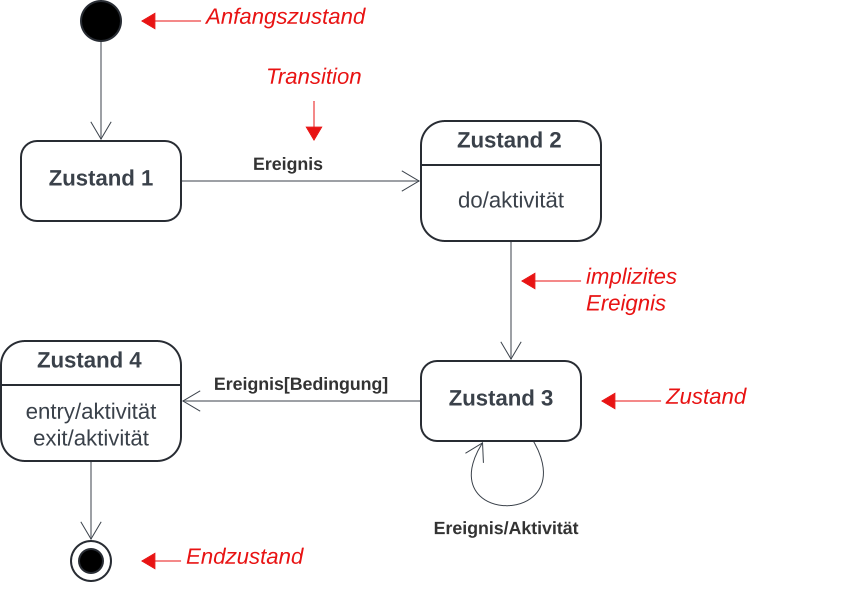
\includegraphics[scale=0.4]{part three/Zustandsautomaten/img/statechartdiagramnotation}
    \caption{Elemente eines einfachen Zustandsautomaten. Eine Transitionen wird durch ein \textbf{Ereignis} ausgelöst, das ein \textit{Signal}, ein \textit{Operationsaufruf} oder auch eine bestimmte \textit{Attributänderung} sein kann. (Quelle: in Anlehnung an \cite[90, Abb. 2.11-6]{Bal05})}
    \label{fig:statechartdiagramnotation-cc}
\end{figure}

\begin{minted}[fontsize=\small]{java}
// Beispiel für eine Implementierung eines
// Parkscheinautomaten als Zustandsautomat in Java
class Parkscheinautomat {

  // zustände
  private final int BEREIT = 0;
  private final int ZAHLUNG = 1;
  private final int ABBRUCH = 2;
  private final int BELEG   = 3;

  // Zustand; wird initial beim Starten
  // des Automaten gesetzt
  private int zustand;

  // Methoden lösen Aktionen beim Eintritt
  // in die jeweiligen Zustände aus
  private int zahlung() {
    // verarbeiten
    // danach neuen Zustand zurückliefern...
    ...
    return BEREIT;
  }

   ...

  private void bereit() {
    while (true) {
      // eingabe überprüfen und
      // ggf. Zustandswechsel auslösen:
      // Zustand als Attribut setzen
      ...
    }
  }

  public void start() {
    zustand = BEREIT;

    while(true) {
      switch (zustand) {
        case BEREIT:
          zustand = bereit();
        // ... weiteres Verhalten
        ...
      }
    }
  }
}
\end{minted}
\clearpage
	

\section{Inhalt SE3}

\section*{1. Übersicht UML}

\subsection*{Lernziele}
\begin{itemize}
    \item einen Einblick in den Sprachaufbau der UML 2.0 gewinnen
    \item einen Überblick über die Diagramme der UML 2.0 und deren Zweck haben
\end{itemize}

\subsection*{Zusammenfassung}
\begin{itemize}
    \item Die \textbf{UML} ist eine weit verbreitete Modellierungssprache zur Modellierung objektorientierter Softwaresysteme.
    \item Die UML 2.0 Spezifikation besteht aus vier Teilen:
    \begin{enumerate}
        \item \textbf{Superstructure}: Diagrammtypen
        \item \textbf{Infrastructure}: Modellierungskonzepte
        \item \textbf{OCL}: formale Sprache zur Formulierung von Einschränkungen
        \item \textbf{Diagram Interchange}: Austauschformate
    \end{enumerate}
    \item Die UML kann im \textbf{Sketching} oder \textbf{Blueprint Modus} eingesetzt werden, oder als Grundlage für \textbf{automatische Codegenerierung}
    \item Die UML ist an keinen speziellen Entwicklungsprozess gebunden
\end{itemize}

\section*{2. Klassendiagramme}

\subsection*{Lernziele}
\begin{itemize}
    \item wissen, wie Klassendiagramme im Entwicklungsprozess eingesetzt werden
    \item Klassendiagramme für Analyse- und Designentscheidungen einsetzen können
    \item die wichtigsten Modellierungskonzepte kennen
    \item sinnvolle Klassendiagramme erstellen und Java-Implementierungen ableiten können
    \item Klassendiagramme aus Java Quellcode erzeugen können
\end{itemize}

\subsection*{Zusammenfassung}

\begin{itemize}
    \item \textbf{Klassendiagramme} dienen zur \textbf{strukturellen Darstellung} von Softwaresystemen
    \item hierbei werden Klassen und \textbf{Beziehungen} zwischen Klassen dargestellt
    \item Properties können durch die \textbf{Attribut}- oder \textbf{Assoziationsnotation} modelliert werden
    \item Operationen werden als separate Zeile in ihrem Compartment dargestellt
    \item im Klassendiagramm können auch \textbf{Generalisierungsbeziehungen} modelliert werden
    \item \textbf{Abhängigkeitsbeziehungen} drücken ein Verhältnis zwischen \textbf{Client} und \textbf{Supplier} aus
\end{itemize}

\section*{3. Objektorientierter Entwurf}

\subsection*{Lernziele}
\begin{itemize}
    \item das Wesen einer Interaktion kennen
    \item wissen, wie Sequenzdiagramme im Entwicklungsprozess eingesetzt werden
    \item Sequenzdiagramme für Analyse- und Designentscheidungen sowie zur Darstellung von Kontrollflüssen einsetzen können
    \item die wichtigsten Modellierungskonzepte kennen
    \item sinnvolle Sequenzdiagramme erstellen und Java-Implementierungen ableiten können
    \item Sequenzdiagramme aus Java Quellcode erzeugen können
\end{itemize}

\subsection*{Zusammenfassung}

\begin{itemize}
    \item Sequenzdiagramme sind \textbf{Verhaltensdiagramme}
    und können im gesamten Entwicklungszyklus zur Modellierung von Interaktionen angewendet werden
    \item Interaktionen bestehen im Wesentlichen aus dem Nachrichtenaustausch zwischen verschiedenen Kommunikationspartnern
    \item in den meisten Fällen wird die Kommunikation von Objekten von Klassen modelliert, aber es können auch Teilnehmer auf anderen Ebenen modelliert werden
    \item gewöhnlich gibt ein Sequenzdiagramm einen \textbf{Anwendungsfall} (\textit{Szenario}) wieder
    \item sie dienen nicht dazu, um Zustandsänderungen darzustellen (hierfür werden Zustandsdiagramme verwendet)
    \item Sequenzdiagramme sind \textit{nicht} gut geeignet für die Darstellung von
    \begin{itemize}
        \item nebenläufigem Verhalten (\textit{asynchrone} Nachrichten, \textit{kombiniertes Fragment})
        \item Schleifen und alternativem Verhalten (\textit{kombinierte Fragmente})
        \item[] $\rightarrow$  für beide Fälle sind \textbf{Aktivitätsdiagramme} besser geeignet
    \end{itemize}
\end{itemize}

\section*{4. Klassendiagramme - Erweiterte Konzepte und Paketdiagramme}

\subsection*{Lernziele}
\begin{itemize}
    \item erweiterte Modellierungskonzepte in Klassendiagrammen für den Detailentwurf von Systemen kennen
    \item die Konsequenzen dieser Konzepte in der Implementierung kennen
    \item wissen, wie Paketdiagramme im Entwicklungsprozess eingesetzt werden
    \item die Modellierungskonzepte in Paketdiagrammen kennen
    \item anhand von Paketdiagrammen Software-Architekturen gestalten und bewerten können
\end{itemize}

\subsection*{Zusammenfassung}

\begin{itemize}
    \item Die vorgestellten erweiterten Konzepte werden vor allem im \textbf{Feinentwurf} von Klassenstrukturen eingesetzt.
    \item Generell gilt, dass die Spezifikationen von Objekten und Properties nur so detailliert ausgeführt werden sollen, wie nötig: Sind Details für das Verständnis unnötig, sollte darauf verzichtet werden.
    \item \textbf{Generalisierungsbeziehungen} sollten grundsätzlich modelliert werden.
    \item Ist eine \textbf{Komposition} statt einer Generalisierung für den Sachverhalt möglich, sollte diese verwendet werden: ``Favor object composition over inheritance.`` (\cite[19 f.]{GHJV94})
    \item \textbf{Kompositionsbeziehungen} geben eindeutige Impulse für eine Implementierung, \textbf{Aggregationsbeziehungen} sind in ihrer semantischen Aussage nicht sehr eindeutig
    \item \textbf{Assoziationsklassen} sind in ihrer frühen Designphase empfehlenswert, die Realisierung (mit {bspw.} Java) erfordert aber eine Transformation in eine volle Klasse, wobei die Multiplizitäten angepasst werden müssen
    \item Elemente können in \textbf{Paketen} zusamengefasst und unter einem gemeinsamen Namensraum gruppiert werden
\end{itemize}

\section*{4. Anwendungsfalldiagramm (Use-Case-Diagramm)}

\subsection*{Lernziele}
\begin{itemize}
    \item wissen, wie die Anwendungsfallanalyse im Rahmen der Anforderungsspezifikation eingesetzt wird
    \item Prozessschritte der Anwendungsfallanalyse beherrschen
    \item die wichtigsten Modellierungskonzepte in Anwendungsfalldiagrammen kennen
    \item den Aufbau einer Anwendungsfallbeschreibung kennen
\end{itemize}

\subsection*{Zusammenfassung}

\begin{itemize}
    \item \textbf{Anwendungsfalldiagramme} besitzen eine einfache Notation, um \textbf{Akteure} und \textbf{Anwendungsfälle} eines \textbf{Systems} grafisch darzustellen
    \item auf Basis eines Anwendungsfalldiagramms lässt sich ermitteln, ob die Anwendungsfälle gewünschtes Verhalten realisieren bzw. Beziehungen zu einem oder mehreren Akteuren haben
    \item Anwendungsfälle und Akteure \textit{müssen} zusätzlich textlich beschrieben werden
\end{itemize}

\section*{5. Aktivitätsdiagramme}

\subsection*{Lernziele}
\begin{itemize}
    \item wissen, wie Aktivitätsdiagramme im Rahmen der Verhaltensanalyse in verschiedenen Prozessphasen eingesetzt werden können
    \item die wichtigsten Modellierungskonzepte in Aktivitätsdiagrammen kennen
    \item Aktivitätsdiagramme interpretieren, erstellen und implementieren können
\end{itemize}

\subsection*{Zusammenfassung}

\begin{itemize}
    \item \textbf{Aktivitätsdiagramme} gehören zu den \textbf{Verhaltensdiagrammen} und können im \textit{gesamten} \textbf{Entwicklungsprozess} eingesetzt werden
    \item durch ein Aktivitätsdiagramm kann gezeigt werden, wie \textbf{Verhalten} realisiert wird
    \item es können mehrere \textbf{Aktivitäten} dargestellt werden
    \item \textbf{Aktivitätskanten} und \textbf{Aktivitätsknoten} werden zur Beschreibung von Verhalten verwendet
\end{itemize}

\section*{5. Zustandsautomaten}

\subsection*{Lernziele}
\begin{itemize}
    \item wissen, wie Zustandsdiagramme im Rahmen der Verhaltensanalyse einzelner Objekte eingesetzt werden können
    \item die wichtigsten Modellierungskonzepte in Zustandsdiagrammen kennen
    \item Zustandsdiagramme interpretieren, erstellen und implementieren können
\end{itemize}

\subsection*{Zusammenfassung}

\begin{itemize}
    \item Das \textbf{Zustandsdiagramm} gehört wie das \textbf{Aktivitätsdiagramm} zu den \textbf{Verhaltensdiagrammen}.
    \item Ein Zustandsdiagramm zeigt den \textbf{Lebensweg} eines \textbf{Objektes}.
    \item \textbf{Attributwerte} bestimmen den Zustand eines Objektes.
    \item \textbf{Transitionen} zwischen Zuständen werden durch \textbf{Guards} und \textbf{Events} gesteuert.
    \item Während der Transitionen können \textbf{Effekte} (\textit{Aktivitäten}) realisiert werden.
    \item Die Modellierung \textbf{zusammengesetzter Zustände} ist ebenfalls möglich.
    \item Für die Darstellung \textbf{paralleler} oder  \textbf{konkurrierender} Abläufe können \textbf{Regionen} modelliert werden.
\end{itemize}
\clearpage


\section{UML Modellierung}

\begin{tcolorbox}[title=UML Modellierung]
    \textbf{Modelle} haben die Aufgabe, den Bezug zum Original (Programm, Softwaresystem) herzustellen, sowie zu der \textit{Anwendungsumgebung}.\\
    Ein \textbf{Modell} enthält alle \textbf{Modellelemente}, die zur Beschreibung eines Softwaresystems nötig sind.\\

    \noindent
    Ein \textbf{Modellelement} wird als Element in einem UML Modell von einem Benutzer erstellt und auf verschiedenen \textbf{Diagrammen} (Struktur-/Verhaltensdiagrammen) platziert, und wird durch die \textbf{UML Modellierungskonzepte} als Metaklasse des \textbf{Metamodells} der UML beschrieben: \textbf{Modellelemente} werden aus Modellierungskonzepten instanziiert.\\

    \noindent
       Das \textbf{UML Metamodell} regelt, in welchem Zusammenhang \textbf{UML Modellierungskonzepte} in Modellen auftreten dürfen, und welche Eigenschaften und Beziehungen zu anderen Sprachelementen zulässig sind.\\

       \noindent
       Die im \textbf{Metamodell} verwendeten Erklärungen basieren auf einer abstrakten Syntax, für deren Beschreibung eine Untermenge (\textit{Klassendiagramme}) der UML verwendet wird.\\
        Die \textbf{Semantik} der Modellierungskonzepte wird textlich beschrieben, zur Formalisierung von Regeln für die syntaktische Korrektheit wird die \textbf{OCL} (\textit{Object Constraint Language}) verwendet.
\end{tcolorbox}

\begin{figure}
    \centering
    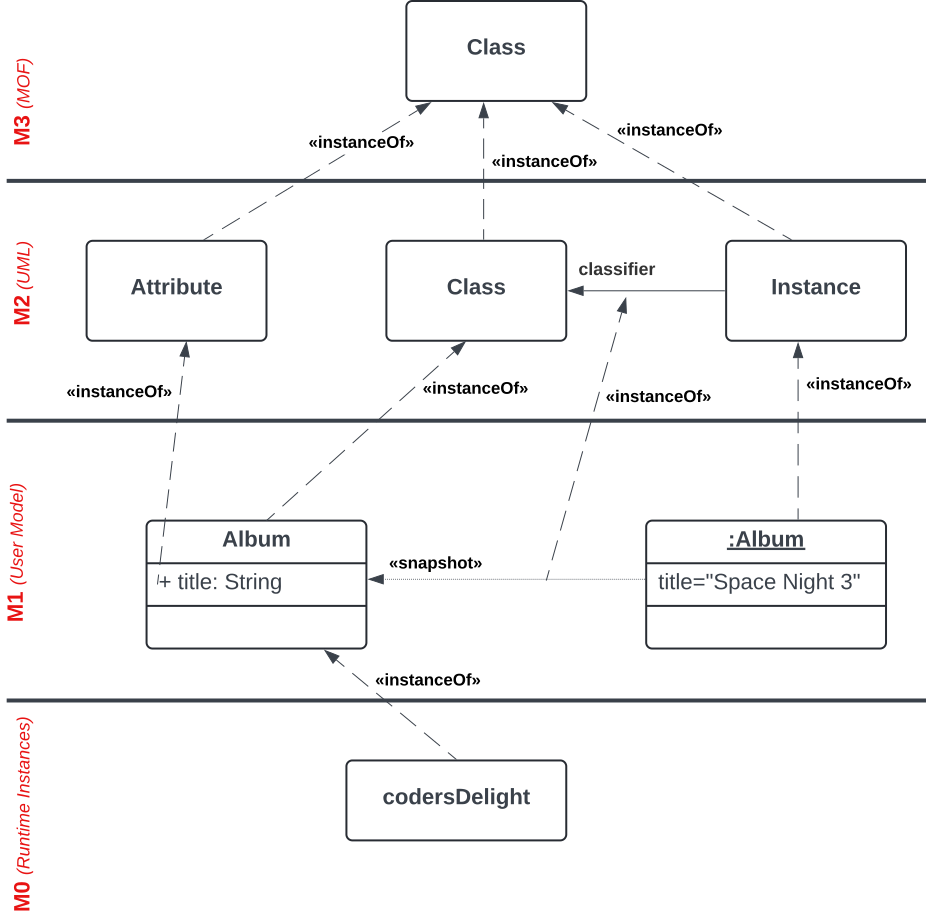
\includegraphics[scale=0.4]{part three/Einführung/img/metamodel}
    \caption{Beispiel für die verschiedenen Schichten der Metamodell Hierarchie.
        In der original Abbildung sind die Pfeilspitzen offen. (Quelle: in Anlehnung an S. 20, Figure 7.8, \url{https://www.omg.org/spec/UML/2.4.1/Infrastructure/PDF}, abgerufen 01.05.2024}
    \label{fig:metamodel-cc}
\end{figure}

\clearpage


\section{Strukturdiagramme}

\begin{tcolorbox}[title=Strukturdiagramme]
    In den \textbf{Strukturdiagrammen} werden \textbf{statische Strukturaspekte} eines Systems betrachtet.
    Für eine Systemmodellierung können alle dieser 6 Diagramme verwendet werden.

    \begin{itemize}
        \item \textbf{Klassendiagramm}: Das \textbf{Klassendiagramm} wird verwendet, um ein objektorientiertes System zu beschreiben.
        \item \textbf{Paketdiagramm}: Ein \textbf{Paketdiagramm} zeigt die Pakete eines Systems und deren Beziehungen.
        \item \textbf{Komponentendiagramm}: Stellt Komponenten oder auch \textit{Subsysteme} mit definierten Interfaces dar, um bspw. \textbf{Architekturdesign} darzustellen.
        \item \textbf{Verteilungsdiagramm}: Beschreibt eine Menge von Knoten, die die \textit{Ausführungsarchitektur} eines Systems definieren können, wobei Knoten i.d.R. \textit{Geräte} oder \textit{Softwareablaufumgebungen repräsentieren}.
        \item \textbf{Kompositionsstrukturdiagramm}: Stellt die \textbf{Komposition} von \textit{Systemstrukturen} (Klassen, Komponenten, Gesamtsystem) in einem bestimmten \textit{Kontext} mit einem bestimmten \textit{Ziel} dar (vgl. \cite[9]{Buh09}).
        \item \textbf{Objektdiagramm}: Momentaufnahme eines Systems zu genau einem \textit{Zeitpukt} während der Ausführung
    \end{itemize}

\end{tcolorbox}
\clearpage

\section{Verhaltensdiagramme}

\begin{tcolorbox}[title=Verhaltensdiagramme]
    \textbf{Verhaltensdiagramme} stellen \textit{Dynamik}, \textit{interne Abläufe} und das \textit{Zusammenspiel} der Systemteile dar, um eine Spezifikation zu vervollständigen.

    \begin{itemize}
        \item \textbf{Anwendungsfalldiagramm}: Dienen zur \textit{Spezifizierung} und \textit{Formalisierung} von \textit{Systemanforderungen}, unter Berücksichtigung von \textbf{Akteuren}, \textbf{Systemen} und \textbf{Anwendungsfällen}
        \item \textbf{Zustandsdiagramm}: Auch \textbf{Zustandsautomaten}; zeigen für ein einzelnes Objekt Zustandsänderungen während der Lebenszeit
        \item \textbf{Aktivitätsdiagramme}: Werden zur Modellierung von \textit{Kontroll}- oder \textit{Objektflüssen} oder zur Darstellung von \textit{Programmlogik} genutzt.
        \item \textbf{Interaktionsdiagramme}: Stellen das Zusammenspiel mehrerer Kommunikationspartner dar.
        Es gibt unterschiedliche Typen von Interaktionsdiagrammen, die Interaktionen auf verschiedenen \textit{Abstraktionsebenen} modellieren:
        \begin{itemize}
            \item \textbf{Sequenzdiagramm}: Zeigt den Verlauf einer Interaktion in zwei Dimensionen, \textit{Kommunikationspartner} und die Nachrichten in ihrer \textit{zeitlichen Abfolge}
            \item \textbf{Kommunikationsdiagramm}: hebt die Kommunikationsbeziehungen zwischen den Partnern hervor
            \item \textbf{Timing Diagramm}: hebt die zeitlichen Aspekte einer Interaktion hervor
            \item \textbf{Interaktionsüberblickdiagramm}: Spezialfall des \textbf{Aktivitätsdiagramms} - statt Aktionen und Aktivitäten können das \textbf{Sequenz}-, \textbf{Kommunikations}- und das \textbf{Timing}-Diagramm als Knoten verwendet werden.
        \end{itemize}
        Alle verwenden dieselben Grundelemente: \textit{Lebenslinien} der Akteure und Nachrichten, die zwischen diesen ausgetauscht werden.
    \end{itemize}
\end{tcolorbox}

\clearpage


\section{Klassendiagramm}

\begin{tcolorbox}[title=Klassendiagramm]
    Das \textbf{Klassendiagramm} beschreibt die Klassen eines Systems und die statischen Beziehungen zwischen ihnen.\\
    Sie werden in Form von Domainklassen bei der \textbf{Analyse} und als detaillierte Entwürfe von Systemklassen als \textit{Blueprint} im \textbf{gesamten Entwicklungsprozess} eingesetzt.

\end{tcolorbox}
\clearpage


\section{Assoziationsklasse (Attributierte Assoziation)}

\begin{tcolorbox}[title=Assoziationsklasse (Attributierte Assoziation)]
Eine \textbf{Assoziationsklasse} erlaubt das Hinzufügen von Operationen und Attributen zu einer Assoziation (\cite[43]{Buh09}).\\
Assoziationsklassen werden in der \textbf{Analyse} in Modellen verwendet und in dem \textbf{Entwurf} in eigenständige Klassen transformiert.\\

\noindent
Assoziationsklassen werden in der \textbf{Analyse} in Modellen verwendet und in dem \textbf{Entwurf} in eigenständige Klassen transformiert.

\blockquote[{\cite[277]{Oes05}}]{
    Eine attributierte Assoziation ist immer dann nahe liegend, wenn Attribute oder Operationen gefunden werden, die weder der einen noch der anderen Klasse zugeordnet werden können, weil sie nämlich Eigenschaften der Beziehung selbst sind.
}.\\

Bei einer attributierten Assoziation dürfen zwei beteiligte Objekte maximal nur eine Beziehung zueinander haben (vgl.~\cite[277]{Oes05})\footnote{
    \textit{Ostereich} führt dies ebenda auf Seite 278 weiter aus, in dem er beschreibt, wie eine attributierte Assoziation für ein \textit{Beschäftigtenverhältnis} zwischen \textit{Mitarbeiter} und \textit{Unternehmen} modelliert wird. Dabei wird davon ausgegangen, dass ein \textit{Mitarbeiter} nur über \textit{ein} Arbeitsverhältnis mit einem \textit{Unternehmen} in Beziehung stehen kann. Bestehen mehrere Arbeitsverhältnisse (\textit{Mitarbeiter} hat zu unterschiedlichen Zeitpunkten für das \textit{Unternehmen} gearbeitet), kann die attributierte Assoziation nicht verwendet werden.\\

\noindent
Wird eine attributierte Assoziation in eine gewöhnliche Assoziation transformiert, muss darauf geachtet werden, die Multiplizitäten richtig zu setzen (s. Abbildung~\ref{fig:assoziationsklasse}).
\end{tcolorbox}

\begin{figure}
    \centering
    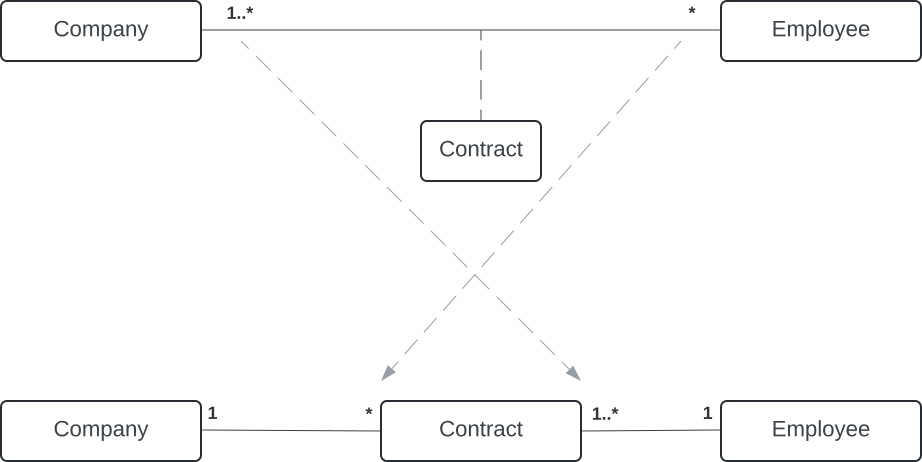
\includegraphics[scale=0.4]{part three/Klassendiagramme - Erweiterte Konzepte und Paketdiagramme/img/assoziationsklasse}
    \caption{Darstellung einer Assoziation mit Hilfe einer Assoziationsklasse (oben) sowie Transformation in gewöhnliche Assoziationen (unten). (Quelle: in Anlehnung an \cite[279, Abb. 4.4-11]{Oes05})}
    \label{fig:assoziationsklasse-cc}
\end{figure}

\clearpage


\section{Sequenzdiagramme}

\begin{tcolorbox}[title=Sequenzdiagramme]
    \textbf{Sequenzdiagramme} stellen Verhalten auf der Ebene einer Interaktion dar.\\
    In der Phase des Klassendesigns werden die Teilnehmer der Interaktionen bestimmt, weshalb Sequenzdiagramme oft in dieser Phase genutzt werden.\\
    In der \textbf{Analysephase} können Sequenzdiagramme eingesetzt werden, um die Kommunikation der bis dahin ausgemachten \textbf{Geschäftsobjekte} zu modellieren, oder um \textbf{Anwendungsfälle} weiter zu spezifizieren.
\end{tcolorbox}
\clearpage

\section{Aggregation}

\begin{tcolorbox}[title=Aggregation]
    Eine \textbf{Aggregation} ist in ihrer \semantischen Aussage unscharf (vgl.~\cite[40]{Buh09}).\\
    Sie beschreibt eine \textit{Ganzes}-\textit{Teile}-Beziehung, aber die \textit{Teile} können zu mehreren verschiedenen \textit{Ganzen} gehören.\\
    Außerdem kann ein Teil dem \textit{Ganzen} jederzeit wieder entnommen werden und das \textit{Ganze} ist nicht verantwortlich für das Erstellen der \textit{Teile}, weshalb Implementierungen beim Hinzufügen von Teilen oft schon fertige Objekte erwarten, die jeweils eines der \textit{Teile} repräsentieren.\\
    Aggregationsbeziehungen werden durch eine nicht-gefüllte Raute an der Seite der Klasse, die das Ganze repräsentiert, dargestellt.
\end{tcolorbox}
\clearpage

\section{Komposition}

\begin{tcolorbox}[title=Komposition]
    Bei einer \textbf{Komposition} handelt es sich um eine \textit{Ganzes}-\textit{Teile}-Beziehung, bei der das \textit{Ganze} verantwortlich für die Erstellung und Beseitigung der \textit{Teile} ist.
    Außerdem sind die \textit{Teile} an die \textbf{Existenz} des \textit{Ganzen} gebunden.\\
    \textit{Teile} gehören immer zu \textit{genau einem} \textit{Ganzen}.\\
    Eine Komposition wird dargestellt durch eine gefüllte Raute an der Klassenbox, die das \textit{Ganze} repräsentiert.
\end{tcolorbox}
\clearpage

\section{Paketdiagramm}

\begin{tcolorbox}[title=Komposition]
    \textbf{Paketdiagramme} zeigen Pakete und ihre Abhängigkeiten und werden in frühen Designphasen genutzt, um Strukturen (großer Systeme) aufzuzeigen.\\

    \noindent
    Elemente sollten so in Paketen gruppiert werden, dass ihr \textbf{funktionaler Zusammenhalt} (\textit{Kohäsion}, s. Abschnitt~\ref{subsec:hohe-kohasion}) klar wird.\\
    Hierdurch kann vermieden werden, dass Änderungen einer Klasse eines Paketes auch Änderungen außerhalb des Paketes erfordern.\\
    Außerdem erhöht sich die Wahrscheinlichkeit, dass einzelne Pakete als solche in anderen Projekten wiederverwendet werden können.\\

    \noindent
    In Paketdiagrammen können Beziehungen über folgende Schlüsselwörter deutlich gemacht werden:

    \begin{itemize}
        \item \guillemotleft import\guillemotright
        \item[] $\rightarrow$ \textbf{public-Import} zwischen Quell- und Zielpaket; Quellpaket kann die öffentlichen Elemente des Zielpaketes unter Verwendung des unqualifizierten und des qualifizierten Namens verwenden; die importierten Elemente sind auch für Pakete sichtbar, die das Quellpaket importieren
        \item \guillemotleft access\guillemotright
        \item[] $\rightarrow$ \textbf{privater Import} zwischen Quell- und Zielpaket; Zugriff auf Elemente des importierten Paketes ohne qualifizierenden Namen möglich; der Import eines Paketes in \textbf{Java} entspricht der \guillemotleft access\guillemotright-Beziehung
        \item \guillemotleft merge\guillemotright
        \item[] $\rightarrow$ Bei einem \textbf{merge} werden Elemente eines Zielpaketes in das Quellpaket
   \end{itemize}
\end{tcolorbox}
\clearpage

\section{Anwendungsfalldiagramm}

\begin{tcolorbox}[title=Anwendungsfalldiagramm]
    Die \textbf{Anwendungsfallanalyse} wird im Rahmen der \textbf{Anforderungsspezifikation} eingesetzt.\\

    \noindent
    Anwendungsfalldiagramme sind das am häufigsten eingesetzte Mittel zur Aufnahme und Darstellung von \textbf{Anforderungen}.\\
    Sie beschreiben selbst kein Verhalten und keine Abläufe, sondern zeigen nur die Zusammenhänge der an Anwendungsfällen beteiligten Modellelemente und sind somit ein Hilfsmittel zur Anforderungsermittlung und Verwaltung.\\

    \noindent
    Zu den wichtigsten Schritten einer Anwendungsfallanalyse gehören:
    \begin{enumerate}
        \item Akteure identifizieren
        \item Anwendungsfälle identifizieren
        \item Beschreiben der Akteure und Anwendungsfälle
        \item Identifizieren von \textit{Schlüsselobjekten}, die das System verwaltet
        \item Identifizieren der wichtigsten Anwendungsfälle (Priorisierung)
        \item detailliertere Beschreibung der Anwendungsfälle
        \item Strukturierung des Anwendungsfalldiagramms
    \end{enumerate}

    \noindent
    Anwendungsfälle beschreiben das \textbf{Szenario} der Nutzung, und nicht Features des Systems.
\end{tcolorbox}

\clearpage

\input{chapters/Anhang/CheatSheets/SE3/Aktivitätsdiagramm}
\clearpage

\section{Zustandsautomat}

\begin{tcolorbox}[title=Zustandsautomat]
    Mit \textbf{Zustandsautomaten} kann das \textit{Verhalten} von Systemen modelliert werden, wobei die \textit{Reaktionen} des Systems im Mittelpunkt stehen, und nicht die \textit{Aktionen}, wie bspw. bei den \textbf{Aktivitätsdiagrammen}.\\

    \noindent
        Ein \textbf{Zustandsautomat} kann den \textit{Lebensweg} eines Objektes modellieren, weshalb Zustandsautomaten oft im \textbf{Entwurf} als Ergänzung zu den \textbf{Klassendiagrammen} eingesetzt werden.
\end{tcolorbox}

\begin{figure}
    \centering
    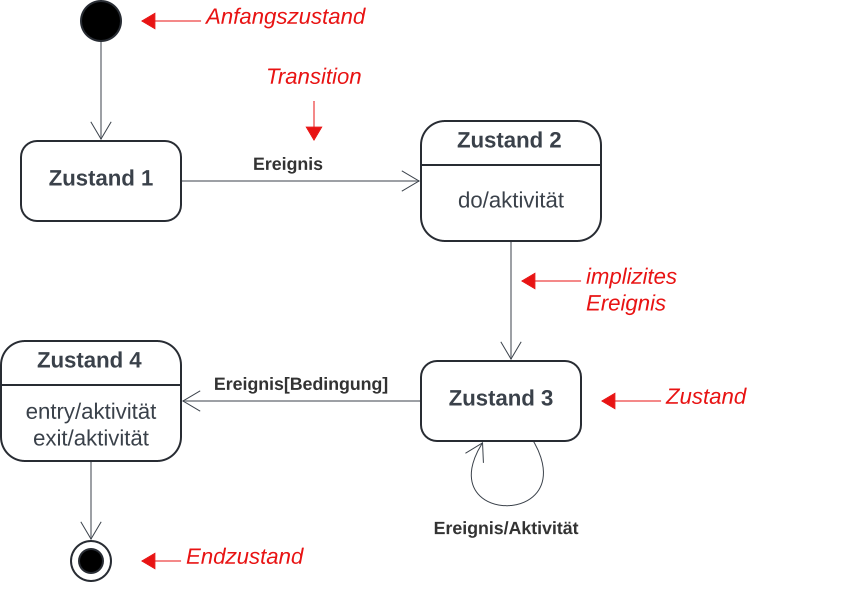
\includegraphics[scale=0.4]{part three/Zustandsautomaten/img/statechartdiagramnotation}
    \caption{Elemente eines einfachen Zustandsautomaten. Eine Transitionen wird durch ein \textbf{Ereignis} ausgelöst, das ein \textit{Signal}, ein \textit{Operationsaufruf} oder auch eine bestimmte \textit{Attributänderung} sein kann. (Quelle: in Anlehnung an \cite[90, Abb. 2.11-6]{Bal05})}
    \label{fig:statechartdiagramnotation-cc}
\end{figure}

\begin{minted}[fontsize=\small]{java}
// Beispiel für eine Implementierung eines
// Parkscheinautomaten als Zustandsautomat in Java
class Parkscheinautomat {

  // zustände
  private final int BEREIT = 0;
  private final int ZAHLUNG = 1;
  private final int ABBRUCH = 2;
  private final int BELEG   = 3;

  // Zustand; wird initial beim Starten
  // des Automaten gesetzt
  private int zustand;

  // Methoden lösen Aktionen beim Eintritt
  // in die jeweiligen Zustände aus
  private int zahlung() {
    // verarbeiten
    // danach neuen Zustand zurückliefern...
    ...
    return BEREIT;
  }

   ...

  private void bereit() {
    while (true) {
      // eingabe überprüfen und
      // ggf. Zustandswechsel auslösen:
      // Zustand als Attribut setzen
      ...
    }
  }

  public void start() {
    zustand = BEREIT;

    while(true) {
      switch (zustand) {
        case BEREIT:
          zustand = bereit();
        // ... weiteres Verhalten
        ...
      }
    }
  }
}
\end{minted}
\clearpage
	

\section{Inhalt SE3}

\section*{1. Übersicht UML}

\subsection*{Lernziele}
\begin{itemize}
    \item einen Einblick in den Sprachaufbau der UML 2.0 gewinnen
    \item einen Überblick über die Diagramme der UML 2.0 und deren Zweck haben
\end{itemize}

\subsection*{Zusammenfassung}
\begin{itemize}
    \item Die \textbf{UML} ist eine weit verbreitete Modellierungssprache zur Modellierung objektorientierter Softwaresysteme.
    \item Die UML 2.0 Spezifikation besteht aus vier Teilen:
    \begin{enumerate}
        \item \textbf{Superstructure}: Diagrammtypen
        \item \textbf{Infrastructure}: Modellierungskonzepte
        \item \textbf{OCL}: formale Sprache zur Formulierung von Einschränkungen
        \item \textbf{Diagram Interchange}: Austauschformate
    \end{enumerate}
    \item Die UML kann im \textbf{Sketching} oder \textbf{Blueprint Modus} eingesetzt werden, oder als Grundlage für \textbf{automatische Codegenerierung}
    \item Die UML ist an keinen speziellen Entwicklungsprozess gebunden
\end{itemize}

\section*{2. Klassendiagramme}

\subsection*{Lernziele}
\begin{itemize}
    \item wissen, wie Klassendiagramme im Entwicklungsprozess eingesetzt werden
    \item Klassendiagramme für Analyse- und Designentscheidungen einsetzen können
    \item die wichtigsten Modellierungskonzepte kennen
    \item sinnvolle Klassendiagramme erstellen und Java-Implementierungen ableiten können
    \item Klassendiagramme aus Java Quellcode erzeugen können
\end{itemize}

\subsection*{Zusammenfassung}

\begin{itemize}
    \item \textbf{Klassendiagramme} dienen zur \textbf{strukturellen Darstellung} von Softwaresystemen
    \item hierbei werden Klassen und \textbf{Beziehungen} zwischen Klassen dargestellt
    \item Properties können durch die \textbf{Attribut}- oder \textbf{Assoziationsnotation} modelliert werden
    \item Operationen werden als separate Zeile in ihrem Compartment dargestellt
    \item im Klassendiagramm können auch \textbf{Generalisierungsbeziehungen} modelliert werden
    \item \textbf{Abhängigkeitsbeziehungen} drücken ein Verhältnis zwischen \textbf{Client} und \textbf{Supplier} aus
\end{itemize}

\section*{3. Objektorientierter Entwurf}

\subsection*{Lernziele}
\begin{itemize}
    \item das Wesen einer Interaktion kennen
    \item wissen, wie Sequenzdiagramme im Entwicklungsprozess eingesetzt werden
    \item Sequenzdiagramme für Analyse- und Designentscheidungen sowie zur Darstellung von Kontrollflüssen einsetzen können
    \item die wichtigsten Modellierungskonzepte kennen
    \item sinnvolle Sequenzdiagramme erstellen und Java-Implementierungen ableiten können
    \item Sequenzdiagramme aus Java Quellcode erzeugen können
\end{itemize}

\subsection*{Zusammenfassung}

\begin{itemize}
    \item Sequenzdiagramme sind \textbf{Verhaltensdiagramme}
    und können im gesamten Entwicklungszyklus zur Modellierung von Interaktionen angewendet werden
    \item Interaktionen bestehen im Wesentlichen aus dem Nachrichtenaustausch zwischen verschiedenen Kommunikationspartnern
    \item in den meisten Fällen wird die Kommunikation von Objekten von Klassen modelliert, aber es können auch Teilnehmer auf anderen Ebenen modelliert werden
    \item gewöhnlich gibt ein Sequenzdiagramm einen \textbf{Anwendungsfall} (\textit{Szenario}) wieder
    \item sie dienen nicht dazu, um Zustandsänderungen darzustellen (hierfür werden Zustandsdiagramme verwendet)
    \item Sequenzdiagramme sind \textit{nicht} gut geeignet für die Darstellung von
    \begin{itemize}
        \item nebenläufigem Verhalten (\textit{asynchrone} Nachrichten, \textit{kombiniertes Fragment})
        \item Schleifen und alternativem Verhalten (\textit{kombinierte Fragmente})
        \item[] $\rightarrow$  für beide Fälle sind \textbf{Aktivitätsdiagramme} besser geeignet
    \end{itemize}
\end{itemize}

\section*{4. Klassendiagramme - Erweiterte Konzepte und Paketdiagramme}

\subsection*{Lernziele}
\begin{itemize}
    \item erweiterte Modellierungskonzepte in Klassendiagrammen für den Detailentwurf von Systemen kennen
    \item die Konsequenzen dieser Konzepte in der Implementierung kennen
    \item wissen, wie Paketdiagramme im Entwicklungsprozess eingesetzt werden
    \item die Modellierungskonzepte in Paketdiagrammen kennen
    \item anhand von Paketdiagrammen Software-Architekturen gestalten und bewerten können
\end{itemize}

\subsection*{Zusammenfassung}

\begin{itemize}
    \item Die vorgestellten erweiterten Konzepte werden vor allem im \textbf{Feinentwurf} von Klassenstrukturen eingesetzt.
    \item Generell gilt, dass die Spezifikationen von Objekten und Properties nur so detailliert ausgeführt werden sollen, wie nötig: Sind Details für das Verständnis unnötig, sollte darauf verzichtet werden.
    \item \textbf{Generalisierungsbeziehungen} sollten grundsätzlich modelliert werden.
    \item Ist eine \textbf{Komposition} statt einer Generalisierung für den Sachverhalt möglich, sollte diese verwendet werden: ``Favor object composition over inheritance.`` (\cite[19 f.]{GHJV94})
    \item \textbf{Kompositionsbeziehungen} geben eindeutige Impulse für eine Implementierung, \textbf{Aggregationsbeziehungen} sind in ihrer semantischen Aussage nicht sehr eindeutig
    \item \textbf{Assoziationsklassen} sind in ihrer frühen Designphase empfehlenswert, die Realisierung (mit {bspw.} Java) erfordert aber eine Transformation in eine volle Klasse, wobei die Multiplizitäten angepasst werden müssen
    \item Elemente können in \textbf{Paketen} zusamengefasst und unter einem gemeinsamen Namensraum gruppiert werden
\end{itemize}

\section*{4. Anwendungsfalldiagramm (Use-Case-Diagramm)}

\subsection*{Lernziele}
\begin{itemize}
    \item wissen, wie die Anwendungsfallanalyse im Rahmen der Anforderungsspezifikation eingesetzt wird
    \item Prozessschritte der Anwendungsfallanalyse beherrschen
    \item die wichtigsten Modellierungskonzepte in Anwendungsfalldiagrammen kennen
    \item den Aufbau einer Anwendungsfallbeschreibung kennen
\end{itemize}

\subsection*{Zusammenfassung}

\begin{itemize}
    \item \textbf{Anwendungsfalldiagramme} besitzen eine einfache Notation, um \textbf{Akteure} und \textbf{Anwendungsfälle} eines \textbf{Systems} grafisch darzustellen
    \item auf Basis eines Anwendungsfalldiagramms lässt sich ermitteln, ob die Anwendungsfälle gewünschtes Verhalten realisieren bzw. Beziehungen zu einem oder mehreren Akteuren haben
    \item Anwendungsfälle und Akteure \textit{müssen} zusätzlich textlich beschrieben werden
\end{itemize}

\section*{5. Aktivitätsdiagramme}

\subsection*{Lernziele}
\begin{itemize}
    \item wissen, wie Aktivitätsdiagramme im Rahmen der Verhaltensanalyse in verschiedenen Prozessphasen eingesetzt werden können
    \item die wichtigsten Modellierungskonzepte in Aktivitätsdiagrammen kennen
    \item Aktivitätsdiagramme interpretieren, erstellen und implementieren können
\end{itemize}

\subsection*{Zusammenfassung}

\begin{itemize}
    \item \textbf{Aktivitätsdiagramme} gehören zu den \textbf{Verhaltensdiagrammen} und können im \textit{gesamten} \textbf{Entwicklungsprozess} eingesetzt werden
    \item durch ein Aktivitätsdiagramm kann gezeigt werden, wie \textbf{Verhalten} realisiert wird
    \item es können mehrere \textbf{Aktivitäten} dargestellt werden
    \item \textbf{Aktivitätskanten} und \textbf{Aktivitätsknoten} werden zur Beschreibung von Verhalten verwendet
\end{itemize}

\section*{5. Zustandsautomaten}

\subsection*{Lernziele}
\begin{itemize}
    \item wissen, wie Zustandsdiagramme im Rahmen der Verhaltensanalyse einzelner Objekte eingesetzt werden können
    \item die wichtigsten Modellierungskonzepte in Zustandsdiagrammen kennen
    \item Zustandsdiagramme interpretieren, erstellen und implementieren können
\end{itemize}

\subsection*{Zusammenfassung}

\begin{itemize}
    \item Das \textbf{Zustandsdiagramm} gehört wie das \textbf{Aktivitätsdiagramm} zu den \textbf{Verhaltensdiagrammen}.
    \item Ein Zustandsdiagramm zeigt den \textbf{Lebensweg} eines \textbf{Objektes}.
    \item \textbf{Attributwerte} bestimmen den Zustand eines Objektes.
    \item \textbf{Transitionen} zwischen Zuständen werden durch \textbf{Guards} und \textbf{Events} gesteuert.
    \item Während der Transitionen können \textbf{Effekte} (\textit{Aktivitäten}) realisiert werden.
    \item Die Modellierung \textbf{zusammengesetzter Zustände} ist ebenfalls möglich.
    \item Für die Darstellung \textbf{paralleler} oder  \textbf{konkurrierender} Abläufe können \textbf{Regionen} modelliert werden.
\end{itemize}
\clearpage


\section{UML Modellierung}

\begin{tcolorbox}[title=UML Modellierung]
    \textbf{Modelle} haben die Aufgabe, den Bezug zum Original (Programm, Softwaresystem) herzustellen, sowie zu der \textit{Anwendungsumgebung}.\\
    Ein \textbf{Modell} enthält alle \textbf{Modellelemente}, die zur Beschreibung eines Softwaresystems nötig sind.\\

    \noindent
    Ein \textbf{Modellelement} wird als Element in einem UML Modell von einem Benutzer erstellt und auf verschiedenen \textbf{Diagrammen} (Struktur-/Verhaltensdiagrammen) platziert, und wird durch die \textbf{UML Modellierungskonzepte} als Metaklasse des \textbf{Metamodells} der UML beschrieben: \textbf{Modellelemente} werden aus Modellierungskonzepten instanziiert.\\

    \noindent
       Das \textbf{UML Metamodell} regelt, in welchem Zusammenhang \textbf{UML Modellierungskonzepte} in Modellen auftreten dürfen, und welche Eigenschaften und Beziehungen zu anderen Sprachelementen zulässig sind.\\

       \noindent
       Die im \textbf{Metamodell} verwendeten Erklärungen basieren auf einer abstrakten Syntax, für deren Beschreibung eine Untermenge (\textit{Klassendiagramme}) der UML verwendet wird.\\
        Die \textbf{Semantik} der Modellierungskonzepte wird textlich beschrieben, zur Formalisierung von Regeln für die syntaktische Korrektheit wird die \textbf{OCL} (\textit{Object Constraint Language}) verwendet.
\end{tcolorbox}

\begin{figure}
    \centering
    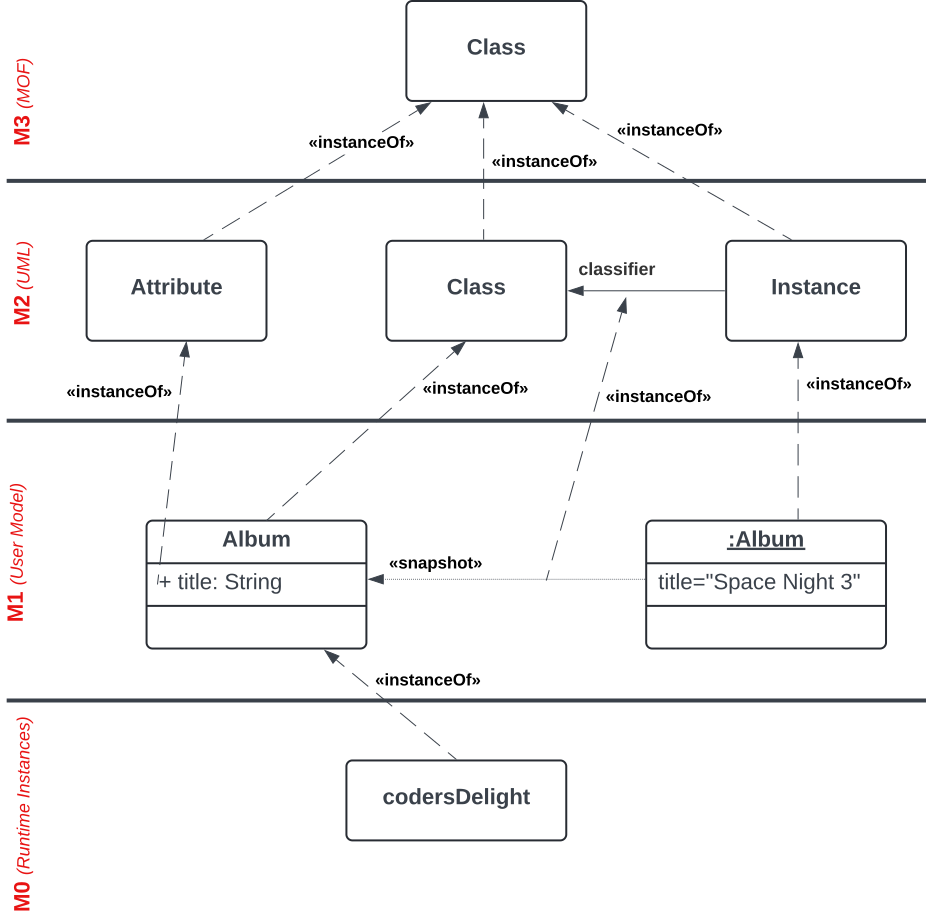
\includegraphics[scale=0.4]{part three/Einführung/img/metamodel}
    \caption{Beispiel für die verschiedenen Schichten der Metamodell Hierarchie.
        In der original Abbildung sind die Pfeilspitzen offen. (Quelle: in Anlehnung an S. 20, Figure 7.8, \url{https://www.omg.org/spec/UML/2.4.1/Infrastructure/PDF}, abgerufen 01.05.2024}
    \label{fig:metamodel-cc}
\end{figure}

\clearpage


\section{Strukturdiagramme}

\begin{tcolorbox}[title=Strukturdiagramme]
    In den \textbf{Strukturdiagrammen} werden \textbf{statische Strukturaspekte} eines Systems betrachtet.
    Für eine Systemmodellierung können alle dieser 6 Diagramme verwendet werden.

    \begin{itemize}
        \item \textbf{Klassendiagramm}: Das \textbf{Klassendiagramm} wird verwendet, um ein objektorientiertes System zu beschreiben.
        \item \textbf{Paketdiagramm}: Ein \textbf{Paketdiagramm} zeigt die Pakete eines Systems und deren Beziehungen.
        \item \textbf{Komponentendiagramm}: Stellt Komponenten oder auch \textit{Subsysteme} mit definierten Interfaces dar, um bspw. \textbf{Architekturdesign} darzustellen.
        \item \textbf{Verteilungsdiagramm}: Beschreibt eine Menge von Knoten, die die \textit{Ausführungsarchitektur} eines Systems definieren können, wobei Knoten i.d.R. \textit{Geräte} oder \textit{Softwareablaufumgebungen repräsentieren}.
        \item \textbf{Kompositionsstrukturdiagramm}: Stellt die \textbf{Komposition} von \textit{Systemstrukturen} (Klassen, Komponenten, Gesamtsystem) in einem bestimmten \textit{Kontext} mit einem bestimmten \textit{Ziel} dar (vgl. \cite[9]{Buh09}).
        \item \textbf{Objektdiagramm}: Momentaufnahme eines Systems zu genau einem \textit{Zeitpukt} während der Ausführung
    \end{itemize}

\end{tcolorbox}
\clearpage

\section{Verhaltensdiagramme}

\begin{tcolorbox}[title=Verhaltensdiagramme]
    \textbf{Verhaltensdiagramme} stellen \textit{Dynamik}, \textit{interne Abläufe} und das \textit{Zusammenspiel} der Systemteile dar, um eine Spezifikation zu vervollständigen.

    \begin{itemize}
        \item \textbf{Anwendungsfalldiagramm}: Dienen zur \textit{Spezifizierung} und \textit{Formalisierung} von \textit{Systemanforderungen}, unter Berücksichtigung von \textbf{Akteuren}, \textbf{Systemen} und \textbf{Anwendungsfällen}
        \item \textbf{Zustandsdiagramm}: Auch \textbf{Zustandsautomaten}; zeigen für ein einzelnes Objekt Zustandsänderungen während der Lebenszeit
        \item \textbf{Aktivitätsdiagramme}: Werden zur Modellierung von \textit{Kontroll}- oder \textit{Objektflüssen} oder zur Darstellung von \textit{Programmlogik} genutzt.
        \item \textbf{Interaktionsdiagramme}: Stellen das Zusammenspiel mehrerer Kommunikationspartner dar.
        Es gibt unterschiedliche Typen von Interaktionsdiagrammen, die Interaktionen auf verschiedenen \textit{Abstraktionsebenen} modellieren:
        \begin{itemize}
            \item \textbf{Sequenzdiagramm}: Zeigt den Verlauf einer Interaktion in zwei Dimensionen, \textit{Kommunikationspartner} und die Nachrichten in ihrer \textit{zeitlichen Abfolge}
            \item \textbf{Kommunikationsdiagramm}: hebt die Kommunikationsbeziehungen zwischen den Partnern hervor
            \item \textbf{Timing Diagramm}: hebt die zeitlichen Aspekte einer Interaktion hervor
            \item \textbf{Interaktionsüberblickdiagramm}: Spezialfall des \textbf{Aktivitätsdiagramms} - statt Aktionen und Aktivitäten können das \textbf{Sequenz}-, \textbf{Kommunikations}- und das \textbf{Timing}-Diagramm als Knoten verwendet werden.
        \end{itemize}
        Alle verwenden dieselben Grundelemente: \textit{Lebenslinien} der Akteure und Nachrichten, die zwischen diesen ausgetauscht werden.
    \end{itemize}
\end{tcolorbox}

\clearpage


\section{Klassendiagramm}

\begin{tcolorbox}[title=Klassendiagramm]
    Das \textbf{Klassendiagramm} beschreibt die Klassen eines Systems und die statischen Beziehungen zwischen ihnen.\\
    Sie werden in Form von Domainklassen bei der \textbf{Analyse} und als detaillierte Entwürfe von Systemklassen als \textit{Blueprint} im \textbf{gesamten Entwicklungsprozess} eingesetzt.

\end{tcolorbox}
\clearpage


\section{Assoziationsklasse (Attributierte Assoziation)}

\begin{tcolorbox}[title=Assoziationsklasse (Attributierte Assoziation)]
Eine \textbf{Assoziationsklasse} erlaubt das Hinzufügen von Operationen und Attributen zu einer Assoziation (\cite[43]{Buh09}).\\
Assoziationsklassen werden in der \textbf{Analyse} in Modellen verwendet und in dem \textbf{Entwurf} in eigenständige Klassen transformiert.\\

\noindent
Assoziationsklassen werden in der \textbf{Analyse} in Modellen verwendet und in dem \textbf{Entwurf} in eigenständige Klassen transformiert.

\blockquote[{\cite[277]{Oes05}}]{
    Eine attributierte Assoziation ist immer dann nahe liegend, wenn Attribute oder Operationen gefunden werden, die weder der einen noch der anderen Klasse zugeordnet werden können, weil sie nämlich Eigenschaften der Beziehung selbst sind.
}.\\

Bei einer attributierten Assoziation dürfen zwei beteiligte Objekte maximal nur eine Beziehung zueinander haben (vgl.~\cite[277]{Oes05})\footnote{
    \textit{Ostereich} führt dies ebenda auf Seite 278 weiter aus, in dem er beschreibt, wie eine attributierte Assoziation für ein \textit{Beschäftigtenverhältnis} zwischen \textit{Mitarbeiter} und \textit{Unternehmen} modelliert wird. Dabei wird davon ausgegangen, dass ein \textit{Mitarbeiter} nur über \textit{ein} Arbeitsverhältnis mit einem \textit{Unternehmen} in Beziehung stehen kann. Bestehen mehrere Arbeitsverhältnisse (\textit{Mitarbeiter} hat zu unterschiedlichen Zeitpunkten für das \textit{Unternehmen} gearbeitet), kann die attributierte Assoziation nicht verwendet werden.\\

\noindent
Wird eine attributierte Assoziation in eine gewöhnliche Assoziation transformiert, muss darauf geachtet werden, die Multiplizitäten richtig zu setzen (s. Abbildung~\ref{fig:assoziationsklasse}).
\end{tcolorbox}

\begin{figure}
    \centering
    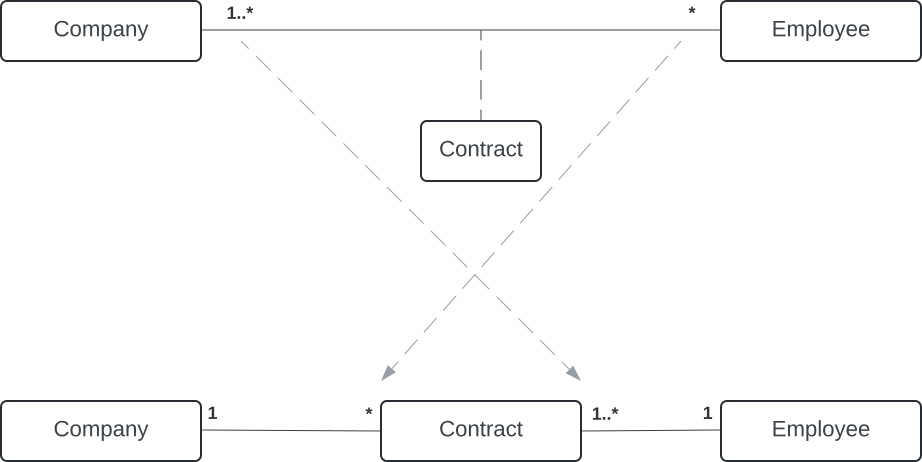
\includegraphics[scale=0.4]{part three/Klassendiagramme - Erweiterte Konzepte und Paketdiagramme/img/assoziationsklasse}
    \caption{Darstellung einer Assoziation mit Hilfe einer Assoziationsklasse (oben) sowie Transformation in gewöhnliche Assoziationen (unten). (Quelle: in Anlehnung an \cite[279, Abb. 4.4-11]{Oes05})}
    \label{fig:assoziationsklasse-cc}
\end{figure}

\clearpage


\section{Sequenzdiagramme}

\begin{tcolorbox}[title=Sequenzdiagramme]
    \textbf{Sequenzdiagramme} stellen Verhalten auf der Ebene einer Interaktion dar.\\
    In der Phase des Klassendesigns werden die Teilnehmer der Interaktionen bestimmt, weshalb Sequenzdiagramme oft in dieser Phase genutzt werden.\\
    In der \textbf{Analysephase} können Sequenzdiagramme eingesetzt werden, um die Kommunikation der bis dahin ausgemachten \textbf{Geschäftsobjekte} zu modellieren, oder um \textbf{Anwendungsfälle} weiter zu spezifizieren.
\end{tcolorbox}
\clearpage

\section{Aggregation}

\begin{tcolorbox}[title=Aggregation]
    Eine \textbf{Aggregation} ist in ihrer \semantischen Aussage unscharf (vgl.~\cite[40]{Buh09}).\\
    Sie beschreibt eine \textit{Ganzes}-\textit{Teile}-Beziehung, aber die \textit{Teile} können zu mehreren verschiedenen \textit{Ganzen} gehören.\\
    Außerdem kann ein Teil dem \textit{Ganzen} jederzeit wieder entnommen werden und das \textit{Ganze} ist nicht verantwortlich für das Erstellen der \textit{Teile}, weshalb Implementierungen beim Hinzufügen von Teilen oft schon fertige Objekte erwarten, die jeweils eines der \textit{Teile} repräsentieren.\\
    Aggregationsbeziehungen werden durch eine nicht-gefüllte Raute an der Seite der Klasse, die das Ganze repräsentiert, dargestellt.
\end{tcolorbox}
\clearpage

\section{Komposition}

\begin{tcolorbox}[title=Komposition]
    Bei einer \textbf{Komposition} handelt es sich um eine \textit{Ganzes}-\textit{Teile}-Beziehung, bei der das \textit{Ganze} verantwortlich für die Erstellung und Beseitigung der \textit{Teile} ist.
    Außerdem sind die \textit{Teile} an die \textbf{Existenz} des \textit{Ganzen} gebunden.\\
    \textit{Teile} gehören immer zu \textit{genau einem} \textit{Ganzen}.\\
    Eine Komposition wird dargestellt durch eine gefüllte Raute an der Klassenbox, die das \textit{Ganze} repräsentiert.
\end{tcolorbox}
\clearpage

\section{Paketdiagramm}

\begin{tcolorbox}[title=Komposition]
    \textbf{Paketdiagramme} zeigen Pakete und ihre Abhängigkeiten und werden in frühen Designphasen genutzt, um Strukturen (großer Systeme) aufzuzeigen.\\

    \noindent
    Elemente sollten so in Paketen gruppiert werden, dass ihr \textbf{funktionaler Zusammenhalt} (\textit{Kohäsion}, s. Abschnitt~\ref{subsec:hohe-kohasion}) klar wird.\\
    Hierdurch kann vermieden werden, dass Änderungen einer Klasse eines Paketes auch Änderungen außerhalb des Paketes erfordern.\\
    Außerdem erhöht sich die Wahrscheinlichkeit, dass einzelne Pakete als solche in anderen Projekten wiederverwendet werden können.\\

    \noindent
    In Paketdiagrammen können Beziehungen über folgende Schlüsselwörter deutlich gemacht werden:

    \begin{itemize}
        \item \guillemotleft import\guillemotright
        \item[] $\rightarrow$ \textbf{public-Import} zwischen Quell- und Zielpaket; Quellpaket kann die öffentlichen Elemente des Zielpaketes unter Verwendung des unqualifizierten und des qualifizierten Namens verwenden; die importierten Elemente sind auch für Pakete sichtbar, die das Quellpaket importieren
        \item \guillemotleft access\guillemotright
        \item[] $\rightarrow$ \textbf{privater Import} zwischen Quell- und Zielpaket; Zugriff auf Elemente des importierten Paketes ohne qualifizierenden Namen möglich; der Import eines Paketes in \textbf{Java} entspricht der \guillemotleft access\guillemotright-Beziehung
        \item \guillemotleft merge\guillemotright
        \item[] $\rightarrow$ Bei einem \textbf{merge} werden Elemente eines Zielpaketes in das Quellpaket
   \end{itemize}
\end{tcolorbox}
\clearpage

\section{Anwendungsfalldiagramm}

\begin{tcolorbox}[title=Anwendungsfalldiagramm]
    Die \textbf{Anwendungsfallanalyse} wird im Rahmen der \textbf{Anforderungsspezifikation} eingesetzt.\\

    \noindent
    Anwendungsfalldiagramme sind das am häufigsten eingesetzte Mittel zur Aufnahme und Darstellung von \textbf{Anforderungen}.\\
    Sie beschreiben selbst kein Verhalten und keine Abläufe, sondern zeigen nur die Zusammenhänge der an Anwendungsfällen beteiligten Modellelemente und sind somit ein Hilfsmittel zur Anforderungsermittlung und Verwaltung.\\

    \noindent
    Zu den wichtigsten Schritten einer Anwendungsfallanalyse gehören:
    \begin{enumerate}
        \item Akteure identifizieren
        \item Anwendungsfälle identifizieren
        \item Beschreiben der Akteure und Anwendungsfälle
        \item Identifizieren von \textit{Schlüsselobjekten}, die das System verwaltet
        \item Identifizieren der wichtigsten Anwendungsfälle (Priorisierung)
        \item detailliertere Beschreibung der Anwendungsfälle
        \item Strukturierung des Anwendungsfalldiagramms
    \end{enumerate}

    \noindent
    Anwendungsfälle beschreiben das \textbf{Szenario} der Nutzung, und nicht Features des Systems.
\end{tcolorbox}

\clearpage

\input{chapters/Anhang/CheatSheets/SE3/Aktivitätsdiagramm}
\clearpage

\section{Zustandsautomat}

\begin{tcolorbox}[title=Zustandsautomat]
    Mit \textbf{Zustandsautomaten} kann das \textit{Verhalten} von Systemen modelliert werden, wobei die \textit{Reaktionen} des Systems im Mittelpunkt stehen, und nicht die \textit{Aktionen}, wie bspw. bei den \textbf{Aktivitätsdiagrammen}.\\

    \noindent
        Ein \textbf{Zustandsautomat} kann den \textit{Lebensweg} eines Objektes modellieren, weshalb Zustandsautomaten oft im \textbf{Entwurf} als Ergänzung zu den \textbf{Klassendiagrammen} eingesetzt werden.
\end{tcolorbox}

\begin{figure}
    \centering
    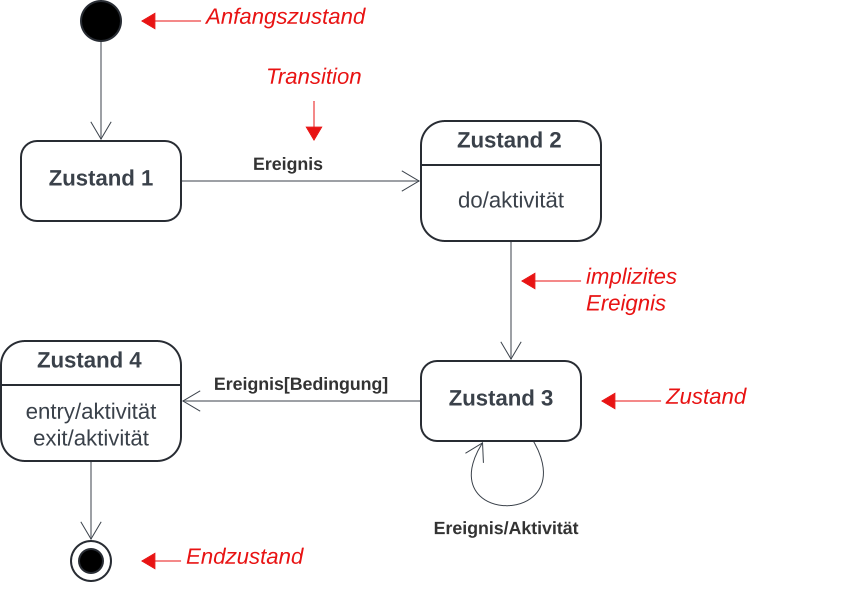
\includegraphics[scale=0.4]{part three/Zustandsautomaten/img/statechartdiagramnotation}
    \caption{Elemente eines einfachen Zustandsautomaten. Eine Transitionen wird durch ein \textbf{Ereignis} ausgelöst, das ein \textit{Signal}, ein \textit{Operationsaufruf} oder auch eine bestimmte \textit{Attributänderung} sein kann. (Quelle: in Anlehnung an \cite[90, Abb. 2.11-6]{Bal05})}
    \label{fig:statechartdiagramnotation-cc}
\end{figure}

\begin{minted}[fontsize=\small]{java}
// Beispiel für eine Implementierung eines
// Parkscheinautomaten als Zustandsautomat in Java
class Parkscheinautomat {

  // zustände
  private final int BEREIT = 0;
  private final int ZAHLUNG = 1;
  private final int ABBRUCH = 2;
  private final int BELEG   = 3;

  // Zustand; wird initial beim Starten
  // des Automaten gesetzt
  private int zustand;

  // Methoden lösen Aktionen beim Eintritt
  // in die jeweiligen Zustände aus
  private int zahlung() {
    // verarbeiten
    // danach neuen Zustand zurückliefern...
    ...
    return BEREIT;
  }

   ...

  private void bereit() {
    while (true) {
      // eingabe überprüfen und
      // ggf. Zustandswechsel auslösen:
      // Zustand als Attribut setzen
      ...
    }
  }

  public void start() {
    zustand = BEREIT;

    while(true) {
      switch (zustand) {
        case BEREIT:
          zustand = bereit();
        // ... weiteres Verhalten
        ...
      }
    }
  }
}
\end{minted}
\clearpage
	

\section{Inhalt SE3}

\section*{1. Übersicht UML}

\subsection*{Lernziele}
\begin{itemize}
    \item einen Einblick in den Sprachaufbau der UML 2.0 gewinnen
    \item einen Überblick über die Diagramme der UML 2.0 und deren Zweck haben
\end{itemize}

\subsection*{Zusammenfassung}
\begin{itemize}
    \item Die \textbf{UML} ist eine weit verbreitete Modellierungssprache zur Modellierung objektorientierter Softwaresysteme.
    \item Die UML 2.0 Spezifikation besteht aus vier Teilen:
    \begin{enumerate}
        \item \textbf{Superstructure}: Diagrammtypen
        \item \textbf{Infrastructure}: Modellierungskonzepte
        \item \textbf{OCL}: formale Sprache zur Formulierung von Einschränkungen
        \item \textbf{Diagram Interchange}: Austauschformate
    \end{enumerate}
    \item Die UML kann im \textbf{Sketching} oder \textbf{Blueprint Modus} eingesetzt werden, oder als Grundlage für \textbf{automatische Codegenerierung}
    \item Die UML ist an keinen speziellen Entwicklungsprozess gebunden
\end{itemize}

\section*{2. Klassendiagramme}

\subsection*{Lernziele}
\begin{itemize}
    \item wissen, wie Klassendiagramme im Entwicklungsprozess eingesetzt werden
    \item Klassendiagramme für Analyse- und Designentscheidungen einsetzen können
    \item die wichtigsten Modellierungskonzepte kennen
    \item sinnvolle Klassendiagramme erstellen und Java-Implementierungen ableiten können
    \item Klassendiagramme aus Java Quellcode erzeugen können
\end{itemize}

\subsection*{Zusammenfassung}

\begin{itemize}
    \item \textbf{Klassendiagramme} dienen zur \textbf{strukturellen Darstellung} von Softwaresystemen
    \item hierbei werden Klassen und \textbf{Beziehungen} zwischen Klassen dargestellt
    \item Properties können durch die \textbf{Attribut}- oder \textbf{Assoziationsnotation} modelliert werden
    \item Operationen werden als separate Zeile in ihrem Compartment dargestellt
    \item im Klassendiagramm können auch \textbf{Generalisierungsbeziehungen} modelliert werden
    \item \textbf{Abhängigkeitsbeziehungen} drücken ein Verhältnis zwischen \textbf{Client} und \textbf{Supplier} aus
\end{itemize}

\section*{3. Objektorientierter Entwurf}

\subsection*{Lernziele}
\begin{itemize}
    \item das Wesen einer Interaktion kennen
    \item wissen, wie Sequenzdiagramme im Entwicklungsprozess eingesetzt werden
    \item Sequenzdiagramme für Analyse- und Designentscheidungen sowie zur Darstellung von Kontrollflüssen einsetzen können
    \item die wichtigsten Modellierungskonzepte kennen
    \item sinnvolle Sequenzdiagramme erstellen und Java-Implementierungen ableiten können
    \item Sequenzdiagramme aus Java Quellcode erzeugen können
\end{itemize}

\subsection*{Zusammenfassung}

\begin{itemize}
    \item Sequenzdiagramme sind \textbf{Verhaltensdiagramme}
    und können im gesamten Entwicklungszyklus zur Modellierung von Interaktionen angewendet werden
    \item Interaktionen bestehen im Wesentlichen aus dem Nachrichtenaustausch zwischen verschiedenen Kommunikationspartnern
    \item in den meisten Fällen wird die Kommunikation von Objekten von Klassen modelliert, aber es können auch Teilnehmer auf anderen Ebenen modelliert werden
    \item gewöhnlich gibt ein Sequenzdiagramm einen \textbf{Anwendungsfall} (\textit{Szenario}) wieder
    \item sie dienen nicht dazu, um Zustandsänderungen darzustellen (hierfür werden Zustandsdiagramme verwendet)
    \item Sequenzdiagramme sind \textit{nicht} gut geeignet für die Darstellung von
    \begin{itemize}
        \item nebenläufigem Verhalten (\textit{asynchrone} Nachrichten, \textit{kombiniertes Fragment})
        \item Schleifen und alternativem Verhalten (\textit{kombinierte Fragmente})
        \item[] $\rightarrow$  für beide Fälle sind \textbf{Aktivitätsdiagramme} besser geeignet
    \end{itemize}
\end{itemize}

\section*{4. Klassendiagramme - Erweiterte Konzepte und Paketdiagramme}

\subsection*{Lernziele}
\begin{itemize}
    \item erweiterte Modellierungskonzepte in Klassendiagrammen für den Detailentwurf von Systemen kennen
    \item die Konsequenzen dieser Konzepte in der Implementierung kennen
    \item wissen, wie Paketdiagramme im Entwicklungsprozess eingesetzt werden
    \item die Modellierungskonzepte in Paketdiagrammen kennen
    \item anhand von Paketdiagrammen Software-Architekturen gestalten und bewerten können
\end{itemize}

\subsection*{Zusammenfassung}

\begin{itemize}
    \item Die vorgestellten erweiterten Konzepte werden vor allem im \textbf{Feinentwurf} von Klassenstrukturen eingesetzt.
    \item Generell gilt, dass die Spezifikationen von Objekten und Properties nur so detailliert ausgeführt werden sollen, wie nötig: Sind Details für das Verständnis unnötig, sollte darauf verzichtet werden.
    \item \textbf{Generalisierungsbeziehungen} sollten grundsätzlich modelliert werden.
    \item Ist eine \textbf{Komposition} statt einer Generalisierung für den Sachverhalt möglich, sollte diese verwendet werden: ``Favor object composition over inheritance.`` (\cite[19 f.]{GHJV94})
    \item \textbf{Kompositionsbeziehungen} geben eindeutige Impulse für eine Implementierung, \textbf{Aggregationsbeziehungen} sind in ihrer semantischen Aussage nicht sehr eindeutig
    \item \textbf{Assoziationsklassen} sind in ihrer frühen Designphase empfehlenswert, die Realisierung (mit {bspw.} Java) erfordert aber eine Transformation in eine volle Klasse, wobei die Multiplizitäten angepasst werden müssen
    \item Elemente können in \textbf{Paketen} zusamengefasst und unter einem gemeinsamen Namensraum gruppiert werden
\end{itemize}

\section*{4. Anwendungsfalldiagramm (Use-Case-Diagramm)}

\subsection*{Lernziele}
\begin{itemize}
    \item wissen, wie die Anwendungsfallanalyse im Rahmen der Anforderungsspezifikation eingesetzt wird
    \item Prozessschritte der Anwendungsfallanalyse beherrschen
    \item die wichtigsten Modellierungskonzepte in Anwendungsfalldiagrammen kennen
    \item den Aufbau einer Anwendungsfallbeschreibung kennen
\end{itemize}

\subsection*{Zusammenfassung}

\begin{itemize}
    \item \textbf{Anwendungsfalldiagramme} besitzen eine einfache Notation, um \textbf{Akteure} und \textbf{Anwendungsfälle} eines \textbf{Systems} grafisch darzustellen
    \item auf Basis eines Anwendungsfalldiagramms lässt sich ermitteln, ob die Anwendungsfälle gewünschtes Verhalten realisieren bzw. Beziehungen zu einem oder mehreren Akteuren haben
    \item Anwendungsfälle und Akteure \textit{müssen} zusätzlich textlich beschrieben werden
\end{itemize}

\section*{5. Aktivitätsdiagramme}

\subsection*{Lernziele}
\begin{itemize}
    \item wissen, wie Aktivitätsdiagramme im Rahmen der Verhaltensanalyse in verschiedenen Prozessphasen eingesetzt werden können
    \item die wichtigsten Modellierungskonzepte in Aktivitätsdiagrammen kennen
    \item Aktivitätsdiagramme interpretieren, erstellen und implementieren können
\end{itemize}

\subsection*{Zusammenfassung}

\begin{itemize}
    \item \textbf{Aktivitätsdiagramme} gehören zu den \textbf{Verhaltensdiagrammen} und können im \textit{gesamten} \textbf{Entwicklungsprozess} eingesetzt werden
    \item durch ein Aktivitätsdiagramm kann gezeigt werden, wie \textbf{Verhalten} realisiert wird
    \item es können mehrere \textbf{Aktivitäten} dargestellt werden
    \item \textbf{Aktivitätskanten} und \textbf{Aktivitätsknoten} werden zur Beschreibung von Verhalten verwendet
\end{itemize}

\section*{5. Zustandsautomaten}

\subsection*{Lernziele}
\begin{itemize}
    \item wissen, wie Zustandsdiagramme im Rahmen der Verhaltensanalyse einzelner Objekte eingesetzt werden können
    \item die wichtigsten Modellierungskonzepte in Zustandsdiagrammen kennen
    \item Zustandsdiagramme interpretieren, erstellen und implementieren können
\end{itemize}

\subsection*{Zusammenfassung}

\begin{itemize}
    \item Das \textbf{Zustandsdiagramm} gehört wie das \textbf{Aktivitätsdiagramm} zu den \textbf{Verhaltensdiagrammen}.
    \item Ein Zustandsdiagramm zeigt den \textbf{Lebensweg} eines \textbf{Objektes}.
    \item \textbf{Attributwerte} bestimmen den Zustand eines Objektes.
    \item \textbf{Transitionen} zwischen Zuständen werden durch \textbf{Guards} und \textbf{Events} gesteuert.
    \item Während der Transitionen können \textbf{Effekte} (\textit{Aktivitäten}) realisiert werden.
    \item Die Modellierung \textbf{zusammengesetzter Zustände} ist ebenfalls möglich.
    \item Für die Darstellung \textbf{paralleler} oder  \textbf{konkurrierender} Abläufe können \textbf{Regionen} modelliert werden.
\end{itemize}
\clearpage


\section{UML Modellierung}

\begin{tcolorbox}[title=UML Modellierung]
    \textbf{Modelle} haben die Aufgabe, den Bezug zum Original (Programm, Softwaresystem) herzustellen, sowie zu der \textit{Anwendungsumgebung}.\\
    Ein \textbf{Modell} enthält alle \textbf{Modellelemente}, die zur Beschreibung eines Softwaresystems nötig sind.\\

    \noindent
    Ein \textbf{Modellelement} wird als Element in einem UML Modell von einem Benutzer erstellt und auf verschiedenen \textbf{Diagrammen} (Struktur-/Verhaltensdiagrammen) platziert, und wird durch die \textbf{UML Modellierungskonzepte} als Metaklasse des \textbf{Metamodells} der UML beschrieben: \textbf{Modellelemente} werden aus Modellierungskonzepten instanziiert.\\

    \noindent
       Das \textbf{UML Metamodell} regelt, in welchem Zusammenhang \textbf{UML Modellierungskonzepte} in Modellen auftreten dürfen, und welche Eigenschaften und Beziehungen zu anderen Sprachelementen zulässig sind.\\

       \noindent
       Die im \textbf{Metamodell} verwendeten Erklärungen basieren auf einer abstrakten Syntax, für deren Beschreibung eine Untermenge (\textit{Klassendiagramme}) der UML verwendet wird.\\
        Die \textbf{Semantik} der Modellierungskonzepte wird textlich beschrieben, zur Formalisierung von Regeln für die syntaktische Korrektheit wird die \textbf{OCL} (\textit{Object Constraint Language}) verwendet.
\end{tcolorbox}

\begin{figure}
    \centering
    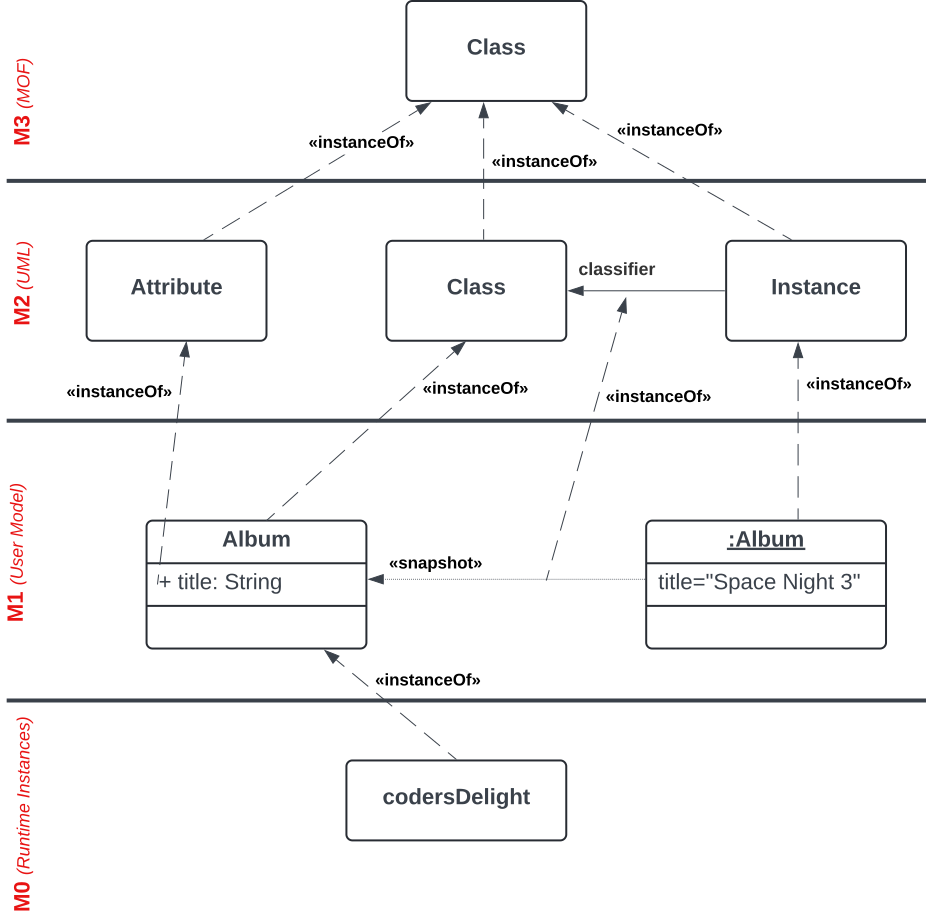
\includegraphics[scale=0.4]{part three/Einführung/img/metamodel}
    \caption{Beispiel für die verschiedenen Schichten der Metamodell Hierarchie.
        In der original Abbildung sind die Pfeilspitzen offen. (Quelle: in Anlehnung an S. 20, Figure 7.8, \url{https://www.omg.org/spec/UML/2.4.1/Infrastructure/PDF}, abgerufen 01.05.2024}
    \label{fig:metamodel-cc}
\end{figure}

\clearpage


\section{Strukturdiagramme}

\begin{tcolorbox}[title=Strukturdiagramme]
    In den \textbf{Strukturdiagrammen} werden \textbf{statische Strukturaspekte} eines Systems betrachtet.
    Für eine Systemmodellierung können alle dieser 6 Diagramme verwendet werden.

    \begin{itemize}
        \item \textbf{Klassendiagramm}: Das \textbf{Klassendiagramm} wird verwendet, um ein objektorientiertes System zu beschreiben.
        \item \textbf{Paketdiagramm}: Ein \textbf{Paketdiagramm} zeigt die Pakete eines Systems und deren Beziehungen.
        \item \textbf{Komponentendiagramm}: Stellt Komponenten oder auch \textit{Subsysteme} mit definierten Interfaces dar, um bspw. \textbf{Architekturdesign} darzustellen.
        \item \textbf{Verteilungsdiagramm}: Beschreibt eine Menge von Knoten, die die \textit{Ausführungsarchitektur} eines Systems definieren können, wobei Knoten i.d.R. \textit{Geräte} oder \textit{Softwareablaufumgebungen repräsentieren}.
        \item \textbf{Kompositionsstrukturdiagramm}: Stellt die \textbf{Komposition} von \textit{Systemstrukturen} (Klassen, Komponenten, Gesamtsystem) in einem bestimmten \textit{Kontext} mit einem bestimmten \textit{Ziel} dar (vgl. \cite[9]{Buh09}).
        \item \textbf{Objektdiagramm}: Momentaufnahme eines Systems zu genau einem \textit{Zeitpukt} während der Ausführung
    \end{itemize}

\end{tcolorbox}
\clearpage

\section{Verhaltensdiagramme}

\begin{tcolorbox}[title=Verhaltensdiagramme]
    \textbf{Verhaltensdiagramme} stellen \textit{Dynamik}, \textit{interne Abläufe} und das \textit{Zusammenspiel} der Systemteile dar, um eine Spezifikation zu vervollständigen.

    \begin{itemize}
        \item \textbf{Anwendungsfalldiagramm}: Dienen zur \textit{Spezifizierung} und \textit{Formalisierung} von \textit{Systemanforderungen}, unter Berücksichtigung von \textbf{Akteuren}, \textbf{Systemen} und \textbf{Anwendungsfällen}
        \item \textbf{Zustandsdiagramm}: Auch \textbf{Zustandsautomaten}; zeigen für ein einzelnes Objekt Zustandsänderungen während der Lebenszeit
        \item \textbf{Aktivitätsdiagramme}: Werden zur Modellierung von \textit{Kontroll}- oder \textit{Objektflüssen} oder zur Darstellung von \textit{Programmlogik} genutzt.
        \item \textbf{Interaktionsdiagramme}: Stellen das Zusammenspiel mehrerer Kommunikationspartner dar.
        Es gibt unterschiedliche Typen von Interaktionsdiagrammen, die Interaktionen auf verschiedenen \textit{Abstraktionsebenen} modellieren:
        \begin{itemize}
            \item \textbf{Sequenzdiagramm}: Zeigt den Verlauf einer Interaktion in zwei Dimensionen, \textit{Kommunikationspartner} und die Nachrichten in ihrer \textit{zeitlichen Abfolge}
            \item \textbf{Kommunikationsdiagramm}: hebt die Kommunikationsbeziehungen zwischen den Partnern hervor
            \item \textbf{Timing Diagramm}: hebt die zeitlichen Aspekte einer Interaktion hervor
            \item \textbf{Interaktionsüberblickdiagramm}: Spezialfall des \textbf{Aktivitätsdiagramms} - statt Aktionen und Aktivitäten können das \textbf{Sequenz}-, \textbf{Kommunikations}- und das \textbf{Timing}-Diagramm als Knoten verwendet werden.
        \end{itemize}
        Alle verwenden dieselben Grundelemente: \textit{Lebenslinien} der Akteure und Nachrichten, die zwischen diesen ausgetauscht werden.
    \end{itemize}
\end{tcolorbox}

\clearpage


\section{Klassendiagramm}

\begin{tcolorbox}[title=Klassendiagramm]
    Das \textbf{Klassendiagramm} beschreibt die Klassen eines Systems und die statischen Beziehungen zwischen ihnen.\\
    Sie werden in Form von Domainklassen bei der \textbf{Analyse} und als detaillierte Entwürfe von Systemklassen als \textit{Blueprint} im \textbf{gesamten Entwicklungsprozess} eingesetzt.

\end{tcolorbox}
\clearpage


\section{Assoziationsklasse (Attributierte Assoziation)}

\begin{tcolorbox}[title=Assoziationsklasse (Attributierte Assoziation)]
Eine \textbf{Assoziationsklasse} erlaubt das Hinzufügen von Operationen und Attributen zu einer Assoziation (\cite[43]{Buh09}).\\
Assoziationsklassen werden in der \textbf{Analyse} in Modellen verwendet und in dem \textbf{Entwurf} in eigenständige Klassen transformiert.\\

\noindent
Assoziationsklassen werden in der \textbf{Analyse} in Modellen verwendet und in dem \textbf{Entwurf} in eigenständige Klassen transformiert.

\blockquote[{\cite[277]{Oes05}}]{
    Eine attributierte Assoziation ist immer dann nahe liegend, wenn Attribute oder Operationen gefunden werden, die weder der einen noch der anderen Klasse zugeordnet werden können, weil sie nämlich Eigenschaften der Beziehung selbst sind.
}.\\

Bei einer attributierten Assoziation dürfen zwei beteiligte Objekte maximal nur eine Beziehung zueinander haben (vgl.~\cite[277]{Oes05})\footnote{
    \textit{Ostereich} führt dies ebenda auf Seite 278 weiter aus, in dem er beschreibt, wie eine attributierte Assoziation für ein \textit{Beschäftigtenverhältnis} zwischen \textit{Mitarbeiter} und \textit{Unternehmen} modelliert wird. Dabei wird davon ausgegangen, dass ein \textit{Mitarbeiter} nur über \textit{ein} Arbeitsverhältnis mit einem \textit{Unternehmen} in Beziehung stehen kann. Bestehen mehrere Arbeitsverhältnisse (\textit{Mitarbeiter} hat zu unterschiedlichen Zeitpunkten für das \textit{Unternehmen} gearbeitet), kann die attributierte Assoziation nicht verwendet werden.\\

\noindent
Wird eine attributierte Assoziation in eine gewöhnliche Assoziation transformiert, muss darauf geachtet werden, die Multiplizitäten richtig zu setzen (s. Abbildung~\ref{fig:assoziationsklasse}).
\end{tcolorbox}

\begin{figure}
    \centering
    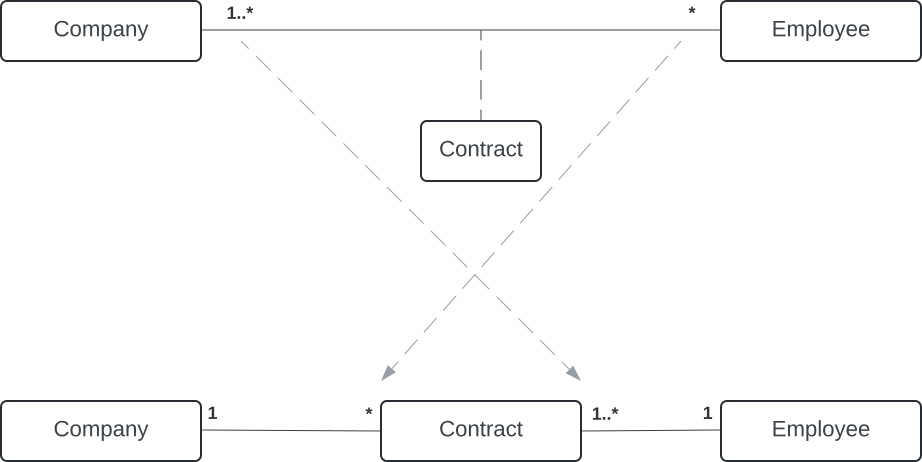
\includegraphics[scale=0.4]{part three/Klassendiagramme - Erweiterte Konzepte und Paketdiagramme/img/assoziationsklasse}
    \caption{Darstellung einer Assoziation mit Hilfe einer Assoziationsklasse (oben) sowie Transformation in gewöhnliche Assoziationen (unten). (Quelle: in Anlehnung an \cite[279, Abb. 4.4-11]{Oes05})}
    \label{fig:assoziationsklasse-cc}
\end{figure}

\clearpage


\section{Sequenzdiagramme}

\begin{tcolorbox}[title=Sequenzdiagramme]
    \textbf{Sequenzdiagramme} stellen Verhalten auf der Ebene einer Interaktion dar.\\
    In der Phase des Klassendesigns werden die Teilnehmer der Interaktionen bestimmt, weshalb Sequenzdiagramme oft in dieser Phase genutzt werden.\\
    In der \textbf{Analysephase} können Sequenzdiagramme eingesetzt werden, um die Kommunikation der bis dahin ausgemachten \textbf{Geschäftsobjekte} zu modellieren, oder um \textbf{Anwendungsfälle} weiter zu spezifizieren.
\end{tcolorbox}
\clearpage

\section{Aggregation}

\begin{tcolorbox}[title=Aggregation]
    Eine \textbf{Aggregation} ist in ihrer \semantischen Aussage unscharf (vgl.~\cite[40]{Buh09}).\\
    Sie beschreibt eine \textit{Ganzes}-\textit{Teile}-Beziehung, aber die \textit{Teile} können zu mehreren verschiedenen \textit{Ganzen} gehören.\\
    Außerdem kann ein Teil dem \textit{Ganzen} jederzeit wieder entnommen werden und das \textit{Ganze} ist nicht verantwortlich für das Erstellen der \textit{Teile}, weshalb Implementierungen beim Hinzufügen von Teilen oft schon fertige Objekte erwarten, die jeweils eines der \textit{Teile} repräsentieren.\\
    Aggregationsbeziehungen werden durch eine nicht-gefüllte Raute an der Seite der Klasse, die das Ganze repräsentiert, dargestellt.
\end{tcolorbox}
\clearpage

\section{Komposition}

\begin{tcolorbox}[title=Komposition]
    Bei einer \textbf{Komposition} handelt es sich um eine \textit{Ganzes}-\textit{Teile}-Beziehung, bei der das \textit{Ganze} verantwortlich für die Erstellung und Beseitigung der \textit{Teile} ist.
    Außerdem sind die \textit{Teile} an die \textbf{Existenz} des \textit{Ganzen} gebunden.\\
    \textit{Teile} gehören immer zu \textit{genau einem} \textit{Ganzen}.\\
    Eine Komposition wird dargestellt durch eine gefüllte Raute an der Klassenbox, die das \textit{Ganze} repräsentiert.
\end{tcolorbox}
\clearpage

\section{Paketdiagramm}

\begin{tcolorbox}[title=Komposition]
    \textbf{Paketdiagramme} zeigen Pakete und ihre Abhängigkeiten und werden in frühen Designphasen genutzt, um Strukturen (großer Systeme) aufzuzeigen.\\

    \noindent
    Elemente sollten so in Paketen gruppiert werden, dass ihr \textbf{funktionaler Zusammenhalt} (\textit{Kohäsion}, s. Abschnitt~\ref{subsec:hohe-kohasion}) klar wird.\\
    Hierdurch kann vermieden werden, dass Änderungen einer Klasse eines Paketes auch Änderungen außerhalb des Paketes erfordern.\\
    Außerdem erhöht sich die Wahrscheinlichkeit, dass einzelne Pakete als solche in anderen Projekten wiederverwendet werden können.\\

    \noindent
    In Paketdiagrammen können Beziehungen über folgende Schlüsselwörter deutlich gemacht werden:

    \begin{itemize}
        \item \guillemotleft import\guillemotright
        \item[] $\rightarrow$ \textbf{public-Import} zwischen Quell- und Zielpaket; Quellpaket kann die öffentlichen Elemente des Zielpaketes unter Verwendung des unqualifizierten und des qualifizierten Namens verwenden; die importierten Elemente sind auch für Pakete sichtbar, die das Quellpaket importieren
        \item \guillemotleft access\guillemotright
        \item[] $\rightarrow$ \textbf{privater Import} zwischen Quell- und Zielpaket; Zugriff auf Elemente des importierten Paketes ohne qualifizierenden Namen möglich; der Import eines Paketes in \textbf{Java} entspricht der \guillemotleft access\guillemotright-Beziehung
        \item \guillemotleft merge\guillemotright
        \item[] $\rightarrow$ Bei einem \textbf{merge} werden Elemente eines Zielpaketes in das Quellpaket
   \end{itemize}
\end{tcolorbox}
\clearpage

\section{Anwendungsfalldiagramm}

\begin{tcolorbox}[title=Anwendungsfalldiagramm]
    Die \textbf{Anwendungsfallanalyse} wird im Rahmen der \textbf{Anforderungsspezifikation} eingesetzt.\\

    \noindent
    Anwendungsfalldiagramme sind das am häufigsten eingesetzte Mittel zur Aufnahme und Darstellung von \textbf{Anforderungen}.\\
    Sie beschreiben selbst kein Verhalten und keine Abläufe, sondern zeigen nur die Zusammenhänge der an Anwendungsfällen beteiligten Modellelemente und sind somit ein Hilfsmittel zur Anforderungsermittlung und Verwaltung.\\

    \noindent
    Zu den wichtigsten Schritten einer Anwendungsfallanalyse gehören:
    \begin{enumerate}
        \item Akteure identifizieren
        \item Anwendungsfälle identifizieren
        \item Beschreiben der Akteure und Anwendungsfälle
        \item Identifizieren von \textit{Schlüsselobjekten}, die das System verwaltet
        \item Identifizieren der wichtigsten Anwendungsfälle (Priorisierung)
        \item detailliertere Beschreibung der Anwendungsfälle
        \item Strukturierung des Anwendungsfalldiagramms
    \end{enumerate}

    \noindent
    Anwendungsfälle beschreiben das \textbf{Szenario} der Nutzung, und nicht Features des Systems.
\end{tcolorbox}

\clearpage

\input{chapters/Anhang/CheatSheets/SE3/Aktivitätsdiagramm}
\clearpage

\section{Zustandsautomat}

\begin{tcolorbox}[title=Zustandsautomat]
    Mit \textbf{Zustandsautomaten} kann das \textit{Verhalten} von Systemen modelliert werden, wobei die \textit{Reaktionen} des Systems im Mittelpunkt stehen, und nicht die \textit{Aktionen}, wie bspw. bei den \textbf{Aktivitätsdiagrammen}.\\

    \noindent
        Ein \textbf{Zustandsautomat} kann den \textit{Lebensweg} eines Objektes modellieren, weshalb Zustandsautomaten oft im \textbf{Entwurf} als Ergänzung zu den \textbf{Klassendiagrammen} eingesetzt werden.
\end{tcolorbox}

\begin{figure}
    \centering
    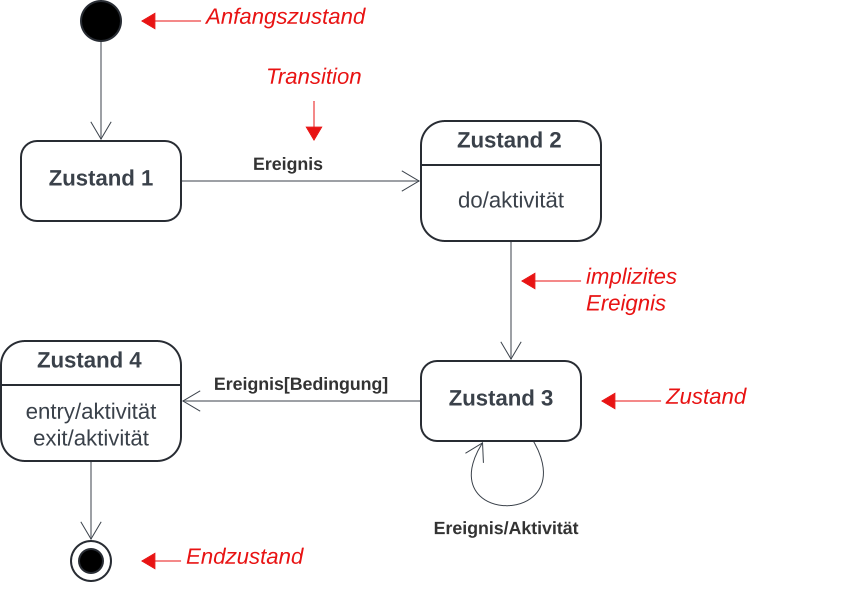
\includegraphics[scale=0.4]{part three/Zustandsautomaten/img/statechartdiagramnotation}
    \caption{Elemente eines einfachen Zustandsautomaten. Eine Transitionen wird durch ein \textbf{Ereignis} ausgelöst, das ein \textit{Signal}, ein \textit{Operationsaufruf} oder auch eine bestimmte \textit{Attributänderung} sein kann. (Quelle: in Anlehnung an \cite[90, Abb. 2.11-6]{Bal05})}
    \label{fig:statechartdiagramnotation-cc}
\end{figure}

\begin{minted}[fontsize=\small]{java}
// Beispiel für eine Implementierung eines
// Parkscheinautomaten als Zustandsautomat in Java
class Parkscheinautomat {

  // zustände
  private final int BEREIT = 0;
  private final int ZAHLUNG = 1;
  private final int ABBRUCH = 2;
  private final int BELEG   = 3;

  // Zustand; wird initial beim Starten
  // des Automaten gesetzt
  private int zustand;

  // Methoden lösen Aktionen beim Eintritt
  // in die jeweiligen Zustände aus
  private int zahlung() {
    // verarbeiten
    // danach neuen Zustand zurückliefern...
    ...
    return BEREIT;
  }

   ...

  private void bereit() {
    while (true) {
      // eingabe überprüfen und
      // ggf. Zustandswechsel auslösen:
      // Zustand als Attribut setzen
      ...
    }
  }

  public void start() {
    zustand = BEREIT;

    while(true) {
      switch (zustand) {
        case BEREIT:
          zustand = bereit();
        // ... weiteres Verhalten
        ...
      }
    }
  }
}
\end{minted}
\clearpage
	

\section{Inhalt SE3}

\section*{1. Übersicht UML}

\subsection*{Lernziele}
\begin{itemize}
    \item einen Einblick in den Sprachaufbau der UML 2.0 gewinnen
    \item einen Überblick über die Diagramme der UML 2.0 und deren Zweck haben
\end{itemize}

\subsection*{Zusammenfassung}
\begin{itemize}
    \item Die \textbf{UML} ist eine weit verbreitete Modellierungssprache zur Modellierung objektorientierter Softwaresysteme.
    \item Die UML 2.0 Spezifikation besteht aus vier Teilen:
    \begin{enumerate}
        \item \textbf{Superstructure}: Diagrammtypen
        \item \textbf{Infrastructure}: Modellierungskonzepte
        \item \textbf{OCL}: formale Sprache zur Formulierung von Einschränkungen
        \item \textbf{Diagram Interchange}: Austauschformate
    \end{enumerate}
    \item Die UML kann im \textbf{Sketching} oder \textbf{Blueprint Modus} eingesetzt werden, oder als Grundlage für \textbf{automatische Codegenerierung}
    \item Die UML ist an keinen speziellen Entwicklungsprozess gebunden
\end{itemize}

\section*{2. Klassendiagramme}

\subsection*{Lernziele}
\begin{itemize}
    \item wissen, wie Klassendiagramme im Entwicklungsprozess eingesetzt werden
    \item Klassendiagramme für Analyse- und Designentscheidungen einsetzen können
    \item die wichtigsten Modellierungskonzepte kennen
    \item sinnvolle Klassendiagramme erstellen und Java-Implementierungen ableiten können
    \item Klassendiagramme aus Java Quellcode erzeugen können
\end{itemize}

\subsection*{Zusammenfassung}

\begin{itemize}
    \item \textbf{Klassendiagramme} dienen zur \textbf{strukturellen Darstellung} von Softwaresystemen
    \item hierbei werden Klassen und \textbf{Beziehungen} zwischen Klassen dargestellt
    \item Properties können durch die \textbf{Attribut}- oder \textbf{Assoziationsnotation} modelliert werden
    \item Operationen werden als separate Zeile in ihrem Compartment dargestellt
    \item im Klassendiagramm können auch \textbf{Generalisierungsbeziehungen} modelliert werden
    \item \textbf{Abhängigkeitsbeziehungen} drücken ein Verhältnis zwischen \textbf{Client} und \textbf{Supplier} aus
\end{itemize}

\section*{3. Objektorientierter Entwurf}

\subsection*{Lernziele}
\begin{itemize}
    \item das Wesen einer Interaktion kennen
    \item wissen, wie Sequenzdiagramme im Entwicklungsprozess eingesetzt werden
    \item Sequenzdiagramme für Analyse- und Designentscheidungen sowie zur Darstellung von Kontrollflüssen einsetzen können
    \item die wichtigsten Modellierungskonzepte kennen
    \item sinnvolle Sequenzdiagramme erstellen und Java-Implementierungen ableiten können
    \item Sequenzdiagramme aus Java Quellcode erzeugen können
\end{itemize}

\subsection*{Zusammenfassung}

\begin{itemize}
    \item Sequenzdiagramme sind \textbf{Verhaltensdiagramme}
    und können im gesamten Entwicklungszyklus zur Modellierung von Interaktionen angewendet werden
    \item Interaktionen bestehen im Wesentlichen aus dem Nachrichtenaustausch zwischen verschiedenen Kommunikationspartnern
    \item in den meisten Fällen wird die Kommunikation von Objekten von Klassen modelliert, aber es können auch Teilnehmer auf anderen Ebenen modelliert werden
    \item gewöhnlich gibt ein Sequenzdiagramm einen \textbf{Anwendungsfall} (\textit{Szenario}) wieder
    \item sie dienen nicht dazu, um Zustandsänderungen darzustellen (hierfür werden Zustandsdiagramme verwendet)
    \item Sequenzdiagramme sind \textit{nicht} gut geeignet für die Darstellung von
    \begin{itemize}
        \item nebenläufigem Verhalten (\textit{asynchrone} Nachrichten, \textit{kombiniertes Fragment})
        \item Schleifen und alternativem Verhalten (\textit{kombinierte Fragmente})
        \item[] $\rightarrow$  für beide Fälle sind \textbf{Aktivitätsdiagramme} besser geeignet
    \end{itemize}
\end{itemize}

\section*{4. Klassendiagramme - Erweiterte Konzepte und Paketdiagramme}

\subsection*{Lernziele}
\begin{itemize}
    \item erweiterte Modellierungskonzepte in Klassendiagrammen für den Detailentwurf von Systemen kennen
    \item die Konsequenzen dieser Konzepte in der Implementierung kennen
    \item wissen, wie Paketdiagramme im Entwicklungsprozess eingesetzt werden
    \item die Modellierungskonzepte in Paketdiagrammen kennen
    \item anhand von Paketdiagrammen Software-Architekturen gestalten und bewerten können
\end{itemize}

\subsection*{Zusammenfassung}

\begin{itemize}
    \item Die vorgestellten erweiterten Konzepte werden vor allem im \textbf{Feinentwurf} von Klassenstrukturen eingesetzt.
    \item Generell gilt, dass die Spezifikationen von Objekten und Properties nur so detailliert ausgeführt werden sollen, wie nötig: Sind Details für das Verständnis unnötig, sollte darauf verzichtet werden.
    \item \textbf{Generalisierungsbeziehungen} sollten grundsätzlich modelliert werden.
    \item Ist eine \textbf{Komposition} statt einer Generalisierung für den Sachverhalt möglich, sollte diese verwendet werden: ``Favor object composition over inheritance.`` (\cite[19 f.]{GHJV94})
    \item \textbf{Kompositionsbeziehungen} geben eindeutige Impulse für eine Implementierung, \textbf{Aggregationsbeziehungen} sind in ihrer semantischen Aussage nicht sehr eindeutig
    \item \textbf{Assoziationsklassen} sind in ihrer frühen Designphase empfehlenswert, die Realisierung (mit {bspw.} Java) erfordert aber eine Transformation in eine volle Klasse, wobei die Multiplizitäten angepasst werden müssen
    \item Elemente können in \textbf{Paketen} zusamengefasst und unter einem gemeinsamen Namensraum gruppiert werden
\end{itemize}

\section*{4. Anwendungsfalldiagramm (Use-Case-Diagramm)}

\subsection*{Lernziele}
\begin{itemize}
    \item wissen, wie die Anwendungsfallanalyse im Rahmen der Anforderungsspezifikation eingesetzt wird
    \item Prozessschritte der Anwendungsfallanalyse beherrschen
    \item die wichtigsten Modellierungskonzepte in Anwendungsfalldiagrammen kennen
    \item den Aufbau einer Anwendungsfallbeschreibung kennen
\end{itemize}

\subsection*{Zusammenfassung}

\begin{itemize}
    \item \textbf{Anwendungsfalldiagramme} besitzen eine einfache Notation, um \textbf{Akteure} und \textbf{Anwendungsfälle} eines \textbf{Systems} grafisch darzustellen
    \item auf Basis eines Anwendungsfalldiagramms lässt sich ermitteln, ob die Anwendungsfälle gewünschtes Verhalten realisieren bzw. Beziehungen zu einem oder mehreren Akteuren haben
    \item Anwendungsfälle und Akteure \textit{müssen} zusätzlich textlich beschrieben werden
\end{itemize}

\section*{5. Aktivitätsdiagramme}

\subsection*{Lernziele}
\begin{itemize}
    \item wissen, wie Aktivitätsdiagramme im Rahmen der Verhaltensanalyse in verschiedenen Prozessphasen eingesetzt werden können
    \item die wichtigsten Modellierungskonzepte in Aktivitätsdiagrammen kennen
    \item Aktivitätsdiagramme interpretieren, erstellen und implementieren können
\end{itemize}

\subsection*{Zusammenfassung}

\begin{itemize}
    \item \textbf{Aktivitätsdiagramme} gehören zu den \textbf{Verhaltensdiagrammen} und können im \textit{gesamten} \textbf{Entwicklungsprozess} eingesetzt werden
    \item durch ein Aktivitätsdiagramm kann gezeigt werden, wie \textbf{Verhalten} realisiert wird
    \item es können mehrere \textbf{Aktivitäten} dargestellt werden
    \item \textbf{Aktivitätskanten} und \textbf{Aktivitätsknoten} werden zur Beschreibung von Verhalten verwendet
\end{itemize}

\section*{5. Zustandsautomaten}

\subsection*{Lernziele}
\begin{itemize}
    \item wissen, wie Zustandsdiagramme im Rahmen der Verhaltensanalyse einzelner Objekte eingesetzt werden können
    \item die wichtigsten Modellierungskonzepte in Zustandsdiagrammen kennen
    \item Zustandsdiagramme interpretieren, erstellen und implementieren können
\end{itemize}

\subsection*{Zusammenfassung}

\begin{itemize}
    \item Das \textbf{Zustandsdiagramm} gehört wie das \textbf{Aktivitätsdiagramm} zu den \textbf{Verhaltensdiagrammen}.
    \item Ein Zustandsdiagramm zeigt den \textbf{Lebensweg} eines \textbf{Objektes}.
    \item \textbf{Attributwerte} bestimmen den Zustand eines Objektes.
    \item \textbf{Transitionen} zwischen Zuständen werden durch \textbf{Guards} und \textbf{Events} gesteuert.
    \item Während der Transitionen können \textbf{Effekte} (\textit{Aktivitäten}) realisiert werden.
    \item Die Modellierung \textbf{zusammengesetzter Zustände} ist ebenfalls möglich.
    \item Für die Darstellung \textbf{paralleler} oder  \textbf{konkurrierender} Abläufe können \textbf{Regionen} modelliert werden.
\end{itemize}
\clearpage


\section{UML Modellierung}

\begin{tcolorbox}[title=UML Modellierung]
    \textbf{Modelle} haben die Aufgabe, den Bezug zum Original (Programm, Softwaresystem) herzustellen, sowie zu der \textit{Anwendungsumgebung}.\\
    Ein \textbf{Modell} enthält alle \textbf{Modellelemente}, die zur Beschreibung eines Softwaresystems nötig sind.\\

    \noindent
    Ein \textbf{Modellelement} wird als Element in einem UML Modell von einem Benutzer erstellt und auf verschiedenen \textbf{Diagrammen} (Struktur-/Verhaltensdiagrammen) platziert, und wird durch die \textbf{UML Modellierungskonzepte} als Metaklasse des \textbf{Metamodells} der UML beschrieben: \textbf{Modellelemente} werden aus Modellierungskonzepten instanziiert.\\

    \noindent
       Das \textbf{UML Metamodell} regelt, in welchem Zusammenhang \textbf{UML Modellierungskonzepte} in Modellen auftreten dürfen, und welche Eigenschaften und Beziehungen zu anderen Sprachelementen zulässig sind.\\

       \noindent
       Die im \textbf{Metamodell} verwendeten Erklärungen basieren auf einer abstrakten Syntax, für deren Beschreibung eine Untermenge (\textit{Klassendiagramme}) der UML verwendet wird.\\
        Die \textbf{Semantik} der Modellierungskonzepte wird textlich beschrieben, zur Formalisierung von Regeln für die syntaktische Korrektheit wird die \textbf{OCL} (\textit{Object Constraint Language}) verwendet.
\end{tcolorbox}

\begin{figure}
    \centering
    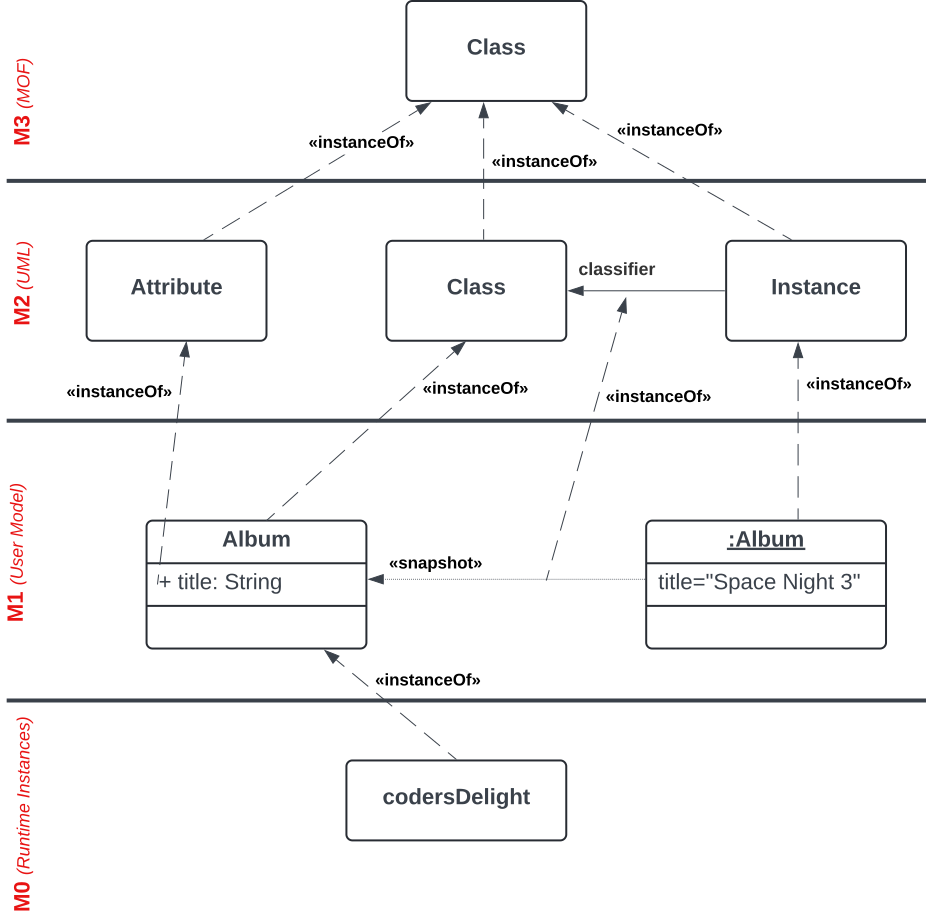
\includegraphics[scale=0.4]{part three/Einführung/img/metamodel}
    \caption{Beispiel für die verschiedenen Schichten der Metamodell Hierarchie.
        In der original Abbildung sind die Pfeilspitzen offen. (Quelle: in Anlehnung an S. 20, Figure 7.8, \url{https://www.omg.org/spec/UML/2.4.1/Infrastructure/PDF}, abgerufen 01.05.2024}
    \label{fig:metamodel-cc}
\end{figure}

\clearpage


\section{Strukturdiagramme}

\begin{tcolorbox}[title=Strukturdiagramme]
    In den \textbf{Strukturdiagrammen} werden \textbf{statische Strukturaspekte} eines Systems betrachtet.
    Für eine Systemmodellierung können alle dieser 6 Diagramme verwendet werden.

    \begin{itemize}
        \item \textbf{Klassendiagramm}: Das \textbf{Klassendiagramm} wird verwendet, um ein objektorientiertes System zu beschreiben.
        \item \textbf{Paketdiagramm}: Ein \textbf{Paketdiagramm} zeigt die Pakete eines Systems und deren Beziehungen.
        \item \textbf{Komponentendiagramm}: Stellt Komponenten oder auch \textit{Subsysteme} mit definierten Interfaces dar, um bspw. \textbf{Architekturdesign} darzustellen.
        \item \textbf{Verteilungsdiagramm}: Beschreibt eine Menge von Knoten, die die \textit{Ausführungsarchitektur} eines Systems definieren können, wobei Knoten i.d.R. \textit{Geräte} oder \textit{Softwareablaufumgebungen repräsentieren}.
        \item \textbf{Kompositionsstrukturdiagramm}: Stellt die \textbf{Komposition} von \textit{Systemstrukturen} (Klassen, Komponenten, Gesamtsystem) in einem bestimmten \textit{Kontext} mit einem bestimmten \textit{Ziel} dar (vgl. \cite[9]{Buh09}).
        \item \textbf{Objektdiagramm}: Momentaufnahme eines Systems zu genau einem \textit{Zeitpukt} während der Ausführung
    \end{itemize}

\end{tcolorbox}
\clearpage

\section{Verhaltensdiagramme}

\begin{tcolorbox}[title=Verhaltensdiagramme]
    \textbf{Verhaltensdiagramme} stellen \textit{Dynamik}, \textit{interne Abläufe} und das \textit{Zusammenspiel} der Systemteile dar, um eine Spezifikation zu vervollständigen.

    \begin{itemize}
        \item \textbf{Anwendungsfalldiagramm}: Dienen zur \textit{Spezifizierung} und \textit{Formalisierung} von \textit{Systemanforderungen}, unter Berücksichtigung von \textbf{Akteuren}, \textbf{Systemen} und \textbf{Anwendungsfällen}
        \item \textbf{Zustandsdiagramm}: Auch \textbf{Zustandsautomaten}; zeigen für ein einzelnes Objekt Zustandsänderungen während der Lebenszeit
        \item \textbf{Aktivitätsdiagramme}: Werden zur Modellierung von \textit{Kontroll}- oder \textit{Objektflüssen} oder zur Darstellung von \textit{Programmlogik} genutzt.
        \item \textbf{Interaktionsdiagramme}: Stellen das Zusammenspiel mehrerer Kommunikationspartner dar.
        Es gibt unterschiedliche Typen von Interaktionsdiagrammen, die Interaktionen auf verschiedenen \textit{Abstraktionsebenen} modellieren:
        \begin{itemize}
            \item \textbf{Sequenzdiagramm}: Zeigt den Verlauf einer Interaktion in zwei Dimensionen, \textit{Kommunikationspartner} und die Nachrichten in ihrer \textit{zeitlichen Abfolge}
            \item \textbf{Kommunikationsdiagramm}: hebt die Kommunikationsbeziehungen zwischen den Partnern hervor
            \item \textbf{Timing Diagramm}: hebt die zeitlichen Aspekte einer Interaktion hervor
            \item \textbf{Interaktionsüberblickdiagramm}: Spezialfall des \textbf{Aktivitätsdiagramms} - statt Aktionen und Aktivitäten können das \textbf{Sequenz}-, \textbf{Kommunikations}- und das \textbf{Timing}-Diagramm als Knoten verwendet werden.
        \end{itemize}
        Alle verwenden dieselben Grundelemente: \textit{Lebenslinien} der Akteure und Nachrichten, die zwischen diesen ausgetauscht werden.
    \end{itemize}
\end{tcolorbox}

\clearpage


\section{Klassendiagramm}

\begin{tcolorbox}[title=Klassendiagramm]
    Das \textbf{Klassendiagramm} beschreibt die Klassen eines Systems und die statischen Beziehungen zwischen ihnen.\\
    Sie werden in Form von Domainklassen bei der \textbf{Analyse} und als detaillierte Entwürfe von Systemklassen als \textit{Blueprint} im \textbf{gesamten Entwicklungsprozess} eingesetzt.

\end{tcolorbox}
\clearpage


\section{Assoziationsklasse (Attributierte Assoziation)}

\begin{tcolorbox}[title=Assoziationsklasse (Attributierte Assoziation)]
Eine \textbf{Assoziationsklasse} erlaubt das Hinzufügen von Operationen und Attributen zu einer Assoziation (\cite[43]{Buh09}).\\
Assoziationsklassen werden in der \textbf{Analyse} in Modellen verwendet und in dem \textbf{Entwurf} in eigenständige Klassen transformiert.\\

\noindent
Assoziationsklassen werden in der \textbf{Analyse} in Modellen verwendet und in dem \textbf{Entwurf} in eigenständige Klassen transformiert.

\blockquote[{\cite[277]{Oes05}}]{
    Eine attributierte Assoziation ist immer dann nahe liegend, wenn Attribute oder Operationen gefunden werden, die weder der einen noch der anderen Klasse zugeordnet werden können, weil sie nämlich Eigenschaften der Beziehung selbst sind.
}.\\

Bei einer attributierten Assoziation dürfen zwei beteiligte Objekte maximal nur eine Beziehung zueinander haben (vgl.~\cite[277]{Oes05})\footnote{
    \textit{Ostereich} führt dies ebenda auf Seite 278 weiter aus, in dem er beschreibt, wie eine attributierte Assoziation für ein \textit{Beschäftigtenverhältnis} zwischen \textit{Mitarbeiter} und \textit{Unternehmen} modelliert wird. Dabei wird davon ausgegangen, dass ein \textit{Mitarbeiter} nur über \textit{ein} Arbeitsverhältnis mit einem \textit{Unternehmen} in Beziehung stehen kann. Bestehen mehrere Arbeitsverhältnisse (\textit{Mitarbeiter} hat zu unterschiedlichen Zeitpunkten für das \textit{Unternehmen} gearbeitet), kann die attributierte Assoziation nicht verwendet werden.\\

\noindent
Wird eine attributierte Assoziation in eine gewöhnliche Assoziation transformiert, muss darauf geachtet werden, die Multiplizitäten richtig zu setzen (s. Abbildung~\ref{fig:assoziationsklasse}).
\end{tcolorbox}

\begin{figure}
    \centering
    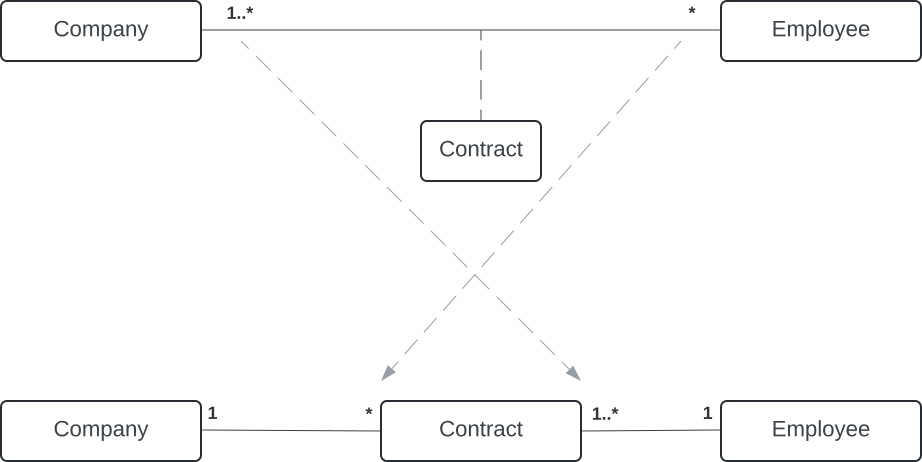
\includegraphics[scale=0.4]{part three/Klassendiagramme - Erweiterte Konzepte und Paketdiagramme/img/assoziationsklasse}
    \caption{Darstellung einer Assoziation mit Hilfe einer Assoziationsklasse (oben) sowie Transformation in gewöhnliche Assoziationen (unten). (Quelle: in Anlehnung an \cite[279, Abb. 4.4-11]{Oes05})}
    \label{fig:assoziationsklasse-cc}
\end{figure}

\clearpage


\section{Sequenzdiagramme}

\begin{tcolorbox}[title=Sequenzdiagramme]
    \textbf{Sequenzdiagramme} stellen Verhalten auf der Ebene einer Interaktion dar.\\
    In der Phase des Klassendesigns werden die Teilnehmer der Interaktionen bestimmt, weshalb Sequenzdiagramme oft in dieser Phase genutzt werden.\\
    In der \textbf{Analysephase} können Sequenzdiagramme eingesetzt werden, um die Kommunikation der bis dahin ausgemachten \textbf{Geschäftsobjekte} zu modellieren, oder um \textbf{Anwendungsfälle} weiter zu spezifizieren.
\end{tcolorbox}
\clearpage

\section{Aggregation}

\begin{tcolorbox}[title=Aggregation]
    Eine \textbf{Aggregation} ist in ihrer \semantischen Aussage unscharf (vgl.~\cite[40]{Buh09}).\\
    Sie beschreibt eine \textit{Ganzes}-\textit{Teile}-Beziehung, aber die \textit{Teile} können zu mehreren verschiedenen \textit{Ganzen} gehören.\\
    Außerdem kann ein Teil dem \textit{Ganzen} jederzeit wieder entnommen werden und das \textit{Ganze} ist nicht verantwortlich für das Erstellen der \textit{Teile}, weshalb Implementierungen beim Hinzufügen von Teilen oft schon fertige Objekte erwarten, die jeweils eines der \textit{Teile} repräsentieren.\\
    Aggregationsbeziehungen werden durch eine nicht-gefüllte Raute an der Seite der Klasse, die das Ganze repräsentiert, dargestellt.
\end{tcolorbox}
\clearpage

\section{Komposition}

\begin{tcolorbox}[title=Komposition]
    Bei einer \textbf{Komposition} handelt es sich um eine \textit{Ganzes}-\textit{Teile}-Beziehung, bei der das \textit{Ganze} verantwortlich für die Erstellung und Beseitigung der \textit{Teile} ist.
    Außerdem sind die \textit{Teile} an die \textbf{Existenz} des \textit{Ganzen} gebunden.\\
    \textit{Teile} gehören immer zu \textit{genau einem} \textit{Ganzen}.\\
    Eine Komposition wird dargestellt durch eine gefüllte Raute an der Klassenbox, die das \textit{Ganze} repräsentiert.
\end{tcolorbox}
\clearpage

\section{Paketdiagramm}

\begin{tcolorbox}[title=Komposition]
    \textbf{Paketdiagramme} zeigen Pakete und ihre Abhängigkeiten und werden in frühen Designphasen genutzt, um Strukturen (großer Systeme) aufzuzeigen.\\

    \noindent
    Elemente sollten so in Paketen gruppiert werden, dass ihr \textbf{funktionaler Zusammenhalt} (\textit{Kohäsion}, s. Abschnitt~\ref{subsec:hohe-kohasion}) klar wird.\\
    Hierdurch kann vermieden werden, dass Änderungen einer Klasse eines Paketes auch Änderungen außerhalb des Paketes erfordern.\\
    Außerdem erhöht sich die Wahrscheinlichkeit, dass einzelne Pakete als solche in anderen Projekten wiederverwendet werden können.\\

    \noindent
    In Paketdiagrammen können Beziehungen über folgende Schlüsselwörter deutlich gemacht werden:

    \begin{itemize}
        \item \guillemotleft import\guillemotright
        \item[] $\rightarrow$ \textbf{public-Import} zwischen Quell- und Zielpaket; Quellpaket kann die öffentlichen Elemente des Zielpaketes unter Verwendung des unqualifizierten und des qualifizierten Namens verwenden; die importierten Elemente sind auch für Pakete sichtbar, die das Quellpaket importieren
        \item \guillemotleft access\guillemotright
        \item[] $\rightarrow$ \textbf{privater Import} zwischen Quell- und Zielpaket; Zugriff auf Elemente des importierten Paketes ohne qualifizierenden Namen möglich; der Import eines Paketes in \textbf{Java} entspricht der \guillemotleft access\guillemotright-Beziehung
        \item \guillemotleft merge\guillemotright
        \item[] $\rightarrow$ Bei einem \textbf{merge} werden Elemente eines Zielpaketes in das Quellpaket
   \end{itemize}
\end{tcolorbox}
\clearpage

\section{Anwendungsfalldiagramm}

\begin{tcolorbox}[title=Anwendungsfalldiagramm]
    Die \textbf{Anwendungsfallanalyse} wird im Rahmen der \textbf{Anforderungsspezifikation} eingesetzt.\\

    \noindent
    Anwendungsfalldiagramme sind das am häufigsten eingesetzte Mittel zur Aufnahme und Darstellung von \textbf{Anforderungen}.\\
    Sie beschreiben selbst kein Verhalten und keine Abläufe, sondern zeigen nur die Zusammenhänge der an Anwendungsfällen beteiligten Modellelemente und sind somit ein Hilfsmittel zur Anforderungsermittlung und Verwaltung.\\

    \noindent
    Zu den wichtigsten Schritten einer Anwendungsfallanalyse gehören:
    \begin{enumerate}
        \item Akteure identifizieren
        \item Anwendungsfälle identifizieren
        \item Beschreiben der Akteure und Anwendungsfälle
        \item Identifizieren von \textit{Schlüsselobjekten}, die das System verwaltet
        \item Identifizieren der wichtigsten Anwendungsfälle (Priorisierung)
        \item detailliertere Beschreibung der Anwendungsfälle
        \item Strukturierung des Anwendungsfalldiagramms
    \end{enumerate}

    \noindent
    Anwendungsfälle beschreiben das \textbf{Szenario} der Nutzung, und nicht Features des Systems.
\end{tcolorbox}

\clearpage

\input{chapters/Anhang/CheatSheets/SE3/Aktivitätsdiagramm}
\clearpage

\section{Zustandsautomat}

\begin{tcolorbox}[title=Zustandsautomat]
    Mit \textbf{Zustandsautomaten} kann das \textit{Verhalten} von Systemen modelliert werden, wobei die \textit{Reaktionen} des Systems im Mittelpunkt stehen, und nicht die \textit{Aktionen}, wie bspw. bei den \textbf{Aktivitätsdiagrammen}.\\

    \noindent
        Ein \textbf{Zustandsautomat} kann den \textit{Lebensweg} eines Objektes modellieren, weshalb Zustandsautomaten oft im \textbf{Entwurf} als Ergänzung zu den \textbf{Klassendiagrammen} eingesetzt werden.
\end{tcolorbox}

\begin{figure}
    \centering
    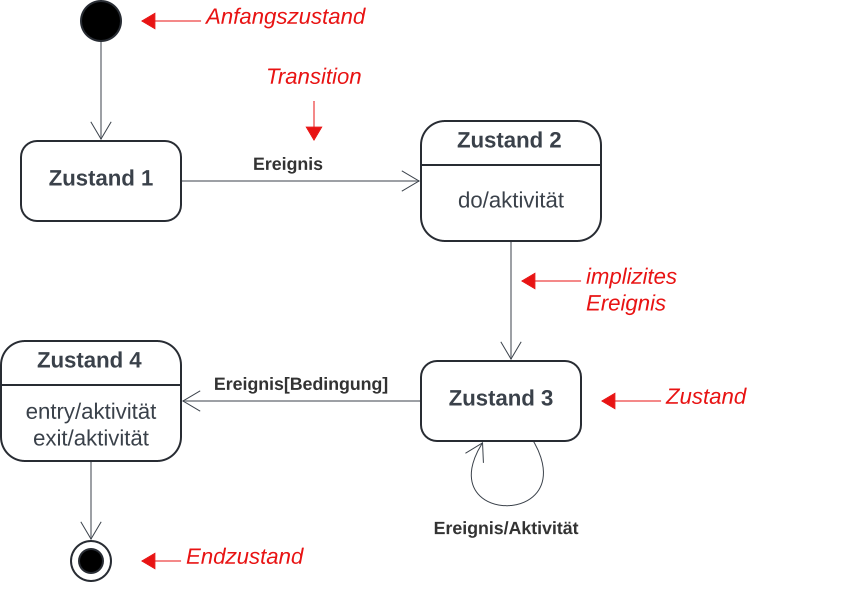
\includegraphics[scale=0.4]{part three/Zustandsautomaten/img/statechartdiagramnotation}
    \caption{Elemente eines einfachen Zustandsautomaten. Eine Transitionen wird durch ein \textbf{Ereignis} ausgelöst, das ein \textit{Signal}, ein \textit{Operationsaufruf} oder auch eine bestimmte \textit{Attributänderung} sein kann. (Quelle: in Anlehnung an \cite[90, Abb. 2.11-6]{Bal05})}
    \label{fig:statechartdiagramnotation-cc}
\end{figure}

\begin{minted}[fontsize=\small]{java}
// Beispiel für eine Implementierung eines
// Parkscheinautomaten als Zustandsautomat in Java
class Parkscheinautomat {

  // zustände
  private final int BEREIT = 0;
  private final int ZAHLUNG = 1;
  private final int ABBRUCH = 2;
  private final int BELEG   = 3;

  // Zustand; wird initial beim Starten
  // des Automaten gesetzt
  private int zustand;

  // Methoden lösen Aktionen beim Eintritt
  // in die jeweiligen Zustände aus
  private int zahlung() {
    // verarbeiten
    // danach neuen Zustand zurückliefern...
    ...
    return BEREIT;
  }

   ...

  private void bereit() {
    while (true) {
      // eingabe überprüfen und
      // ggf. Zustandswechsel auslösen:
      // Zustand als Attribut setzen
      ...
    }
  }

  public void start() {
    zustand = BEREIT;

    while(true) {
      switch (zustand) {
        case BEREIT:
          zustand = bereit();
        // ... weiteres Verhalten
        ...
      }
    }
  }
}
\end{minted}
\clearpage
	

\section{Inhalt SE3}

\section*{1. Übersicht UML}

\subsection*{Lernziele}
\begin{itemize}
    \item einen Einblick in den Sprachaufbau der UML 2.0 gewinnen
    \item einen Überblick über die Diagramme der UML 2.0 und deren Zweck haben
\end{itemize}

\subsection*{Zusammenfassung}
\begin{itemize}
    \item Die \textbf{UML} ist eine weit verbreitete Modellierungssprache zur Modellierung objektorientierter Softwaresysteme.
    \item Die UML 2.0 Spezifikation besteht aus vier Teilen:
    \begin{enumerate}
        \item \textbf{Superstructure}: Diagrammtypen
        \item \textbf{Infrastructure}: Modellierungskonzepte
        \item \textbf{OCL}: formale Sprache zur Formulierung von Einschränkungen
        \item \textbf{Diagram Interchange}: Austauschformate
    \end{enumerate}
    \item Die UML kann im \textbf{Sketching} oder \textbf{Blueprint Modus} eingesetzt werden, oder als Grundlage für \textbf{automatische Codegenerierung}
    \item Die UML ist an keinen speziellen Entwicklungsprozess gebunden
\end{itemize}

\section*{2. Klassendiagramme}

\subsection*{Lernziele}
\begin{itemize}
    \item wissen, wie Klassendiagramme im Entwicklungsprozess eingesetzt werden
    \item Klassendiagramme für Analyse- und Designentscheidungen einsetzen können
    \item die wichtigsten Modellierungskonzepte kennen
    \item sinnvolle Klassendiagramme erstellen und Java-Implementierungen ableiten können
    \item Klassendiagramme aus Java Quellcode erzeugen können
\end{itemize}

\subsection*{Zusammenfassung}

\begin{itemize}
    \item \textbf{Klassendiagramme} dienen zur \textbf{strukturellen Darstellung} von Softwaresystemen
    \item hierbei werden Klassen und \textbf{Beziehungen} zwischen Klassen dargestellt
    \item Properties können durch die \textbf{Attribut}- oder \textbf{Assoziationsnotation} modelliert werden
    \item Operationen werden als separate Zeile in ihrem Compartment dargestellt
    \item im Klassendiagramm können auch \textbf{Generalisierungsbeziehungen} modelliert werden
    \item \textbf{Abhängigkeitsbeziehungen} drücken ein Verhältnis zwischen \textbf{Client} und \textbf{Supplier} aus
\end{itemize}

\section*{3. Objektorientierter Entwurf}

\subsection*{Lernziele}
\begin{itemize}
    \item das Wesen einer Interaktion kennen
    \item wissen, wie Sequenzdiagramme im Entwicklungsprozess eingesetzt werden
    \item Sequenzdiagramme für Analyse- und Designentscheidungen sowie zur Darstellung von Kontrollflüssen einsetzen können
    \item die wichtigsten Modellierungskonzepte kennen
    \item sinnvolle Sequenzdiagramme erstellen und Java-Implementierungen ableiten können
    \item Sequenzdiagramme aus Java Quellcode erzeugen können
\end{itemize}

\subsection*{Zusammenfassung}

\begin{itemize}
    \item Sequenzdiagramme sind \textbf{Verhaltensdiagramme}
    und können im gesamten Entwicklungszyklus zur Modellierung von Interaktionen angewendet werden
    \item Interaktionen bestehen im Wesentlichen aus dem Nachrichtenaustausch zwischen verschiedenen Kommunikationspartnern
    \item in den meisten Fällen wird die Kommunikation von Objekten von Klassen modelliert, aber es können auch Teilnehmer auf anderen Ebenen modelliert werden
    \item gewöhnlich gibt ein Sequenzdiagramm einen \textbf{Anwendungsfall} (\textit{Szenario}) wieder
    \item sie dienen nicht dazu, um Zustandsänderungen darzustellen (hierfür werden Zustandsdiagramme verwendet)
    \item Sequenzdiagramme sind \textit{nicht} gut geeignet für die Darstellung von
    \begin{itemize}
        \item nebenläufigem Verhalten (\textit{asynchrone} Nachrichten, \textit{kombiniertes Fragment})
        \item Schleifen und alternativem Verhalten (\textit{kombinierte Fragmente})
        \item[] $\rightarrow$  für beide Fälle sind \textbf{Aktivitätsdiagramme} besser geeignet
    \end{itemize}
\end{itemize}

\section*{4. Klassendiagramme - Erweiterte Konzepte und Paketdiagramme}

\subsection*{Lernziele}
\begin{itemize}
    \item erweiterte Modellierungskonzepte in Klassendiagrammen für den Detailentwurf von Systemen kennen
    \item die Konsequenzen dieser Konzepte in der Implementierung kennen
    \item wissen, wie Paketdiagramme im Entwicklungsprozess eingesetzt werden
    \item die Modellierungskonzepte in Paketdiagrammen kennen
    \item anhand von Paketdiagrammen Software-Architekturen gestalten und bewerten können
\end{itemize}

\subsection*{Zusammenfassung}

\begin{itemize}
    \item Die vorgestellten erweiterten Konzepte werden vor allem im \textbf{Feinentwurf} von Klassenstrukturen eingesetzt.
    \item Generell gilt, dass die Spezifikationen von Objekten und Properties nur so detailliert ausgeführt werden sollen, wie nötig: Sind Details für das Verständnis unnötig, sollte darauf verzichtet werden.
    \item \textbf{Generalisierungsbeziehungen} sollten grundsätzlich modelliert werden.
    \item Ist eine \textbf{Komposition} statt einer Generalisierung für den Sachverhalt möglich, sollte diese verwendet werden: ``Favor object composition over inheritance.`` (\cite[19 f.]{GHJV94})
    \item \textbf{Kompositionsbeziehungen} geben eindeutige Impulse für eine Implementierung, \textbf{Aggregationsbeziehungen} sind in ihrer semantischen Aussage nicht sehr eindeutig
    \item \textbf{Assoziationsklassen} sind in ihrer frühen Designphase empfehlenswert, die Realisierung (mit {bspw.} Java) erfordert aber eine Transformation in eine volle Klasse, wobei die Multiplizitäten angepasst werden müssen
    \item Elemente können in \textbf{Paketen} zusamengefasst und unter einem gemeinsamen Namensraum gruppiert werden
\end{itemize}

\section*{4. Anwendungsfalldiagramm (Use-Case-Diagramm)}

\subsection*{Lernziele}
\begin{itemize}
    \item wissen, wie die Anwendungsfallanalyse im Rahmen der Anforderungsspezifikation eingesetzt wird
    \item Prozessschritte der Anwendungsfallanalyse beherrschen
    \item die wichtigsten Modellierungskonzepte in Anwendungsfalldiagrammen kennen
    \item den Aufbau einer Anwendungsfallbeschreibung kennen
\end{itemize}

\subsection*{Zusammenfassung}

\begin{itemize}
    \item \textbf{Anwendungsfalldiagramme} besitzen eine einfache Notation, um \textbf{Akteure} und \textbf{Anwendungsfälle} eines \textbf{Systems} grafisch darzustellen
    \item auf Basis eines Anwendungsfalldiagramms lässt sich ermitteln, ob die Anwendungsfälle gewünschtes Verhalten realisieren bzw. Beziehungen zu einem oder mehreren Akteuren haben
    \item Anwendungsfälle und Akteure \textit{müssen} zusätzlich textlich beschrieben werden
\end{itemize}

\section*{5. Aktivitätsdiagramme}

\subsection*{Lernziele}
\begin{itemize}
    \item wissen, wie Aktivitätsdiagramme im Rahmen der Verhaltensanalyse in verschiedenen Prozessphasen eingesetzt werden können
    \item die wichtigsten Modellierungskonzepte in Aktivitätsdiagrammen kennen
    \item Aktivitätsdiagramme interpretieren, erstellen und implementieren können
\end{itemize}

\subsection*{Zusammenfassung}

\begin{itemize}
    \item \textbf{Aktivitätsdiagramme} gehören zu den \textbf{Verhaltensdiagrammen} und können im \textit{gesamten} \textbf{Entwicklungsprozess} eingesetzt werden
    \item durch ein Aktivitätsdiagramm kann gezeigt werden, wie \textbf{Verhalten} realisiert wird
    \item es können mehrere \textbf{Aktivitäten} dargestellt werden
    \item \textbf{Aktivitätskanten} und \textbf{Aktivitätsknoten} werden zur Beschreibung von Verhalten verwendet
\end{itemize}

\section*{5. Zustandsautomaten}

\subsection*{Lernziele}
\begin{itemize}
    \item wissen, wie Zustandsdiagramme im Rahmen der Verhaltensanalyse einzelner Objekte eingesetzt werden können
    \item die wichtigsten Modellierungskonzepte in Zustandsdiagrammen kennen
    \item Zustandsdiagramme interpretieren, erstellen und implementieren können
\end{itemize}

\subsection*{Zusammenfassung}

\begin{itemize}
    \item Das \textbf{Zustandsdiagramm} gehört wie das \textbf{Aktivitätsdiagramm} zu den \textbf{Verhaltensdiagrammen}.
    \item Ein Zustandsdiagramm zeigt den \textbf{Lebensweg} eines \textbf{Objektes}.
    \item \textbf{Attributwerte} bestimmen den Zustand eines Objektes.
    \item \textbf{Transitionen} zwischen Zuständen werden durch \textbf{Guards} und \textbf{Events} gesteuert.
    \item Während der Transitionen können \textbf{Effekte} (\textit{Aktivitäten}) realisiert werden.
    \item Die Modellierung \textbf{zusammengesetzter Zustände} ist ebenfalls möglich.
    \item Für die Darstellung \textbf{paralleler} oder  \textbf{konkurrierender} Abläufe können \textbf{Regionen} modelliert werden.
\end{itemize}
\clearpage


\section{UML Modellierung}

\begin{tcolorbox}[title=UML Modellierung]
    \textbf{Modelle} haben die Aufgabe, den Bezug zum Original (Programm, Softwaresystem) herzustellen, sowie zu der \textit{Anwendungsumgebung}.\\
    Ein \textbf{Modell} enthält alle \textbf{Modellelemente}, die zur Beschreibung eines Softwaresystems nötig sind.\\

    \noindent
    Ein \textbf{Modellelement} wird als Element in einem UML Modell von einem Benutzer erstellt und auf verschiedenen \textbf{Diagrammen} (Struktur-/Verhaltensdiagrammen) platziert, und wird durch die \textbf{UML Modellierungskonzepte} als Metaklasse des \textbf{Metamodells} der UML beschrieben: \textbf{Modellelemente} werden aus Modellierungskonzepten instanziiert.\\

    \noindent
       Das \textbf{UML Metamodell} regelt, in welchem Zusammenhang \textbf{UML Modellierungskonzepte} in Modellen auftreten dürfen, und welche Eigenschaften und Beziehungen zu anderen Sprachelementen zulässig sind.\\

       \noindent
       Die im \textbf{Metamodell} verwendeten Erklärungen basieren auf einer abstrakten Syntax, für deren Beschreibung eine Untermenge (\textit{Klassendiagramme}) der UML verwendet wird.\\
        Die \textbf{Semantik} der Modellierungskonzepte wird textlich beschrieben, zur Formalisierung von Regeln für die syntaktische Korrektheit wird die \textbf{OCL} (\textit{Object Constraint Language}) verwendet.
\end{tcolorbox}

\begin{figure}
    \centering
    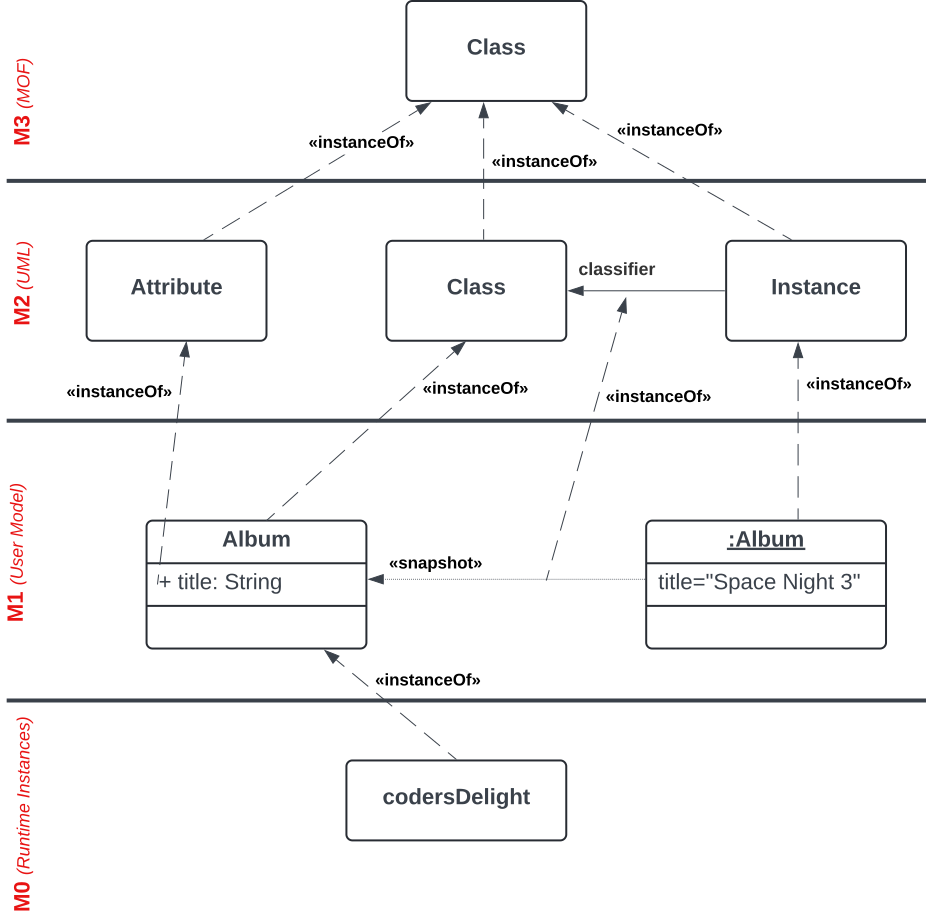
\includegraphics[scale=0.4]{part three/Einführung/img/metamodel}
    \caption{Beispiel für die verschiedenen Schichten der Metamodell Hierarchie.
        In der original Abbildung sind die Pfeilspitzen offen. (Quelle: in Anlehnung an S. 20, Figure 7.8, \url{https://www.omg.org/spec/UML/2.4.1/Infrastructure/PDF}, abgerufen 01.05.2024}
    \label{fig:metamodel-cc}
\end{figure}

\clearpage


\section{Strukturdiagramme}

\begin{tcolorbox}[title=Strukturdiagramme]
    In den \textbf{Strukturdiagrammen} werden \textbf{statische Strukturaspekte} eines Systems betrachtet.
    Für eine Systemmodellierung können alle dieser 6 Diagramme verwendet werden.

    \begin{itemize}
        \item \textbf{Klassendiagramm}: Das \textbf{Klassendiagramm} wird verwendet, um ein objektorientiertes System zu beschreiben.
        \item \textbf{Paketdiagramm}: Ein \textbf{Paketdiagramm} zeigt die Pakete eines Systems und deren Beziehungen.
        \item \textbf{Komponentendiagramm}: Stellt Komponenten oder auch \textit{Subsysteme} mit definierten Interfaces dar, um bspw. \textbf{Architekturdesign} darzustellen.
        \item \textbf{Verteilungsdiagramm}: Beschreibt eine Menge von Knoten, die die \textit{Ausführungsarchitektur} eines Systems definieren können, wobei Knoten i.d.R. \textit{Geräte} oder \textit{Softwareablaufumgebungen repräsentieren}.
        \item \textbf{Kompositionsstrukturdiagramm}: Stellt die \textbf{Komposition} von \textit{Systemstrukturen} (Klassen, Komponenten, Gesamtsystem) in einem bestimmten \textit{Kontext} mit einem bestimmten \textit{Ziel} dar (vgl. \cite[9]{Buh09}).
        \item \textbf{Objektdiagramm}: Momentaufnahme eines Systems zu genau einem \textit{Zeitpukt} während der Ausführung
    \end{itemize}

\end{tcolorbox}
\clearpage

\section{Verhaltensdiagramme}

\begin{tcolorbox}[title=Verhaltensdiagramme]
    \textbf{Verhaltensdiagramme} stellen \textit{Dynamik}, \textit{interne Abläufe} und das \textit{Zusammenspiel} der Systemteile dar, um eine Spezifikation zu vervollständigen.

    \begin{itemize}
        \item \textbf{Anwendungsfalldiagramm}: Dienen zur \textit{Spezifizierung} und \textit{Formalisierung} von \textit{Systemanforderungen}, unter Berücksichtigung von \textbf{Akteuren}, \textbf{Systemen} und \textbf{Anwendungsfällen}
        \item \textbf{Zustandsdiagramm}: Auch \textbf{Zustandsautomaten}; zeigen für ein einzelnes Objekt Zustandsänderungen während der Lebenszeit
        \item \textbf{Aktivitätsdiagramme}: Werden zur Modellierung von \textit{Kontroll}- oder \textit{Objektflüssen} oder zur Darstellung von \textit{Programmlogik} genutzt.
        \item \textbf{Interaktionsdiagramme}: Stellen das Zusammenspiel mehrerer Kommunikationspartner dar.
        Es gibt unterschiedliche Typen von Interaktionsdiagrammen, die Interaktionen auf verschiedenen \textit{Abstraktionsebenen} modellieren:
        \begin{itemize}
            \item \textbf{Sequenzdiagramm}: Zeigt den Verlauf einer Interaktion in zwei Dimensionen, \textit{Kommunikationspartner} und die Nachrichten in ihrer \textit{zeitlichen Abfolge}
            \item \textbf{Kommunikationsdiagramm}: hebt die Kommunikationsbeziehungen zwischen den Partnern hervor
            \item \textbf{Timing Diagramm}: hebt die zeitlichen Aspekte einer Interaktion hervor
            \item \textbf{Interaktionsüberblickdiagramm}: Spezialfall des \textbf{Aktivitätsdiagramms} - statt Aktionen und Aktivitäten können das \textbf{Sequenz}-, \textbf{Kommunikations}- und das \textbf{Timing}-Diagramm als Knoten verwendet werden.
        \end{itemize}
        Alle verwenden dieselben Grundelemente: \textit{Lebenslinien} der Akteure und Nachrichten, die zwischen diesen ausgetauscht werden.
    \end{itemize}
\end{tcolorbox}

\clearpage


\section{Klassendiagramm}

\begin{tcolorbox}[title=Klassendiagramm]
    Das \textbf{Klassendiagramm} beschreibt die Klassen eines Systems und die statischen Beziehungen zwischen ihnen.\\
    Sie werden in Form von Domainklassen bei der \textbf{Analyse} und als detaillierte Entwürfe von Systemklassen als \textit{Blueprint} im \textbf{gesamten Entwicklungsprozess} eingesetzt.

\end{tcolorbox}
\clearpage


\section{Assoziationsklasse (Attributierte Assoziation)}

\begin{tcolorbox}[title=Assoziationsklasse (Attributierte Assoziation)]
Eine \textbf{Assoziationsklasse} erlaubt das Hinzufügen von Operationen und Attributen zu einer Assoziation (\cite[43]{Buh09}).\\
Assoziationsklassen werden in der \textbf{Analyse} in Modellen verwendet und in dem \textbf{Entwurf} in eigenständige Klassen transformiert.\\

\noindent
Assoziationsklassen werden in der \textbf{Analyse} in Modellen verwendet und in dem \textbf{Entwurf} in eigenständige Klassen transformiert.

\blockquote[{\cite[277]{Oes05}}]{
    Eine attributierte Assoziation ist immer dann nahe liegend, wenn Attribute oder Operationen gefunden werden, die weder der einen noch der anderen Klasse zugeordnet werden können, weil sie nämlich Eigenschaften der Beziehung selbst sind.
}.\\

Bei einer attributierten Assoziation dürfen zwei beteiligte Objekte maximal nur eine Beziehung zueinander haben (vgl.~\cite[277]{Oes05})\footnote{
    \textit{Ostereich} führt dies ebenda auf Seite 278 weiter aus, in dem er beschreibt, wie eine attributierte Assoziation für ein \textit{Beschäftigtenverhältnis} zwischen \textit{Mitarbeiter} und \textit{Unternehmen} modelliert wird. Dabei wird davon ausgegangen, dass ein \textit{Mitarbeiter} nur über \textit{ein} Arbeitsverhältnis mit einem \textit{Unternehmen} in Beziehung stehen kann. Bestehen mehrere Arbeitsverhältnisse (\textit{Mitarbeiter} hat zu unterschiedlichen Zeitpunkten für das \textit{Unternehmen} gearbeitet), kann die attributierte Assoziation nicht verwendet werden.\\

\noindent
Wird eine attributierte Assoziation in eine gewöhnliche Assoziation transformiert, muss darauf geachtet werden, die Multiplizitäten richtig zu setzen (s. Abbildung~\ref{fig:assoziationsklasse}).
\end{tcolorbox}

\begin{figure}
    \centering
    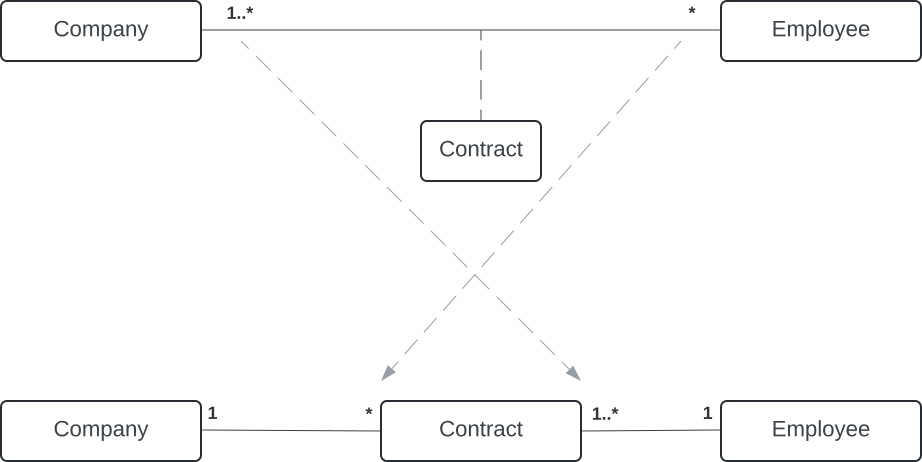
\includegraphics[scale=0.4]{part three/Klassendiagramme - Erweiterte Konzepte und Paketdiagramme/img/assoziationsklasse}
    \caption{Darstellung einer Assoziation mit Hilfe einer Assoziationsklasse (oben) sowie Transformation in gewöhnliche Assoziationen (unten). (Quelle: in Anlehnung an \cite[279, Abb. 4.4-11]{Oes05})}
    \label{fig:assoziationsklasse-cc}
\end{figure}

\clearpage


\section{Sequenzdiagramme}

\begin{tcolorbox}[title=Sequenzdiagramme]
    \textbf{Sequenzdiagramme} stellen Verhalten auf der Ebene einer Interaktion dar.\\
    In der Phase des Klassendesigns werden die Teilnehmer der Interaktionen bestimmt, weshalb Sequenzdiagramme oft in dieser Phase genutzt werden.\\
    In der \textbf{Analysephase} können Sequenzdiagramme eingesetzt werden, um die Kommunikation der bis dahin ausgemachten \textbf{Geschäftsobjekte} zu modellieren, oder um \textbf{Anwendungsfälle} weiter zu spezifizieren.
\end{tcolorbox}
\clearpage

\section{Aggregation}

\begin{tcolorbox}[title=Aggregation]
    Eine \textbf{Aggregation} ist in ihrer \semantischen Aussage unscharf (vgl.~\cite[40]{Buh09}).\\
    Sie beschreibt eine \textit{Ganzes}-\textit{Teile}-Beziehung, aber die \textit{Teile} können zu mehreren verschiedenen \textit{Ganzen} gehören.\\
    Außerdem kann ein Teil dem \textit{Ganzen} jederzeit wieder entnommen werden und das \textit{Ganze} ist nicht verantwortlich für das Erstellen der \textit{Teile}, weshalb Implementierungen beim Hinzufügen von Teilen oft schon fertige Objekte erwarten, die jeweils eines der \textit{Teile} repräsentieren.\\
    Aggregationsbeziehungen werden durch eine nicht-gefüllte Raute an der Seite der Klasse, die das Ganze repräsentiert, dargestellt.
\end{tcolorbox}
\clearpage

\section{Komposition}

\begin{tcolorbox}[title=Komposition]
    Bei einer \textbf{Komposition} handelt es sich um eine \textit{Ganzes}-\textit{Teile}-Beziehung, bei der das \textit{Ganze} verantwortlich für die Erstellung und Beseitigung der \textit{Teile} ist.
    Außerdem sind die \textit{Teile} an die \textbf{Existenz} des \textit{Ganzen} gebunden.\\
    \textit{Teile} gehören immer zu \textit{genau einem} \textit{Ganzen}.\\
    Eine Komposition wird dargestellt durch eine gefüllte Raute an der Klassenbox, die das \textit{Ganze} repräsentiert.
\end{tcolorbox}
\clearpage

\section{Paketdiagramm}

\begin{tcolorbox}[title=Komposition]
    \textbf{Paketdiagramme} zeigen Pakete und ihre Abhängigkeiten und werden in frühen Designphasen genutzt, um Strukturen (großer Systeme) aufzuzeigen.\\

    \noindent
    Elemente sollten so in Paketen gruppiert werden, dass ihr \textbf{funktionaler Zusammenhalt} (\textit{Kohäsion}, s. Abschnitt~\ref{subsec:hohe-kohasion}) klar wird.\\
    Hierdurch kann vermieden werden, dass Änderungen einer Klasse eines Paketes auch Änderungen außerhalb des Paketes erfordern.\\
    Außerdem erhöht sich die Wahrscheinlichkeit, dass einzelne Pakete als solche in anderen Projekten wiederverwendet werden können.\\

    \noindent
    In Paketdiagrammen können Beziehungen über folgende Schlüsselwörter deutlich gemacht werden:

    \begin{itemize}
        \item \guillemotleft import\guillemotright
        \item[] $\rightarrow$ \textbf{public-Import} zwischen Quell- und Zielpaket; Quellpaket kann die öffentlichen Elemente des Zielpaketes unter Verwendung des unqualifizierten und des qualifizierten Namens verwenden; die importierten Elemente sind auch für Pakete sichtbar, die das Quellpaket importieren
        \item \guillemotleft access\guillemotright
        \item[] $\rightarrow$ \textbf{privater Import} zwischen Quell- und Zielpaket; Zugriff auf Elemente des importierten Paketes ohne qualifizierenden Namen möglich; der Import eines Paketes in \textbf{Java} entspricht der \guillemotleft access\guillemotright-Beziehung
        \item \guillemotleft merge\guillemotright
        \item[] $\rightarrow$ Bei einem \textbf{merge} werden Elemente eines Zielpaketes in das Quellpaket
   \end{itemize}
\end{tcolorbox}
\clearpage

\section{Anwendungsfalldiagramm}

\begin{tcolorbox}[title=Anwendungsfalldiagramm]
    Die \textbf{Anwendungsfallanalyse} wird im Rahmen der \textbf{Anforderungsspezifikation} eingesetzt.\\

    \noindent
    Anwendungsfalldiagramme sind das am häufigsten eingesetzte Mittel zur Aufnahme und Darstellung von \textbf{Anforderungen}.\\
    Sie beschreiben selbst kein Verhalten und keine Abläufe, sondern zeigen nur die Zusammenhänge der an Anwendungsfällen beteiligten Modellelemente und sind somit ein Hilfsmittel zur Anforderungsermittlung und Verwaltung.\\

    \noindent
    Zu den wichtigsten Schritten einer Anwendungsfallanalyse gehören:
    \begin{enumerate}
        \item Akteure identifizieren
        \item Anwendungsfälle identifizieren
        \item Beschreiben der Akteure und Anwendungsfälle
        \item Identifizieren von \textit{Schlüsselobjekten}, die das System verwaltet
        \item Identifizieren der wichtigsten Anwendungsfälle (Priorisierung)
        \item detailliertere Beschreibung der Anwendungsfälle
        \item Strukturierung des Anwendungsfalldiagramms
    \end{enumerate}

    \noindent
    Anwendungsfälle beschreiben das \textbf{Szenario} der Nutzung, und nicht Features des Systems.
\end{tcolorbox}

\clearpage

\input{chapters/Anhang/CheatSheets/SE3/Aktivitätsdiagramm}
\clearpage

\section{Zustandsautomat}

\begin{tcolorbox}[title=Zustandsautomat]
    Mit \textbf{Zustandsautomaten} kann das \textit{Verhalten} von Systemen modelliert werden, wobei die \textit{Reaktionen} des Systems im Mittelpunkt stehen, und nicht die \textit{Aktionen}, wie bspw. bei den \textbf{Aktivitätsdiagrammen}.\\

    \noindent
        Ein \textbf{Zustandsautomat} kann den \textit{Lebensweg} eines Objektes modellieren, weshalb Zustandsautomaten oft im \textbf{Entwurf} als Ergänzung zu den \textbf{Klassendiagrammen} eingesetzt werden.
\end{tcolorbox}

\begin{figure}
    \centering
    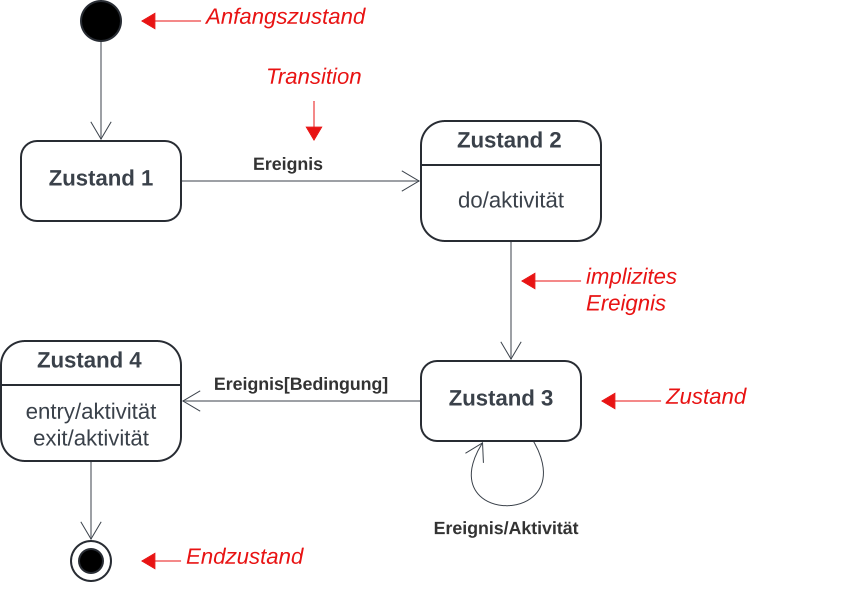
\includegraphics[scale=0.4]{part three/Zustandsautomaten/img/statechartdiagramnotation}
    \caption{Elemente eines einfachen Zustandsautomaten. Eine Transitionen wird durch ein \textbf{Ereignis} ausgelöst, das ein \textit{Signal}, ein \textit{Operationsaufruf} oder auch eine bestimmte \textit{Attributänderung} sein kann. (Quelle: in Anlehnung an \cite[90, Abb. 2.11-6]{Bal05})}
    \label{fig:statechartdiagramnotation-cc}
\end{figure}

\begin{minted}[fontsize=\small]{java}
// Beispiel für eine Implementierung eines
// Parkscheinautomaten als Zustandsautomat in Java
class Parkscheinautomat {

  // zustände
  private final int BEREIT = 0;
  private final int ZAHLUNG = 1;
  private final int ABBRUCH = 2;
  private final int BELEG   = 3;

  // Zustand; wird initial beim Starten
  // des Automaten gesetzt
  private int zustand;

  // Methoden lösen Aktionen beim Eintritt
  // in die jeweiligen Zustände aus
  private int zahlung() {
    // verarbeiten
    // danach neuen Zustand zurückliefern...
    ...
    return BEREIT;
  }

   ...

  private void bereit() {
    while (true) {
      // eingabe überprüfen und
      // ggf. Zustandswechsel auslösen:
      // Zustand als Attribut setzen
      ...
    }
  }

  public void start() {
    zustand = BEREIT;

    while(true) {
      switch (zustand) {
        case BEREIT:
          zustand = bereit();
        // ... weiteres Verhalten
        ...
      }
    }
  }
}
\end{minted}
\clearpage

	\part{Teil 4 - Qualitätssicherung}

\newpage
\section*{Lernziele Teil 4}

\begin{itemize}
    \item Qualität für ein Softwaresystem systematisch definieren können
    \item einen systematischen Überblick über qualitätssichernde Maßnahmen besitzen
    \item angemessene qualitätssichernde Maßnahmen für eine Aufgabe auswählen können
    \item die Qualitätssicherung in kleineren Projekten organisieren können
    \item die wichtigsten qualitätssichernden Maßnahmen wie Reviews und Tests systematisch durchführen können
    \item Werkzeuge zur Qualitätssicherung auswählen und einsetzen können
\end{itemize}

\newpage
	

\section{Inhalt SE3}

\section*{1. Übersicht UML}

\subsection*{Lernziele}
\begin{itemize}
    \item einen Einblick in den Sprachaufbau der UML 2.0 gewinnen
    \item einen Überblick über die Diagramme der UML 2.0 und deren Zweck haben
\end{itemize}

\subsection*{Zusammenfassung}
\begin{itemize}
    \item Die \textbf{UML} ist eine weit verbreitete Modellierungssprache zur Modellierung objektorientierter Softwaresysteme.
    \item Die UML 2.0 Spezifikation besteht aus vier Teilen:
    \begin{enumerate}
        \item \textbf{Superstructure}: Diagrammtypen
        \item \textbf{Infrastructure}: Modellierungskonzepte
        \item \textbf{OCL}: formale Sprache zur Formulierung von Einschränkungen
        \item \textbf{Diagram Interchange}: Austauschformate
    \end{enumerate}
    \item Die UML kann im \textbf{Sketching} oder \textbf{Blueprint Modus} eingesetzt werden, oder als Grundlage für \textbf{automatische Codegenerierung}
    \item Die UML ist an keinen speziellen Entwicklungsprozess gebunden
\end{itemize}

\section*{2. Klassendiagramme}

\subsection*{Lernziele}
\begin{itemize}
    \item wissen, wie Klassendiagramme im Entwicklungsprozess eingesetzt werden
    \item Klassendiagramme für Analyse- und Designentscheidungen einsetzen können
    \item die wichtigsten Modellierungskonzepte kennen
    \item sinnvolle Klassendiagramme erstellen und Java-Implementierungen ableiten können
    \item Klassendiagramme aus Java Quellcode erzeugen können
\end{itemize}

\subsection*{Zusammenfassung}

\begin{itemize}
    \item \textbf{Klassendiagramme} dienen zur \textbf{strukturellen Darstellung} von Softwaresystemen
    \item hierbei werden Klassen und \textbf{Beziehungen} zwischen Klassen dargestellt
    \item Properties können durch die \textbf{Attribut}- oder \textbf{Assoziationsnotation} modelliert werden
    \item Operationen werden als separate Zeile in ihrem Compartment dargestellt
    \item im Klassendiagramm können auch \textbf{Generalisierungsbeziehungen} modelliert werden
    \item \textbf{Abhängigkeitsbeziehungen} drücken ein Verhältnis zwischen \textbf{Client} und \textbf{Supplier} aus
\end{itemize}

\section*{3. Objektorientierter Entwurf}

\subsection*{Lernziele}
\begin{itemize}
    \item das Wesen einer Interaktion kennen
    \item wissen, wie Sequenzdiagramme im Entwicklungsprozess eingesetzt werden
    \item Sequenzdiagramme für Analyse- und Designentscheidungen sowie zur Darstellung von Kontrollflüssen einsetzen können
    \item die wichtigsten Modellierungskonzepte kennen
    \item sinnvolle Sequenzdiagramme erstellen und Java-Implementierungen ableiten können
    \item Sequenzdiagramme aus Java Quellcode erzeugen können
\end{itemize}

\subsection*{Zusammenfassung}

\begin{itemize}
    \item Sequenzdiagramme sind \textbf{Verhaltensdiagramme}
    und können im gesamten Entwicklungszyklus zur Modellierung von Interaktionen angewendet werden
    \item Interaktionen bestehen im Wesentlichen aus dem Nachrichtenaustausch zwischen verschiedenen Kommunikationspartnern
    \item in den meisten Fällen wird die Kommunikation von Objekten von Klassen modelliert, aber es können auch Teilnehmer auf anderen Ebenen modelliert werden
    \item gewöhnlich gibt ein Sequenzdiagramm einen \textbf{Anwendungsfall} (\textit{Szenario}) wieder
    \item sie dienen nicht dazu, um Zustandsänderungen darzustellen (hierfür werden Zustandsdiagramme verwendet)
    \item Sequenzdiagramme sind \textit{nicht} gut geeignet für die Darstellung von
    \begin{itemize}
        \item nebenläufigem Verhalten (\textit{asynchrone} Nachrichten, \textit{kombiniertes Fragment})
        \item Schleifen und alternativem Verhalten (\textit{kombinierte Fragmente})
        \item[] $\rightarrow$  für beide Fälle sind \textbf{Aktivitätsdiagramme} besser geeignet
    \end{itemize}
\end{itemize}

\section*{4. Klassendiagramme - Erweiterte Konzepte und Paketdiagramme}

\subsection*{Lernziele}
\begin{itemize}
    \item erweiterte Modellierungskonzepte in Klassendiagrammen für den Detailentwurf von Systemen kennen
    \item die Konsequenzen dieser Konzepte in der Implementierung kennen
    \item wissen, wie Paketdiagramme im Entwicklungsprozess eingesetzt werden
    \item die Modellierungskonzepte in Paketdiagrammen kennen
    \item anhand von Paketdiagrammen Software-Architekturen gestalten und bewerten können
\end{itemize}

\subsection*{Zusammenfassung}

\begin{itemize}
    \item Die vorgestellten erweiterten Konzepte werden vor allem im \textbf{Feinentwurf} von Klassenstrukturen eingesetzt.
    \item Generell gilt, dass die Spezifikationen von Objekten und Properties nur so detailliert ausgeführt werden sollen, wie nötig: Sind Details für das Verständnis unnötig, sollte darauf verzichtet werden.
    \item \textbf{Generalisierungsbeziehungen} sollten grundsätzlich modelliert werden.
    \item Ist eine \textbf{Komposition} statt einer Generalisierung für den Sachverhalt möglich, sollte diese verwendet werden: ``Favor object composition over inheritance.`` (\cite[19 f.]{GHJV94})
    \item \textbf{Kompositionsbeziehungen} geben eindeutige Impulse für eine Implementierung, \textbf{Aggregationsbeziehungen} sind in ihrer semantischen Aussage nicht sehr eindeutig
    \item \textbf{Assoziationsklassen} sind in ihrer frühen Designphase empfehlenswert, die Realisierung (mit {bspw.} Java) erfordert aber eine Transformation in eine volle Klasse, wobei die Multiplizitäten angepasst werden müssen
    \item Elemente können in \textbf{Paketen} zusamengefasst und unter einem gemeinsamen Namensraum gruppiert werden
\end{itemize}

\section*{4. Anwendungsfalldiagramm (Use-Case-Diagramm)}

\subsection*{Lernziele}
\begin{itemize}
    \item wissen, wie die Anwendungsfallanalyse im Rahmen der Anforderungsspezifikation eingesetzt wird
    \item Prozessschritte der Anwendungsfallanalyse beherrschen
    \item die wichtigsten Modellierungskonzepte in Anwendungsfalldiagrammen kennen
    \item den Aufbau einer Anwendungsfallbeschreibung kennen
\end{itemize}

\subsection*{Zusammenfassung}

\begin{itemize}
    \item \textbf{Anwendungsfalldiagramme} besitzen eine einfache Notation, um \textbf{Akteure} und \textbf{Anwendungsfälle} eines \textbf{Systems} grafisch darzustellen
    \item auf Basis eines Anwendungsfalldiagramms lässt sich ermitteln, ob die Anwendungsfälle gewünschtes Verhalten realisieren bzw. Beziehungen zu einem oder mehreren Akteuren haben
    \item Anwendungsfälle und Akteure \textit{müssen} zusätzlich textlich beschrieben werden
\end{itemize}

\section*{5. Aktivitätsdiagramme}

\subsection*{Lernziele}
\begin{itemize}
    \item wissen, wie Aktivitätsdiagramme im Rahmen der Verhaltensanalyse in verschiedenen Prozessphasen eingesetzt werden können
    \item die wichtigsten Modellierungskonzepte in Aktivitätsdiagrammen kennen
    \item Aktivitätsdiagramme interpretieren, erstellen und implementieren können
\end{itemize}

\subsection*{Zusammenfassung}

\begin{itemize}
    \item \textbf{Aktivitätsdiagramme} gehören zu den \textbf{Verhaltensdiagrammen} und können im \textit{gesamten} \textbf{Entwicklungsprozess} eingesetzt werden
    \item durch ein Aktivitätsdiagramm kann gezeigt werden, wie \textbf{Verhalten} realisiert wird
    \item es können mehrere \textbf{Aktivitäten} dargestellt werden
    \item \textbf{Aktivitätskanten} und \textbf{Aktivitätsknoten} werden zur Beschreibung von Verhalten verwendet
\end{itemize}

\section*{5. Zustandsautomaten}

\subsection*{Lernziele}
\begin{itemize}
    \item wissen, wie Zustandsdiagramme im Rahmen der Verhaltensanalyse einzelner Objekte eingesetzt werden können
    \item die wichtigsten Modellierungskonzepte in Zustandsdiagrammen kennen
    \item Zustandsdiagramme interpretieren, erstellen und implementieren können
\end{itemize}

\subsection*{Zusammenfassung}

\begin{itemize}
    \item Das \textbf{Zustandsdiagramm} gehört wie das \textbf{Aktivitätsdiagramm} zu den \textbf{Verhaltensdiagrammen}.
    \item Ein Zustandsdiagramm zeigt den \textbf{Lebensweg} eines \textbf{Objektes}.
    \item \textbf{Attributwerte} bestimmen den Zustand eines Objektes.
    \item \textbf{Transitionen} zwischen Zuständen werden durch \textbf{Guards} und \textbf{Events} gesteuert.
    \item Während der Transitionen können \textbf{Effekte} (\textit{Aktivitäten}) realisiert werden.
    \item Die Modellierung \textbf{zusammengesetzter Zustände} ist ebenfalls möglich.
    \item Für die Darstellung \textbf{paralleler} oder  \textbf{konkurrierender} Abläufe können \textbf{Regionen} modelliert werden.
\end{itemize}
\clearpage


\section{UML Modellierung}

\begin{tcolorbox}[title=UML Modellierung]
    \textbf{Modelle} haben die Aufgabe, den Bezug zum Original (Programm, Softwaresystem) herzustellen, sowie zu der \textit{Anwendungsumgebung}.\\
    Ein \textbf{Modell} enthält alle \textbf{Modellelemente}, die zur Beschreibung eines Softwaresystems nötig sind.\\

    \noindent
    Ein \textbf{Modellelement} wird als Element in einem UML Modell von einem Benutzer erstellt und auf verschiedenen \textbf{Diagrammen} (Struktur-/Verhaltensdiagrammen) platziert, und wird durch die \textbf{UML Modellierungskonzepte} als Metaklasse des \textbf{Metamodells} der UML beschrieben: \textbf{Modellelemente} werden aus Modellierungskonzepten instanziiert.\\

    \noindent
       Das \textbf{UML Metamodell} regelt, in welchem Zusammenhang \textbf{UML Modellierungskonzepte} in Modellen auftreten dürfen, und welche Eigenschaften und Beziehungen zu anderen Sprachelementen zulässig sind.\\

       \noindent
       Die im \textbf{Metamodell} verwendeten Erklärungen basieren auf einer abstrakten Syntax, für deren Beschreibung eine Untermenge (\textit{Klassendiagramme}) der UML verwendet wird.\\
        Die \textbf{Semantik} der Modellierungskonzepte wird textlich beschrieben, zur Formalisierung von Regeln für die syntaktische Korrektheit wird die \textbf{OCL} (\textit{Object Constraint Language}) verwendet.
\end{tcolorbox}

\begin{figure}
    \centering
    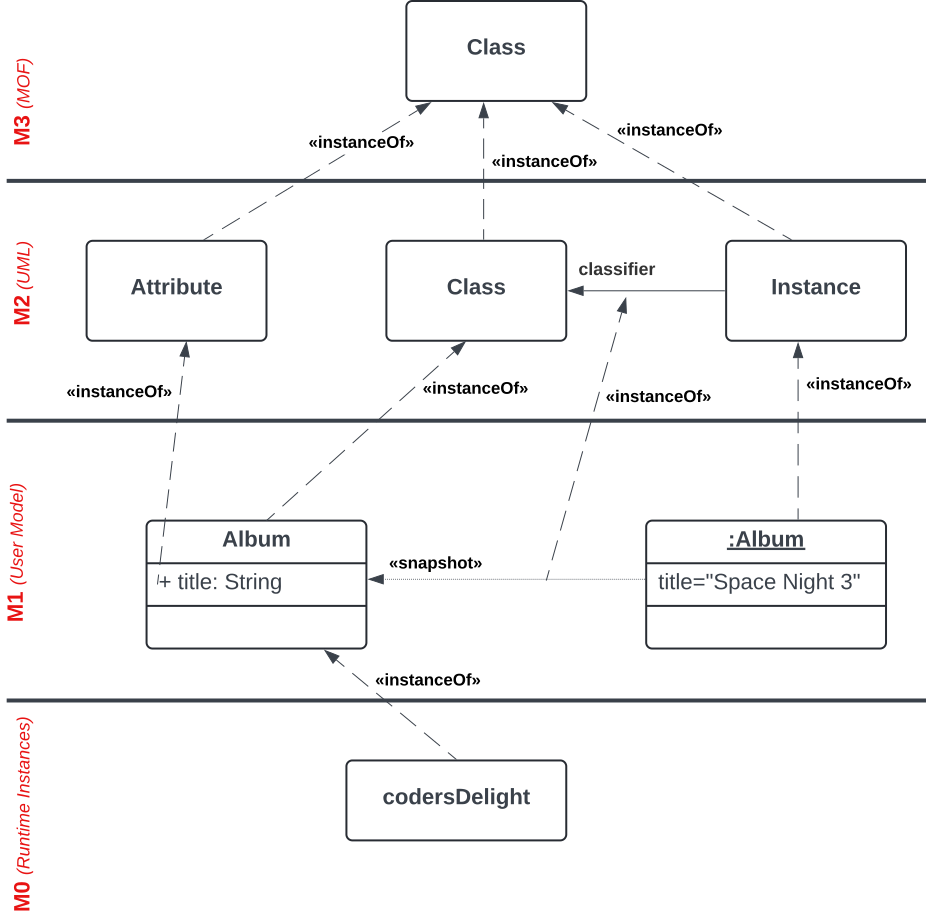
\includegraphics[scale=0.4]{part three/Einführung/img/metamodel}
    \caption{Beispiel für die verschiedenen Schichten der Metamodell Hierarchie.
        In der original Abbildung sind die Pfeilspitzen offen. (Quelle: in Anlehnung an S. 20, Figure 7.8, \url{https://www.omg.org/spec/UML/2.4.1/Infrastructure/PDF}, abgerufen 01.05.2024}
    \label{fig:metamodel-cc}
\end{figure}

\clearpage


\section{Strukturdiagramme}

\begin{tcolorbox}[title=Strukturdiagramme]
    In den \textbf{Strukturdiagrammen} werden \textbf{statische Strukturaspekte} eines Systems betrachtet.
    Für eine Systemmodellierung können alle dieser 6 Diagramme verwendet werden.

    \begin{itemize}
        \item \textbf{Klassendiagramm}: Das \textbf{Klassendiagramm} wird verwendet, um ein objektorientiertes System zu beschreiben.
        \item \textbf{Paketdiagramm}: Ein \textbf{Paketdiagramm} zeigt die Pakete eines Systems und deren Beziehungen.
        \item \textbf{Komponentendiagramm}: Stellt Komponenten oder auch \textit{Subsysteme} mit definierten Interfaces dar, um bspw. \textbf{Architekturdesign} darzustellen.
        \item \textbf{Verteilungsdiagramm}: Beschreibt eine Menge von Knoten, die die \textit{Ausführungsarchitektur} eines Systems definieren können, wobei Knoten i.d.R. \textit{Geräte} oder \textit{Softwareablaufumgebungen repräsentieren}.
        \item \textbf{Kompositionsstrukturdiagramm}: Stellt die \textbf{Komposition} von \textit{Systemstrukturen} (Klassen, Komponenten, Gesamtsystem) in einem bestimmten \textit{Kontext} mit einem bestimmten \textit{Ziel} dar (vgl. \cite[9]{Buh09}).
        \item \textbf{Objektdiagramm}: Momentaufnahme eines Systems zu genau einem \textit{Zeitpukt} während der Ausführung
    \end{itemize}

\end{tcolorbox}
\clearpage

\section{Verhaltensdiagramme}

\begin{tcolorbox}[title=Verhaltensdiagramme]
    \textbf{Verhaltensdiagramme} stellen \textit{Dynamik}, \textit{interne Abläufe} und das \textit{Zusammenspiel} der Systemteile dar, um eine Spezifikation zu vervollständigen.

    \begin{itemize}
        \item \textbf{Anwendungsfalldiagramm}: Dienen zur \textit{Spezifizierung} und \textit{Formalisierung} von \textit{Systemanforderungen}, unter Berücksichtigung von \textbf{Akteuren}, \textbf{Systemen} und \textbf{Anwendungsfällen}
        \item \textbf{Zustandsdiagramm}: Auch \textbf{Zustandsautomaten}; zeigen für ein einzelnes Objekt Zustandsänderungen während der Lebenszeit
        \item \textbf{Aktivitätsdiagramme}: Werden zur Modellierung von \textit{Kontroll}- oder \textit{Objektflüssen} oder zur Darstellung von \textit{Programmlogik} genutzt.
        \item \textbf{Interaktionsdiagramme}: Stellen das Zusammenspiel mehrerer Kommunikationspartner dar.
        Es gibt unterschiedliche Typen von Interaktionsdiagrammen, die Interaktionen auf verschiedenen \textit{Abstraktionsebenen} modellieren:
        \begin{itemize}
            \item \textbf{Sequenzdiagramm}: Zeigt den Verlauf einer Interaktion in zwei Dimensionen, \textit{Kommunikationspartner} und die Nachrichten in ihrer \textit{zeitlichen Abfolge}
            \item \textbf{Kommunikationsdiagramm}: hebt die Kommunikationsbeziehungen zwischen den Partnern hervor
            \item \textbf{Timing Diagramm}: hebt die zeitlichen Aspekte einer Interaktion hervor
            \item \textbf{Interaktionsüberblickdiagramm}: Spezialfall des \textbf{Aktivitätsdiagramms} - statt Aktionen und Aktivitäten können das \textbf{Sequenz}-, \textbf{Kommunikations}- und das \textbf{Timing}-Diagramm als Knoten verwendet werden.
        \end{itemize}
        Alle verwenden dieselben Grundelemente: \textit{Lebenslinien} der Akteure und Nachrichten, die zwischen diesen ausgetauscht werden.
    \end{itemize}
\end{tcolorbox}

\clearpage


\section{Klassendiagramm}

\begin{tcolorbox}[title=Klassendiagramm]
    Das \textbf{Klassendiagramm} beschreibt die Klassen eines Systems und die statischen Beziehungen zwischen ihnen.\\
    Sie werden in Form von Domainklassen bei der \textbf{Analyse} und als detaillierte Entwürfe von Systemklassen als \textit{Blueprint} im \textbf{gesamten Entwicklungsprozess} eingesetzt.

\end{tcolorbox}
\clearpage


\section{Assoziationsklasse (Attributierte Assoziation)}

\begin{tcolorbox}[title=Assoziationsklasse (Attributierte Assoziation)]
Eine \textbf{Assoziationsklasse} erlaubt das Hinzufügen von Operationen und Attributen zu einer Assoziation (\cite[43]{Buh09}).\\
Assoziationsklassen werden in der \textbf{Analyse} in Modellen verwendet und in dem \textbf{Entwurf} in eigenständige Klassen transformiert.\\

\noindent
Assoziationsklassen werden in der \textbf{Analyse} in Modellen verwendet und in dem \textbf{Entwurf} in eigenständige Klassen transformiert.

\blockquote[{\cite[277]{Oes05}}]{
    Eine attributierte Assoziation ist immer dann nahe liegend, wenn Attribute oder Operationen gefunden werden, die weder der einen noch der anderen Klasse zugeordnet werden können, weil sie nämlich Eigenschaften der Beziehung selbst sind.
}.\\

Bei einer attributierten Assoziation dürfen zwei beteiligte Objekte maximal nur eine Beziehung zueinander haben (vgl.~\cite[277]{Oes05})\footnote{
    \textit{Ostereich} führt dies ebenda auf Seite 278 weiter aus, in dem er beschreibt, wie eine attributierte Assoziation für ein \textit{Beschäftigtenverhältnis} zwischen \textit{Mitarbeiter} und \textit{Unternehmen} modelliert wird. Dabei wird davon ausgegangen, dass ein \textit{Mitarbeiter} nur über \textit{ein} Arbeitsverhältnis mit einem \textit{Unternehmen} in Beziehung stehen kann. Bestehen mehrere Arbeitsverhältnisse (\textit{Mitarbeiter} hat zu unterschiedlichen Zeitpunkten für das \textit{Unternehmen} gearbeitet), kann die attributierte Assoziation nicht verwendet werden.\\

\noindent
Wird eine attributierte Assoziation in eine gewöhnliche Assoziation transformiert, muss darauf geachtet werden, die Multiplizitäten richtig zu setzen (s. Abbildung~\ref{fig:assoziationsklasse}).
\end{tcolorbox}

\begin{figure}
    \centering
    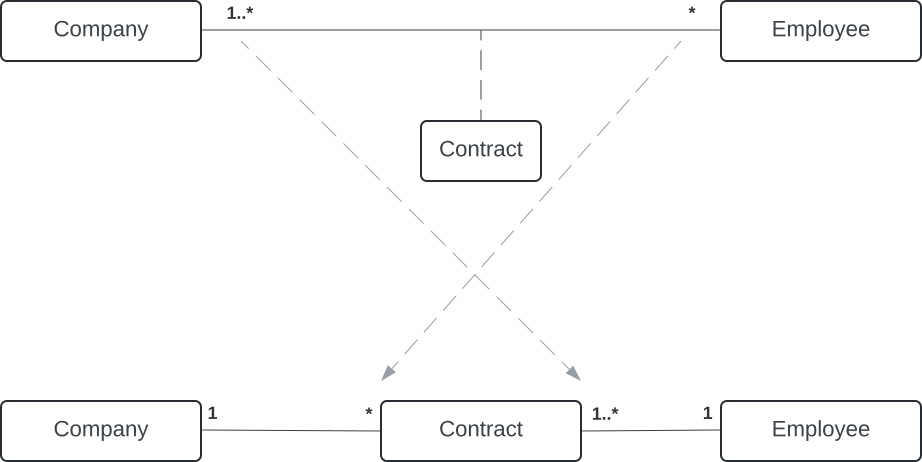
\includegraphics[scale=0.4]{part three/Klassendiagramme - Erweiterte Konzepte und Paketdiagramme/img/assoziationsklasse}
    \caption{Darstellung einer Assoziation mit Hilfe einer Assoziationsklasse (oben) sowie Transformation in gewöhnliche Assoziationen (unten). (Quelle: in Anlehnung an \cite[279, Abb. 4.4-11]{Oes05})}
    \label{fig:assoziationsklasse-cc}
\end{figure}

\clearpage


\section{Sequenzdiagramme}

\begin{tcolorbox}[title=Sequenzdiagramme]
    \textbf{Sequenzdiagramme} stellen Verhalten auf der Ebene einer Interaktion dar.\\
    In der Phase des Klassendesigns werden die Teilnehmer der Interaktionen bestimmt, weshalb Sequenzdiagramme oft in dieser Phase genutzt werden.\\
    In der \textbf{Analysephase} können Sequenzdiagramme eingesetzt werden, um die Kommunikation der bis dahin ausgemachten \textbf{Geschäftsobjekte} zu modellieren, oder um \textbf{Anwendungsfälle} weiter zu spezifizieren.
\end{tcolorbox}
\clearpage

\section{Aggregation}

\begin{tcolorbox}[title=Aggregation]
    Eine \textbf{Aggregation} ist in ihrer \semantischen Aussage unscharf (vgl.~\cite[40]{Buh09}).\\
    Sie beschreibt eine \textit{Ganzes}-\textit{Teile}-Beziehung, aber die \textit{Teile} können zu mehreren verschiedenen \textit{Ganzen} gehören.\\
    Außerdem kann ein Teil dem \textit{Ganzen} jederzeit wieder entnommen werden und das \textit{Ganze} ist nicht verantwortlich für das Erstellen der \textit{Teile}, weshalb Implementierungen beim Hinzufügen von Teilen oft schon fertige Objekte erwarten, die jeweils eines der \textit{Teile} repräsentieren.\\
    Aggregationsbeziehungen werden durch eine nicht-gefüllte Raute an der Seite der Klasse, die das Ganze repräsentiert, dargestellt.
\end{tcolorbox}
\clearpage

\section{Komposition}

\begin{tcolorbox}[title=Komposition]
    Bei einer \textbf{Komposition} handelt es sich um eine \textit{Ganzes}-\textit{Teile}-Beziehung, bei der das \textit{Ganze} verantwortlich für die Erstellung und Beseitigung der \textit{Teile} ist.
    Außerdem sind die \textit{Teile} an die \textbf{Existenz} des \textit{Ganzen} gebunden.\\
    \textit{Teile} gehören immer zu \textit{genau einem} \textit{Ganzen}.\\
    Eine Komposition wird dargestellt durch eine gefüllte Raute an der Klassenbox, die das \textit{Ganze} repräsentiert.
\end{tcolorbox}
\clearpage

\section{Paketdiagramm}

\begin{tcolorbox}[title=Komposition]
    \textbf{Paketdiagramme} zeigen Pakete und ihre Abhängigkeiten und werden in frühen Designphasen genutzt, um Strukturen (großer Systeme) aufzuzeigen.\\

    \noindent
    Elemente sollten so in Paketen gruppiert werden, dass ihr \textbf{funktionaler Zusammenhalt} (\textit{Kohäsion}, s. Abschnitt~\ref{subsec:hohe-kohasion}) klar wird.\\
    Hierdurch kann vermieden werden, dass Änderungen einer Klasse eines Paketes auch Änderungen außerhalb des Paketes erfordern.\\
    Außerdem erhöht sich die Wahrscheinlichkeit, dass einzelne Pakete als solche in anderen Projekten wiederverwendet werden können.\\

    \noindent
    In Paketdiagrammen können Beziehungen über folgende Schlüsselwörter deutlich gemacht werden:

    \begin{itemize}
        \item \guillemotleft import\guillemotright
        \item[] $\rightarrow$ \textbf{public-Import} zwischen Quell- und Zielpaket; Quellpaket kann die öffentlichen Elemente des Zielpaketes unter Verwendung des unqualifizierten und des qualifizierten Namens verwenden; die importierten Elemente sind auch für Pakete sichtbar, die das Quellpaket importieren
        \item \guillemotleft access\guillemotright
        \item[] $\rightarrow$ \textbf{privater Import} zwischen Quell- und Zielpaket; Zugriff auf Elemente des importierten Paketes ohne qualifizierenden Namen möglich; der Import eines Paketes in \textbf{Java} entspricht der \guillemotleft access\guillemotright-Beziehung
        \item \guillemotleft merge\guillemotright
        \item[] $\rightarrow$ Bei einem \textbf{merge} werden Elemente eines Zielpaketes in das Quellpaket
   \end{itemize}
\end{tcolorbox}
\clearpage

\section{Anwendungsfalldiagramm}

\begin{tcolorbox}[title=Anwendungsfalldiagramm]
    Die \textbf{Anwendungsfallanalyse} wird im Rahmen der \textbf{Anforderungsspezifikation} eingesetzt.\\

    \noindent
    Anwendungsfalldiagramme sind das am häufigsten eingesetzte Mittel zur Aufnahme und Darstellung von \textbf{Anforderungen}.\\
    Sie beschreiben selbst kein Verhalten und keine Abläufe, sondern zeigen nur die Zusammenhänge der an Anwendungsfällen beteiligten Modellelemente und sind somit ein Hilfsmittel zur Anforderungsermittlung und Verwaltung.\\

    \noindent
    Zu den wichtigsten Schritten einer Anwendungsfallanalyse gehören:
    \begin{enumerate}
        \item Akteure identifizieren
        \item Anwendungsfälle identifizieren
        \item Beschreiben der Akteure und Anwendungsfälle
        \item Identifizieren von \textit{Schlüsselobjekten}, die das System verwaltet
        \item Identifizieren der wichtigsten Anwendungsfälle (Priorisierung)
        \item detailliertere Beschreibung der Anwendungsfälle
        \item Strukturierung des Anwendungsfalldiagramms
    \end{enumerate}

    \noindent
    Anwendungsfälle beschreiben das \textbf{Szenario} der Nutzung, und nicht Features des Systems.
\end{tcolorbox}

\clearpage

\input{chapters/Anhang/CheatSheets/SE3/Aktivitätsdiagramm}
\clearpage

\section{Zustandsautomat}

\begin{tcolorbox}[title=Zustandsautomat]
    Mit \textbf{Zustandsautomaten} kann das \textit{Verhalten} von Systemen modelliert werden, wobei die \textit{Reaktionen} des Systems im Mittelpunkt stehen, und nicht die \textit{Aktionen}, wie bspw. bei den \textbf{Aktivitätsdiagrammen}.\\

    \noindent
        Ein \textbf{Zustandsautomat} kann den \textit{Lebensweg} eines Objektes modellieren, weshalb Zustandsautomaten oft im \textbf{Entwurf} als Ergänzung zu den \textbf{Klassendiagrammen} eingesetzt werden.
\end{tcolorbox}

\begin{figure}
    \centering
    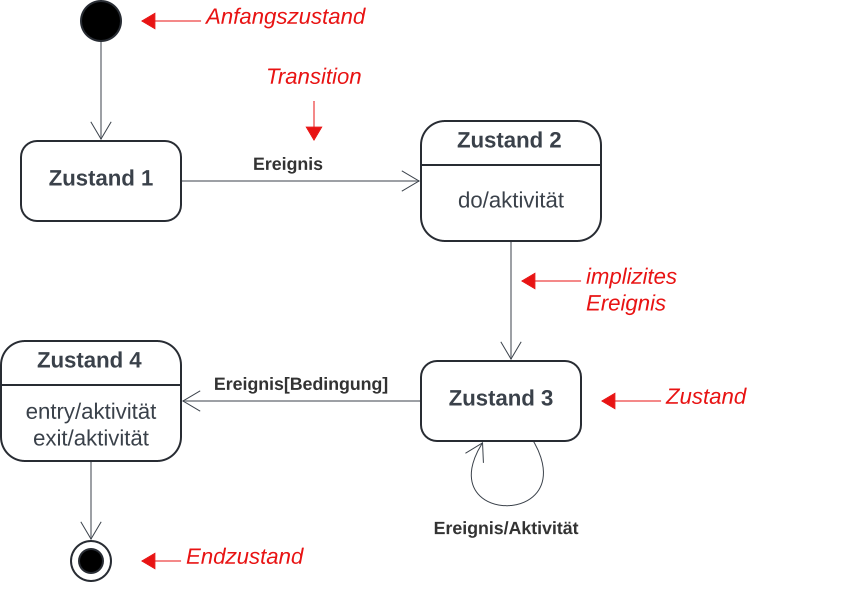
\includegraphics[scale=0.4]{part three/Zustandsautomaten/img/statechartdiagramnotation}
    \caption{Elemente eines einfachen Zustandsautomaten. Eine Transitionen wird durch ein \textbf{Ereignis} ausgelöst, das ein \textit{Signal}, ein \textit{Operationsaufruf} oder auch eine bestimmte \textit{Attributänderung} sein kann. (Quelle: in Anlehnung an \cite[90, Abb. 2.11-6]{Bal05})}
    \label{fig:statechartdiagramnotation-cc}
\end{figure}

\begin{minted}[fontsize=\small]{java}
// Beispiel für eine Implementierung eines
// Parkscheinautomaten als Zustandsautomat in Java
class Parkscheinautomat {

  // zustände
  private final int BEREIT = 0;
  private final int ZAHLUNG = 1;
  private final int ABBRUCH = 2;
  private final int BELEG   = 3;

  // Zustand; wird initial beim Starten
  // des Automaten gesetzt
  private int zustand;

  // Methoden lösen Aktionen beim Eintritt
  // in die jeweiligen Zustände aus
  private int zahlung() {
    // verarbeiten
    // danach neuen Zustand zurückliefern...
    ...
    return BEREIT;
  }

   ...

  private void bereit() {
    while (true) {
      // eingabe überprüfen und
      // ggf. Zustandswechsel auslösen:
      // Zustand als Attribut setzen
      ...
    }
  }

  public void start() {
    zustand = BEREIT;

    while(true) {
      switch (zustand) {
        case BEREIT:
          zustand = bereit();
        // ... weiteres Verhalten
        ...
      }
    }
  }
}
\end{minted}
\clearpage
	

\section{Inhalt SE3}

\section*{1. Übersicht UML}

\subsection*{Lernziele}
\begin{itemize}
    \item einen Einblick in den Sprachaufbau der UML 2.0 gewinnen
    \item einen Überblick über die Diagramme der UML 2.0 und deren Zweck haben
\end{itemize}

\subsection*{Zusammenfassung}
\begin{itemize}
    \item Die \textbf{UML} ist eine weit verbreitete Modellierungssprache zur Modellierung objektorientierter Softwaresysteme.
    \item Die UML 2.0 Spezifikation besteht aus vier Teilen:
    \begin{enumerate}
        \item \textbf{Superstructure}: Diagrammtypen
        \item \textbf{Infrastructure}: Modellierungskonzepte
        \item \textbf{OCL}: formale Sprache zur Formulierung von Einschränkungen
        \item \textbf{Diagram Interchange}: Austauschformate
    \end{enumerate}
    \item Die UML kann im \textbf{Sketching} oder \textbf{Blueprint Modus} eingesetzt werden, oder als Grundlage für \textbf{automatische Codegenerierung}
    \item Die UML ist an keinen speziellen Entwicklungsprozess gebunden
\end{itemize}

\section*{2. Klassendiagramme}

\subsection*{Lernziele}
\begin{itemize}
    \item wissen, wie Klassendiagramme im Entwicklungsprozess eingesetzt werden
    \item Klassendiagramme für Analyse- und Designentscheidungen einsetzen können
    \item die wichtigsten Modellierungskonzepte kennen
    \item sinnvolle Klassendiagramme erstellen und Java-Implementierungen ableiten können
    \item Klassendiagramme aus Java Quellcode erzeugen können
\end{itemize}

\subsection*{Zusammenfassung}

\begin{itemize}
    \item \textbf{Klassendiagramme} dienen zur \textbf{strukturellen Darstellung} von Softwaresystemen
    \item hierbei werden Klassen und \textbf{Beziehungen} zwischen Klassen dargestellt
    \item Properties können durch die \textbf{Attribut}- oder \textbf{Assoziationsnotation} modelliert werden
    \item Operationen werden als separate Zeile in ihrem Compartment dargestellt
    \item im Klassendiagramm können auch \textbf{Generalisierungsbeziehungen} modelliert werden
    \item \textbf{Abhängigkeitsbeziehungen} drücken ein Verhältnis zwischen \textbf{Client} und \textbf{Supplier} aus
\end{itemize}

\section*{3. Objektorientierter Entwurf}

\subsection*{Lernziele}
\begin{itemize}
    \item das Wesen einer Interaktion kennen
    \item wissen, wie Sequenzdiagramme im Entwicklungsprozess eingesetzt werden
    \item Sequenzdiagramme für Analyse- und Designentscheidungen sowie zur Darstellung von Kontrollflüssen einsetzen können
    \item die wichtigsten Modellierungskonzepte kennen
    \item sinnvolle Sequenzdiagramme erstellen und Java-Implementierungen ableiten können
    \item Sequenzdiagramme aus Java Quellcode erzeugen können
\end{itemize}

\subsection*{Zusammenfassung}

\begin{itemize}
    \item Sequenzdiagramme sind \textbf{Verhaltensdiagramme}
    und können im gesamten Entwicklungszyklus zur Modellierung von Interaktionen angewendet werden
    \item Interaktionen bestehen im Wesentlichen aus dem Nachrichtenaustausch zwischen verschiedenen Kommunikationspartnern
    \item in den meisten Fällen wird die Kommunikation von Objekten von Klassen modelliert, aber es können auch Teilnehmer auf anderen Ebenen modelliert werden
    \item gewöhnlich gibt ein Sequenzdiagramm einen \textbf{Anwendungsfall} (\textit{Szenario}) wieder
    \item sie dienen nicht dazu, um Zustandsänderungen darzustellen (hierfür werden Zustandsdiagramme verwendet)
    \item Sequenzdiagramme sind \textit{nicht} gut geeignet für die Darstellung von
    \begin{itemize}
        \item nebenläufigem Verhalten (\textit{asynchrone} Nachrichten, \textit{kombiniertes Fragment})
        \item Schleifen und alternativem Verhalten (\textit{kombinierte Fragmente})
        \item[] $\rightarrow$  für beide Fälle sind \textbf{Aktivitätsdiagramme} besser geeignet
    \end{itemize}
\end{itemize}

\section*{4. Klassendiagramme - Erweiterte Konzepte und Paketdiagramme}

\subsection*{Lernziele}
\begin{itemize}
    \item erweiterte Modellierungskonzepte in Klassendiagrammen für den Detailentwurf von Systemen kennen
    \item die Konsequenzen dieser Konzepte in der Implementierung kennen
    \item wissen, wie Paketdiagramme im Entwicklungsprozess eingesetzt werden
    \item die Modellierungskonzepte in Paketdiagrammen kennen
    \item anhand von Paketdiagrammen Software-Architekturen gestalten und bewerten können
\end{itemize}

\subsection*{Zusammenfassung}

\begin{itemize}
    \item Die vorgestellten erweiterten Konzepte werden vor allem im \textbf{Feinentwurf} von Klassenstrukturen eingesetzt.
    \item Generell gilt, dass die Spezifikationen von Objekten und Properties nur so detailliert ausgeführt werden sollen, wie nötig: Sind Details für das Verständnis unnötig, sollte darauf verzichtet werden.
    \item \textbf{Generalisierungsbeziehungen} sollten grundsätzlich modelliert werden.
    \item Ist eine \textbf{Komposition} statt einer Generalisierung für den Sachverhalt möglich, sollte diese verwendet werden: ``Favor object composition over inheritance.`` (\cite[19 f.]{GHJV94})
    \item \textbf{Kompositionsbeziehungen} geben eindeutige Impulse für eine Implementierung, \textbf{Aggregationsbeziehungen} sind in ihrer semantischen Aussage nicht sehr eindeutig
    \item \textbf{Assoziationsklassen} sind in ihrer frühen Designphase empfehlenswert, die Realisierung (mit {bspw.} Java) erfordert aber eine Transformation in eine volle Klasse, wobei die Multiplizitäten angepasst werden müssen
    \item Elemente können in \textbf{Paketen} zusamengefasst und unter einem gemeinsamen Namensraum gruppiert werden
\end{itemize}

\section*{4. Anwendungsfalldiagramm (Use-Case-Diagramm)}

\subsection*{Lernziele}
\begin{itemize}
    \item wissen, wie die Anwendungsfallanalyse im Rahmen der Anforderungsspezifikation eingesetzt wird
    \item Prozessschritte der Anwendungsfallanalyse beherrschen
    \item die wichtigsten Modellierungskonzepte in Anwendungsfalldiagrammen kennen
    \item den Aufbau einer Anwendungsfallbeschreibung kennen
\end{itemize}

\subsection*{Zusammenfassung}

\begin{itemize}
    \item \textbf{Anwendungsfalldiagramme} besitzen eine einfache Notation, um \textbf{Akteure} und \textbf{Anwendungsfälle} eines \textbf{Systems} grafisch darzustellen
    \item auf Basis eines Anwendungsfalldiagramms lässt sich ermitteln, ob die Anwendungsfälle gewünschtes Verhalten realisieren bzw. Beziehungen zu einem oder mehreren Akteuren haben
    \item Anwendungsfälle und Akteure \textit{müssen} zusätzlich textlich beschrieben werden
\end{itemize}

\section*{5. Aktivitätsdiagramme}

\subsection*{Lernziele}
\begin{itemize}
    \item wissen, wie Aktivitätsdiagramme im Rahmen der Verhaltensanalyse in verschiedenen Prozessphasen eingesetzt werden können
    \item die wichtigsten Modellierungskonzepte in Aktivitätsdiagrammen kennen
    \item Aktivitätsdiagramme interpretieren, erstellen und implementieren können
\end{itemize}

\subsection*{Zusammenfassung}

\begin{itemize}
    \item \textbf{Aktivitätsdiagramme} gehören zu den \textbf{Verhaltensdiagrammen} und können im \textit{gesamten} \textbf{Entwicklungsprozess} eingesetzt werden
    \item durch ein Aktivitätsdiagramm kann gezeigt werden, wie \textbf{Verhalten} realisiert wird
    \item es können mehrere \textbf{Aktivitäten} dargestellt werden
    \item \textbf{Aktivitätskanten} und \textbf{Aktivitätsknoten} werden zur Beschreibung von Verhalten verwendet
\end{itemize}

\section*{5. Zustandsautomaten}

\subsection*{Lernziele}
\begin{itemize}
    \item wissen, wie Zustandsdiagramme im Rahmen der Verhaltensanalyse einzelner Objekte eingesetzt werden können
    \item die wichtigsten Modellierungskonzepte in Zustandsdiagrammen kennen
    \item Zustandsdiagramme interpretieren, erstellen und implementieren können
\end{itemize}

\subsection*{Zusammenfassung}

\begin{itemize}
    \item Das \textbf{Zustandsdiagramm} gehört wie das \textbf{Aktivitätsdiagramm} zu den \textbf{Verhaltensdiagrammen}.
    \item Ein Zustandsdiagramm zeigt den \textbf{Lebensweg} eines \textbf{Objektes}.
    \item \textbf{Attributwerte} bestimmen den Zustand eines Objektes.
    \item \textbf{Transitionen} zwischen Zuständen werden durch \textbf{Guards} und \textbf{Events} gesteuert.
    \item Während der Transitionen können \textbf{Effekte} (\textit{Aktivitäten}) realisiert werden.
    \item Die Modellierung \textbf{zusammengesetzter Zustände} ist ebenfalls möglich.
    \item Für die Darstellung \textbf{paralleler} oder  \textbf{konkurrierender} Abläufe können \textbf{Regionen} modelliert werden.
\end{itemize}
\clearpage


\section{UML Modellierung}

\begin{tcolorbox}[title=UML Modellierung]
    \textbf{Modelle} haben die Aufgabe, den Bezug zum Original (Programm, Softwaresystem) herzustellen, sowie zu der \textit{Anwendungsumgebung}.\\
    Ein \textbf{Modell} enthält alle \textbf{Modellelemente}, die zur Beschreibung eines Softwaresystems nötig sind.\\

    \noindent
    Ein \textbf{Modellelement} wird als Element in einem UML Modell von einem Benutzer erstellt und auf verschiedenen \textbf{Diagrammen} (Struktur-/Verhaltensdiagrammen) platziert, und wird durch die \textbf{UML Modellierungskonzepte} als Metaklasse des \textbf{Metamodells} der UML beschrieben: \textbf{Modellelemente} werden aus Modellierungskonzepten instanziiert.\\

    \noindent
       Das \textbf{UML Metamodell} regelt, in welchem Zusammenhang \textbf{UML Modellierungskonzepte} in Modellen auftreten dürfen, und welche Eigenschaften und Beziehungen zu anderen Sprachelementen zulässig sind.\\

       \noindent
       Die im \textbf{Metamodell} verwendeten Erklärungen basieren auf einer abstrakten Syntax, für deren Beschreibung eine Untermenge (\textit{Klassendiagramme}) der UML verwendet wird.\\
        Die \textbf{Semantik} der Modellierungskonzepte wird textlich beschrieben, zur Formalisierung von Regeln für die syntaktische Korrektheit wird die \textbf{OCL} (\textit{Object Constraint Language}) verwendet.
\end{tcolorbox}

\begin{figure}
    \centering
    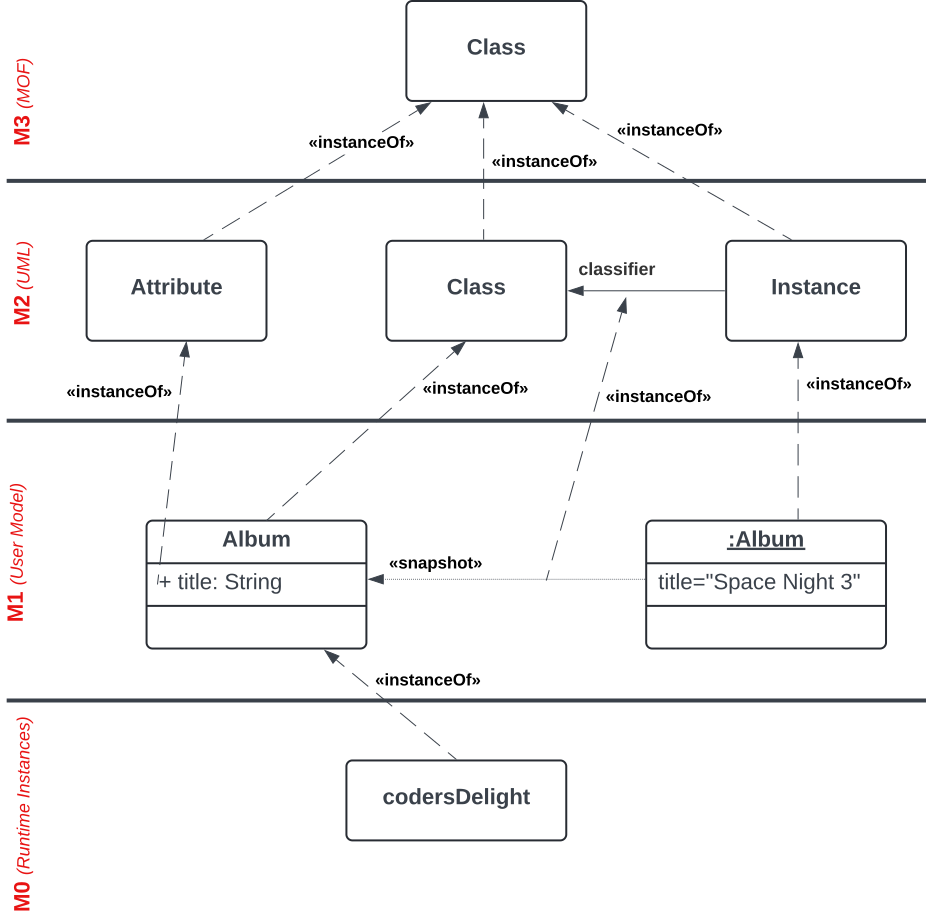
\includegraphics[scale=0.4]{part three/Einführung/img/metamodel}
    \caption{Beispiel für die verschiedenen Schichten der Metamodell Hierarchie.
        In der original Abbildung sind die Pfeilspitzen offen. (Quelle: in Anlehnung an S. 20, Figure 7.8, \url{https://www.omg.org/spec/UML/2.4.1/Infrastructure/PDF}, abgerufen 01.05.2024}
    \label{fig:metamodel-cc}
\end{figure}

\clearpage


\section{Strukturdiagramme}

\begin{tcolorbox}[title=Strukturdiagramme]
    In den \textbf{Strukturdiagrammen} werden \textbf{statische Strukturaspekte} eines Systems betrachtet.
    Für eine Systemmodellierung können alle dieser 6 Diagramme verwendet werden.

    \begin{itemize}
        \item \textbf{Klassendiagramm}: Das \textbf{Klassendiagramm} wird verwendet, um ein objektorientiertes System zu beschreiben.
        \item \textbf{Paketdiagramm}: Ein \textbf{Paketdiagramm} zeigt die Pakete eines Systems und deren Beziehungen.
        \item \textbf{Komponentendiagramm}: Stellt Komponenten oder auch \textit{Subsysteme} mit definierten Interfaces dar, um bspw. \textbf{Architekturdesign} darzustellen.
        \item \textbf{Verteilungsdiagramm}: Beschreibt eine Menge von Knoten, die die \textit{Ausführungsarchitektur} eines Systems definieren können, wobei Knoten i.d.R. \textit{Geräte} oder \textit{Softwareablaufumgebungen repräsentieren}.
        \item \textbf{Kompositionsstrukturdiagramm}: Stellt die \textbf{Komposition} von \textit{Systemstrukturen} (Klassen, Komponenten, Gesamtsystem) in einem bestimmten \textit{Kontext} mit einem bestimmten \textit{Ziel} dar (vgl. \cite[9]{Buh09}).
        \item \textbf{Objektdiagramm}: Momentaufnahme eines Systems zu genau einem \textit{Zeitpukt} während der Ausführung
    \end{itemize}

\end{tcolorbox}
\clearpage

\section{Verhaltensdiagramme}

\begin{tcolorbox}[title=Verhaltensdiagramme]
    \textbf{Verhaltensdiagramme} stellen \textit{Dynamik}, \textit{interne Abläufe} und das \textit{Zusammenspiel} der Systemteile dar, um eine Spezifikation zu vervollständigen.

    \begin{itemize}
        \item \textbf{Anwendungsfalldiagramm}: Dienen zur \textit{Spezifizierung} und \textit{Formalisierung} von \textit{Systemanforderungen}, unter Berücksichtigung von \textbf{Akteuren}, \textbf{Systemen} und \textbf{Anwendungsfällen}
        \item \textbf{Zustandsdiagramm}: Auch \textbf{Zustandsautomaten}; zeigen für ein einzelnes Objekt Zustandsänderungen während der Lebenszeit
        \item \textbf{Aktivitätsdiagramme}: Werden zur Modellierung von \textit{Kontroll}- oder \textit{Objektflüssen} oder zur Darstellung von \textit{Programmlogik} genutzt.
        \item \textbf{Interaktionsdiagramme}: Stellen das Zusammenspiel mehrerer Kommunikationspartner dar.
        Es gibt unterschiedliche Typen von Interaktionsdiagrammen, die Interaktionen auf verschiedenen \textit{Abstraktionsebenen} modellieren:
        \begin{itemize}
            \item \textbf{Sequenzdiagramm}: Zeigt den Verlauf einer Interaktion in zwei Dimensionen, \textit{Kommunikationspartner} und die Nachrichten in ihrer \textit{zeitlichen Abfolge}
            \item \textbf{Kommunikationsdiagramm}: hebt die Kommunikationsbeziehungen zwischen den Partnern hervor
            \item \textbf{Timing Diagramm}: hebt die zeitlichen Aspekte einer Interaktion hervor
            \item \textbf{Interaktionsüberblickdiagramm}: Spezialfall des \textbf{Aktivitätsdiagramms} - statt Aktionen und Aktivitäten können das \textbf{Sequenz}-, \textbf{Kommunikations}- und das \textbf{Timing}-Diagramm als Knoten verwendet werden.
        \end{itemize}
        Alle verwenden dieselben Grundelemente: \textit{Lebenslinien} der Akteure und Nachrichten, die zwischen diesen ausgetauscht werden.
    \end{itemize}
\end{tcolorbox}

\clearpage


\section{Klassendiagramm}

\begin{tcolorbox}[title=Klassendiagramm]
    Das \textbf{Klassendiagramm} beschreibt die Klassen eines Systems und die statischen Beziehungen zwischen ihnen.\\
    Sie werden in Form von Domainklassen bei der \textbf{Analyse} und als detaillierte Entwürfe von Systemklassen als \textit{Blueprint} im \textbf{gesamten Entwicklungsprozess} eingesetzt.

\end{tcolorbox}
\clearpage


\section{Assoziationsklasse (Attributierte Assoziation)}

\begin{tcolorbox}[title=Assoziationsklasse (Attributierte Assoziation)]
Eine \textbf{Assoziationsklasse} erlaubt das Hinzufügen von Operationen und Attributen zu einer Assoziation (\cite[43]{Buh09}).\\
Assoziationsklassen werden in der \textbf{Analyse} in Modellen verwendet und in dem \textbf{Entwurf} in eigenständige Klassen transformiert.\\

\noindent
Assoziationsklassen werden in der \textbf{Analyse} in Modellen verwendet und in dem \textbf{Entwurf} in eigenständige Klassen transformiert.

\blockquote[{\cite[277]{Oes05}}]{
    Eine attributierte Assoziation ist immer dann nahe liegend, wenn Attribute oder Operationen gefunden werden, die weder der einen noch der anderen Klasse zugeordnet werden können, weil sie nämlich Eigenschaften der Beziehung selbst sind.
}.\\

Bei einer attributierten Assoziation dürfen zwei beteiligte Objekte maximal nur eine Beziehung zueinander haben (vgl.~\cite[277]{Oes05})\footnote{
    \textit{Ostereich} führt dies ebenda auf Seite 278 weiter aus, in dem er beschreibt, wie eine attributierte Assoziation für ein \textit{Beschäftigtenverhältnis} zwischen \textit{Mitarbeiter} und \textit{Unternehmen} modelliert wird. Dabei wird davon ausgegangen, dass ein \textit{Mitarbeiter} nur über \textit{ein} Arbeitsverhältnis mit einem \textit{Unternehmen} in Beziehung stehen kann. Bestehen mehrere Arbeitsverhältnisse (\textit{Mitarbeiter} hat zu unterschiedlichen Zeitpunkten für das \textit{Unternehmen} gearbeitet), kann die attributierte Assoziation nicht verwendet werden.\\

\noindent
Wird eine attributierte Assoziation in eine gewöhnliche Assoziation transformiert, muss darauf geachtet werden, die Multiplizitäten richtig zu setzen (s. Abbildung~\ref{fig:assoziationsklasse}).
\end{tcolorbox}

\begin{figure}
    \centering
    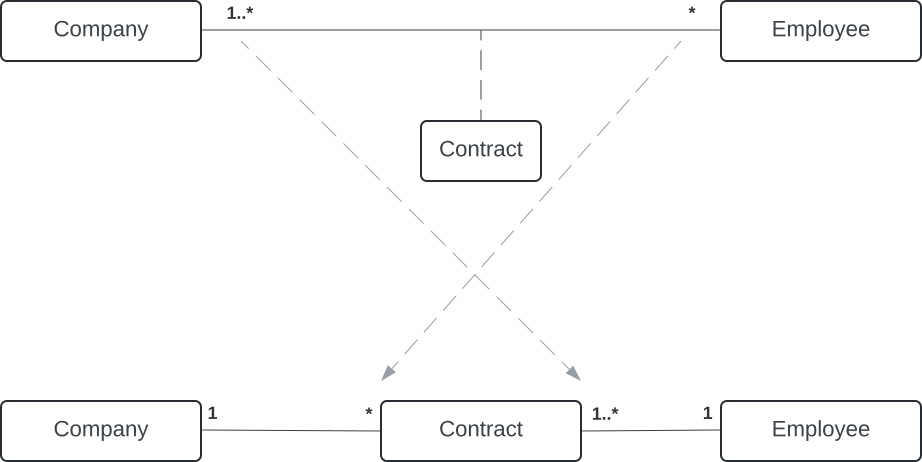
\includegraphics[scale=0.4]{part three/Klassendiagramme - Erweiterte Konzepte und Paketdiagramme/img/assoziationsklasse}
    \caption{Darstellung einer Assoziation mit Hilfe einer Assoziationsklasse (oben) sowie Transformation in gewöhnliche Assoziationen (unten). (Quelle: in Anlehnung an \cite[279, Abb. 4.4-11]{Oes05})}
    \label{fig:assoziationsklasse-cc}
\end{figure}

\clearpage


\section{Sequenzdiagramme}

\begin{tcolorbox}[title=Sequenzdiagramme]
    \textbf{Sequenzdiagramme} stellen Verhalten auf der Ebene einer Interaktion dar.\\
    In der Phase des Klassendesigns werden die Teilnehmer der Interaktionen bestimmt, weshalb Sequenzdiagramme oft in dieser Phase genutzt werden.\\
    In der \textbf{Analysephase} können Sequenzdiagramme eingesetzt werden, um die Kommunikation der bis dahin ausgemachten \textbf{Geschäftsobjekte} zu modellieren, oder um \textbf{Anwendungsfälle} weiter zu spezifizieren.
\end{tcolorbox}
\clearpage

\section{Aggregation}

\begin{tcolorbox}[title=Aggregation]
    Eine \textbf{Aggregation} ist in ihrer \semantischen Aussage unscharf (vgl.~\cite[40]{Buh09}).\\
    Sie beschreibt eine \textit{Ganzes}-\textit{Teile}-Beziehung, aber die \textit{Teile} können zu mehreren verschiedenen \textit{Ganzen} gehören.\\
    Außerdem kann ein Teil dem \textit{Ganzen} jederzeit wieder entnommen werden und das \textit{Ganze} ist nicht verantwortlich für das Erstellen der \textit{Teile}, weshalb Implementierungen beim Hinzufügen von Teilen oft schon fertige Objekte erwarten, die jeweils eines der \textit{Teile} repräsentieren.\\
    Aggregationsbeziehungen werden durch eine nicht-gefüllte Raute an der Seite der Klasse, die das Ganze repräsentiert, dargestellt.
\end{tcolorbox}
\clearpage

\section{Komposition}

\begin{tcolorbox}[title=Komposition]
    Bei einer \textbf{Komposition} handelt es sich um eine \textit{Ganzes}-\textit{Teile}-Beziehung, bei der das \textit{Ganze} verantwortlich für die Erstellung und Beseitigung der \textit{Teile} ist.
    Außerdem sind die \textit{Teile} an die \textbf{Existenz} des \textit{Ganzen} gebunden.\\
    \textit{Teile} gehören immer zu \textit{genau einem} \textit{Ganzen}.\\
    Eine Komposition wird dargestellt durch eine gefüllte Raute an der Klassenbox, die das \textit{Ganze} repräsentiert.
\end{tcolorbox}
\clearpage

\section{Paketdiagramm}

\begin{tcolorbox}[title=Komposition]
    \textbf{Paketdiagramme} zeigen Pakete und ihre Abhängigkeiten und werden in frühen Designphasen genutzt, um Strukturen (großer Systeme) aufzuzeigen.\\

    \noindent
    Elemente sollten so in Paketen gruppiert werden, dass ihr \textbf{funktionaler Zusammenhalt} (\textit{Kohäsion}, s. Abschnitt~\ref{subsec:hohe-kohasion}) klar wird.\\
    Hierdurch kann vermieden werden, dass Änderungen einer Klasse eines Paketes auch Änderungen außerhalb des Paketes erfordern.\\
    Außerdem erhöht sich die Wahrscheinlichkeit, dass einzelne Pakete als solche in anderen Projekten wiederverwendet werden können.\\

    \noindent
    In Paketdiagrammen können Beziehungen über folgende Schlüsselwörter deutlich gemacht werden:

    \begin{itemize}
        \item \guillemotleft import\guillemotright
        \item[] $\rightarrow$ \textbf{public-Import} zwischen Quell- und Zielpaket; Quellpaket kann die öffentlichen Elemente des Zielpaketes unter Verwendung des unqualifizierten und des qualifizierten Namens verwenden; die importierten Elemente sind auch für Pakete sichtbar, die das Quellpaket importieren
        \item \guillemotleft access\guillemotright
        \item[] $\rightarrow$ \textbf{privater Import} zwischen Quell- und Zielpaket; Zugriff auf Elemente des importierten Paketes ohne qualifizierenden Namen möglich; der Import eines Paketes in \textbf{Java} entspricht der \guillemotleft access\guillemotright-Beziehung
        \item \guillemotleft merge\guillemotright
        \item[] $\rightarrow$ Bei einem \textbf{merge} werden Elemente eines Zielpaketes in das Quellpaket
   \end{itemize}
\end{tcolorbox}
\clearpage

\section{Anwendungsfalldiagramm}

\begin{tcolorbox}[title=Anwendungsfalldiagramm]
    Die \textbf{Anwendungsfallanalyse} wird im Rahmen der \textbf{Anforderungsspezifikation} eingesetzt.\\

    \noindent
    Anwendungsfalldiagramme sind das am häufigsten eingesetzte Mittel zur Aufnahme und Darstellung von \textbf{Anforderungen}.\\
    Sie beschreiben selbst kein Verhalten und keine Abläufe, sondern zeigen nur die Zusammenhänge der an Anwendungsfällen beteiligten Modellelemente und sind somit ein Hilfsmittel zur Anforderungsermittlung und Verwaltung.\\

    \noindent
    Zu den wichtigsten Schritten einer Anwendungsfallanalyse gehören:
    \begin{enumerate}
        \item Akteure identifizieren
        \item Anwendungsfälle identifizieren
        \item Beschreiben der Akteure und Anwendungsfälle
        \item Identifizieren von \textit{Schlüsselobjekten}, die das System verwaltet
        \item Identifizieren der wichtigsten Anwendungsfälle (Priorisierung)
        \item detailliertere Beschreibung der Anwendungsfälle
        \item Strukturierung des Anwendungsfalldiagramms
    \end{enumerate}

    \noindent
    Anwendungsfälle beschreiben das \textbf{Szenario} der Nutzung, und nicht Features des Systems.
\end{tcolorbox}

\clearpage

\input{chapters/Anhang/CheatSheets/SE3/Aktivitätsdiagramm}
\clearpage

\section{Zustandsautomat}

\begin{tcolorbox}[title=Zustandsautomat]
    Mit \textbf{Zustandsautomaten} kann das \textit{Verhalten} von Systemen modelliert werden, wobei die \textit{Reaktionen} des Systems im Mittelpunkt stehen, und nicht die \textit{Aktionen}, wie bspw. bei den \textbf{Aktivitätsdiagrammen}.\\

    \noindent
        Ein \textbf{Zustandsautomat} kann den \textit{Lebensweg} eines Objektes modellieren, weshalb Zustandsautomaten oft im \textbf{Entwurf} als Ergänzung zu den \textbf{Klassendiagrammen} eingesetzt werden.
\end{tcolorbox}

\begin{figure}
    \centering
    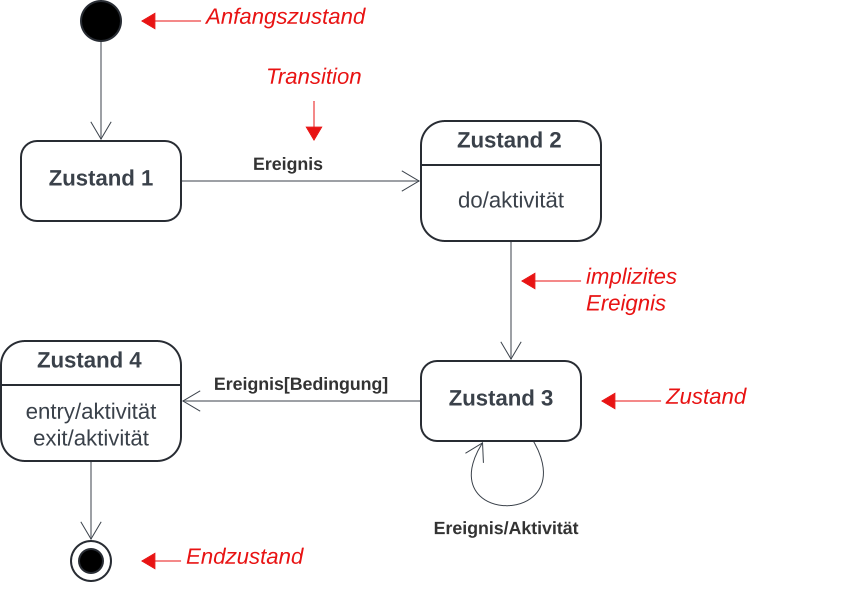
\includegraphics[scale=0.4]{part three/Zustandsautomaten/img/statechartdiagramnotation}
    \caption{Elemente eines einfachen Zustandsautomaten. Eine Transitionen wird durch ein \textbf{Ereignis} ausgelöst, das ein \textit{Signal}, ein \textit{Operationsaufruf} oder auch eine bestimmte \textit{Attributänderung} sein kann. (Quelle: in Anlehnung an \cite[90, Abb. 2.11-6]{Bal05})}
    \label{fig:statechartdiagramnotation-cc}
\end{figure}

\begin{minted}[fontsize=\small]{java}
// Beispiel für eine Implementierung eines
// Parkscheinautomaten als Zustandsautomat in Java
class Parkscheinautomat {

  // zustände
  private final int BEREIT = 0;
  private final int ZAHLUNG = 1;
  private final int ABBRUCH = 2;
  private final int BELEG   = 3;

  // Zustand; wird initial beim Starten
  // des Automaten gesetzt
  private int zustand;

  // Methoden lösen Aktionen beim Eintritt
  // in die jeweiligen Zustände aus
  private int zahlung() {
    // verarbeiten
    // danach neuen Zustand zurückliefern...
    ...
    return BEREIT;
  }

   ...

  private void bereit() {
    while (true) {
      // eingabe überprüfen und
      // ggf. Zustandswechsel auslösen:
      // Zustand als Attribut setzen
      ...
    }
  }

  public void start() {
    zustand = BEREIT;

    while(true) {
      switch (zustand) {
        case BEREIT:
          zustand = bereit();
        // ... weiteres Verhalten
        ...
      }
    }
  }
}
\end{minted}
\clearpage
	

\section{Inhalt SE3}

\section*{1. Übersicht UML}

\subsection*{Lernziele}
\begin{itemize}
    \item einen Einblick in den Sprachaufbau der UML 2.0 gewinnen
    \item einen Überblick über die Diagramme der UML 2.0 und deren Zweck haben
\end{itemize}

\subsection*{Zusammenfassung}
\begin{itemize}
    \item Die \textbf{UML} ist eine weit verbreitete Modellierungssprache zur Modellierung objektorientierter Softwaresysteme.
    \item Die UML 2.0 Spezifikation besteht aus vier Teilen:
    \begin{enumerate}
        \item \textbf{Superstructure}: Diagrammtypen
        \item \textbf{Infrastructure}: Modellierungskonzepte
        \item \textbf{OCL}: formale Sprache zur Formulierung von Einschränkungen
        \item \textbf{Diagram Interchange}: Austauschformate
    \end{enumerate}
    \item Die UML kann im \textbf{Sketching} oder \textbf{Blueprint Modus} eingesetzt werden, oder als Grundlage für \textbf{automatische Codegenerierung}
    \item Die UML ist an keinen speziellen Entwicklungsprozess gebunden
\end{itemize}

\section*{2. Klassendiagramme}

\subsection*{Lernziele}
\begin{itemize}
    \item wissen, wie Klassendiagramme im Entwicklungsprozess eingesetzt werden
    \item Klassendiagramme für Analyse- und Designentscheidungen einsetzen können
    \item die wichtigsten Modellierungskonzepte kennen
    \item sinnvolle Klassendiagramme erstellen und Java-Implementierungen ableiten können
    \item Klassendiagramme aus Java Quellcode erzeugen können
\end{itemize}

\subsection*{Zusammenfassung}

\begin{itemize}
    \item \textbf{Klassendiagramme} dienen zur \textbf{strukturellen Darstellung} von Softwaresystemen
    \item hierbei werden Klassen und \textbf{Beziehungen} zwischen Klassen dargestellt
    \item Properties können durch die \textbf{Attribut}- oder \textbf{Assoziationsnotation} modelliert werden
    \item Operationen werden als separate Zeile in ihrem Compartment dargestellt
    \item im Klassendiagramm können auch \textbf{Generalisierungsbeziehungen} modelliert werden
    \item \textbf{Abhängigkeitsbeziehungen} drücken ein Verhältnis zwischen \textbf{Client} und \textbf{Supplier} aus
\end{itemize}

\section*{3. Objektorientierter Entwurf}

\subsection*{Lernziele}
\begin{itemize}
    \item das Wesen einer Interaktion kennen
    \item wissen, wie Sequenzdiagramme im Entwicklungsprozess eingesetzt werden
    \item Sequenzdiagramme für Analyse- und Designentscheidungen sowie zur Darstellung von Kontrollflüssen einsetzen können
    \item die wichtigsten Modellierungskonzepte kennen
    \item sinnvolle Sequenzdiagramme erstellen und Java-Implementierungen ableiten können
    \item Sequenzdiagramme aus Java Quellcode erzeugen können
\end{itemize}

\subsection*{Zusammenfassung}

\begin{itemize}
    \item Sequenzdiagramme sind \textbf{Verhaltensdiagramme}
    und können im gesamten Entwicklungszyklus zur Modellierung von Interaktionen angewendet werden
    \item Interaktionen bestehen im Wesentlichen aus dem Nachrichtenaustausch zwischen verschiedenen Kommunikationspartnern
    \item in den meisten Fällen wird die Kommunikation von Objekten von Klassen modelliert, aber es können auch Teilnehmer auf anderen Ebenen modelliert werden
    \item gewöhnlich gibt ein Sequenzdiagramm einen \textbf{Anwendungsfall} (\textit{Szenario}) wieder
    \item sie dienen nicht dazu, um Zustandsänderungen darzustellen (hierfür werden Zustandsdiagramme verwendet)
    \item Sequenzdiagramme sind \textit{nicht} gut geeignet für die Darstellung von
    \begin{itemize}
        \item nebenläufigem Verhalten (\textit{asynchrone} Nachrichten, \textit{kombiniertes Fragment})
        \item Schleifen und alternativem Verhalten (\textit{kombinierte Fragmente})
        \item[] $\rightarrow$  für beide Fälle sind \textbf{Aktivitätsdiagramme} besser geeignet
    \end{itemize}
\end{itemize}

\section*{4. Klassendiagramme - Erweiterte Konzepte und Paketdiagramme}

\subsection*{Lernziele}
\begin{itemize}
    \item erweiterte Modellierungskonzepte in Klassendiagrammen für den Detailentwurf von Systemen kennen
    \item die Konsequenzen dieser Konzepte in der Implementierung kennen
    \item wissen, wie Paketdiagramme im Entwicklungsprozess eingesetzt werden
    \item die Modellierungskonzepte in Paketdiagrammen kennen
    \item anhand von Paketdiagrammen Software-Architekturen gestalten und bewerten können
\end{itemize}

\subsection*{Zusammenfassung}

\begin{itemize}
    \item Die vorgestellten erweiterten Konzepte werden vor allem im \textbf{Feinentwurf} von Klassenstrukturen eingesetzt.
    \item Generell gilt, dass die Spezifikationen von Objekten und Properties nur so detailliert ausgeführt werden sollen, wie nötig: Sind Details für das Verständnis unnötig, sollte darauf verzichtet werden.
    \item \textbf{Generalisierungsbeziehungen} sollten grundsätzlich modelliert werden.
    \item Ist eine \textbf{Komposition} statt einer Generalisierung für den Sachverhalt möglich, sollte diese verwendet werden: ``Favor object composition over inheritance.`` (\cite[19 f.]{GHJV94})
    \item \textbf{Kompositionsbeziehungen} geben eindeutige Impulse für eine Implementierung, \textbf{Aggregationsbeziehungen} sind in ihrer semantischen Aussage nicht sehr eindeutig
    \item \textbf{Assoziationsklassen} sind in ihrer frühen Designphase empfehlenswert, die Realisierung (mit {bspw.} Java) erfordert aber eine Transformation in eine volle Klasse, wobei die Multiplizitäten angepasst werden müssen
    \item Elemente können in \textbf{Paketen} zusamengefasst und unter einem gemeinsamen Namensraum gruppiert werden
\end{itemize}

\section*{4. Anwendungsfalldiagramm (Use-Case-Diagramm)}

\subsection*{Lernziele}
\begin{itemize}
    \item wissen, wie die Anwendungsfallanalyse im Rahmen der Anforderungsspezifikation eingesetzt wird
    \item Prozessschritte der Anwendungsfallanalyse beherrschen
    \item die wichtigsten Modellierungskonzepte in Anwendungsfalldiagrammen kennen
    \item den Aufbau einer Anwendungsfallbeschreibung kennen
\end{itemize}

\subsection*{Zusammenfassung}

\begin{itemize}
    \item \textbf{Anwendungsfalldiagramme} besitzen eine einfache Notation, um \textbf{Akteure} und \textbf{Anwendungsfälle} eines \textbf{Systems} grafisch darzustellen
    \item auf Basis eines Anwendungsfalldiagramms lässt sich ermitteln, ob die Anwendungsfälle gewünschtes Verhalten realisieren bzw. Beziehungen zu einem oder mehreren Akteuren haben
    \item Anwendungsfälle und Akteure \textit{müssen} zusätzlich textlich beschrieben werden
\end{itemize}

\section*{5. Aktivitätsdiagramme}

\subsection*{Lernziele}
\begin{itemize}
    \item wissen, wie Aktivitätsdiagramme im Rahmen der Verhaltensanalyse in verschiedenen Prozessphasen eingesetzt werden können
    \item die wichtigsten Modellierungskonzepte in Aktivitätsdiagrammen kennen
    \item Aktivitätsdiagramme interpretieren, erstellen und implementieren können
\end{itemize}

\subsection*{Zusammenfassung}

\begin{itemize}
    \item \textbf{Aktivitätsdiagramme} gehören zu den \textbf{Verhaltensdiagrammen} und können im \textit{gesamten} \textbf{Entwicklungsprozess} eingesetzt werden
    \item durch ein Aktivitätsdiagramm kann gezeigt werden, wie \textbf{Verhalten} realisiert wird
    \item es können mehrere \textbf{Aktivitäten} dargestellt werden
    \item \textbf{Aktivitätskanten} und \textbf{Aktivitätsknoten} werden zur Beschreibung von Verhalten verwendet
\end{itemize}

\section*{5. Zustandsautomaten}

\subsection*{Lernziele}
\begin{itemize}
    \item wissen, wie Zustandsdiagramme im Rahmen der Verhaltensanalyse einzelner Objekte eingesetzt werden können
    \item die wichtigsten Modellierungskonzepte in Zustandsdiagrammen kennen
    \item Zustandsdiagramme interpretieren, erstellen und implementieren können
\end{itemize}

\subsection*{Zusammenfassung}

\begin{itemize}
    \item Das \textbf{Zustandsdiagramm} gehört wie das \textbf{Aktivitätsdiagramm} zu den \textbf{Verhaltensdiagrammen}.
    \item Ein Zustandsdiagramm zeigt den \textbf{Lebensweg} eines \textbf{Objektes}.
    \item \textbf{Attributwerte} bestimmen den Zustand eines Objektes.
    \item \textbf{Transitionen} zwischen Zuständen werden durch \textbf{Guards} und \textbf{Events} gesteuert.
    \item Während der Transitionen können \textbf{Effekte} (\textit{Aktivitäten}) realisiert werden.
    \item Die Modellierung \textbf{zusammengesetzter Zustände} ist ebenfalls möglich.
    \item Für die Darstellung \textbf{paralleler} oder  \textbf{konkurrierender} Abläufe können \textbf{Regionen} modelliert werden.
\end{itemize}
\clearpage


\section{UML Modellierung}

\begin{tcolorbox}[title=UML Modellierung]
    \textbf{Modelle} haben die Aufgabe, den Bezug zum Original (Programm, Softwaresystem) herzustellen, sowie zu der \textit{Anwendungsumgebung}.\\
    Ein \textbf{Modell} enthält alle \textbf{Modellelemente}, die zur Beschreibung eines Softwaresystems nötig sind.\\

    \noindent
    Ein \textbf{Modellelement} wird als Element in einem UML Modell von einem Benutzer erstellt und auf verschiedenen \textbf{Diagrammen} (Struktur-/Verhaltensdiagrammen) platziert, und wird durch die \textbf{UML Modellierungskonzepte} als Metaklasse des \textbf{Metamodells} der UML beschrieben: \textbf{Modellelemente} werden aus Modellierungskonzepten instanziiert.\\

    \noindent
       Das \textbf{UML Metamodell} regelt, in welchem Zusammenhang \textbf{UML Modellierungskonzepte} in Modellen auftreten dürfen, und welche Eigenschaften und Beziehungen zu anderen Sprachelementen zulässig sind.\\

       \noindent
       Die im \textbf{Metamodell} verwendeten Erklärungen basieren auf einer abstrakten Syntax, für deren Beschreibung eine Untermenge (\textit{Klassendiagramme}) der UML verwendet wird.\\
        Die \textbf{Semantik} der Modellierungskonzepte wird textlich beschrieben, zur Formalisierung von Regeln für die syntaktische Korrektheit wird die \textbf{OCL} (\textit{Object Constraint Language}) verwendet.
\end{tcolorbox}

\begin{figure}
    \centering
    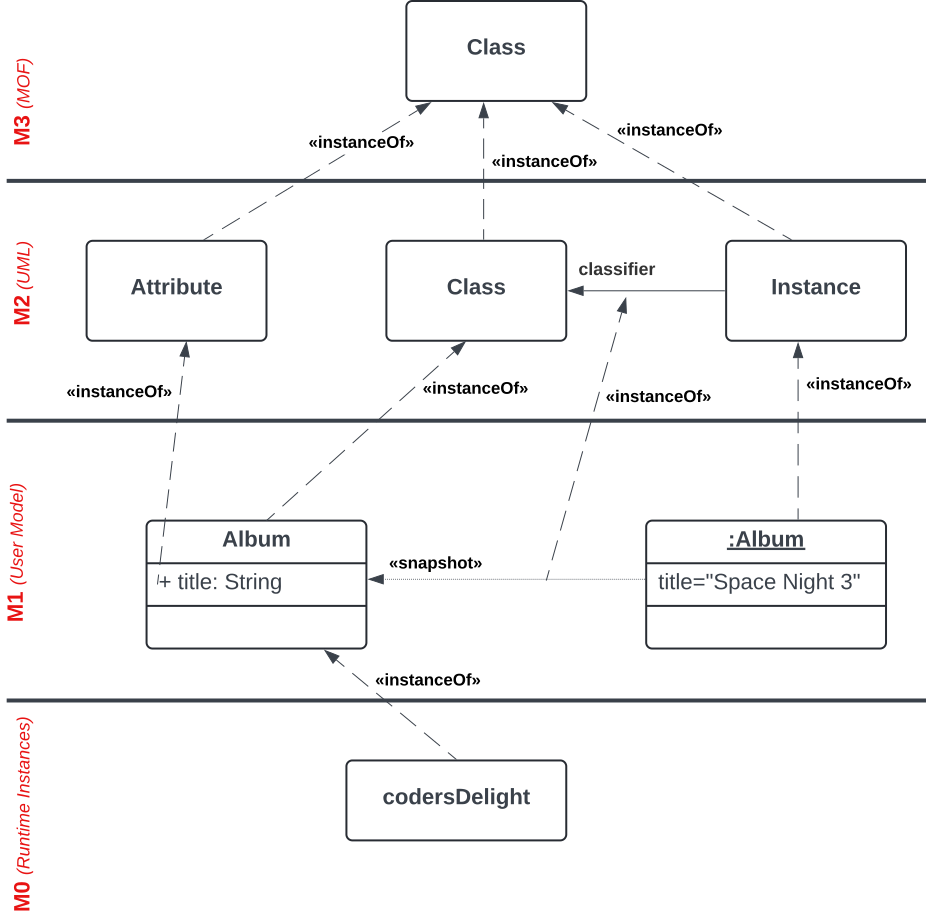
\includegraphics[scale=0.4]{part three/Einführung/img/metamodel}
    \caption{Beispiel für die verschiedenen Schichten der Metamodell Hierarchie.
        In der original Abbildung sind die Pfeilspitzen offen. (Quelle: in Anlehnung an S. 20, Figure 7.8, \url{https://www.omg.org/spec/UML/2.4.1/Infrastructure/PDF}, abgerufen 01.05.2024}
    \label{fig:metamodel-cc}
\end{figure}

\clearpage


\section{Strukturdiagramme}

\begin{tcolorbox}[title=Strukturdiagramme]
    In den \textbf{Strukturdiagrammen} werden \textbf{statische Strukturaspekte} eines Systems betrachtet.
    Für eine Systemmodellierung können alle dieser 6 Diagramme verwendet werden.

    \begin{itemize}
        \item \textbf{Klassendiagramm}: Das \textbf{Klassendiagramm} wird verwendet, um ein objektorientiertes System zu beschreiben.
        \item \textbf{Paketdiagramm}: Ein \textbf{Paketdiagramm} zeigt die Pakete eines Systems und deren Beziehungen.
        \item \textbf{Komponentendiagramm}: Stellt Komponenten oder auch \textit{Subsysteme} mit definierten Interfaces dar, um bspw. \textbf{Architekturdesign} darzustellen.
        \item \textbf{Verteilungsdiagramm}: Beschreibt eine Menge von Knoten, die die \textit{Ausführungsarchitektur} eines Systems definieren können, wobei Knoten i.d.R. \textit{Geräte} oder \textit{Softwareablaufumgebungen repräsentieren}.
        \item \textbf{Kompositionsstrukturdiagramm}: Stellt die \textbf{Komposition} von \textit{Systemstrukturen} (Klassen, Komponenten, Gesamtsystem) in einem bestimmten \textit{Kontext} mit einem bestimmten \textit{Ziel} dar (vgl. \cite[9]{Buh09}).
        \item \textbf{Objektdiagramm}: Momentaufnahme eines Systems zu genau einem \textit{Zeitpukt} während der Ausführung
    \end{itemize}

\end{tcolorbox}
\clearpage

\section{Verhaltensdiagramme}

\begin{tcolorbox}[title=Verhaltensdiagramme]
    \textbf{Verhaltensdiagramme} stellen \textit{Dynamik}, \textit{interne Abläufe} und das \textit{Zusammenspiel} der Systemteile dar, um eine Spezifikation zu vervollständigen.

    \begin{itemize}
        \item \textbf{Anwendungsfalldiagramm}: Dienen zur \textit{Spezifizierung} und \textit{Formalisierung} von \textit{Systemanforderungen}, unter Berücksichtigung von \textbf{Akteuren}, \textbf{Systemen} und \textbf{Anwendungsfällen}
        \item \textbf{Zustandsdiagramm}: Auch \textbf{Zustandsautomaten}; zeigen für ein einzelnes Objekt Zustandsänderungen während der Lebenszeit
        \item \textbf{Aktivitätsdiagramme}: Werden zur Modellierung von \textit{Kontroll}- oder \textit{Objektflüssen} oder zur Darstellung von \textit{Programmlogik} genutzt.
        \item \textbf{Interaktionsdiagramme}: Stellen das Zusammenspiel mehrerer Kommunikationspartner dar.
        Es gibt unterschiedliche Typen von Interaktionsdiagrammen, die Interaktionen auf verschiedenen \textit{Abstraktionsebenen} modellieren:
        \begin{itemize}
            \item \textbf{Sequenzdiagramm}: Zeigt den Verlauf einer Interaktion in zwei Dimensionen, \textit{Kommunikationspartner} und die Nachrichten in ihrer \textit{zeitlichen Abfolge}
            \item \textbf{Kommunikationsdiagramm}: hebt die Kommunikationsbeziehungen zwischen den Partnern hervor
            \item \textbf{Timing Diagramm}: hebt die zeitlichen Aspekte einer Interaktion hervor
            \item \textbf{Interaktionsüberblickdiagramm}: Spezialfall des \textbf{Aktivitätsdiagramms} - statt Aktionen und Aktivitäten können das \textbf{Sequenz}-, \textbf{Kommunikations}- und das \textbf{Timing}-Diagramm als Knoten verwendet werden.
        \end{itemize}
        Alle verwenden dieselben Grundelemente: \textit{Lebenslinien} der Akteure und Nachrichten, die zwischen diesen ausgetauscht werden.
    \end{itemize}
\end{tcolorbox}

\clearpage


\section{Klassendiagramm}

\begin{tcolorbox}[title=Klassendiagramm]
    Das \textbf{Klassendiagramm} beschreibt die Klassen eines Systems und die statischen Beziehungen zwischen ihnen.\\
    Sie werden in Form von Domainklassen bei der \textbf{Analyse} und als detaillierte Entwürfe von Systemklassen als \textit{Blueprint} im \textbf{gesamten Entwicklungsprozess} eingesetzt.

\end{tcolorbox}
\clearpage


\section{Assoziationsklasse (Attributierte Assoziation)}

\begin{tcolorbox}[title=Assoziationsklasse (Attributierte Assoziation)]
Eine \textbf{Assoziationsklasse} erlaubt das Hinzufügen von Operationen und Attributen zu einer Assoziation (\cite[43]{Buh09}).\\
Assoziationsklassen werden in der \textbf{Analyse} in Modellen verwendet und in dem \textbf{Entwurf} in eigenständige Klassen transformiert.\\

\noindent
Assoziationsklassen werden in der \textbf{Analyse} in Modellen verwendet und in dem \textbf{Entwurf} in eigenständige Klassen transformiert.

\blockquote[{\cite[277]{Oes05}}]{
    Eine attributierte Assoziation ist immer dann nahe liegend, wenn Attribute oder Operationen gefunden werden, die weder der einen noch der anderen Klasse zugeordnet werden können, weil sie nämlich Eigenschaften der Beziehung selbst sind.
}.\\

Bei einer attributierten Assoziation dürfen zwei beteiligte Objekte maximal nur eine Beziehung zueinander haben (vgl.~\cite[277]{Oes05})\footnote{
    \textit{Ostereich} führt dies ebenda auf Seite 278 weiter aus, in dem er beschreibt, wie eine attributierte Assoziation für ein \textit{Beschäftigtenverhältnis} zwischen \textit{Mitarbeiter} und \textit{Unternehmen} modelliert wird. Dabei wird davon ausgegangen, dass ein \textit{Mitarbeiter} nur über \textit{ein} Arbeitsverhältnis mit einem \textit{Unternehmen} in Beziehung stehen kann. Bestehen mehrere Arbeitsverhältnisse (\textit{Mitarbeiter} hat zu unterschiedlichen Zeitpunkten für das \textit{Unternehmen} gearbeitet), kann die attributierte Assoziation nicht verwendet werden.\\

\noindent
Wird eine attributierte Assoziation in eine gewöhnliche Assoziation transformiert, muss darauf geachtet werden, die Multiplizitäten richtig zu setzen (s. Abbildung~\ref{fig:assoziationsklasse}).
\end{tcolorbox}

\begin{figure}
    \centering
    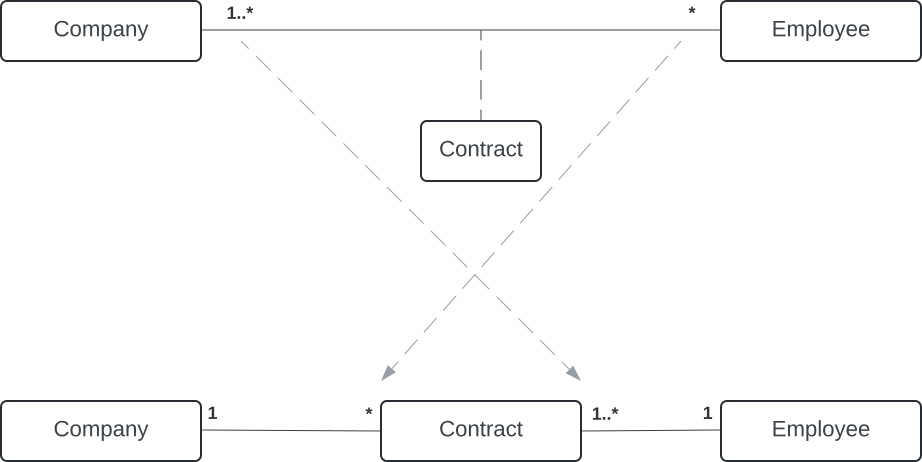
\includegraphics[scale=0.4]{part three/Klassendiagramme - Erweiterte Konzepte und Paketdiagramme/img/assoziationsklasse}
    \caption{Darstellung einer Assoziation mit Hilfe einer Assoziationsklasse (oben) sowie Transformation in gewöhnliche Assoziationen (unten). (Quelle: in Anlehnung an \cite[279, Abb. 4.4-11]{Oes05})}
    \label{fig:assoziationsklasse-cc}
\end{figure}

\clearpage


\section{Sequenzdiagramme}

\begin{tcolorbox}[title=Sequenzdiagramme]
    \textbf{Sequenzdiagramme} stellen Verhalten auf der Ebene einer Interaktion dar.\\
    In der Phase des Klassendesigns werden die Teilnehmer der Interaktionen bestimmt, weshalb Sequenzdiagramme oft in dieser Phase genutzt werden.\\
    In der \textbf{Analysephase} können Sequenzdiagramme eingesetzt werden, um die Kommunikation der bis dahin ausgemachten \textbf{Geschäftsobjekte} zu modellieren, oder um \textbf{Anwendungsfälle} weiter zu spezifizieren.
\end{tcolorbox}
\clearpage

\section{Aggregation}

\begin{tcolorbox}[title=Aggregation]
    Eine \textbf{Aggregation} ist in ihrer \semantischen Aussage unscharf (vgl.~\cite[40]{Buh09}).\\
    Sie beschreibt eine \textit{Ganzes}-\textit{Teile}-Beziehung, aber die \textit{Teile} können zu mehreren verschiedenen \textit{Ganzen} gehören.\\
    Außerdem kann ein Teil dem \textit{Ganzen} jederzeit wieder entnommen werden und das \textit{Ganze} ist nicht verantwortlich für das Erstellen der \textit{Teile}, weshalb Implementierungen beim Hinzufügen von Teilen oft schon fertige Objekte erwarten, die jeweils eines der \textit{Teile} repräsentieren.\\
    Aggregationsbeziehungen werden durch eine nicht-gefüllte Raute an der Seite der Klasse, die das Ganze repräsentiert, dargestellt.
\end{tcolorbox}
\clearpage

\section{Komposition}

\begin{tcolorbox}[title=Komposition]
    Bei einer \textbf{Komposition} handelt es sich um eine \textit{Ganzes}-\textit{Teile}-Beziehung, bei der das \textit{Ganze} verantwortlich für die Erstellung und Beseitigung der \textit{Teile} ist.
    Außerdem sind die \textit{Teile} an die \textbf{Existenz} des \textit{Ganzen} gebunden.\\
    \textit{Teile} gehören immer zu \textit{genau einem} \textit{Ganzen}.\\
    Eine Komposition wird dargestellt durch eine gefüllte Raute an der Klassenbox, die das \textit{Ganze} repräsentiert.
\end{tcolorbox}
\clearpage

\section{Paketdiagramm}

\begin{tcolorbox}[title=Komposition]
    \textbf{Paketdiagramme} zeigen Pakete und ihre Abhängigkeiten und werden in frühen Designphasen genutzt, um Strukturen (großer Systeme) aufzuzeigen.\\

    \noindent
    Elemente sollten so in Paketen gruppiert werden, dass ihr \textbf{funktionaler Zusammenhalt} (\textit{Kohäsion}, s. Abschnitt~\ref{subsec:hohe-kohasion}) klar wird.\\
    Hierdurch kann vermieden werden, dass Änderungen einer Klasse eines Paketes auch Änderungen außerhalb des Paketes erfordern.\\
    Außerdem erhöht sich die Wahrscheinlichkeit, dass einzelne Pakete als solche in anderen Projekten wiederverwendet werden können.\\

    \noindent
    In Paketdiagrammen können Beziehungen über folgende Schlüsselwörter deutlich gemacht werden:

    \begin{itemize}
        \item \guillemotleft import\guillemotright
        \item[] $\rightarrow$ \textbf{public-Import} zwischen Quell- und Zielpaket; Quellpaket kann die öffentlichen Elemente des Zielpaketes unter Verwendung des unqualifizierten und des qualifizierten Namens verwenden; die importierten Elemente sind auch für Pakete sichtbar, die das Quellpaket importieren
        \item \guillemotleft access\guillemotright
        \item[] $\rightarrow$ \textbf{privater Import} zwischen Quell- und Zielpaket; Zugriff auf Elemente des importierten Paketes ohne qualifizierenden Namen möglich; der Import eines Paketes in \textbf{Java} entspricht der \guillemotleft access\guillemotright-Beziehung
        \item \guillemotleft merge\guillemotright
        \item[] $\rightarrow$ Bei einem \textbf{merge} werden Elemente eines Zielpaketes in das Quellpaket
   \end{itemize}
\end{tcolorbox}
\clearpage

\section{Anwendungsfalldiagramm}

\begin{tcolorbox}[title=Anwendungsfalldiagramm]
    Die \textbf{Anwendungsfallanalyse} wird im Rahmen der \textbf{Anforderungsspezifikation} eingesetzt.\\

    \noindent
    Anwendungsfalldiagramme sind das am häufigsten eingesetzte Mittel zur Aufnahme und Darstellung von \textbf{Anforderungen}.\\
    Sie beschreiben selbst kein Verhalten und keine Abläufe, sondern zeigen nur die Zusammenhänge der an Anwendungsfällen beteiligten Modellelemente und sind somit ein Hilfsmittel zur Anforderungsermittlung und Verwaltung.\\

    \noindent
    Zu den wichtigsten Schritten einer Anwendungsfallanalyse gehören:
    \begin{enumerate}
        \item Akteure identifizieren
        \item Anwendungsfälle identifizieren
        \item Beschreiben der Akteure und Anwendungsfälle
        \item Identifizieren von \textit{Schlüsselobjekten}, die das System verwaltet
        \item Identifizieren der wichtigsten Anwendungsfälle (Priorisierung)
        \item detailliertere Beschreibung der Anwendungsfälle
        \item Strukturierung des Anwendungsfalldiagramms
    \end{enumerate}

    \noindent
    Anwendungsfälle beschreiben das \textbf{Szenario} der Nutzung, und nicht Features des Systems.
\end{tcolorbox}

\clearpage

\input{chapters/Anhang/CheatSheets/SE3/Aktivitätsdiagramm}
\clearpage

\section{Zustandsautomat}

\begin{tcolorbox}[title=Zustandsautomat]
    Mit \textbf{Zustandsautomaten} kann das \textit{Verhalten} von Systemen modelliert werden, wobei die \textit{Reaktionen} des Systems im Mittelpunkt stehen, und nicht die \textit{Aktionen}, wie bspw. bei den \textbf{Aktivitätsdiagrammen}.\\

    \noindent
        Ein \textbf{Zustandsautomat} kann den \textit{Lebensweg} eines Objektes modellieren, weshalb Zustandsautomaten oft im \textbf{Entwurf} als Ergänzung zu den \textbf{Klassendiagrammen} eingesetzt werden.
\end{tcolorbox}

\begin{figure}
    \centering
    \includegraphics[scale=0.4]{part three/Zustandsautomaten/img/statechartdiagramnotation}
    \caption{Elemente eines einfachen Zustandsautomaten. Eine Transitionen wird durch ein \textbf{Ereignis} ausgelöst, das ein \textit{Signal}, ein \textit{Operationsaufruf} oder auch eine bestimmte \textit{Attributänderung} sein kann. (Quelle: in Anlehnung an \cite[90, Abb. 2.11-6]{Bal05})}
    \label{fig:statechartdiagramnotation-cc}
\end{figure}

\begin{minted}[fontsize=\small]{java}
// Beispiel für eine Implementierung eines
// Parkscheinautomaten als Zustandsautomat in Java
class Parkscheinautomat {

  // zustände
  private final int BEREIT = 0;
  private final int ZAHLUNG = 1;
  private final int ABBRUCH = 2;
  private final int BELEG   = 3;

  // Zustand; wird initial beim Starten
  // des Automaten gesetzt
  private int zustand;

  // Methoden lösen Aktionen beim Eintritt
  // in die jeweiligen Zustände aus
  private int zahlung() {
    // verarbeiten
    // danach neuen Zustand zurückliefern...
    ...
    return BEREIT;
  }

   ...

  private void bereit() {
    while (true) {
      // eingabe überprüfen und
      // ggf. Zustandswechsel auslösen:
      // Zustand als Attribut setzen
      ...
    }
  }

  public void start() {
    zustand = BEREIT;

    while(true) {
      switch (zustand) {
        case BEREIT:
          zustand = bereit();
        // ... weiteres Verhalten
        ...
      }
    }
  }
}
\end{minted}
\clearpage
	

\section{Inhalt SE3}

\section*{1. Übersicht UML}

\subsection*{Lernziele}
\begin{itemize}
    \item einen Einblick in den Sprachaufbau der UML 2.0 gewinnen
    \item einen Überblick über die Diagramme der UML 2.0 und deren Zweck haben
\end{itemize}

\subsection*{Zusammenfassung}
\begin{itemize}
    \item Die \textbf{UML} ist eine weit verbreitete Modellierungssprache zur Modellierung objektorientierter Softwaresysteme.
    \item Die UML 2.0 Spezifikation besteht aus vier Teilen:
    \begin{enumerate}
        \item \textbf{Superstructure}: Diagrammtypen
        \item \textbf{Infrastructure}: Modellierungskonzepte
        \item \textbf{OCL}: formale Sprache zur Formulierung von Einschränkungen
        \item \textbf{Diagram Interchange}: Austauschformate
    \end{enumerate}
    \item Die UML kann im \textbf{Sketching} oder \textbf{Blueprint Modus} eingesetzt werden, oder als Grundlage für \textbf{automatische Codegenerierung}
    \item Die UML ist an keinen speziellen Entwicklungsprozess gebunden
\end{itemize}

\section*{2. Klassendiagramme}

\subsection*{Lernziele}
\begin{itemize}
    \item wissen, wie Klassendiagramme im Entwicklungsprozess eingesetzt werden
    \item Klassendiagramme für Analyse- und Designentscheidungen einsetzen können
    \item die wichtigsten Modellierungskonzepte kennen
    \item sinnvolle Klassendiagramme erstellen und Java-Implementierungen ableiten können
    \item Klassendiagramme aus Java Quellcode erzeugen können
\end{itemize}

\subsection*{Zusammenfassung}

\begin{itemize}
    \item \textbf{Klassendiagramme} dienen zur \textbf{strukturellen Darstellung} von Softwaresystemen
    \item hierbei werden Klassen und \textbf{Beziehungen} zwischen Klassen dargestellt
    \item Properties können durch die \textbf{Attribut}- oder \textbf{Assoziationsnotation} modelliert werden
    \item Operationen werden als separate Zeile in ihrem Compartment dargestellt
    \item im Klassendiagramm können auch \textbf{Generalisierungsbeziehungen} modelliert werden
    \item \textbf{Abhängigkeitsbeziehungen} drücken ein Verhältnis zwischen \textbf{Client} und \textbf{Supplier} aus
\end{itemize}

\section*{3. Objektorientierter Entwurf}

\subsection*{Lernziele}
\begin{itemize}
    \item das Wesen einer Interaktion kennen
    \item wissen, wie Sequenzdiagramme im Entwicklungsprozess eingesetzt werden
    \item Sequenzdiagramme für Analyse- und Designentscheidungen sowie zur Darstellung von Kontrollflüssen einsetzen können
    \item die wichtigsten Modellierungskonzepte kennen
    \item sinnvolle Sequenzdiagramme erstellen und Java-Implementierungen ableiten können
    \item Sequenzdiagramme aus Java Quellcode erzeugen können
\end{itemize}

\subsection*{Zusammenfassung}

\begin{itemize}
    \item Sequenzdiagramme sind \textbf{Verhaltensdiagramme}
    und können im gesamten Entwicklungszyklus zur Modellierung von Interaktionen angewendet werden
    \item Interaktionen bestehen im Wesentlichen aus dem Nachrichtenaustausch zwischen verschiedenen Kommunikationspartnern
    \item in den meisten Fällen wird die Kommunikation von Objekten von Klassen modelliert, aber es können auch Teilnehmer auf anderen Ebenen modelliert werden
    \item gewöhnlich gibt ein Sequenzdiagramm einen \textbf{Anwendungsfall} (\textit{Szenario}) wieder
    \item sie dienen nicht dazu, um Zustandsänderungen darzustellen (hierfür werden Zustandsdiagramme verwendet)
    \item Sequenzdiagramme sind \textit{nicht} gut geeignet für die Darstellung von
    \begin{itemize}
        \item nebenläufigem Verhalten (\textit{asynchrone} Nachrichten, \textit{kombiniertes Fragment})
        \item Schleifen und alternativem Verhalten (\textit{kombinierte Fragmente})
        \item[] $\rightarrow$  für beide Fälle sind \textbf{Aktivitätsdiagramme} besser geeignet
    \end{itemize}
\end{itemize}

\section*{4. Klassendiagramme - Erweiterte Konzepte und Paketdiagramme}

\subsection*{Lernziele}
\begin{itemize}
    \item erweiterte Modellierungskonzepte in Klassendiagrammen für den Detailentwurf von Systemen kennen
    \item die Konsequenzen dieser Konzepte in der Implementierung kennen
    \item wissen, wie Paketdiagramme im Entwicklungsprozess eingesetzt werden
    \item die Modellierungskonzepte in Paketdiagrammen kennen
    \item anhand von Paketdiagrammen Software-Architekturen gestalten und bewerten können
\end{itemize}

\subsection*{Zusammenfassung}

\begin{itemize}
    \item Die vorgestellten erweiterten Konzepte werden vor allem im \textbf{Feinentwurf} von Klassenstrukturen eingesetzt.
    \item Generell gilt, dass die Spezifikationen von Objekten und Properties nur so detailliert ausgeführt werden sollen, wie nötig: Sind Details für das Verständnis unnötig, sollte darauf verzichtet werden.
    \item \textbf{Generalisierungsbeziehungen} sollten grundsätzlich modelliert werden.
    \item Ist eine \textbf{Komposition} statt einer Generalisierung für den Sachverhalt möglich, sollte diese verwendet werden: ``Favor object composition over inheritance.`` (\cite[19 f.]{GHJV94})
    \item \textbf{Kompositionsbeziehungen} geben eindeutige Impulse für eine Implementierung, \textbf{Aggregationsbeziehungen} sind in ihrer semantischen Aussage nicht sehr eindeutig
    \item \textbf{Assoziationsklassen} sind in ihrer frühen Designphase empfehlenswert, die Realisierung (mit {bspw.} Java) erfordert aber eine Transformation in eine volle Klasse, wobei die Multiplizitäten angepasst werden müssen
    \item Elemente können in \textbf{Paketen} zusamengefasst und unter einem gemeinsamen Namensraum gruppiert werden
\end{itemize}

\section*{4. Anwendungsfalldiagramm (Use-Case-Diagramm)}

\subsection*{Lernziele}
\begin{itemize}
    \item wissen, wie die Anwendungsfallanalyse im Rahmen der Anforderungsspezifikation eingesetzt wird
    \item Prozessschritte der Anwendungsfallanalyse beherrschen
    \item die wichtigsten Modellierungskonzepte in Anwendungsfalldiagrammen kennen
    \item den Aufbau einer Anwendungsfallbeschreibung kennen
\end{itemize}

\subsection*{Zusammenfassung}

\begin{itemize}
    \item \textbf{Anwendungsfalldiagramme} besitzen eine einfache Notation, um \textbf{Akteure} und \textbf{Anwendungsfälle} eines \textbf{Systems} grafisch darzustellen
    \item auf Basis eines Anwendungsfalldiagramms lässt sich ermitteln, ob die Anwendungsfälle gewünschtes Verhalten realisieren bzw. Beziehungen zu einem oder mehreren Akteuren haben
    \item Anwendungsfälle und Akteure \textit{müssen} zusätzlich textlich beschrieben werden
\end{itemize}

\section*{5. Aktivitätsdiagramme}

\subsection*{Lernziele}
\begin{itemize}
    \item wissen, wie Aktivitätsdiagramme im Rahmen der Verhaltensanalyse in verschiedenen Prozessphasen eingesetzt werden können
    \item die wichtigsten Modellierungskonzepte in Aktivitätsdiagrammen kennen
    \item Aktivitätsdiagramme interpretieren, erstellen und implementieren können
\end{itemize}

\subsection*{Zusammenfassung}

\begin{itemize}
    \item \textbf{Aktivitätsdiagramme} gehören zu den \textbf{Verhaltensdiagrammen} und können im \textit{gesamten} \textbf{Entwicklungsprozess} eingesetzt werden
    \item durch ein Aktivitätsdiagramm kann gezeigt werden, wie \textbf{Verhalten} realisiert wird
    \item es können mehrere \textbf{Aktivitäten} dargestellt werden
    \item \textbf{Aktivitätskanten} und \textbf{Aktivitätsknoten} werden zur Beschreibung von Verhalten verwendet
\end{itemize}

\section*{5. Zustandsautomaten}

\subsection*{Lernziele}
\begin{itemize}
    \item wissen, wie Zustandsdiagramme im Rahmen der Verhaltensanalyse einzelner Objekte eingesetzt werden können
    \item die wichtigsten Modellierungskonzepte in Zustandsdiagrammen kennen
    \item Zustandsdiagramme interpretieren, erstellen und implementieren können
\end{itemize}

\subsection*{Zusammenfassung}

\begin{itemize}
    \item Das \textbf{Zustandsdiagramm} gehört wie das \textbf{Aktivitätsdiagramm} zu den \textbf{Verhaltensdiagrammen}.
    \item Ein Zustandsdiagramm zeigt den \textbf{Lebensweg} eines \textbf{Objektes}.
    \item \textbf{Attributwerte} bestimmen den Zustand eines Objektes.
    \item \textbf{Transitionen} zwischen Zuständen werden durch \textbf{Guards} und \textbf{Events} gesteuert.
    \item Während der Transitionen können \textbf{Effekte} (\textit{Aktivitäten}) realisiert werden.
    \item Die Modellierung \textbf{zusammengesetzter Zustände} ist ebenfalls möglich.
    \item Für die Darstellung \textbf{paralleler} oder  \textbf{konkurrierender} Abläufe können \textbf{Regionen} modelliert werden.
\end{itemize}
\clearpage


\section{UML Modellierung}

\begin{tcolorbox}[title=UML Modellierung]
    \textbf{Modelle} haben die Aufgabe, den Bezug zum Original (Programm, Softwaresystem) herzustellen, sowie zu der \textit{Anwendungsumgebung}.\\
    Ein \textbf{Modell} enthält alle \textbf{Modellelemente}, die zur Beschreibung eines Softwaresystems nötig sind.\\

    \noindent
    Ein \textbf{Modellelement} wird als Element in einem UML Modell von einem Benutzer erstellt und auf verschiedenen \textbf{Diagrammen} (Struktur-/Verhaltensdiagrammen) platziert, und wird durch die \textbf{UML Modellierungskonzepte} als Metaklasse des \textbf{Metamodells} der UML beschrieben: \textbf{Modellelemente} werden aus Modellierungskonzepten instanziiert.\\

    \noindent
       Das \textbf{UML Metamodell} regelt, in welchem Zusammenhang \textbf{UML Modellierungskonzepte} in Modellen auftreten dürfen, und welche Eigenschaften und Beziehungen zu anderen Sprachelementen zulässig sind.\\

       \noindent
       Die im \textbf{Metamodell} verwendeten Erklärungen basieren auf einer abstrakten Syntax, für deren Beschreibung eine Untermenge (\textit{Klassendiagramme}) der UML verwendet wird.\\
        Die \textbf{Semantik} der Modellierungskonzepte wird textlich beschrieben, zur Formalisierung von Regeln für die syntaktische Korrektheit wird die \textbf{OCL} (\textit{Object Constraint Language}) verwendet.
\end{tcolorbox}

\begin{figure}
    \centering
    \includegraphics[scale=0.4]{part three/Einführung/img/metamodel}
    \caption{Beispiel für die verschiedenen Schichten der Metamodell Hierarchie.
        In der original Abbildung sind die Pfeilspitzen offen. (Quelle: in Anlehnung an S. 20, Figure 7.8, \url{https://www.omg.org/spec/UML/2.4.1/Infrastructure/PDF}, abgerufen 01.05.2024}
    \label{fig:metamodel-cc}
\end{figure}

\clearpage


\section{Strukturdiagramme}

\begin{tcolorbox}[title=Strukturdiagramme]
    In den \textbf{Strukturdiagrammen} werden \textbf{statische Strukturaspekte} eines Systems betrachtet.
    Für eine Systemmodellierung können alle dieser 6 Diagramme verwendet werden.

    \begin{itemize}
        \item \textbf{Klassendiagramm}: Das \textbf{Klassendiagramm} wird verwendet, um ein objektorientiertes System zu beschreiben.
        \item \textbf{Paketdiagramm}: Ein \textbf{Paketdiagramm} zeigt die Pakete eines Systems und deren Beziehungen.
        \item \textbf{Komponentendiagramm}: Stellt Komponenten oder auch \textit{Subsysteme} mit definierten Interfaces dar, um bspw. \textbf{Architekturdesign} darzustellen.
        \item \textbf{Verteilungsdiagramm}: Beschreibt eine Menge von Knoten, die die \textit{Ausführungsarchitektur} eines Systems definieren können, wobei Knoten i.d.R. \textit{Geräte} oder \textit{Softwareablaufumgebungen repräsentieren}.
        \item \textbf{Kompositionsstrukturdiagramm}: Stellt die \textbf{Komposition} von \textit{Systemstrukturen} (Klassen, Komponenten, Gesamtsystem) in einem bestimmten \textit{Kontext} mit einem bestimmten \textit{Ziel} dar (vgl. \cite[9]{Buh09}).
        \item \textbf{Objektdiagramm}: Momentaufnahme eines Systems zu genau einem \textit{Zeitpukt} während der Ausführung
    \end{itemize}

\end{tcolorbox}
\clearpage

\section{Verhaltensdiagramme}

\begin{tcolorbox}[title=Verhaltensdiagramme]
    \textbf{Verhaltensdiagramme} stellen \textit{Dynamik}, \textit{interne Abläufe} und das \textit{Zusammenspiel} der Systemteile dar, um eine Spezifikation zu vervollständigen.

    \begin{itemize}
        \item \textbf{Anwendungsfalldiagramm}: Dienen zur \textit{Spezifizierung} und \textit{Formalisierung} von \textit{Systemanforderungen}, unter Berücksichtigung von \textbf{Akteuren}, \textbf{Systemen} und \textbf{Anwendungsfällen}
        \item \textbf{Zustandsdiagramm}: Auch \textbf{Zustandsautomaten}; zeigen für ein einzelnes Objekt Zustandsänderungen während der Lebenszeit
        \item \textbf{Aktivitätsdiagramme}: Werden zur Modellierung von \textit{Kontroll}- oder \textit{Objektflüssen} oder zur Darstellung von \textit{Programmlogik} genutzt.
        \item \textbf{Interaktionsdiagramme}: Stellen das Zusammenspiel mehrerer Kommunikationspartner dar.
        Es gibt unterschiedliche Typen von Interaktionsdiagrammen, die Interaktionen auf verschiedenen \textit{Abstraktionsebenen} modellieren:
        \begin{itemize}
            \item \textbf{Sequenzdiagramm}: Zeigt den Verlauf einer Interaktion in zwei Dimensionen, \textit{Kommunikationspartner} und die Nachrichten in ihrer \textit{zeitlichen Abfolge}
            \item \textbf{Kommunikationsdiagramm}: hebt die Kommunikationsbeziehungen zwischen den Partnern hervor
            \item \textbf{Timing Diagramm}: hebt die zeitlichen Aspekte einer Interaktion hervor
            \item \textbf{Interaktionsüberblickdiagramm}: Spezialfall des \textbf{Aktivitätsdiagramms} - statt Aktionen und Aktivitäten können das \textbf{Sequenz}-, \textbf{Kommunikations}- und das \textbf{Timing}-Diagramm als Knoten verwendet werden.
        \end{itemize}
        Alle verwenden dieselben Grundelemente: \textit{Lebenslinien} der Akteure und Nachrichten, die zwischen diesen ausgetauscht werden.
    \end{itemize}
\end{tcolorbox}

\clearpage


\section{Klassendiagramm}

\begin{tcolorbox}[title=Klassendiagramm]
    Das \textbf{Klassendiagramm} beschreibt die Klassen eines Systems und die statischen Beziehungen zwischen ihnen.\\
    Sie werden in Form von Domainklassen bei der \textbf{Analyse} und als detaillierte Entwürfe von Systemklassen als \textit{Blueprint} im \textbf{gesamten Entwicklungsprozess} eingesetzt.

\end{tcolorbox}
\clearpage


\section{Assoziationsklasse (Attributierte Assoziation)}

\begin{tcolorbox}[title=Assoziationsklasse (Attributierte Assoziation)]
Eine \textbf{Assoziationsklasse} erlaubt das Hinzufügen von Operationen und Attributen zu einer Assoziation (\cite[43]{Buh09}).\\
Assoziationsklassen werden in der \textbf{Analyse} in Modellen verwendet und in dem \textbf{Entwurf} in eigenständige Klassen transformiert.\\

\noindent
Assoziationsklassen werden in der \textbf{Analyse} in Modellen verwendet und in dem \textbf{Entwurf} in eigenständige Klassen transformiert.

\blockquote[{\cite[277]{Oes05}}]{
    Eine attributierte Assoziation ist immer dann nahe liegend, wenn Attribute oder Operationen gefunden werden, die weder der einen noch der anderen Klasse zugeordnet werden können, weil sie nämlich Eigenschaften der Beziehung selbst sind.
}.\\

Bei einer attributierten Assoziation dürfen zwei beteiligte Objekte maximal nur eine Beziehung zueinander haben (vgl.~\cite[277]{Oes05})\footnote{
    \textit{Ostereich} führt dies ebenda auf Seite 278 weiter aus, in dem er beschreibt, wie eine attributierte Assoziation für ein \textit{Beschäftigtenverhältnis} zwischen \textit{Mitarbeiter} und \textit{Unternehmen} modelliert wird. Dabei wird davon ausgegangen, dass ein \textit{Mitarbeiter} nur über \textit{ein} Arbeitsverhältnis mit einem \textit{Unternehmen} in Beziehung stehen kann. Bestehen mehrere Arbeitsverhältnisse (\textit{Mitarbeiter} hat zu unterschiedlichen Zeitpunkten für das \textit{Unternehmen} gearbeitet), kann die attributierte Assoziation nicht verwendet werden.\\

\noindent
Wird eine attributierte Assoziation in eine gewöhnliche Assoziation transformiert, muss darauf geachtet werden, die Multiplizitäten richtig zu setzen (s. Abbildung~\ref{fig:assoziationsklasse}).
\end{tcolorbox}

\begin{figure}
    \centering
    \includegraphics[scale=0.4]{part three/Klassendiagramme - Erweiterte Konzepte und Paketdiagramme/img/assoziationsklasse}
    \caption{Darstellung einer Assoziation mit Hilfe einer Assoziationsklasse (oben) sowie Transformation in gewöhnliche Assoziationen (unten). (Quelle: in Anlehnung an \cite[279, Abb. 4.4-11]{Oes05})}
    \label{fig:assoziationsklasse-cc}
\end{figure}

\clearpage


\section{Sequenzdiagramme}

\begin{tcolorbox}[title=Sequenzdiagramme]
    \textbf{Sequenzdiagramme} stellen Verhalten auf der Ebene einer Interaktion dar.\\
    In der Phase des Klassendesigns werden die Teilnehmer der Interaktionen bestimmt, weshalb Sequenzdiagramme oft in dieser Phase genutzt werden.\\
    In der \textbf{Analysephase} können Sequenzdiagramme eingesetzt werden, um die Kommunikation der bis dahin ausgemachten \textbf{Geschäftsobjekte} zu modellieren, oder um \textbf{Anwendungsfälle} weiter zu spezifizieren.
\end{tcolorbox}
\clearpage

\section{Aggregation}

\begin{tcolorbox}[title=Aggregation]
    Eine \textbf{Aggregation} ist in ihrer \semantischen Aussage unscharf (vgl.~\cite[40]{Buh09}).\\
    Sie beschreibt eine \textit{Ganzes}-\textit{Teile}-Beziehung, aber die \textit{Teile} können zu mehreren verschiedenen \textit{Ganzen} gehören.\\
    Außerdem kann ein Teil dem \textit{Ganzen} jederzeit wieder entnommen werden und das \textit{Ganze} ist nicht verantwortlich für das Erstellen der \textit{Teile}, weshalb Implementierungen beim Hinzufügen von Teilen oft schon fertige Objekte erwarten, die jeweils eines der \textit{Teile} repräsentieren.\\
    Aggregationsbeziehungen werden durch eine nicht-gefüllte Raute an der Seite der Klasse, die das Ganze repräsentiert, dargestellt.
\end{tcolorbox}
\clearpage

\section{Komposition}

\begin{tcolorbox}[title=Komposition]
    Bei einer \textbf{Komposition} handelt es sich um eine \textit{Ganzes}-\textit{Teile}-Beziehung, bei der das \textit{Ganze} verantwortlich für die Erstellung und Beseitigung der \textit{Teile} ist.
    Außerdem sind die \textit{Teile} an die \textbf{Existenz} des \textit{Ganzen} gebunden.\\
    \textit{Teile} gehören immer zu \textit{genau einem} \textit{Ganzen}.\\
    Eine Komposition wird dargestellt durch eine gefüllte Raute an der Klassenbox, die das \textit{Ganze} repräsentiert.
\end{tcolorbox}
\clearpage

\section{Paketdiagramm}

\begin{tcolorbox}[title=Komposition]
    \textbf{Paketdiagramme} zeigen Pakete und ihre Abhängigkeiten und werden in frühen Designphasen genutzt, um Strukturen (großer Systeme) aufzuzeigen.\\

    \noindent
    Elemente sollten so in Paketen gruppiert werden, dass ihr \textbf{funktionaler Zusammenhalt} (\textit{Kohäsion}, s. Abschnitt~\ref{subsec:hohe-kohasion}) klar wird.\\
    Hierdurch kann vermieden werden, dass Änderungen einer Klasse eines Paketes auch Änderungen außerhalb des Paketes erfordern.\\
    Außerdem erhöht sich die Wahrscheinlichkeit, dass einzelne Pakete als solche in anderen Projekten wiederverwendet werden können.\\

    \noindent
    In Paketdiagrammen können Beziehungen über folgende Schlüsselwörter deutlich gemacht werden:

    \begin{itemize}
        \item \guillemotleft import\guillemotright
        \item[] $\rightarrow$ \textbf{public-Import} zwischen Quell- und Zielpaket; Quellpaket kann die öffentlichen Elemente des Zielpaketes unter Verwendung des unqualifizierten und des qualifizierten Namens verwenden; die importierten Elemente sind auch für Pakete sichtbar, die das Quellpaket importieren
        \item \guillemotleft access\guillemotright
        \item[] $\rightarrow$ \textbf{privater Import} zwischen Quell- und Zielpaket; Zugriff auf Elemente des importierten Paketes ohne qualifizierenden Namen möglich; der Import eines Paketes in \textbf{Java} entspricht der \guillemotleft access\guillemotright-Beziehung
        \item \guillemotleft merge\guillemotright
        \item[] $\rightarrow$ Bei einem \textbf{merge} werden Elemente eines Zielpaketes in das Quellpaket
   \end{itemize}
\end{tcolorbox}
\clearpage

\section{Anwendungsfalldiagramm}

\begin{tcolorbox}[title=Anwendungsfalldiagramm]
    Die \textbf{Anwendungsfallanalyse} wird im Rahmen der \textbf{Anforderungsspezifikation} eingesetzt.\\

    \noindent
    Anwendungsfalldiagramme sind das am häufigsten eingesetzte Mittel zur Aufnahme und Darstellung von \textbf{Anforderungen}.\\
    Sie beschreiben selbst kein Verhalten und keine Abläufe, sondern zeigen nur die Zusammenhänge der an Anwendungsfällen beteiligten Modellelemente und sind somit ein Hilfsmittel zur Anforderungsermittlung und Verwaltung.\\

    \noindent
    Zu den wichtigsten Schritten einer Anwendungsfallanalyse gehören:
    \begin{enumerate}
        \item Akteure identifizieren
        \item Anwendungsfälle identifizieren
        \item Beschreiben der Akteure und Anwendungsfälle
        \item Identifizieren von \textit{Schlüsselobjekten}, die das System verwaltet
        \item Identifizieren der wichtigsten Anwendungsfälle (Priorisierung)
        \item detailliertere Beschreibung der Anwendungsfälle
        \item Strukturierung des Anwendungsfalldiagramms
    \end{enumerate}

    \noindent
    Anwendungsfälle beschreiben das \textbf{Szenario} der Nutzung, und nicht Features des Systems.
\end{tcolorbox}

\clearpage

\input{chapters/Anhang/CheatSheets/SE3/Aktivitätsdiagramm}
\clearpage

\section{Zustandsautomat}

\begin{tcolorbox}[title=Zustandsautomat]
    Mit \textbf{Zustandsautomaten} kann das \textit{Verhalten} von Systemen modelliert werden, wobei die \textit{Reaktionen} des Systems im Mittelpunkt stehen, und nicht die \textit{Aktionen}, wie bspw. bei den \textbf{Aktivitätsdiagrammen}.\\

    \noindent
        Ein \textbf{Zustandsautomat} kann den \textit{Lebensweg} eines Objektes modellieren, weshalb Zustandsautomaten oft im \textbf{Entwurf} als Ergänzung zu den \textbf{Klassendiagrammen} eingesetzt werden.
\end{tcolorbox}

\begin{figure}
    \centering
    \includegraphics[scale=0.4]{part three/Zustandsautomaten/img/statechartdiagramnotation}
    \caption{Elemente eines einfachen Zustandsautomaten. Eine Transitionen wird durch ein \textbf{Ereignis} ausgelöst, das ein \textit{Signal}, ein \textit{Operationsaufruf} oder auch eine bestimmte \textit{Attributänderung} sein kann. (Quelle: in Anlehnung an \cite[90, Abb. 2.11-6]{Bal05})}
    \label{fig:statechartdiagramnotation-cc}
\end{figure}

\begin{minted}[fontsize=\small]{java}
// Beispiel für eine Implementierung eines
// Parkscheinautomaten als Zustandsautomat in Java
class Parkscheinautomat {

  // zustände
  private final int BEREIT = 0;
  private final int ZAHLUNG = 1;
  private final int ABBRUCH = 2;
  private final int BELEG   = 3;

  // Zustand; wird initial beim Starten
  // des Automaten gesetzt
  private int zustand;

  // Methoden lösen Aktionen beim Eintritt
  // in die jeweiligen Zustände aus
  private int zahlung() {
    // verarbeiten
    // danach neuen Zustand zurückliefern...
    ...
    return BEREIT;
  }

   ...

  private void bereit() {
    while (true) {
      // eingabe überprüfen und
      // ggf. Zustandswechsel auslösen:
      // Zustand als Attribut setzen
      ...
    }
  }

  public void start() {
    zustand = BEREIT;

    while(true) {
      switch (zustand) {
        case BEREIT:
          zustand = bereit();
        // ... weiteres Verhalten
        ...
      }
    }
  }
}
\end{minted}
\clearpage
	

\section{Inhalt SE3}

\section*{1. Übersicht UML}

\subsection*{Lernziele}
\begin{itemize}
    \item einen Einblick in den Sprachaufbau der UML 2.0 gewinnen
    \item einen Überblick über die Diagramme der UML 2.0 und deren Zweck haben
\end{itemize}

\subsection*{Zusammenfassung}
\begin{itemize}
    \item Die \textbf{UML} ist eine weit verbreitete Modellierungssprache zur Modellierung objektorientierter Softwaresysteme.
    \item Die UML 2.0 Spezifikation besteht aus vier Teilen:
    \begin{enumerate}
        \item \textbf{Superstructure}: Diagrammtypen
        \item \textbf{Infrastructure}: Modellierungskonzepte
        \item \textbf{OCL}: formale Sprache zur Formulierung von Einschränkungen
        \item \textbf{Diagram Interchange}: Austauschformate
    \end{enumerate}
    \item Die UML kann im \textbf{Sketching} oder \textbf{Blueprint Modus} eingesetzt werden, oder als Grundlage für \textbf{automatische Codegenerierung}
    \item Die UML ist an keinen speziellen Entwicklungsprozess gebunden
\end{itemize}

\section*{2. Klassendiagramme}

\subsection*{Lernziele}
\begin{itemize}
    \item wissen, wie Klassendiagramme im Entwicklungsprozess eingesetzt werden
    \item Klassendiagramme für Analyse- und Designentscheidungen einsetzen können
    \item die wichtigsten Modellierungskonzepte kennen
    \item sinnvolle Klassendiagramme erstellen und Java-Implementierungen ableiten können
    \item Klassendiagramme aus Java Quellcode erzeugen können
\end{itemize}

\subsection*{Zusammenfassung}

\begin{itemize}
    \item \textbf{Klassendiagramme} dienen zur \textbf{strukturellen Darstellung} von Softwaresystemen
    \item hierbei werden Klassen und \textbf{Beziehungen} zwischen Klassen dargestellt
    \item Properties können durch die \textbf{Attribut}- oder \textbf{Assoziationsnotation} modelliert werden
    \item Operationen werden als separate Zeile in ihrem Compartment dargestellt
    \item im Klassendiagramm können auch \textbf{Generalisierungsbeziehungen} modelliert werden
    \item \textbf{Abhängigkeitsbeziehungen} drücken ein Verhältnis zwischen \textbf{Client} und \textbf{Supplier} aus
\end{itemize}

\section*{3. Objektorientierter Entwurf}

\subsection*{Lernziele}
\begin{itemize}
    \item das Wesen einer Interaktion kennen
    \item wissen, wie Sequenzdiagramme im Entwicklungsprozess eingesetzt werden
    \item Sequenzdiagramme für Analyse- und Designentscheidungen sowie zur Darstellung von Kontrollflüssen einsetzen können
    \item die wichtigsten Modellierungskonzepte kennen
    \item sinnvolle Sequenzdiagramme erstellen und Java-Implementierungen ableiten können
    \item Sequenzdiagramme aus Java Quellcode erzeugen können
\end{itemize}

\subsection*{Zusammenfassung}

\begin{itemize}
    \item Sequenzdiagramme sind \textbf{Verhaltensdiagramme}
    und können im gesamten Entwicklungszyklus zur Modellierung von Interaktionen angewendet werden
    \item Interaktionen bestehen im Wesentlichen aus dem Nachrichtenaustausch zwischen verschiedenen Kommunikationspartnern
    \item in den meisten Fällen wird die Kommunikation von Objekten von Klassen modelliert, aber es können auch Teilnehmer auf anderen Ebenen modelliert werden
    \item gewöhnlich gibt ein Sequenzdiagramm einen \textbf{Anwendungsfall} (\textit{Szenario}) wieder
    \item sie dienen nicht dazu, um Zustandsänderungen darzustellen (hierfür werden Zustandsdiagramme verwendet)
    \item Sequenzdiagramme sind \textit{nicht} gut geeignet für die Darstellung von
    \begin{itemize}
        \item nebenläufigem Verhalten (\textit{asynchrone} Nachrichten, \textit{kombiniertes Fragment})
        \item Schleifen und alternativem Verhalten (\textit{kombinierte Fragmente})
        \item[] $\rightarrow$  für beide Fälle sind \textbf{Aktivitätsdiagramme} besser geeignet
    \end{itemize}
\end{itemize}

\section*{4. Klassendiagramme - Erweiterte Konzepte und Paketdiagramme}

\subsection*{Lernziele}
\begin{itemize}
    \item erweiterte Modellierungskonzepte in Klassendiagrammen für den Detailentwurf von Systemen kennen
    \item die Konsequenzen dieser Konzepte in der Implementierung kennen
    \item wissen, wie Paketdiagramme im Entwicklungsprozess eingesetzt werden
    \item die Modellierungskonzepte in Paketdiagrammen kennen
    \item anhand von Paketdiagrammen Software-Architekturen gestalten und bewerten können
\end{itemize}

\subsection*{Zusammenfassung}

\begin{itemize}
    \item Die vorgestellten erweiterten Konzepte werden vor allem im \textbf{Feinentwurf} von Klassenstrukturen eingesetzt.
    \item Generell gilt, dass die Spezifikationen von Objekten und Properties nur so detailliert ausgeführt werden sollen, wie nötig: Sind Details für das Verständnis unnötig, sollte darauf verzichtet werden.
    \item \textbf{Generalisierungsbeziehungen} sollten grundsätzlich modelliert werden.
    \item Ist eine \textbf{Komposition} statt einer Generalisierung für den Sachverhalt möglich, sollte diese verwendet werden: ``Favor object composition over inheritance.`` (\cite[19 f.]{GHJV94})
    \item \textbf{Kompositionsbeziehungen} geben eindeutige Impulse für eine Implementierung, \textbf{Aggregationsbeziehungen} sind in ihrer semantischen Aussage nicht sehr eindeutig
    \item \textbf{Assoziationsklassen} sind in ihrer frühen Designphase empfehlenswert, die Realisierung (mit {bspw.} Java) erfordert aber eine Transformation in eine volle Klasse, wobei die Multiplizitäten angepasst werden müssen
    \item Elemente können in \textbf{Paketen} zusamengefasst und unter einem gemeinsamen Namensraum gruppiert werden
\end{itemize}

\section*{4. Anwendungsfalldiagramm (Use-Case-Diagramm)}

\subsection*{Lernziele}
\begin{itemize}
    \item wissen, wie die Anwendungsfallanalyse im Rahmen der Anforderungsspezifikation eingesetzt wird
    \item Prozessschritte der Anwendungsfallanalyse beherrschen
    \item die wichtigsten Modellierungskonzepte in Anwendungsfalldiagrammen kennen
    \item den Aufbau einer Anwendungsfallbeschreibung kennen
\end{itemize}

\subsection*{Zusammenfassung}

\begin{itemize}
    \item \textbf{Anwendungsfalldiagramme} besitzen eine einfache Notation, um \textbf{Akteure} und \textbf{Anwendungsfälle} eines \textbf{Systems} grafisch darzustellen
    \item auf Basis eines Anwendungsfalldiagramms lässt sich ermitteln, ob die Anwendungsfälle gewünschtes Verhalten realisieren bzw. Beziehungen zu einem oder mehreren Akteuren haben
    \item Anwendungsfälle und Akteure \textit{müssen} zusätzlich textlich beschrieben werden
\end{itemize}

\section*{5. Aktivitätsdiagramme}

\subsection*{Lernziele}
\begin{itemize}
    \item wissen, wie Aktivitätsdiagramme im Rahmen der Verhaltensanalyse in verschiedenen Prozessphasen eingesetzt werden können
    \item die wichtigsten Modellierungskonzepte in Aktivitätsdiagrammen kennen
    \item Aktivitätsdiagramme interpretieren, erstellen und implementieren können
\end{itemize}

\subsection*{Zusammenfassung}

\begin{itemize}
    \item \textbf{Aktivitätsdiagramme} gehören zu den \textbf{Verhaltensdiagrammen} und können im \textit{gesamten} \textbf{Entwicklungsprozess} eingesetzt werden
    \item durch ein Aktivitätsdiagramm kann gezeigt werden, wie \textbf{Verhalten} realisiert wird
    \item es können mehrere \textbf{Aktivitäten} dargestellt werden
    \item \textbf{Aktivitätskanten} und \textbf{Aktivitätsknoten} werden zur Beschreibung von Verhalten verwendet
\end{itemize}

\section*{5. Zustandsautomaten}

\subsection*{Lernziele}
\begin{itemize}
    \item wissen, wie Zustandsdiagramme im Rahmen der Verhaltensanalyse einzelner Objekte eingesetzt werden können
    \item die wichtigsten Modellierungskonzepte in Zustandsdiagrammen kennen
    \item Zustandsdiagramme interpretieren, erstellen und implementieren können
\end{itemize}

\subsection*{Zusammenfassung}

\begin{itemize}
    \item Das \textbf{Zustandsdiagramm} gehört wie das \textbf{Aktivitätsdiagramm} zu den \textbf{Verhaltensdiagrammen}.
    \item Ein Zustandsdiagramm zeigt den \textbf{Lebensweg} eines \textbf{Objektes}.
    \item \textbf{Attributwerte} bestimmen den Zustand eines Objektes.
    \item \textbf{Transitionen} zwischen Zuständen werden durch \textbf{Guards} und \textbf{Events} gesteuert.
    \item Während der Transitionen können \textbf{Effekte} (\textit{Aktivitäten}) realisiert werden.
    \item Die Modellierung \textbf{zusammengesetzter Zustände} ist ebenfalls möglich.
    \item Für die Darstellung \textbf{paralleler} oder  \textbf{konkurrierender} Abläufe können \textbf{Regionen} modelliert werden.
\end{itemize}
\clearpage


\section{UML Modellierung}

\begin{tcolorbox}[title=UML Modellierung]
    \textbf{Modelle} haben die Aufgabe, den Bezug zum Original (Programm, Softwaresystem) herzustellen, sowie zu der \textit{Anwendungsumgebung}.\\
    Ein \textbf{Modell} enthält alle \textbf{Modellelemente}, die zur Beschreibung eines Softwaresystems nötig sind.\\

    \noindent
    Ein \textbf{Modellelement} wird als Element in einem UML Modell von einem Benutzer erstellt und auf verschiedenen \textbf{Diagrammen} (Struktur-/Verhaltensdiagrammen) platziert, und wird durch die \textbf{UML Modellierungskonzepte} als Metaklasse des \textbf{Metamodells} der UML beschrieben: \textbf{Modellelemente} werden aus Modellierungskonzepten instanziiert.\\

    \noindent
       Das \textbf{UML Metamodell} regelt, in welchem Zusammenhang \textbf{UML Modellierungskonzepte} in Modellen auftreten dürfen, und welche Eigenschaften und Beziehungen zu anderen Sprachelementen zulässig sind.\\

       \noindent
       Die im \textbf{Metamodell} verwendeten Erklärungen basieren auf einer abstrakten Syntax, für deren Beschreibung eine Untermenge (\textit{Klassendiagramme}) der UML verwendet wird.\\
        Die \textbf{Semantik} der Modellierungskonzepte wird textlich beschrieben, zur Formalisierung von Regeln für die syntaktische Korrektheit wird die \textbf{OCL} (\textit{Object Constraint Language}) verwendet.
\end{tcolorbox}

\begin{figure}
    \centering
    \includegraphics[scale=0.4]{part three/Einführung/img/metamodel}
    \caption{Beispiel für die verschiedenen Schichten der Metamodell Hierarchie.
        In der original Abbildung sind die Pfeilspitzen offen. (Quelle: in Anlehnung an S. 20, Figure 7.8, \url{https://www.omg.org/spec/UML/2.4.1/Infrastructure/PDF}, abgerufen 01.05.2024}
    \label{fig:metamodel-cc}
\end{figure}

\clearpage


\section{Strukturdiagramme}

\begin{tcolorbox}[title=Strukturdiagramme]
    In den \textbf{Strukturdiagrammen} werden \textbf{statische Strukturaspekte} eines Systems betrachtet.
    Für eine Systemmodellierung können alle dieser 6 Diagramme verwendet werden.

    \begin{itemize}
        \item \textbf{Klassendiagramm}: Das \textbf{Klassendiagramm} wird verwendet, um ein objektorientiertes System zu beschreiben.
        \item \textbf{Paketdiagramm}: Ein \textbf{Paketdiagramm} zeigt die Pakete eines Systems und deren Beziehungen.
        \item \textbf{Komponentendiagramm}: Stellt Komponenten oder auch \textit{Subsysteme} mit definierten Interfaces dar, um bspw. \textbf{Architekturdesign} darzustellen.
        \item \textbf{Verteilungsdiagramm}: Beschreibt eine Menge von Knoten, die die \textit{Ausführungsarchitektur} eines Systems definieren können, wobei Knoten i.d.R. \textit{Geräte} oder \textit{Softwareablaufumgebungen repräsentieren}.
        \item \textbf{Kompositionsstrukturdiagramm}: Stellt die \textbf{Komposition} von \textit{Systemstrukturen} (Klassen, Komponenten, Gesamtsystem) in einem bestimmten \textit{Kontext} mit einem bestimmten \textit{Ziel} dar (vgl. \cite[9]{Buh09}).
        \item \textbf{Objektdiagramm}: Momentaufnahme eines Systems zu genau einem \textit{Zeitpukt} während der Ausführung
    \end{itemize}

\end{tcolorbox}
\clearpage

\section{Verhaltensdiagramme}

\begin{tcolorbox}[title=Verhaltensdiagramme]
    \textbf{Verhaltensdiagramme} stellen \textit{Dynamik}, \textit{interne Abläufe} und das \textit{Zusammenspiel} der Systemteile dar, um eine Spezifikation zu vervollständigen.

    \begin{itemize}
        \item \textbf{Anwendungsfalldiagramm}: Dienen zur \textit{Spezifizierung} und \textit{Formalisierung} von \textit{Systemanforderungen}, unter Berücksichtigung von \textbf{Akteuren}, \textbf{Systemen} und \textbf{Anwendungsfällen}
        \item \textbf{Zustandsdiagramm}: Auch \textbf{Zustandsautomaten}; zeigen für ein einzelnes Objekt Zustandsänderungen während der Lebenszeit
        \item \textbf{Aktivitätsdiagramme}: Werden zur Modellierung von \textit{Kontroll}- oder \textit{Objektflüssen} oder zur Darstellung von \textit{Programmlogik} genutzt.
        \item \textbf{Interaktionsdiagramme}: Stellen das Zusammenspiel mehrerer Kommunikationspartner dar.
        Es gibt unterschiedliche Typen von Interaktionsdiagrammen, die Interaktionen auf verschiedenen \textit{Abstraktionsebenen} modellieren:
        \begin{itemize}
            \item \textbf{Sequenzdiagramm}: Zeigt den Verlauf einer Interaktion in zwei Dimensionen, \textit{Kommunikationspartner} und die Nachrichten in ihrer \textit{zeitlichen Abfolge}
            \item \textbf{Kommunikationsdiagramm}: hebt die Kommunikationsbeziehungen zwischen den Partnern hervor
            \item \textbf{Timing Diagramm}: hebt die zeitlichen Aspekte einer Interaktion hervor
            \item \textbf{Interaktionsüberblickdiagramm}: Spezialfall des \textbf{Aktivitätsdiagramms} - statt Aktionen und Aktivitäten können das \textbf{Sequenz}-, \textbf{Kommunikations}- und das \textbf{Timing}-Diagramm als Knoten verwendet werden.
        \end{itemize}
        Alle verwenden dieselben Grundelemente: \textit{Lebenslinien} der Akteure und Nachrichten, die zwischen diesen ausgetauscht werden.
    \end{itemize}
\end{tcolorbox}

\clearpage


\section{Klassendiagramm}

\begin{tcolorbox}[title=Klassendiagramm]
    Das \textbf{Klassendiagramm} beschreibt die Klassen eines Systems und die statischen Beziehungen zwischen ihnen.\\
    Sie werden in Form von Domainklassen bei der \textbf{Analyse} und als detaillierte Entwürfe von Systemklassen als \textit{Blueprint} im \textbf{gesamten Entwicklungsprozess} eingesetzt.

\end{tcolorbox}
\clearpage


\section{Assoziationsklasse (Attributierte Assoziation)}

\begin{tcolorbox}[title=Assoziationsklasse (Attributierte Assoziation)]
Eine \textbf{Assoziationsklasse} erlaubt das Hinzufügen von Operationen und Attributen zu einer Assoziation (\cite[43]{Buh09}).\\
Assoziationsklassen werden in der \textbf{Analyse} in Modellen verwendet und in dem \textbf{Entwurf} in eigenständige Klassen transformiert.\\

\noindent
Assoziationsklassen werden in der \textbf{Analyse} in Modellen verwendet und in dem \textbf{Entwurf} in eigenständige Klassen transformiert.

\blockquote[{\cite[277]{Oes05}}]{
    Eine attributierte Assoziation ist immer dann nahe liegend, wenn Attribute oder Operationen gefunden werden, die weder der einen noch der anderen Klasse zugeordnet werden können, weil sie nämlich Eigenschaften der Beziehung selbst sind.
}.\\

Bei einer attributierten Assoziation dürfen zwei beteiligte Objekte maximal nur eine Beziehung zueinander haben (vgl.~\cite[277]{Oes05})\footnote{
    \textit{Ostereich} führt dies ebenda auf Seite 278 weiter aus, in dem er beschreibt, wie eine attributierte Assoziation für ein \textit{Beschäftigtenverhältnis} zwischen \textit{Mitarbeiter} und \textit{Unternehmen} modelliert wird. Dabei wird davon ausgegangen, dass ein \textit{Mitarbeiter} nur über \textit{ein} Arbeitsverhältnis mit einem \textit{Unternehmen} in Beziehung stehen kann. Bestehen mehrere Arbeitsverhältnisse (\textit{Mitarbeiter} hat zu unterschiedlichen Zeitpunkten für das \textit{Unternehmen} gearbeitet), kann die attributierte Assoziation nicht verwendet werden.\\

\noindent
Wird eine attributierte Assoziation in eine gewöhnliche Assoziation transformiert, muss darauf geachtet werden, die Multiplizitäten richtig zu setzen (s. Abbildung~\ref{fig:assoziationsklasse}).
\end{tcolorbox}

\begin{figure}
    \centering
    \includegraphics[scale=0.4]{part three/Klassendiagramme - Erweiterte Konzepte und Paketdiagramme/img/assoziationsklasse}
    \caption{Darstellung einer Assoziation mit Hilfe einer Assoziationsklasse (oben) sowie Transformation in gewöhnliche Assoziationen (unten). (Quelle: in Anlehnung an \cite[279, Abb. 4.4-11]{Oes05})}
    \label{fig:assoziationsklasse-cc}
\end{figure}

\clearpage


\section{Sequenzdiagramme}

\begin{tcolorbox}[title=Sequenzdiagramme]
    \textbf{Sequenzdiagramme} stellen Verhalten auf der Ebene einer Interaktion dar.\\
    In der Phase des Klassendesigns werden die Teilnehmer der Interaktionen bestimmt, weshalb Sequenzdiagramme oft in dieser Phase genutzt werden.\\
    In der \textbf{Analysephase} können Sequenzdiagramme eingesetzt werden, um die Kommunikation der bis dahin ausgemachten \textbf{Geschäftsobjekte} zu modellieren, oder um \textbf{Anwendungsfälle} weiter zu spezifizieren.
\end{tcolorbox}
\clearpage

\section{Aggregation}

\begin{tcolorbox}[title=Aggregation]
    Eine \textbf{Aggregation} ist in ihrer \semantischen Aussage unscharf (vgl.~\cite[40]{Buh09}).\\
    Sie beschreibt eine \textit{Ganzes}-\textit{Teile}-Beziehung, aber die \textit{Teile} können zu mehreren verschiedenen \textit{Ganzen} gehören.\\
    Außerdem kann ein Teil dem \textit{Ganzen} jederzeit wieder entnommen werden und das \textit{Ganze} ist nicht verantwortlich für das Erstellen der \textit{Teile}, weshalb Implementierungen beim Hinzufügen von Teilen oft schon fertige Objekte erwarten, die jeweils eines der \textit{Teile} repräsentieren.\\
    Aggregationsbeziehungen werden durch eine nicht-gefüllte Raute an der Seite der Klasse, die das Ganze repräsentiert, dargestellt.
\end{tcolorbox}
\clearpage

\section{Komposition}

\begin{tcolorbox}[title=Komposition]
    Bei einer \textbf{Komposition} handelt es sich um eine \textit{Ganzes}-\textit{Teile}-Beziehung, bei der das \textit{Ganze} verantwortlich für die Erstellung und Beseitigung der \textit{Teile} ist.
    Außerdem sind die \textit{Teile} an die \textbf{Existenz} des \textit{Ganzen} gebunden.\\
    \textit{Teile} gehören immer zu \textit{genau einem} \textit{Ganzen}.\\
    Eine Komposition wird dargestellt durch eine gefüllte Raute an der Klassenbox, die das \textit{Ganze} repräsentiert.
\end{tcolorbox}
\clearpage

\section{Paketdiagramm}

\begin{tcolorbox}[title=Komposition]
    \textbf{Paketdiagramme} zeigen Pakete und ihre Abhängigkeiten und werden in frühen Designphasen genutzt, um Strukturen (großer Systeme) aufzuzeigen.\\

    \noindent
    Elemente sollten so in Paketen gruppiert werden, dass ihr \textbf{funktionaler Zusammenhalt} (\textit{Kohäsion}, s. Abschnitt~\ref{subsec:hohe-kohasion}) klar wird.\\
    Hierdurch kann vermieden werden, dass Änderungen einer Klasse eines Paketes auch Änderungen außerhalb des Paketes erfordern.\\
    Außerdem erhöht sich die Wahrscheinlichkeit, dass einzelne Pakete als solche in anderen Projekten wiederverwendet werden können.\\

    \noindent
    In Paketdiagrammen können Beziehungen über folgende Schlüsselwörter deutlich gemacht werden:

    \begin{itemize}
        \item \guillemotleft import\guillemotright
        \item[] $\rightarrow$ \textbf{public-Import} zwischen Quell- und Zielpaket; Quellpaket kann die öffentlichen Elemente des Zielpaketes unter Verwendung des unqualifizierten und des qualifizierten Namens verwenden; die importierten Elemente sind auch für Pakete sichtbar, die das Quellpaket importieren
        \item \guillemotleft access\guillemotright
        \item[] $\rightarrow$ \textbf{privater Import} zwischen Quell- und Zielpaket; Zugriff auf Elemente des importierten Paketes ohne qualifizierenden Namen möglich; der Import eines Paketes in \textbf{Java} entspricht der \guillemotleft access\guillemotright-Beziehung
        \item \guillemotleft merge\guillemotright
        \item[] $\rightarrow$ Bei einem \textbf{merge} werden Elemente eines Zielpaketes in das Quellpaket
   \end{itemize}
\end{tcolorbox}
\clearpage

\section{Anwendungsfalldiagramm}

\begin{tcolorbox}[title=Anwendungsfalldiagramm]
    Die \textbf{Anwendungsfallanalyse} wird im Rahmen der \textbf{Anforderungsspezifikation} eingesetzt.\\

    \noindent
    Anwendungsfalldiagramme sind das am häufigsten eingesetzte Mittel zur Aufnahme und Darstellung von \textbf{Anforderungen}.\\
    Sie beschreiben selbst kein Verhalten und keine Abläufe, sondern zeigen nur die Zusammenhänge der an Anwendungsfällen beteiligten Modellelemente und sind somit ein Hilfsmittel zur Anforderungsermittlung und Verwaltung.\\

    \noindent
    Zu den wichtigsten Schritten einer Anwendungsfallanalyse gehören:
    \begin{enumerate}
        \item Akteure identifizieren
        \item Anwendungsfälle identifizieren
        \item Beschreiben der Akteure und Anwendungsfälle
        \item Identifizieren von \textit{Schlüsselobjekten}, die das System verwaltet
        \item Identifizieren der wichtigsten Anwendungsfälle (Priorisierung)
        \item detailliertere Beschreibung der Anwendungsfälle
        \item Strukturierung des Anwendungsfalldiagramms
    \end{enumerate}

    \noindent
    Anwendungsfälle beschreiben das \textbf{Szenario} der Nutzung, und nicht Features des Systems.
\end{tcolorbox}

\clearpage

\input{chapters/Anhang/CheatSheets/SE3/Aktivitätsdiagramm}
\clearpage

\section{Zustandsautomat}

\begin{tcolorbox}[title=Zustandsautomat]
    Mit \textbf{Zustandsautomaten} kann das \textit{Verhalten} von Systemen modelliert werden, wobei die \textit{Reaktionen} des Systems im Mittelpunkt stehen, und nicht die \textit{Aktionen}, wie bspw. bei den \textbf{Aktivitätsdiagrammen}.\\

    \noindent
        Ein \textbf{Zustandsautomat} kann den \textit{Lebensweg} eines Objektes modellieren, weshalb Zustandsautomaten oft im \textbf{Entwurf} als Ergänzung zu den \textbf{Klassendiagrammen} eingesetzt werden.
\end{tcolorbox}

\begin{figure}
    \centering
    \includegraphics[scale=0.4]{part three/Zustandsautomaten/img/statechartdiagramnotation}
    \caption{Elemente eines einfachen Zustandsautomaten. Eine Transitionen wird durch ein \textbf{Ereignis} ausgelöst, das ein \textit{Signal}, ein \textit{Operationsaufruf} oder auch eine bestimmte \textit{Attributänderung} sein kann. (Quelle: in Anlehnung an \cite[90, Abb. 2.11-6]{Bal05})}
    \label{fig:statechartdiagramnotation-cc}
\end{figure}

\begin{minted}[fontsize=\small]{java}
// Beispiel für eine Implementierung eines
// Parkscheinautomaten als Zustandsautomat in Java
class Parkscheinautomat {

  // zustände
  private final int BEREIT = 0;
  private final int ZAHLUNG = 1;
  private final int ABBRUCH = 2;
  private final int BELEG   = 3;

  // Zustand; wird initial beim Starten
  // des Automaten gesetzt
  private int zustand;

  // Methoden lösen Aktionen beim Eintritt
  // in die jeweiligen Zustände aus
  private int zahlung() {
    // verarbeiten
    // danach neuen Zustand zurückliefern...
    ...
    return BEREIT;
  }

   ...

  private void bereit() {
    while (true) {
      // eingabe überprüfen und
      // ggf. Zustandswechsel auslösen:
      // Zustand als Attribut setzen
      ...
    }
  }

  public void start() {
    zustand = BEREIT;

    while(true) {
      switch (zustand) {
        case BEREIT:
          zustand = bereit();
        // ... weiteres Verhalten
        ...
      }
    }
  }
}
\end{minted}
\clearpage
	

\section{Inhalt SE3}

\section*{1. Übersicht UML}

\subsection*{Lernziele}
\begin{itemize}
    \item einen Einblick in den Sprachaufbau der UML 2.0 gewinnen
    \item einen Überblick über die Diagramme der UML 2.0 und deren Zweck haben
\end{itemize}

\subsection*{Zusammenfassung}
\begin{itemize}
    \item Die \textbf{UML} ist eine weit verbreitete Modellierungssprache zur Modellierung objektorientierter Softwaresysteme.
    \item Die UML 2.0 Spezifikation besteht aus vier Teilen:
    \begin{enumerate}
        \item \textbf{Superstructure}: Diagrammtypen
        \item \textbf{Infrastructure}: Modellierungskonzepte
        \item \textbf{OCL}: formale Sprache zur Formulierung von Einschränkungen
        \item \textbf{Diagram Interchange}: Austauschformate
    \end{enumerate}
    \item Die UML kann im \textbf{Sketching} oder \textbf{Blueprint Modus} eingesetzt werden, oder als Grundlage für \textbf{automatische Codegenerierung}
    \item Die UML ist an keinen speziellen Entwicklungsprozess gebunden
\end{itemize}

\section*{2. Klassendiagramme}

\subsection*{Lernziele}
\begin{itemize}
    \item wissen, wie Klassendiagramme im Entwicklungsprozess eingesetzt werden
    \item Klassendiagramme für Analyse- und Designentscheidungen einsetzen können
    \item die wichtigsten Modellierungskonzepte kennen
    \item sinnvolle Klassendiagramme erstellen und Java-Implementierungen ableiten können
    \item Klassendiagramme aus Java Quellcode erzeugen können
\end{itemize}

\subsection*{Zusammenfassung}

\begin{itemize}
    \item \textbf{Klassendiagramme} dienen zur \textbf{strukturellen Darstellung} von Softwaresystemen
    \item hierbei werden Klassen und \textbf{Beziehungen} zwischen Klassen dargestellt
    \item Properties können durch die \textbf{Attribut}- oder \textbf{Assoziationsnotation} modelliert werden
    \item Operationen werden als separate Zeile in ihrem Compartment dargestellt
    \item im Klassendiagramm können auch \textbf{Generalisierungsbeziehungen} modelliert werden
    \item \textbf{Abhängigkeitsbeziehungen} drücken ein Verhältnis zwischen \textbf{Client} und \textbf{Supplier} aus
\end{itemize}

\section*{3. Objektorientierter Entwurf}

\subsection*{Lernziele}
\begin{itemize}
    \item das Wesen einer Interaktion kennen
    \item wissen, wie Sequenzdiagramme im Entwicklungsprozess eingesetzt werden
    \item Sequenzdiagramme für Analyse- und Designentscheidungen sowie zur Darstellung von Kontrollflüssen einsetzen können
    \item die wichtigsten Modellierungskonzepte kennen
    \item sinnvolle Sequenzdiagramme erstellen und Java-Implementierungen ableiten können
    \item Sequenzdiagramme aus Java Quellcode erzeugen können
\end{itemize}

\subsection*{Zusammenfassung}

\begin{itemize}
    \item Sequenzdiagramme sind \textbf{Verhaltensdiagramme}
    und können im gesamten Entwicklungszyklus zur Modellierung von Interaktionen angewendet werden
    \item Interaktionen bestehen im Wesentlichen aus dem Nachrichtenaustausch zwischen verschiedenen Kommunikationspartnern
    \item in den meisten Fällen wird die Kommunikation von Objekten von Klassen modelliert, aber es können auch Teilnehmer auf anderen Ebenen modelliert werden
    \item gewöhnlich gibt ein Sequenzdiagramm einen \textbf{Anwendungsfall} (\textit{Szenario}) wieder
    \item sie dienen nicht dazu, um Zustandsänderungen darzustellen (hierfür werden Zustandsdiagramme verwendet)
    \item Sequenzdiagramme sind \textit{nicht} gut geeignet für die Darstellung von
    \begin{itemize}
        \item nebenläufigem Verhalten (\textit{asynchrone} Nachrichten, \textit{kombiniertes Fragment})
        \item Schleifen und alternativem Verhalten (\textit{kombinierte Fragmente})
        \item[] $\rightarrow$  für beide Fälle sind \textbf{Aktivitätsdiagramme} besser geeignet
    \end{itemize}
\end{itemize}

\section*{4. Klassendiagramme - Erweiterte Konzepte und Paketdiagramme}

\subsection*{Lernziele}
\begin{itemize}
    \item erweiterte Modellierungskonzepte in Klassendiagrammen für den Detailentwurf von Systemen kennen
    \item die Konsequenzen dieser Konzepte in der Implementierung kennen
    \item wissen, wie Paketdiagramme im Entwicklungsprozess eingesetzt werden
    \item die Modellierungskonzepte in Paketdiagrammen kennen
    \item anhand von Paketdiagrammen Software-Architekturen gestalten und bewerten können
\end{itemize}

\subsection*{Zusammenfassung}

\begin{itemize}
    \item Die vorgestellten erweiterten Konzepte werden vor allem im \textbf{Feinentwurf} von Klassenstrukturen eingesetzt.
    \item Generell gilt, dass die Spezifikationen von Objekten und Properties nur so detailliert ausgeführt werden sollen, wie nötig: Sind Details für das Verständnis unnötig, sollte darauf verzichtet werden.
    \item \textbf{Generalisierungsbeziehungen} sollten grundsätzlich modelliert werden.
    \item Ist eine \textbf{Komposition} statt einer Generalisierung für den Sachverhalt möglich, sollte diese verwendet werden: ``Favor object composition over inheritance.`` (\cite[19 f.]{GHJV94})
    \item \textbf{Kompositionsbeziehungen} geben eindeutige Impulse für eine Implementierung, \textbf{Aggregationsbeziehungen} sind in ihrer semantischen Aussage nicht sehr eindeutig
    \item \textbf{Assoziationsklassen} sind in ihrer frühen Designphase empfehlenswert, die Realisierung (mit {bspw.} Java) erfordert aber eine Transformation in eine volle Klasse, wobei die Multiplizitäten angepasst werden müssen
    \item Elemente können in \textbf{Paketen} zusamengefasst und unter einem gemeinsamen Namensraum gruppiert werden
\end{itemize}

\section*{4. Anwendungsfalldiagramm (Use-Case-Diagramm)}

\subsection*{Lernziele}
\begin{itemize}
    \item wissen, wie die Anwendungsfallanalyse im Rahmen der Anforderungsspezifikation eingesetzt wird
    \item Prozessschritte der Anwendungsfallanalyse beherrschen
    \item die wichtigsten Modellierungskonzepte in Anwendungsfalldiagrammen kennen
    \item den Aufbau einer Anwendungsfallbeschreibung kennen
\end{itemize}

\subsection*{Zusammenfassung}

\begin{itemize}
    \item \textbf{Anwendungsfalldiagramme} besitzen eine einfache Notation, um \textbf{Akteure} und \textbf{Anwendungsfälle} eines \textbf{Systems} grafisch darzustellen
    \item auf Basis eines Anwendungsfalldiagramms lässt sich ermitteln, ob die Anwendungsfälle gewünschtes Verhalten realisieren bzw. Beziehungen zu einem oder mehreren Akteuren haben
    \item Anwendungsfälle und Akteure \textit{müssen} zusätzlich textlich beschrieben werden
\end{itemize}

\section*{5. Aktivitätsdiagramme}

\subsection*{Lernziele}
\begin{itemize}
    \item wissen, wie Aktivitätsdiagramme im Rahmen der Verhaltensanalyse in verschiedenen Prozessphasen eingesetzt werden können
    \item die wichtigsten Modellierungskonzepte in Aktivitätsdiagrammen kennen
    \item Aktivitätsdiagramme interpretieren, erstellen und implementieren können
\end{itemize}

\subsection*{Zusammenfassung}

\begin{itemize}
    \item \textbf{Aktivitätsdiagramme} gehören zu den \textbf{Verhaltensdiagrammen} und können im \textit{gesamten} \textbf{Entwicklungsprozess} eingesetzt werden
    \item durch ein Aktivitätsdiagramm kann gezeigt werden, wie \textbf{Verhalten} realisiert wird
    \item es können mehrere \textbf{Aktivitäten} dargestellt werden
    \item \textbf{Aktivitätskanten} und \textbf{Aktivitätsknoten} werden zur Beschreibung von Verhalten verwendet
\end{itemize}

\section*{5. Zustandsautomaten}

\subsection*{Lernziele}
\begin{itemize}
    \item wissen, wie Zustandsdiagramme im Rahmen der Verhaltensanalyse einzelner Objekte eingesetzt werden können
    \item die wichtigsten Modellierungskonzepte in Zustandsdiagrammen kennen
    \item Zustandsdiagramme interpretieren, erstellen und implementieren können
\end{itemize}

\subsection*{Zusammenfassung}

\begin{itemize}
    \item Das \textbf{Zustandsdiagramm} gehört wie das \textbf{Aktivitätsdiagramm} zu den \textbf{Verhaltensdiagrammen}.
    \item Ein Zustandsdiagramm zeigt den \textbf{Lebensweg} eines \textbf{Objektes}.
    \item \textbf{Attributwerte} bestimmen den Zustand eines Objektes.
    \item \textbf{Transitionen} zwischen Zuständen werden durch \textbf{Guards} und \textbf{Events} gesteuert.
    \item Während der Transitionen können \textbf{Effekte} (\textit{Aktivitäten}) realisiert werden.
    \item Die Modellierung \textbf{zusammengesetzter Zustände} ist ebenfalls möglich.
    \item Für die Darstellung \textbf{paralleler} oder  \textbf{konkurrierender} Abläufe können \textbf{Regionen} modelliert werden.
\end{itemize}
\clearpage


\section{UML Modellierung}

\begin{tcolorbox}[title=UML Modellierung]
    \textbf{Modelle} haben die Aufgabe, den Bezug zum Original (Programm, Softwaresystem) herzustellen, sowie zu der \textit{Anwendungsumgebung}.\\
    Ein \textbf{Modell} enthält alle \textbf{Modellelemente}, die zur Beschreibung eines Softwaresystems nötig sind.\\

    \noindent
    Ein \textbf{Modellelement} wird als Element in einem UML Modell von einem Benutzer erstellt und auf verschiedenen \textbf{Diagrammen} (Struktur-/Verhaltensdiagrammen) platziert, und wird durch die \textbf{UML Modellierungskonzepte} als Metaklasse des \textbf{Metamodells} der UML beschrieben: \textbf{Modellelemente} werden aus Modellierungskonzepten instanziiert.\\

    \noindent
       Das \textbf{UML Metamodell} regelt, in welchem Zusammenhang \textbf{UML Modellierungskonzepte} in Modellen auftreten dürfen, und welche Eigenschaften und Beziehungen zu anderen Sprachelementen zulässig sind.\\

       \noindent
       Die im \textbf{Metamodell} verwendeten Erklärungen basieren auf einer abstrakten Syntax, für deren Beschreibung eine Untermenge (\textit{Klassendiagramme}) der UML verwendet wird.\\
        Die \textbf{Semantik} der Modellierungskonzepte wird textlich beschrieben, zur Formalisierung von Regeln für die syntaktische Korrektheit wird die \textbf{OCL} (\textit{Object Constraint Language}) verwendet.
\end{tcolorbox}

\begin{figure}
    \centering
    \includegraphics[scale=0.4]{part three/Einführung/img/metamodel}
    \caption{Beispiel für die verschiedenen Schichten der Metamodell Hierarchie.
        In der original Abbildung sind die Pfeilspitzen offen. (Quelle: in Anlehnung an S. 20, Figure 7.8, \url{https://www.omg.org/spec/UML/2.4.1/Infrastructure/PDF}, abgerufen 01.05.2024}
    \label{fig:metamodel-cc}
\end{figure}

\clearpage


\section{Strukturdiagramme}

\begin{tcolorbox}[title=Strukturdiagramme]
    In den \textbf{Strukturdiagrammen} werden \textbf{statische Strukturaspekte} eines Systems betrachtet.
    Für eine Systemmodellierung können alle dieser 6 Diagramme verwendet werden.

    \begin{itemize}
        \item \textbf{Klassendiagramm}: Das \textbf{Klassendiagramm} wird verwendet, um ein objektorientiertes System zu beschreiben.
        \item \textbf{Paketdiagramm}: Ein \textbf{Paketdiagramm} zeigt die Pakete eines Systems und deren Beziehungen.
        \item \textbf{Komponentendiagramm}: Stellt Komponenten oder auch \textit{Subsysteme} mit definierten Interfaces dar, um bspw. \textbf{Architekturdesign} darzustellen.
        \item \textbf{Verteilungsdiagramm}: Beschreibt eine Menge von Knoten, die die \textit{Ausführungsarchitektur} eines Systems definieren können, wobei Knoten i.d.R. \textit{Geräte} oder \textit{Softwareablaufumgebungen repräsentieren}.
        \item \textbf{Kompositionsstrukturdiagramm}: Stellt die \textbf{Komposition} von \textit{Systemstrukturen} (Klassen, Komponenten, Gesamtsystem) in einem bestimmten \textit{Kontext} mit einem bestimmten \textit{Ziel} dar (vgl. \cite[9]{Buh09}).
        \item \textbf{Objektdiagramm}: Momentaufnahme eines Systems zu genau einem \textit{Zeitpukt} während der Ausführung
    \end{itemize}

\end{tcolorbox}
\clearpage

\section{Verhaltensdiagramme}

\begin{tcolorbox}[title=Verhaltensdiagramme]
    \textbf{Verhaltensdiagramme} stellen \textit{Dynamik}, \textit{interne Abläufe} und das \textit{Zusammenspiel} der Systemteile dar, um eine Spezifikation zu vervollständigen.

    \begin{itemize}
        \item \textbf{Anwendungsfalldiagramm}: Dienen zur \textit{Spezifizierung} und \textit{Formalisierung} von \textit{Systemanforderungen}, unter Berücksichtigung von \textbf{Akteuren}, \textbf{Systemen} und \textbf{Anwendungsfällen}
        \item \textbf{Zustandsdiagramm}: Auch \textbf{Zustandsautomaten}; zeigen für ein einzelnes Objekt Zustandsänderungen während der Lebenszeit
        \item \textbf{Aktivitätsdiagramme}: Werden zur Modellierung von \textit{Kontroll}- oder \textit{Objektflüssen} oder zur Darstellung von \textit{Programmlogik} genutzt.
        \item \textbf{Interaktionsdiagramme}: Stellen das Zusammenspiel mehrerer Kommunikationspartner dar.
        Es gibt unterschiedliche Typen von Interaktionsdiagrammen, die Interaktionen auf verschiedenen \textit{Abstraktionsebenen} modellieren:
        \begin{itemize}
            \item \textbf{Sequenzdiagramm}: Zeigt den Verlauf einer Interaktion in zwei Dimensionen, \textit{Kommunikationspartner} und die Nachrichten in ihrer \textit{zeitlichen Abfolge}
            \item \textbf{Kommunikationsdiagramm}: hebt die Kommunikationsbeziehungen zwischen den Partnern hervor
            \item \textbf{Timing Diagramm}: hebt die zeitlichen Aspekte einer Interaktion hervor
            \item \textbf{Interaktionsüberblickdiagramm}: Spezialfall des \textbf{Aktivitätsdiagramms} - statt Aktionen und Aktivitäten können das \textbf{Sequenz}-, \textbf{Kommunikations}- und das \textbf{Timing}-Diagramm als Knoten verwendet werden.
        \end{itemize}
        Alle verwenden dieselben Grundelemente: \textit{Lebenslinien} der Akteure und Nachrichten, die zwischen diesen ausgetauscht werden.
    \end{itemize}
\end{tcolorbox}

\clearpage


\section{Klassendiagramm}

\begin{tcolorbox}[title=Klassendiagramm]
    Das \textbf{Klassendiagramm} beschreibt die Klassen eines Systems und die statischen Beziehungen zwischen ihnen.\\
    Sie werden in Form von Domainklassen bei der \textbf{Analyse} und als detaillierte Entwürfe von Systemklassen als \textit{Blueprint} im \textbf{gesamten Entwicklungsprozess} eingesetzt.

\end{tcolorbox}
\clearpage


\section{Assoziationsklasse (Attributierte Assoziation)}

\begin{tcolorbox}[title=Assoziationsklasse (Attributierte Assoziation)]
Eine \textbf{Assoziationsklasse} erlaubt das Hinzufügen von Operationen und Attributen zu einer Assoziation (\cite[43]{Buh09}).\\
Assoziationsklassen werden in der \textbf{Analyse} in Modellen verwendet und in dem \textbf{Entwurf} in eigenständige Klassen transformiert.\\

\noindent
Assoziationsklassen werden in der \textbf{Analyse} in Modellen verwendet und in dem \textbf{Entwurf} in eigenständige Klassen transformiert.

\blockquote[{\cite[277]{Oes05}}]{
    Eine attributierte Assoziation ist immer dann nahe liegend, wenn Attribute oder Operationen gefunden werden, die weder der einen noch der anderen Klasse zugeordnet werden können, weil sie nämlich Eigenschaften der Beziehung selbst sind.
}.\\

Bei einer attributierten Assoziation dürfen zwei beteiligte Objekte maximal nur eine Beziehung zueinander haben (vgl.~\cite[277]{Oes05})\footnote{
    \textit{Ostereich} führt dies ebenda auf Seite 278 weiter aus, in dem er beschreibt, wie eine attributierte Assoziation für ein \textit{Beschäftigtenverhältnis} zwischen \textit{Mitarbeiter} und \textit{Unternehmen} modelliert wird. Dabei wird davon ausgegangen, dass ein \textit{Mitarbeiter} nur über \textit{ein} Arbeitsverhältnis mit einem \textit{Unternehmen} in Beziehung stehen kann. Bestehen mehrere Arbeitsverhältnisse (\textit{Mitarbeiter} hat zu unterschiedlichen Zeitpunkten für das \textit{Unternehmen} gearbeitet), kann die attributierte Assoziation nicht verwendet werden.\\

\noindent
Wird eine attributierte Assoziation in eine gewöhnliche Assoziation transformiert, muss darauf geachtet werden, die Multiplizitäten richtig zu setzen (s. Abbildung~\ref{fig:assoziationsklasse}).
\end{tcolorbox}

\begin{figure}
    \centering
    \includegraphics[scale=0.4]{part three/Klassendiagramme - Erweiterte Konzepte und Paketdiagramme/img/assoziationsklasse}
    \caption{Darstellung einer Assoziation mit Hilfe einer Assoziationsklasse (oben) sowie Transformation in gewöhnliche Assoziationen (unten). (Quelle: in Anlehnung an \cite[279, Abb. 4.4-11]{Oes05})}
    \label{fig:assoziationsklasse-cc}
\end{figure}

\clearpage


\section{Sequenzdiagramme}

\begin{tcolorbox}[title=Sequenzdiagramme]
    \textbf{Sequenzdiagramme} stellen Verhalten auf der Ebene einer Interaktion dar.\\
    In der Phase des Klassendesigns werden die Teilnehmer der Interaktionen bestimmt, weshalb Sequenzdiagramme oft in dieser Phase genutzt werden.\\
    In der \textbf{Analysephase} können Sequenzdiagramme eingesetzt werden, um die Kommunikation der bis dahin ausgemachten \textbf{Geschäftsobjekte} zu modellieren, oder um \textbf{Anwendungsfälle} weiter zu spezifizieren.
\end{tcolorbox}
\clearpage

\section{Aggregation}

\begin{tcolorbox}[title=Aggregation]
    Eine \textbf{Aggregation} ist in ihrer \semantischen Aussage unscharf (vgl.~\cite[40]{Buh09}).\\
    Sie beschreibt eine \textit{Ganzes}-\textit{Teile}-Beziehung, aber die \textit{Teile} können zu mehreren verschiedenen \textit{Ganzen} gehören.\\
    Außerdem kann ein Teil dem \textit{Ganzen} jederzeit wieder entnommen werden und das \textit{Ganze} ist nicht verantwortlich für das Erstellen der \textit{Teile}, weshalb Implementierungen beim Hinzufügen von Teilen oft schon fertige Objekte erwarten, die jeweils eines der \textit{Teile} repräsentieren.\\
    Aggregationsbeziehungen werden durch eine nicht-gefüllte Raute an der Seite der Klasse, die das Ganze repräsentiert, dargestellt.
\end{tcolorbox}
\clearpage

\section{Komposition}

\begin{tcolorbox}[title=Komposition]
    Bei einer \textbf{Komposition} handelt es sich um eine \textit{Ganzes}-\textit{Teile}-Beziehung, bei der das \textit{Ganze} verantwortlich für die Erstellung und Beseitigung der \textit{Teile} ist.
    Außerdem sind die \textit{Teile} an die \textbf{Existenz} des \textit{Ganzen} gebunden.\\
    \textit{Teile} gehören immer zu \textit{genau einem} \textit{Ganzen}.\\
    Eine Komposition wird dargestellt durch eine gefüllte Raute an der Klassenbox, die das \textit{Ganze} repräsentiert.
\end{tcolorbox}
\clearpage

\section{Paketdiagramm}

\begin{tcolorbox}[title=Komposition]
    \textbf{Paketdiagramme} zeigen Pakete und ihre Abhängigkeiten und werden in frühen Designphasen genutzt, um Strukturen (großer Systeme) aufzuzeigen.\\

    \noindent
    Elemente sollten so in Paketen gruppiert werden, dass ihr \textbf{funktionaler Zusammenhalt} (\textit{Kohäsion}, s. Abschnitt~\ref{subsec:hohe-kohasion}) klar wird.\\
    Hierdurch kann vermieden werden, dass Änderungen einer Klasse eines Paketes auch Änderungen außerhalb des Paketes erfordern.\\
    Außerdem erhöht sich die Wahrscheinlichkeit, dass einzelne Pakete als solche in anderen Projekten wiederverwendet werden können.\\

    \noindent
    In Paketdiagrammen können Beziehungen über folgende Schlüsselwörter deutlich gemacht werden:

    \begin{itemize}
        \item \guillemotleft import\guillemotright
        \item[] $\rightarrow$ \textbf{public-Import} zwischen Quell- und Zielpaket; Quellpaket kann die öffentlichen Elemente des Zielpaketes unter Verwendung des unqualifizierten und des qualifizierten Namens verwenden; die importierten Elemente sind auch für Pakete sichtbar, die das Quellpaket importieren
        \item \guillemotleft access\guillemotright
        \item[] $\rightarrow$ \textbf{privater Import} zwischen Quell- und Zielpaket; Zugriff auf Elemente des importierten Paketes ohne qualifizierenden Namen möglich; der Import eines Paketes in \textbf{Java} entspricht der \guillemotleft access\guillemotright-Beziehung
        \item \guillemotleft merge\guillemotright
        \item[] $\rightarrow$ Bei einem \textbf{merge} werden Elemente eines Zielpaketes in das Quellpaket
   \end{itemize}
\end{tcolorbox}
\clearpage

\section{Anwendungsfalldiagramm}

\begin{tcolorbox}[title=Anwendungsfalldiagramm]
    Die \textbf{Anwendungsfallanalyse} wird im Rahmen der \textbf{Anforderungsspezifikation} eingesetzt.\\

    \noindent
    Anwendungsfalldiagramme sind das am häufigsten eingesetzte Mittel zur Aufnahme und Darstellung von \textbf{Anforderungen}.\\
    Sie beschreiben selbst kein Verhalten und keine Abläufe, sondern zeigen nur die Zusammenhänge der an Anwendungsfällen beteiligten Modellelemente und sind somit ein Hilfsmittel zur Anforderungsermittlung und Verwaltung.\\

    \noindent
    Zu den wichtigsten Schritten einer Anwendungsfallanalyse gehören:
    \begin{enumerate}
        \item Akteure identifizieren
        \item Anwendungsfälle identifizieren
        \item Beschreiben der Akteure und Anwendungsfälle
        \item Identifizieren von \textit{Schlüsselobjekten}, die das System verwaltet
        \item Identifizieren der wichtigsten Anwendungsfälle (Priorisierung)
        \item detailliertere Beschreibung der Anwendungsfälle
        \item Strukturierung des Anwendungsfalldiagramms
    \end{enumerate}

    \noindent
    Anwendungsfälle beschreiben das \textbf{Szenario} der Nutzung, und nicht Features des Systems.
\end{tcolorbox}

\clearpage

\input{chapters/Anhang/CheatSheets/SE3/Aktivitätsdiagramm}
\clearpage

\section{Zustandsautomat}

\begin{tcolorbox}[title=Zustandsautomat]
    Mit \textbf{Zustandsautomaten} kann das \textit{Verhalten} von Systemen modelliert werden, wobei die \textit{Reaktionen} des Systems im Mittelpunkt stehen, und nicht die \textit{Aktionen}, wie bspw. bei den \textbf{Aktivitätsdiagrammen}.\\

    \noindent
        Ein \textbf{Zustandsautomat} kann den \textit{Lebensweg} eines Objektes modellieren, weshalb Zustandsautomaten oft im \textbf{Entwurf} als Ergänzung zu den \textbf{Klassendiagrammen} eingesetzt werden.
\end{tcolorbox}

\begin{figure}
    \centering
    \includegraphics[scale=0.4]{part three/Zustandsautomaten/img/statechartdiagramnotation}
    \caption{Elemente eines einfachen Zustandsautomaten. Eine Transitionen wird durch ein \textbf{Ereignis} ausgelöst, das ein \textit{Signal}, ein \textit{Operationsaufruf} oder auch eine bestimmte \textit{Attributänderung} sein kann. (Quelle: in Anlehnung an \cite[90, Abb. 2.11-6]{Bal05})}
    \label{fig:statechartdiagramnotation-cc}
\end{figure}

\begin{minted}[fontsize=\small]{java}
// Beispiel für eine Implementierung eines
// Parkscheinautomaten als Zustandsautomat in Java
class Parkscheinautomat {

  // zustände
  private final int BEREIT = 0;
  private final int ZAHLUNG = 1;
  private final int ABBRUCH = 2;
  private final int BELEG   = 3;

  // Zustand; wird initial beim Starten
  // des Automaten gesetzt
  private int zustand;

  // Methoden lösen Aktionen beim Eintritt
  // in die jeweiligen Zustände aus
  private int zahlung() {
    // verarbeiten
    // danach neuen Zustand zurückliefern...
    ...
    return BEREIT;
  }

   ...

  private void bereit() {
    while (true) {
      // eingabe überprüfen und
      // ggf. Zustandswechsel auslösen:
      // Zustand als Attribut setzen
      ...
    }
  }

  public void start() {
    zustand = BEREIT;

    while(true) {
      switch (zustand) {
        case BEREIT:
          zustand = bereit();
        // ... weiteres Verhalten
        ...
      }
    }
  }
}
\end{minted}
\clearpage

	\glsaddall
	\printnoidxglossary[title=Glossar, toctitle=Glossar]

	

\section{Inhalt SE3}

\section*{1. Übersicht UML}

\subsection*{Lernziele}
\begin{itemize}
    \item einen Einblick in den Sprachaufbau der UML 2.0 gewinnen
    \item einen Überblick über die Diagramme der UML 2.0 und deren Zweck haben
\end{itemize}

\subsection*{Zusammenfassung}
\begin{itemize}
    \item Die \textbf{UML} ist eine weit verbreitete Modellierungssprache zur Modellierung objektorientierter Softwaresysteme.
    \item Die UML 2.0 Spezifikation besteht aus vier Teilen:
    \begin{enumerate}
        \item \textbf{Superstructure}: Diagrammtypen
        \item \textbf{Infrastructure}: Modellierungskonzepte
        \item \textbf{OCL}: formale Sprache zur Formulierung von Einschränkungen
        \item \textbf{Diagram Interchange}: Austauschformate
    \end{enumerate}
    \item Die UML kann im \textbf{Sketching} oder \textbf{Blueprint Modus} eingesetzt werden, oder als Grundlage für \textbf{automatische Codegenerierung}
    \item Die UML ist an keinen speziellen Entwicklungsprozess gebunden
\end{itemize}

\section*{2. Klassendiagramme}

\subsection*{Lernziele}
\begin{itemize}
    \item wissen, wie Klassendiagramme im Entwicklungsprozess eingesetzt werden
    \item Klassendiagramme für Analyse- und Designentscheidungen einsetzen können
    \item die wichtigsten Modellierungskonzepte kennen
    \item sinnvolle Klassendiagramme erstellen und Java-Implementierungen ableiten können
    \item Klassendiagramme aus Java Quellcode erzeugen können
\end{itemize}

\subsection*{Zusammenfassung}

\begin{itemize}
    \item \textbf{Klassendiagramme} dienen zur \textbf{strukturellen Darstellung} von Softwaresystemen
    \item hierbei werden Klassen und \textbf{Beziehungen} zwischen Klassen dargestellt
    \item Properties können durch die \textbf{Attribut}- oder \textbf{Assoziationsnotation} modelliert werden
    \item Operationen werden als separate Zeile in ihrem Compartment dargestellt
    \item im Klassendiagramm können auch \textbf{Generalisierungsbeziehungen} modelliert werden
    \item \textbf{Abhängigkeitsbeziehungen} drücken ein Verhältnis zwischen \textbf{Client} und \textbf{Supplier} aus
\end{itemize}

\section*{3. Objektorientierter Entwurf}

\subsection*{Lernziele}
\begin{itemize}
    \item das Wesen einer Interaktion kennen
    \item wissen, wie Sequenzdiagramme im Entwicklungsprozess eingesetzt werden
    \item Sequenzdiagramme für Analyse- und Designentscheidungen sowie zur Darstellung von Kontrollflüssen einsetzen können
    \item die wichtigsten Modellierungskonzepte kennen
    \item sinnvolle Sequenzdiagramme erstellen und Java-Implementierungen ableiten können
    \item Sequenzdiagramme aus Java Quellcode erzeugen können
\end{itemize}

\subsection*{Zusammenfassung}

\begin{itemize}
    \item Sequenzdiagramme sind \textbf{Verhaltensdiagramme}
    und können im gesamten Entwicklungszyklus zur Modellierung von Interaktionen angewendet werden
    \item Interaktionen bestehen im Wesentlichen aus dem Nachrichtenaustausch zwischen verschiedenen Kommunikationspartnern
    \item in den meisten Fällen wird die Kommunikation von Objekten von Klassen modelliert, aber es können auch Teilnehmer auf anderen Ebenen modelliert werden
    \item gewöhnlich gibt ein Sequenzdiagramm einen \textbf{Anwendungsfall} (\textit{Szenario}) wieder
    \item sie dienen nicht dazu, um Zustandsänderungen darzustellen (hierfür werden Zustandsdiagramme verwendet)
    \item Sequenzdiagramme sind \textit{nicht} gut geeignet für die Darstellung von
    \begin{itemize}
        \item nebenläufigem Verhalten (\textit{asynchrone} Nachrichten, \textit{kombiniertes Fragment})
        \item Schleifen und alternativem Verhalten (\textit{kombinierte Fragmente})
        \item[] $\rightarrow$  für beide Fälle sind \textbf{Aktivitätsdiagramme} besser geeignet
    \end{itemize}
\end{itemize}

\section*{4. Klassendiagramme - Erweiterte Konzepte und Paketdiagramme}

\subsection*{Lernziele}
\begin{itemize}
    \item erweiterte Modellierungskonzepte in Klassendiagrammen für den Detailentwurf von Systemen kennen
    \item die Konsequenzen dieser Konzepte in der Implementierung kennen
    \item wissen, wie Paketdiagramme im Entwicklungsprozess eingesetzt werden
    \item die Modellierungskonzepte in Paketdiagrammen kennen
    \item anhand von Paketdiagrammen Software-Architekturen gestalten und bewerten können
\end{itemize}

\subsection*{Zusammenfassung}

\begin{itemize}
    \item Die vorgestellten erweiterten Konzepte werden vor allem im \textbf{Feinentwurf} von Klassenstrukturen eingesetzt.
    \item Generell gilt, dass die Spezifikationen von Objekten und Properties nur so detailliert ausgeführt werden sollen, wie nötig: Sind Details für das Verständnis unnötig, sollte darauf verzichtet werden.
    \item \textbf{Generalisierungsbeziehungen} sollten grundsätzlich modelliert werden.
    \item Ist eine \textbf{Komposition} statt einer Generalisierung für den Sachverhalt möglich, sollte diese verwendet werden: ``Favor object composition over inheritance.`` (\cite[19 f.]{GHJV94})
    \item \textbf{Kompositionsbeziehungen} geben eindeutige Impulse für eine Implementierung, \textbf{Aggregationsbeziehungen} sind in ihrer semantischen Aussage nicht sehr eindeutig
    \item \textbf{Assoziationsklassen} sind in ihrer frühen Designphase empfehlenswert, die Realisierung (mit {bspw.} Java) erfordert aber eine Transformation in eine volle Klasse, wobei die Multiplizitäten angepasst werden müssen
    \item Elemente können in \textbf{Paketen} zusamengefasst und unter einem gemeinsamen Namensraum gruppiert werden
\end{itemize}

\section*{4. Anwendungsfalldiagramm (Use-Case-Diagramm)}

\subsection*{Lernziele}
\begin{itemize}
    \item wissen, wie die Anwendungsfallanalyse im Rahmen der Anforderungsspezifikation eingesetzt wird
    \item Prozessschritte der Anwendungsfallanalyse beherrschen
    \item die wichtigsten Modellierungskonzepte in Anwendungsfalldiagrammen kennen
    \item den Aufbau einer Anwendungsfallbeschreibung kennen
\end{itemize}

\subsection*{Zusammenfassung}

\begin{itemize}
    \item \textbf{Anwendungsfalldiagramme} besitzen eine einfache Notation, um \textbf{Akteure} und \textbf{Anwendungsfälle} eines \textbf{Systems} grafisch darzustellen
    \item auf Basis eines Anwendungsfalldiagramms lässt sich ermitteln, ob die Anwendungsfälle gewünschtes Verhalten realisieren bzw. Beziehungen zu einem oder mehreren Akteuren haben
    \item Anwendungsfälle und Akteure \textit{müssen} zusätzlich textlich beschrieben werden
\end{itemize}

\section*{5. Aktivitätsdiagramme}

\subsection*{Lernziele}
\begin{itemize}
    \item wissen, wie Aktivitätsdiagramme im Rahmen der Verhaltensanalyse in verschiedenen Prozessphasen eingesetzt werden können
    \item die wichtigsten Modellierungskonzepte in Aktivitätsdiagrammen kennen
    \item Aktivitätsdiagramme interpretieren, erstellen und implementieren können
\end{itemize}

\subsection*{Zusammenfassung}

\begin{itemize}
    \item \textbf{Aktivitätsdiagramme} gehören zu den \textbf{Verhaltensdiagrammen} und können im \textit{gesamten} \textbf{Entwicklungsprozess} eingesetzt werden
    \item durch ein Aktivitätsdiagramm kann gezeigt werden, wie \textbf{Verhalten} realisiert wird
    \item es können mehrere \textbf{Aktivitäten} dargestellt werden
    \item \textbf{Aktivitätskanten} und \textbf{Aktivitätsknoten} werden zur Beschreibung von Verhalten verwendet
\end{itemize}

\section*{5. Zustandsautomaten}

\subsection*{Lernziele}
\begin{itemize}
    \item wissen, wie Zustandsdiagramme im Rahmen der Verhaltensanalyse einzelner Objekte eingesetzt werden können
    \item die wichtigsten Modellierungskonzepte in Zustandsdiagrammen kennen
    \item Zustandsdiagramme interpretieren, erstellen und implementieren können
\end{itemize}

\subsection*{Zusammenfassung}

\begin{itemize}
    \item Das \textbf{Zustandsdiagramm} gehört wie das \textbf{Aktivitätsdiagramm} zu den \textbf{Verhaltensdiagrammen}.
    \item Ein Zustandsdiagramm zeigt den \textbf{Lebensweg} eines \textbf{Objektes}.
    \item \textbf{Attributwerte} bestimmen den Zustand eines Objektes.
    \item \textbf{Transitionen} zwischen Zuständen werden durch \textbf{Guards} und \textbf{Events} gesteuert.
    \item Während der Transitionen können \textbf{Effekte} (\textit{Aktivitäten}) realisiert werden.
    \item Die Modellierung \textbf{zusammengesetzter Zustände} ist ebenfalls möglich.
    \item Für die Darstellung \textbf{paralleler} oder  \textbf{konkurrierender} Abläufe können \textbf{Regionen} modelliert werden.
\end{itemize}
\clearpage


\section{UML Modellierung}

\begin{tcolorbox}[title=UML Modellierung]
    \textbf{Modelle} haben die Aufgabe, den Bezug zum Original (Programm, Softwaresystem) herzustellen, sowie zu der \textit{Anwendungsumgebung}.\\
    Ein \textbf{Modell} enthält alle \textbf{Modellelemente}, die zur Beschreibung eines Softwaresystems nötig sind.\\

    \noindent
    Ein \textbf{Modellelement} wird als Element in einem UML Modell von einem Benutzer erstellt und auf verschiedenen \textbf{Diagrammen} (Struktur-/Verhaltensdiagrammen) platziert, und wird durch die \textbf{UML Modellierungskonzepte} als Metaklasse des \textbf{Metamodells} der UML beschrieben: \textbf{Modellelemente} werden aus Modellierungskonzepten instanziiert.\\

    \noindent
       Das \textbf{UML Metamodell} regelt, in welchem Zusammenhang \textbf{UML Modellierungskonzepte} in Modellen auftreten dürfen, und welche Eigenschaften und Beziehungen zu anderen Sprachelementen zulässig sind.\\

       \noindent
       Die im \textbf{Metamodell} verwendeten Erklärungen basieren auf einer abstrakten Syntax, für deren Beschreibung eine Untermenge (\textit{Klassendiagramme}) der UML verwendet wird.\\
        Die \textbf{Semantik} der Modellierungskonzepte wird textlich beschrieben, zur Formalisierung von Regeln für die syntaktische Korrektheit wird die \textbf{OCL} (\textit{Object Constraint Language}) verwendet.
\end{tcolorbox}

\begin{figure}
    \centering
    \includegraphics[scale=0.4]{part three/Einführung/img/metamodel}
    \caption{Beispiel für die verschiedenen Schichten der Metamodell Hierarchie.
        In der original Abbildung sind die Pfeilspitzen offen. (Quelle: in Anlehnung an S. 20, Figure 7.8, \url{https://www.omg.org/spec/UML/2.4.1/Infrastructure/PDF}, abgerufen 01.05.2024}
    \label{fig:metamodel-cc}
\end{figure}

\clearpage


\section{Strukturdiagramme}

\begin{tcolorbox}[title=Strukturdiagramme]
    In den \textbf{Strukturdiagrammen} werden \textbf{statische Strukturaspekte} eines Systems betrachtet.
    Für eine Systemmodellierung können alle dieser 6 Diagramme verwendet werden.

    \begin{itemize}
        \item \textbf{Klassendiagramm}: Das \textbf{Klassendiagramm} wird verwendet, um ein objektorientiertes System zu beschreiben.
        \item \textbf{Paketdiagramm}: Ein \textbf{Paketdiagramm} zeigt die Pakete eines Systems und deren Beziehungen.
        \item \textbf{Komponentendiagramm}: Stellt Komponenten oder auch \textit{Subsysteme} mit definierten Interfaces dar, um bspw. \textbf{Architekturdesign} darzustellen.
        \item \textbf{Verteilungsdiagramm}: Beschreibt eine Menge von Knoten, die die \textit{Ausführungsarchitektur} eines Systems definieren können, wobei Knoten i.d.R. \textit{Geräte} oder \textit{Softwareablaufumgebungen repräsentieren}.
        \item \textbf{Kompositionsstrukturdiagramm}: Stellt die \textbf{Komposition} von \textit{Systemstrukturen} (Klassen, Komponenten, Gesamtsystem) in einem bestimmten \textit{Kontext} mit einem bestimmten \textit{Ziel} dar (vgl. \cite[9]{Buh09}).
        \item \textbf{Objektdiagramm}: Momentaufnahme eines Systems zu genau einem \textit{Zeitpukt} während der Ausführung
    \end{itemize}

\end{tcolorbox}
\clearpage

\section{Verhaltensdiagramme}

\begin{tcolorbox}[title=Verhaltensdiagramme]
    \textbf{Verhaltensdiagramme} stellen \textit{Dynamik}, \textit{interne Abläufe} und das \textit{Zusammenspiel} der Systemteile dar, um eine Spezifikation zu vervollständigen.

    \begin{itemize}
        \item \textbf{Anwendungsfalldiagramm}: Dienen zur \textit{Spezifizierung} und \textit{Formalisierung} von \textit{Systemanforderungen}, unter Berücksichtigung von \textbf{Akteuren}, \textbf{Systemen} und \textbf{Anwendungsfällen}
        \item \textbf{Zustandsdiagramm}: Auch \textbf{Zustandsautomaten}; zeigen für ein einzelnes Objekt Zustandsänderungen während der Lebenszeit
        \item \textbf{Aktivitätsdiagramme}: Werden zur Modellierung von \textit{Kontroll}- oder \textit{Objektflüssen} oder zur Darstellung von \textit{Programmlogik} genutzt.
        \item \textbf{Interaktionsdiagramme}: Stellen das Zusammenspiel mehrerer Kommunikationspartner dar.
        Es gibt unterschiedliche Typen von Interaktionsdiagrammen, die Interaktionen auf verschiedenen \textit{Abstraktionsebenen} modellieren:
        \begin{itemize}
            \item \textbf{Sequenzdiagramm}: Zeigt den Verlauf einer Interaktion in zwei Dimensionen, \textit{Kommunikationspartner} und die Nachrichten in ihrer \textit{zeitlichen Abfolge}
            \item \textbf{Kommunikationsdiagramm}: hebt die Kommunikationsbeziehungen zwischen den Partnern hervor
            \item \textbf{Timing Diagramm}: hebt die zeitlichen Aspekte einer Interaktion hervor
            \item \textbf{Interaktionsüberblickdiagramm}: Spezialfall des \textbf{Aktivitätsdiagramms} - statt Aktionen und Aktivitäten können das \textbf{Sequenz}-, \textbf{Kommunikations}- und das \textbf{Timing}-Diagramm als Knoten verwendet werden.
        \end{itemize}
        Alle verwenden dieselben Grundelemente: \textit{Lebenslinien} der Akteure und Nachrichten, die zwischen diesen ausgetauscht werden.
    \end{itemize}
\end{tcolorbox}

\clearpage


\section{Klassendiagramm}

\begin{tcolorbox}[title=Klassendiagramm]
    Das \textbf{Klassendiagramm} beschreibt die Klassen eines Systems und die statischen Beziehungen zwischen ihnen.\\
    Sie werden in Form von Domainklassen bei der \textbf{Analyse} und als detaillierte Entwürfe von Systemklassen als \textit{Blueprint} im \textbf{gesamten Entwicklungsprozess} eingesetzt.

\end{tcolorbox}
\clearpage


\section{Assoziationsklasse (Attributierte Assoziation)}

\begin{tcolorbox}[title=Assoziationsklasse (Attributierte Assoziation)]
Eine \textbf{Assoziationsklasse} erlaubt das Hinzufügen von Operationen und Attributen zu einer Assoziation (\cite[43]{Buh09}).\\
Assoziationsklassen werden in der \textbf{Analyse} in Modellen verwendet und in dem \textbf{Entwurf} in eigenständige Klassen transformiert.\\

\noindent
Assoziationsklassen werden in der \textbf{Analyse} in Modellen verwendet und in dem \textbf{Entwurf} in eigenständige Klassen transformiert.

\blockquote[{\cite[277]{Oes05}}]{
    Eine attributierte Assoziation ist immer dann nahe liegend, wenn Attribute oder Operationen gefunden werden, die weder der einen noch der anderen Klasse zugeordnet werden können, weil sie nämlich Eigenschaften der Beziehung selbst sind.
}.\\

Bei einer attributierten Assoziation dürfen zwei beteiligte Objekte maximal nur eine Beziehung zueinander haben (vgl.~\cite[277]{Oes05})\footnote{
    \textit{Ostereich} führt dies ebenda auf Seite 278 weiter aus, in dem er beschreibt, wie eine attributierte Assoziation für ein \textit{Beschäftigtenverhältnis} zwischen \textit{Mitarbeiter} und \textit{Unternehmen} modelliert wird. Dabei wird davon ausgegangen, dass ein \textit{Mitarbeiter} nur über \textit{ein} Arbeitsverhältnis mit einem \textit{Unternehmen} in Beziehung stehen kann. Bestehen mehrere Arbeitsverhältnisse (\textit{Mitarbeiter} hat zu unterschiedlichen Zeitpunkten für das \textit{Unternehmen} gearbeitet), kann die attributierte Assoziation nicht verwendet werden.\\

\noindent
Wird eine attributierte Assoziation in eine gewöhnliche Assoziation transformiert, muss darauf geachtet werden, die Multiplizitäten richtig zu setzen (s. Abbildung~\ref{fig:assoziationsklasse}).
\end{tcolorbox}

\begin{figure}
    \centering
    \includegraphics[scale=0.4]{part three/Klassendiagramme - Erweiterte Konzepte und Paketdiagramme/img/assoziationsklasse}
    \caption{Darstellung einer Assoziation mit Hilfe einer Assoziationsklasse (oben) sowie Transformation in gewöhnliche Assoziationen (unten). (Quelle: in Anlehnung an \cite[279, Abb. 4.4-11]{Oes05})}
    \label{fig:assoziationsklasse-cc}
\end{figure}

\clearpage


\section{Sequenzdiagramme}

\begin{tcolorbox}[title=Sequenzdiagramme]
    \textbf{Sequenzdiagramme} stellen Verhalten auf der Ebene einer Interaktion dar.\\
    In der Phase des Klassendesigns werden die Teilnehmer der Interaktionen bestimmt, weshalb Sequenzdiagramme oft in dieser Phase genutzt werden.\\
    In der \textbf{Analysephase} können Sequenzdiagramme eingesetzt werden, um die Kommunikation der bis dahin ausgemachten \textbf{Geschäftsobjekte} zu modellieren, oder um \textbf{Anwendungsfälle} weiter zu spezifizieren.
\end{tcolorbox}
\clearpage

\section{Aggregation}

\begin{tcolorbox}[title=Aggregation]
    Eine \textbf{Aggregation} ist in ihrer \semantischen Aussage unscharf (vgl.~\cite[40]{Buh09}).\\
    Sie beschreibt eine \textit{Ganzes}-\textit{Teile}-Beziehung, aber die \textit{Teile} können zu mehreren verschiedenen \textit{Ganzen} gehören.\\
    Außerdem kann ein Teil dem \textit{Ganzen} jederzeit wieder entnommen werden und das \textit{Ganze} ist nicht verantwortlich für das Erstellen der \textit{Teile}, weshalb Implementierungen beim Hinzufügen von Teilen oft schon fertige Objekte erwarten, die jeweils eines der \textit{Teile} repräsentieren.\\
    Aggregationsbeziehungen werden durch eine nicht-gefüllte Raute an der Seite der Klasse, die das Ganze repräsentiert, dargestellt.
\end{tcolorbox}
\clearpage

\section{Komposition}

\begin{tcolorbox}[title=Komposition]
    Bei einer \textbf{Komposition} handelt es sich um eine \textit{Ganzes}-\textit{Teile}-Beziehung, bei der das \textit{Ganze} verantwortlich für die Erstellung und Beseitigung der \textit{Teile} ist.
    Außerdem sind die \textit{Teile} an die \textbf{Existenz} des \textit{Ganzen} gebunden.\\
    \textit{Teile} gehören immer zu \textit{genau einem} \textit{Ganzen}.\\
    Eine Komposition wird dargestellt durch eine gefüllte Raute an der Klassenbox, die das \textit{Ganze} repräsentiert.
\end{tcolorbox}
\clearpage

\section{Paketdiagramm}

\begin{tcolorbox}[title=Komposition]
    \textbf{Paketdiagramme} zeigen Pakete und ihre Abhängigkeiten und werden in frühen Designphasen genutzt, um Strukturen (großer Systeme) aufzuzeigen.\\

    \noindent
    Elemente sollten so in Paketen gruppiert werden, dass ihr \textbf{funktionaler Zusammenhalt} (\textit{Kohäsion}, s. Abschnitt~\ref{subsec:hohe-kohasion}) klar wird.\\
    Hierdurch kann vermieden werden, dass Änderungen einer Klasse eines Paketes auch Änderungen außerhalb des Paketes erfordern.\\
    Außerdem erhöht sich die Wahrscheinlichkeit, dass einzelne Pakete als solche in anderen Projekten wiederverwendet werden können.\\

    \noindent
    In Paketdiagrammen können Beziehungen über folgende Schlüsselwörter deutlich gemacht werden:

    \begin{itemize}
        \item \guillemotleft import\guillemotright
        \item[] $\rightarrow$ \textbf{public-Import} zwischen Quell- und Zielpaket; Quellpaket kann die öffentlichen Elemente des Zielpaketes unter Verwendung des unqualifizierten und des qualifizierten Namens verwenden; die importierten Elemente sind auch für Pakete sichtbar, die das Quellpaket importieren
        \item \guillemotleft access\guillemotright
        \item[] $\rightarrow$ \textbf{privater Import} zwischen Quell- und Zielpaket; Zugriff auf Elemente des importierten Paketes ohne qualifizierenden Namen möglich; der Import eines Paketes in \textbf{Java} entspricht der \guillemotleft access\guillemotright-Beziehung
        \item \guillemotleft merge\guillemotright
        \item[] $\rightarrow$ Bei einem \textbf{merge} werden Elemente eines Zielpaketes in das Quellpaket
   \end{itemize}
\end{tcolorbox}
\clearpage

\section{Anwendungsfalldiagramm}

\begin{tcolorbox}[title=Anwendungsfalldiagramm]
    Die \textbf{Anwendungsfallanalyse} wird im Rahmen der \textbf{Anforderungsspezifikation} eingesetzt.\\

    \noindent
    Anwendungsfalldiagramme sind das am häufigsten eingesetzte Mittel zur Aufnahme und Darstellung von \textbf{Anforderungen}.\\
    Sie beschreiben selbst kein Verhalten und keine Abläufe, sondern zeigen nur die Zusammenhänge der an Anwendungsfällen beteiligten Modellelemente und sind somit ein Hilfsmittel zur Anforderungsermittlung und Verwaltung.\\

    \noindent
    Zu den wichtigsten Schritten einer Anwendungsfallanalyse gehören:
    \begin{enumerate}
        \item Akteure identifizieren
        \item Anwendungsfälle identifizieren
        \item Beschreiben der Akteure und Anwendungsfälle
        \item Identifizieren von \textit{Schlüsselobjekten}, die das System verwaltet
        \item Identifizieren der wichtigsten Anwendungsfälle (Priorisierung)
        \item detailliertere Beschreibung der Anwendungsfälle
        \item Strukturierung des Anwendungsfalldiagramms
    \end{enumerate}

    \noindent
    Anwendungsfälle beschreiben das \textbf{Szenario} der Nutzung, und nicht Features des Systems.
\end{tcolorbox}

\clearpage

\input{chapters/Anhang/CheatSheets/SE3/Aktivitätsdiagramm}
\clearpage

\section{Zustandsautomat}

\begin{tcolorbox}[title=Zustandsautomat]
    Mit \textbf{Zustandsautomaten} kann das \textit{Verhalten} von Systemen modelliert werden, wobei die \textit{Reaktionen} des Systems im Mittelpunkt stehen, und nicht die \textit{Aktionen}, wie bspw. bei den \textbf{Aktivitätsdiagrammen}.\\

    \noindent
        Ein \textbf{Zustandsautomat} kann den \textit{Lebensweg} eines Objektes modellieren, weshalb Zustandsautomaten oft im \textbf{Entwurf} als Ergänzung zu den \textbf{Klassendiagrammen} eingesetzt werden.
\end{tcolorbox}

\begin{figure}
    \centering
    \includegraphics[scale=0.4]{part three/Zustandsautomaten/img/statechartdiagramnotation}
    \caption{Elemente eines einfachen Zustandsautomaten. Eine Transitionen wird durch ein \textbf{Ereignis} ausgelöst, das ein \textit{Signal}, ein \textit{Operationsaufruf} oder auch eine bestimmte \textit{Attributänderung} sein kann. (Quelle: in Anlehnung an \cite[90, Abb. 2.11-6]{Bal05})}
    \label{fig:statechartdiagramnotation-cc}
\end{figure}

\begin{minted}[fontsize=\small]{java}
// Beispiel für eine Implementierung eines
// Parkscheinautomaten als Zustandsautomat in Java
class Parkscheinautomat {

  // zustände
  private final int BEREIT = 0;
  private final int ZAHLUNG = 1;
  private final int ABBRUCH = 2;
  private final int BELEG   = 3;

  // Zustand; wird initial beim Starten
  // des Automaten gesetzt
  private int zustand;

  // Methoden lösen Aktionen beim Eintritt
  // in die jeweiligen Zustände aus
  private int zahlung() {
    // verarbeiten
    // danach neuen Zustand zurückliefern...
    ...
    return BEREIT;
  }

   ...

  private void bereit() {
    while (true) {
      // eingabe überprüfen und
      // ggf. Zustandswechsel auslösen:
      // Zustand als Attribut setzen
      ...
    }
  }

  public void start() {
    zustand = BEREIT;

    while(true) {
      switch (zustand) {
        case BEREIT:
          zustand = bereit();
        // ... weiteres Verhalten
        ...
      }
    }
  }
}
\end{minted}
\clearpage

%\input{chapters/ZusammenfassungAusblick}
% ...
%--------------------------------------------------------------------------
	\backmatter                        		% Anhang
%-------------------------------------------------------------------------

%\bibliographystyle{geralpha}			% Literaturverzeichnis
%\bibliography{literatur}     			% BibTeX-File literatur.bib
%\raggedright
	\sloppy
	\printbibliography
	\fussy

	\printindex


\end{document}
